\chapter{Resolved atomization simulations of liquid jet in crossflow}

\label{ch5:jicf_resolved_simulations}

%Describe here all our simulations done with JICF, what we have achieved with them, etc.
%
%\begin{itemize}
%
%	\item Experimental setup description
%	
%	\item Numerical setup description. Operating points
%	
%	\item Mesh convergence study
%	
%	\item Spray sampling
%	
%	\item Direct measurement of fluxes with interior boundaries
%	
%	\item Liquid disappearing (set levelset band ) ??
%	
%	\item Results:
%	
%		\begin{itemize}
%		
%			\item Breakup mechanisms
%			
%			\item In-nozzle phenomena of flow separation (and entrainment of gaseous bubbles)
%			
%			\item Spray formation and evolution with axial distance
%	
%		\end{itemize}
%		
%	\item Other results:
%	
%		\begin{itemize}
%		
%			\item Slip velocity evolution
%			
%			\item Vorticity distribution (horse-shoe vortices, double vortical structural in liquid)
%		
%		\end{itemize}
%
%\end{itemize}
%
%\newpage 

\section{Introduction}

The previous chapter has detailed the theory of the Smart Lagrangian Injectors (SLI) models to build injectors for dispersed-phase simulations. These models aim at being generic and applicable to a broad range of operating conditions
and injector configurations. In this thesis, they are developed from resolved simulations of an academic kerosene jet in crossflow (JICF) configuration. This chapter details these simulations, performed with the software YALES2 \citepColor[moureau_design_2011], and how SLI can be built from them. % \textbf{https://reader.elsevier.com/reader/sd/pii/S1631072110002111?token=9137B6903478D4E8E427F5D8218DFC3EB42446DB034970B14BA9DE87AA7E80D130124A7EF8D8608D21D5D465CCE05A4F&originRegion=eu-west-1&originCreation=20210524114835}

In first place, the experimental bench by \citeColor[becker_breakup_2002] is presented in $\S$\ref{sec:ch5_experimental_bench}. The computational setup for the resolved simulations is detailed in $\S$\ref{sec:computational_setup}. Two operating conditions to simulate are given in $\S$\ref{sec:JICF_SPS_OPs_detailed}. Gaseous conditions for initializing the liquid computations are reported in $\S$\ref{sec:ch5_initial_conditions}. Then, results from the resolved atomization simulations are provided in $\S$\ref{sec:ch5_JICF_simus_analysis}, where a physical analysis of the JICF simulations is performed. Studied features include the evolution of the liquid jet, the jet breakup process, its vertical trajectories (which are also validated with an experimental correlation), gaseous turbulent structures, and computation of resolved liquid fluxes. Finally, the simulations are processed to provide the necessary data for building SLI in $\S$\ref{sec:ch5_SLI_building}. These will be later used for dispersed-phase computations in Chapter \ref{ch6:jicf_lgs_simulations}.





%Then, results from the resolved atomization simulations are provided in $\S$\ref{sec:ch5_JICF_simus_analysis} and $\S$\ref{sec:ch5_SLI_building}. The former provides a physical analysis of the JICF simulations, including a validation of the jet's trajectories with an experimental correlation. The computational costs of these simulations are also reported. The latter details the processing of data from the resolved simulations for building a SLI, which then serve to initialize the dispersed-phase computations from Chapter \ref{ch6:jicf_lgs_simulations}.



\section{Experimental test case}
	\label{sec:ch5_experimental_bench}

The experimental configuration of the pressurized JICF tested by \citeColor[becker_breakup_2002] is shown in Figure \ref{fig:experiment_JICF_DLR}. Liquid kerosene is injected through the atomizer ports to a quartz glass duct of rectangular cross section $25$x$40$ mm$^2$. The duct inlet is located at $120$ mm upstream the injection port. The boundary layer thickness developing along the bottom of the duct has been measured experimentally just upstream the atomizer, being between $4$ and $5$ mm. The lateral walls allow for optical access from the atomizer port until a location at 100 mm downstream. Air is introduced through two separate channels, a main one and a supplementary one. The main airflow is injected at the inlet of the quartz duct, while the supplementary one passes around it. Both airflows merge at the end of the duct and leave the domain through a common exit acting as a sonic throttle. The velocity inside the quartz can then be tuned by varying the size of the nozzle and the supplementary air flow rate. In the experiments performed, the range of air velocities goes from $u_g = 50$ to 100 m/s and the range of pressure from $p$ = 1.5 to 15 bar, hence allowing the study high-pressure conditions. The air temperature is maintained to $T_g = 290$ K. The fuel tested was kerosene Jet A-1 with density $\rho_l = 795$ kg m$^{-3}$ and surface tension $\sigma = 22 \cdot 10^{-3}$ N m$^{-1}$.

The liquid injection nozzle can be seen in Figure \ref{fig:experiment_JICF_DLR} right. It consists of a plain jet nozzle of $d_\mathrm{inj} =  0.45$ mm diameter and $L/d_\mathrm{inj}$ ratio of 1.56 with sharp edges. The average discharge coefficient for the mass flow rates of interest in the experimental studies is $0.6$. More details on the test rig can be found in \citeColor[brandt_experimental_1997].

\clearpage

\begin{figure}[h!]
	\centering
	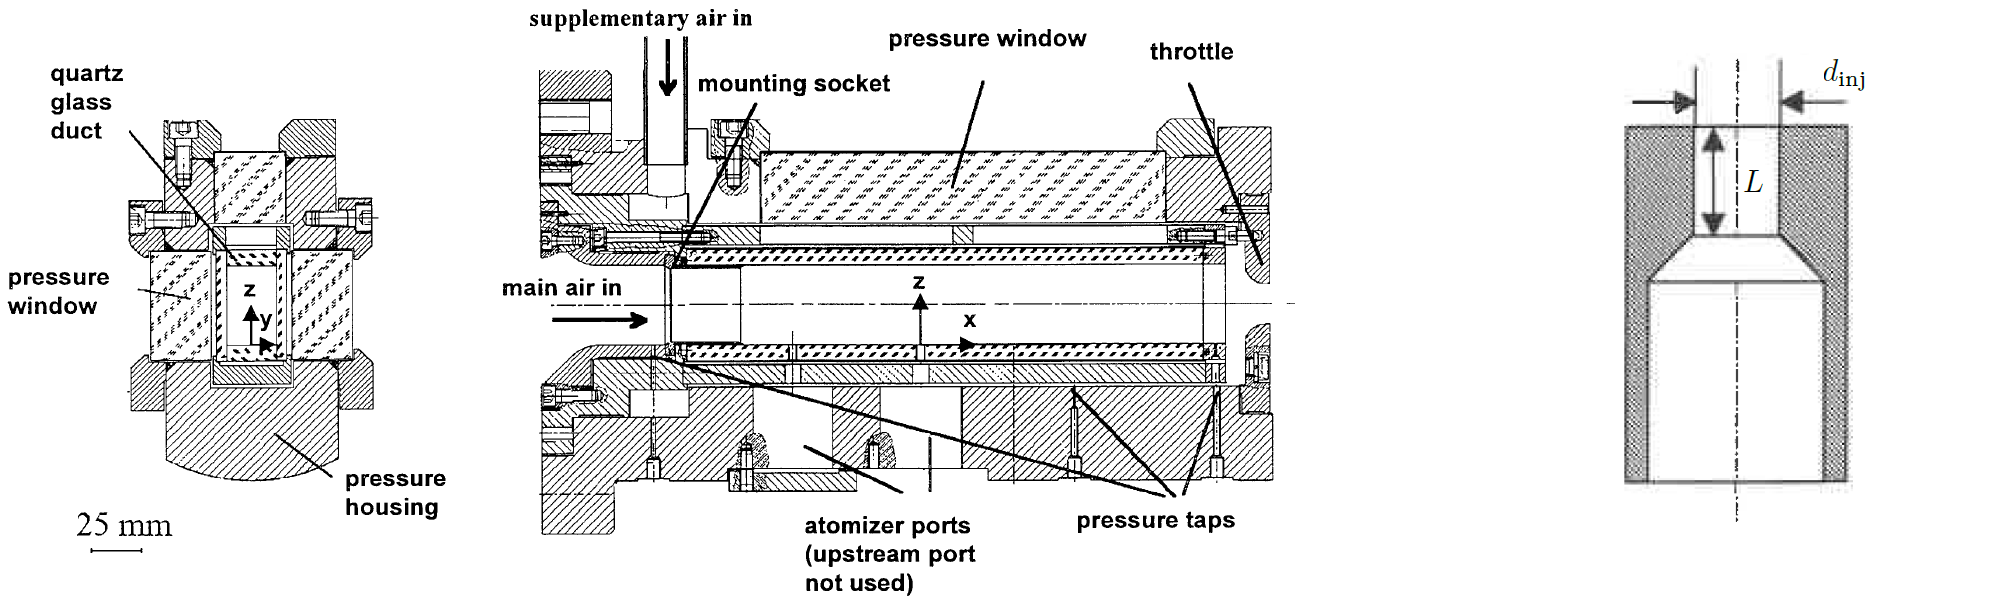
\includegraphics[scale=0.35]{./part2_developments/figures_ch5_resolved_JICF/experiment_JICF_DLR}
	\caption[JICF experimental setup]{JICF experimental setup. \textsl{Left}: Test rig. \textsl{Right}: liquid nozzle geometry employed in the experimental study. Source: \citeColor[becker_breakup_2002]}
	\label{fig:experiment_JICF_DLR}
\end{figure}




\section{Computational setup}
	\label{sec:computational_setup}

%\subsection*{Numerical domain and baseline mesh}

Figure \ref{fig:numerical_setup_maquette_JICF_DLR} shows the computational domain developed to replicate the simulations of the test bench from \citeColor[becker_breakup_2002]. The plenum is modeled as a box with dimensions 25x40x270 mm$^3$. The hydraulic diameter of the duct cross section, which is used to calculate the gas Reynolds number, is $D_h = 30.8$ mm. A magnified view of the nozzle is also shown, with diameter $0.45$ mm and straight section length of 0.7 mm prior to injection to keep $L/D = 1.56$ as in the experiments. The boundary conditions are also indicated. The plenum walls use a wall law of logarithmic type except closer to the domain pressure outlet, which have been set to slip walls to avoid backflow. The nozzle walls are rigid walls. For the liquid inlet, a Poiseuille profile has been specified, while in the gaseous inlet a mean velocity profile has been set in order to recover the boundary layer thickness of between 4 and 5 mm upstream the injection nozzle as described in the experiments (see Appendix \ref{app:JICF_BL_setup} for details). Due to the high Reynolds number at the gaseous inlet ($Re \sim O \left( 10^6 \right)$, see Table \ref{tab:jicf_operating_conditions}), synthetic turbulence is added in the liquid inlet.

\begin{figure}[ht]
     \centering
     \includeinkscape[scale=0.35]{./part2_developments/figures_ch5_resolved_JICF/DLR_becker_numerical_config}
      \caption{Numerical domain and boundary conditions of the experimental test bench of \citeColor[becker_breakup_2002]. \textsl{Left}: complete domain. \textsl{Right}: detailed view of the injection nozzle. All dimensions are in mm.}
      \label{fig:numerical_setup_maquette_JICF_DLR}
\end{figure}


Figure \ref{fig:jicf_dlr_mesh} shows the baseline mesh, where the symmetry plane $y = 0$ is displayed. It is composed of 66 million tetrahedral cells. The baseline cell size in the channel upstream liquid injection is 0.5 mm, which was chosen after performing a mesh independence study on the gaseous field (results in Appendix \ref{app:gas_initial_cond_JICF}). The cells located in the downstream region have an average size of 3 mm, and the element size within the discharge section of the liquid nozzle is refined to $20~\mu$m. This mesh is used at the beginning of all the simulations performed, which afterwards changes dynamically throughout the simulation as more liquid is introduced in the domain due to the Adaptive Mesh Refinement (AMR) routine. Simulations are performed with the ACLS methodology describe in $\S$\ref{subsec:ch2_ACLS}. Liquid is allowed to penetrate up to a certain $x$ location downstream the injector: at this location, a sponge layer is added to remove liquid artificially for restricting the region inside the plenum containing liquid, thus limiting the cost of the resolved simulations. The location of the sponge layers is detailed in the next section, since it depends on each performed simulation.

\begin{figure}[h!]
	\centering	\includeinkscape[inkscapelatex=false,scale=0.65]{./part2_developments/figures_ch5_resolved_JICF/jicf_mesh/jicf_mesh}
	\caption[Baseline JICF mesh, showing magnified views of the near-field and nozzle regions.]{Baseline JICF mesh, showing magnified views of the near-field and nozzle regions. The red rectangle is the region where meshes are shown in the mesh convergence study of Appendix \ref{app:gas_initial_cond_JICF}}
	\label{fig:jicf_dlr_mesh}
\end{figure}





\section{Operating conditions}
\label{sec:JICF_SPS_OPs_detailed}

Two operating conditions tested experimentally in \citeColor[becker_breakup_2002] have been simulated. Both of them have the same momentum ration $q = 6$ but differ in the Weber number: $We_g = 830$ (low Weber) and $We_g = 1470$ (high Weber), calculated with Eq. (\ref{eq:ch1_intro_Re_and_We_general_definitions}). According to the values of $q$ and $We_g$, the former condition corresponds to surface breakup dominating regime while the latter is located at the dividing line between column and surface breakup. Figure \ref{fig:location_JICF_ops_in_breakup_map} shows the location of both operating points in the breakup map of \citeColor[wu_breakup_1997]. The physical magnitudes and dimensionless numbers of both operating points are shown in Table \ref{tab:jicf_operating_conditions}. Apart from the values $q$ and $We_g$, the dimensionless numbers in  Eq. (\ref{eq:dimensionless_numbers_jicf}) are also calculated: the liquid and gaseous Reynolds numbers $Re_l$ and $Re_g$ respectively, Ohnesorge number $Oh$, aerodynamic Weber $We_\mathrm{aero}$, relative Weber $We_\mathrm{rel}$ and density ratio $r$. These numbers have been added since they are defined in several experimental studies \citemColor[wu_breakup_1997,becker_breakup_2002,ragucci_trajectory_2007] to characterize the operating points tested. 

Computations are performed with the ACLS methodology combined with the AMR routine described in $\S$\ref{subsec:ch2_ACLS}. For each operating condition, two interface cell sizes have been simulated: $\Delta x_\mathrm{min} = 20 ~\mu$m (coarse case) and $\Delta x_\mathrm{min} = 10 ~\mu$m (fine case). The levelset band around the interface, which denotes the region where the cell size is $\Delta x_\mathrm{min}$, has been set to 12 cells ($N_p = 12$ from Figure \ref{fig:AMR_strategy}). The nomenclature for each simulation, which is used hereafter in this document, is introduced in Table \ref{tab:jicf_resolved_simulations_performed}: cases indicate the operating point by its gaseous velocity (UG), the level-set resolution (DX), and an additional simulation with no synthetic turbulence (NT) injected has been performed.  The coarse cases locate the sponge layer to remove liquid at a downstream distance of $x = 16$ mm, while the fine ones place it at $x = 11$ mm. In such ways, droplets can be sampled up to planes $x = 15$ and $10$ mm respectively. The number of steps for the reinitialization equation (\ref{eq:acls_reinit_2017}) is set to $N_\mathrm{reinit} = 6$. This parameter has shown to affect mass conservation in the JICF simulations; its effect and the choice of this value are discussed in Appendix \ref{app:IBs_mass_conservation_ACLS}.


\begin{equation}
\label{eq:dimensionless_numbers_jicf}
\begin{aligned}
Re_l &= \frac{\rho_l u_l d_\mathrm{inj}}{\mu_l}          &  Re_g &= \frac{\rho_g u_g D_h}{\mu_g}              &  Oh &=  \frac{\mu_l}{\sqrt{\rho_l \sigma d_\mathrm{inj}}}\\
We_\mathrm{aero} &= \frac{\rho_g u_l^2 d_\mathrm{inj}}{\sigma}    &  We_\mathrm{rel} &= \frac{\rho_g \left( u_g - u_l \right)^2 d_\mathrm{inj}}{\sigma}          & r &= \frac{\rho_l}{\rho_g} 
\end{aligned}
\end{equation}

\begin{table}[!h]
\centering
\caption{Nomenclature for resolved atomization simulations}
\begin{tabular}{cccc}
\thickhline
\multirow{2}{*}{ $\Delta x_\mathrm{min}$ [$\mu$m] } & Turbulence & \multicolumn{2}{c}{\textbf{Operating condition}} \\ 
\cline{3-4}
 & injection ? & Low $We_g$ &  High $We_g$ \\ 
\thickhline
\textbf{10} & Yes & UG75\_DX10 & UG100\_DX10 \\
\textbf{20} & Yes & UG75\_DX20 & UG100\_DX20 \\
\textbf{20} & No & - & UG100\_DX20\_NT \\
\thickhline
\end{tabular}
\label{tab:jicf_resolved_simulations_performed}
\end{table}

\clearpage


\begin{table}[!h]
\centering
\caption{JICF operating points studied}
\vspace*{-0.1in}
\begin{tabular}{lcccc}
\thickhline
\textbf{Parameter} & \textbf{Symbol} & \textbf{Units} &  \textbf{Low Weber} &  \textbf{High Weber} \\ %\textbf{WE\_880} &  \textbf{WE\_1470} \\
\thickhline
Nozzle diameter & $d_\mathrm{inj}$ & mm & 0.45 & 0.45 \\
%\hline
Gas bulk velocity & $u_g$ & m s$^{-1}$ & 75 & 100 \\
%\hline
Gas flow rate & $Q_g$ & m$^3$ s$^{-1}$ & 0.075  & 0.1 \\
%\hline
Liquid bulk velocity & $u_l$ & m s$^{-1}$ & 17.5  & 23.33 \\
%\hline
Liquid flow rate & $Q_l$ & mm$^3$ s$^{-1}$ & 2783  & 3710 \\
%\hline
Ambient pressure & $p_\mathrm{amb}$ & bar &  6 & 6 \\
%\hline
Gas temperature & $T_g$ & K & 290 & 290 \\
%\hline
Liquid temperature & $T_l$ & K & 290 & 290 \\
%\hline
Gas density & $\rho_g$ & kg m$^{-3}$ &  7.21 & 7.21 \\
%\hline
Liquid density & $\rho_l$ & kg m$^{-3}$ &  795 & 795  \\
%\hline
Gas viscosity & $\mu_g$ & kg m$^{-1}$ s$^{-1}$ & $1.8162 \cdot 10^{-5}$ &  $1.8162 \cdot 10^{-5}$  \\
%\hline
Liquid viscosity & $\mu_l$ & kg m$^{-1}$ s$^{-1}$ & $1.5 \cdot 10^{-3}$ & $1.5 \cdot 10^{-3}$  \\
%\hline
Surface tension & $\sigma$ & kg s$^{-2}$ &  0.022 & 0.022  \\
\thickhline
Momentum ratio & $q$ & - & 6 & 6 \\
%\hline
Gas Reynolds number & $Re_g$ & - & $0.92 \cdot 10^6$ & $1.22 \cdot 10^6$ \\
%\hline
Liquid Reynolds number & $Re_l$ & - & 4170 & 5560 \\
%\hline
Gas Weber number & $We_g$ & - & 830 & 1470 \\
%\hline
Liquid Weber number & $We_l$ & - & 5000 & 8850 \\
%\hline
Relative Weber number & $We_\mathrm{rel}$ & - & 490 & 870 \\
%\hline
Aerodynamic Weber number & $We_\mathrm{aero}$ & - & 45 & 80 \\
%\hline
Ohnesorge number & $Oh $ & - & 0.017 & 0.017 \\
%\hline
Density ratio & $r$ & - & 110 & 110 \\
%\hline
%Viscosity ratio & $\mu_l/\mu_g$ & [-] &  \multicolumn{2}{|c|}{1} \\
\thickhline
\end{tabular}
\label{tab:jicf_operating_conditions}
\end{table}





\begin{figure}[ht]
     \centering
     \includeinkscape[inkscapelatex=false,scale=0.5]{./part2_developments/figures_ch5_resolved_JICF/jicf_breakup_regime_our_operating_points_LONG}
     \caption{Location of simulated operating conditions in the breakup map by \citeColor[wu_breakup_1997]}
	% See: https://stackoverflow.com/questions/35210337/can-i-plot-several-histograms-in-3d/35225919
      \label{fig:location_JICF_ops_in_breakup_map}
\end{figure}




\clearpage

\section{Gaseous initial conditions}
\label{sec:ch5_initial_conditions}

Prior to liquid injection, a gaseous field must be initialised in the computations. The objective is to obtain an established velocity profile that reproduces correctly the mean profile with a boundary layer thickness $\delta$ as observed in the experiments, which is reported to be between $4$ and $5$ mm \citepColor[becker_breakup_2002]. For this purpose, a mean profile is injected at the gaseous inlet shown in Figure \ref{fig:numerical_setup_maquette_JICF_DLR} formed by the combination of a boundary layer and a flat outer profile. The details on this mean profile are given in Appendix \ref{app:JICF_BL_setup}. Furthermore, the gaseous flow is turbulent, as shown by the high gaseous Reynolds number ($>> 10^4$) in the operating points studied (see Table \ref{tab:jicf_operating_conditions}). Therefore, synthetic turbulence is also injected at the gaseous inlet, hence a random fluctuating velocity component is added to the mean profile. This turbulence requires then a cell size that allows its transport in the mesh. For this purpose, a mesh independence study was performed, from which a mesh resolution $\Delta x = 0.5$ mm from the gaseous inlet until the liquid injection nozzle is chosen. This element size allows for a proper turbulent transport (frequencies
and energy content) with a moderable cost. Details on the injection of synthetic turbulence and the mesh independence study are discussed in Appendix \ref{app:gas_initial_cond_JICF}. 

Figure \ref{fig:ics_mean_profiles_op2} shows the profiles for gaseous mean axial velocity $\overline{u}$ and Turbulent Kinetic Energy (TKE), calculated as $TKE = \left( \overline{u'^2} + \overline{v'^2} + \overline{w'^2} \right) / 2$, for both operating points. As shown, a boundary layer thickness of around 5 mm is captured, reflected in both the $\overline{u}$ and $TKE$ profiles. This agrees with the values reported by \citeColor[becker_breakup_2002]. Part of the liquid jet is immersed within the boundary layer, as illustrated in Figure \ref{fig:Umean_profile_with_jet} where the velocity profile is plotted alongside an instantaneous view of a liquid jet from a resolved simulation. Since the TKE values are large within the boundary layer as shown in Figure \ref{fig:ics_mean_profiles_op2}b, it is probable that turbulence from the boundary layer plays a role in the jet primary breakup.

\begin{figure}[ht]
\centering
\begin{subfigure}[b]{0.45\textwidth}
	\centering
   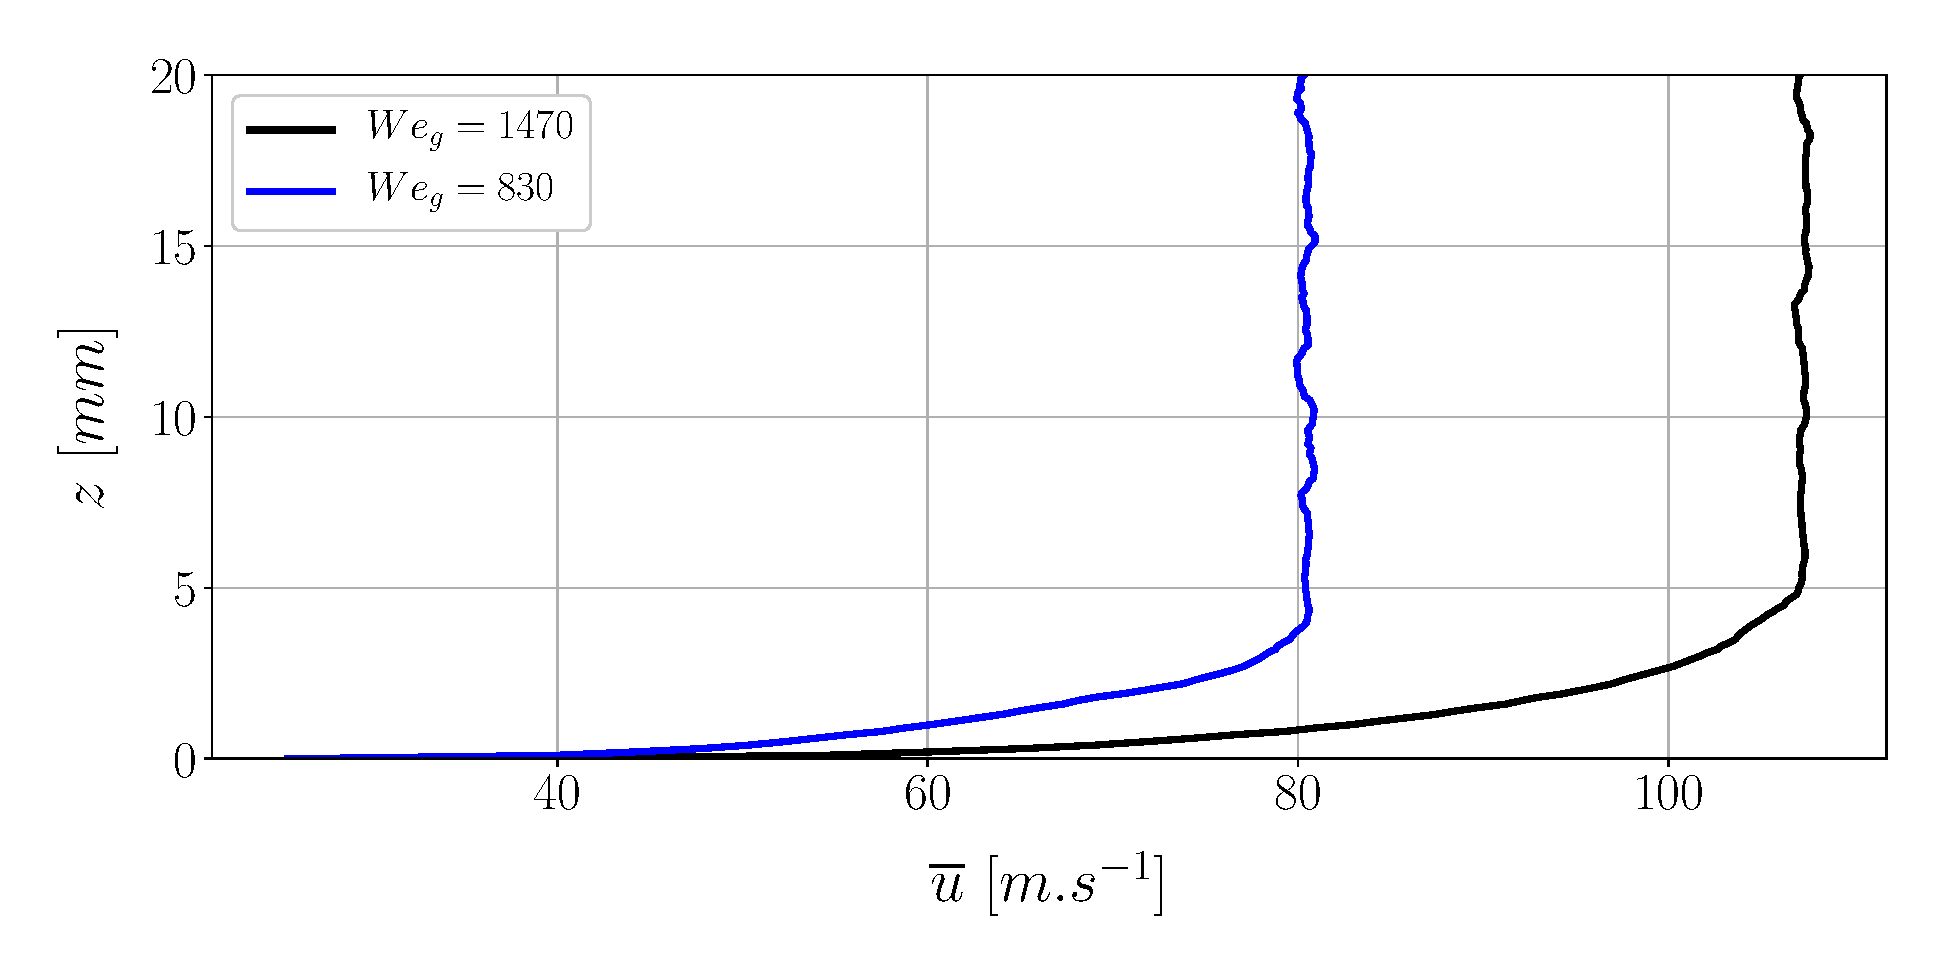
\includegraphics[scale=0.25]{./part2_developments/figures_ch5_resolved_JICF/results_ics_mesh_convergence_mean_profiles/U_MEAN_profiles_op2.pdf}
   \vspace*{-0.20in}
   \caption{Mean axial velocity}
   %\label{} 
\end{subfigure}
\hfill
\begin{subfigure}[b]{0.45\textwidth}
	\centering
   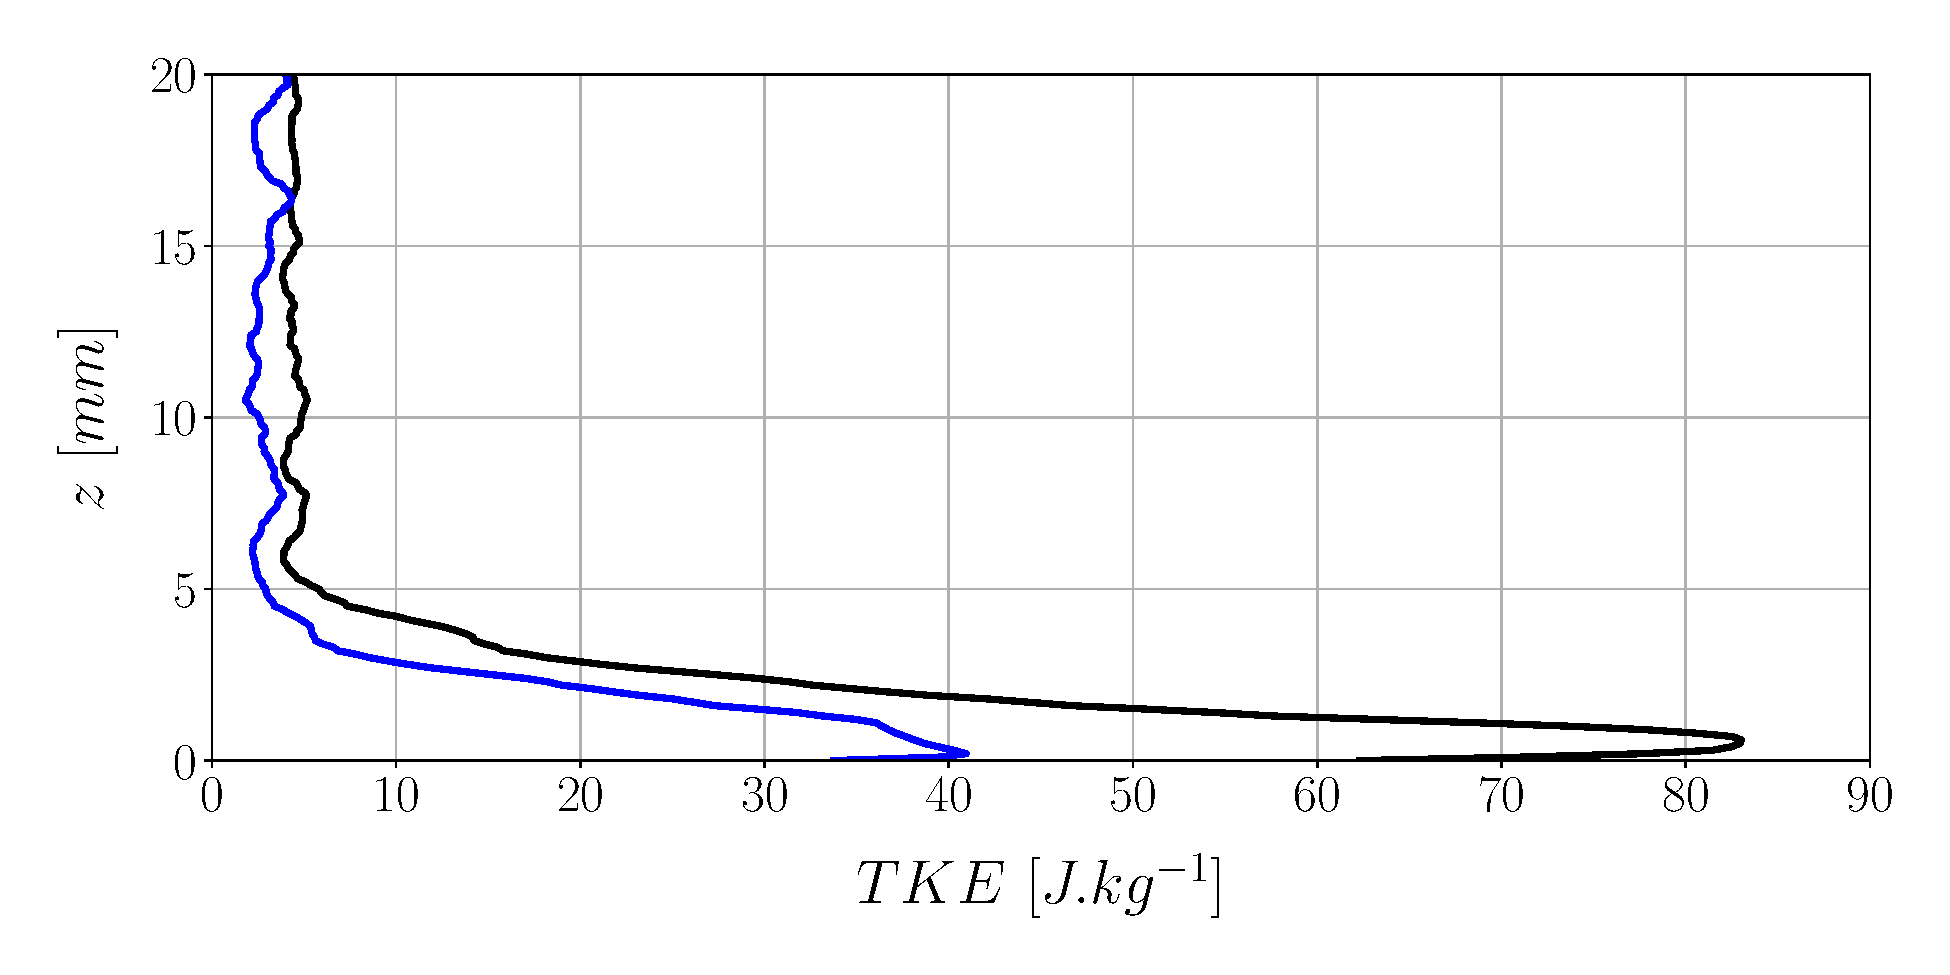
\includegraphics[scale=0.25]{./part2_developments/figures_ch5_resolved_JICF/results_ics_mesh_convergence_mean_profiles/TKE_profiles_op2.pdf}
   \vspace*{-0.20in}
   \caption{Turbulent Kinetic Energy}
   %\label{}
\end{subfigure}
\caption{Profiles of $\overline{u}$ and $TKE$ along the line right upstream the injector for both operating points for mesh resolution $\Delta x_\mathrm{ups} = 0.5$ mm.}
\label{fig:ics_mean_profiles_op2}
\end{figure}




\begin{figure}[ht]
\centering
\includegraphics[scale=0.2]{./part2_developments/figures_ch5_resolved_JICF/Umean_profile_with_jet_in_BL}
\caption[Instaneous JICF view with mean axial velocity field in symmetry plane $y = 0$]{Instaneous JICF view with mean axial velocity field in symmetry plane $y = 0$. The vectors represent the velocity profile just upstream the injector, showing the boundary layer thickness $\delta = 5$ mm. The velocity profile has been displaced upstream in the picture for a better visualization.}
% OJO: ficheros generados para el perfil de velocidades estan en Ongoing\ICS_study\u_mean_profiles\cases_probes\mesh_refined_DX0p5_ics_no_actuator_flat_BL_with_turbulence_L3p00_up2p7
\label{fig:Umean_profile_with_jet}
\end{figure}



\clearpage

\section{Analysis of JICF simulations}
\label{sec:ch5_JICF_simus_analysis}

This section reports and analyzes several physical features from the JICF configurations, including a validation with an experimental correlation for the jet's vertical trajectory. The data here presented are of interest to verify the capability of resolved simulations for accurately capturing the physics and dynamics of atomization.

\subsection{Jet evolution}
\label{subsec:ch5_jet_evolution}




%\subsection{Flow establishment}
%\label{subsec:ch5_JICF_flow_establishment}

Figures \ref{fig:JICF_establishment_UG100_lateral} to \ref{fig:JICF_establishment_UG75_top} shows the evolution of the jet for all the simulations in three different view: lateral, front and top. The left column shows the thicker resolution, while the right column shows the finer one. The interface is represented by the iso-value $\psi = 0.5$. The snapshots correspond to the same time instants in all cases, which are expressed in dimensionless units with respect to the liquid inertia timescale $\tau_\mathrm{in}$:

\begin{equation}
\label{eq:t_dimensionless_with_tau_in}
t^* = \frac{t}{\tau_\mathrm{in}}
\end{equation}

with $\tau_\mathrm{in} = d_\mathrm{inj}/u_l$. This timescale is widely used in literature to express the establishment of liquid jets in crossflow \citepColor[herrmann_impact_2011]. Applying this formula to each operating condition results in values of $\tau_\mathrm{in} = $ 25.72 and 19.29 $\mu$s for the low and high Weber cases, respectively. Since the values for $\tau_\mathrm{in}$ are different for both operating points, the absolute times from injection are not the same for each condition. However, due to the different injection velocities in each case, the introduction of the timescale $t^*$ allows for a proper comparison among jets from different operating conditions.

%for the same time instant $t^*$, the low-We point represents a more advanced physical time than the high-We case. This allows to compare the jets at equivalent times among operating conditions, since they differ in the characteris: since the low-We operating point involves lower gas and liquid velocities, the jet has advanced in a lesser extent than the high-We case for the same absolute time instant. Therefore, expressing a dimensionless time with respect to a reference time that takes into account the difference in velocity between both cases (in this case, the one of the liquid phase) allows for a more representative comparison of both jets.

The lateral view of the jets show that the jet leaves the nozzle in the vertical direction and then bends towards the crossflow. For both operating points and both resolutions, droplets are stripped off the sides of the liquid column shortly after injection (surface breakup) and are convected downstream the crossflow direction. The finer resolution shows more droplets generated by surface breakup than the coarse one. Further downstream, the jet is deformed due to the crossflow impact and momentum exchange, leading to the breakup of the liquid column into big ligaments (column breakup). It is also noticeable in the instantaneous snapshots of Figures \ref{fig:JICF_establishment_UG100_lateral} and \ref{fig:JICF_establishment_UG75_lateral} that the jet vertical trajectory differs with resolution: fine simulations penetrate further vertically than the coarse ones. This is due to the resolution of instabilities, since the ligaments generated in the fine simulation contain more inertia and therefore will travel further than the ones generated in the coarse mesh. The resulting trajectories are quantifed and compared later in $\S$\ref{subsec:ch5_jet_trajectories_results}, confirming these observations from the qualitative figures. It is also worth to mention that resulting trajectories are not dependent on the operating point simulations (for identical mesh resolutions), which is in line with the experimental observations (see Table \ref{tab:correlations_experimental_JICF}) since the momentum flux ratio $q = 6$ is identical for both simulations and trajectories are believed to be solely dependent on this factor.

Front views of the jets are shown in Figures \ref{fig:JICF_establishment_UG100_front}, \ref{fig:JICF_establishment_UG75_front} for each operating point, while the top views are seen in \ref{fig:JICF_establishment_UG100_top}, \ref{fig:JICF_establishment_UG75_top}. The front views show clearly the windward instabilities in the fine case, which extend along all the width of the liquid column. These ones are generated right at the vicinity of the injector, observed through the corrugations at these region which are developed and amplified further downstrea. The top views show the lateral opening of the jet along the crossflow direction: the fine jets show a wider dense core than the coarse ones (a quantitative analysis on the dense core topology is later provided in$\S$\ref{subsec:ch5_DC_topology_characterization}), and the subsequent spray formed after atomization presents also a larger span in the lateral direction for the former than for the latter.


\clearpage

\begin{figure}[ht]
\centering
\includeinkscape[inkscapelatex=false,scale=0.8]{./part2_developments/figures_ch5_resolved_JICF/JICF_establishment_UG100_lateral}
\caption[Lateral view of high We jet at several time instants. ]{Lateral view of high We jet at several time instants. \textsl{Left}: UG100\_DX20. \textsl{Right}: UG100\_DX10.}
\label{fig:JICF_establishment_UG100_lateral}
\end{figure}

\clearpage

\begin{figure}[ht]
\centering
\includeinkscape[inkscapelatex=false,scale=0.8]{./part2_developments/figures_ch5_resolved_JICF/JICF_establishment_UG100_front}
\caption[Front view of high We jet at several time instants. ]{Front view of high We jet at several time instants. \textsl{Left}: UG100\_DX20. \textsl{Right}: UG100\_DX10.}
\label{fig:JICF_establishment_UG100_front}
\end{figure}


\clearpage

\begin{figure}[ht]
\centering
\includeinkscape[inkscapelatex=false,scale=0.8]{./part2_developments/figures_ch5_resolved_JICF/JICF_establishment_UG100_top}
\caption[Top view of high We jet at several time instants. ]{Top view of high We jet at several time instants. \textsl{Left}: UG100\_DX20. \textsl{Right}: UG100\_DX10.}
\label{fig:JICF_establishment_UG100_top}
\end{figure}




\clearpage

\begin{figure}[ht]
\centering
\includeinkscape[inkscapelatex=false,scale=0.8]{./part2_developments/figures_ch5_resolved_JICF/JICF_establishment_UG75_lateral}
\caption[Lateral view of low We jet at several time instants. ]{Lateral view of low We jet at several time instants. \textsl{Left}: UG75\_DX20. \textsl{Right}: UG75\_DX10.}
\label{fig:JICF_establishment_UG75_lateral}
\end{figure}

\clearpage

\begin{figure}[ht]
\centering
\includeinkscape[inkscapelatex=false,scale=0.8]{./part2_developments/figures_ch5_resolved_JICF/JICF_establishment_UG75_front}
\caption[Front view of low We jet at several time instants. ]{Front view of low We jet at several time instants. \textsl{Left}: UG75\_DX20. \textsl{Right}: UG75\_DX10.}
\label{fig:JICF_establishment_UG75_front}
\end{figure}

\clearpage

\begin{figure}[ht]
\centering
\includeinkscape[inkscapelatex=false,scale=0.8]{./part2_developments/figures_ch5_resolved_JICF/JICF_establishment_UG75_top}
\caption[Top view of low We jet at several time instants. ]{Top view of low We jet at several time instants. \textsl{Left}: UG75\_DX20. \textsl{Right}: UG75\_DX10.}
\label{fig:JICF_establishment_UG75_top}
\end{figure}

\clearpage

\subsubsection*{Liquid establishment}

At the early instants of the injection process, the quantity of liquid in the domain increases with time. Then, the jet reaches the axial location where liquid is suppressed to avoid transporting droplets further downstream and hence reducing computational resources (sponge layer): from this time instant onwards, the liquid quantity in the domain remains at a constant value, and the jet is considered to be established. Since dynamic mesh adaptation is used to locate the smallest mesh elements in the liquid-gas interface (as explained in $\S$\ref{subsec:ch2_ACLS}), the mesh size increases with time as the interface surface within the domain is larger. An example of different meshes produced by each interface resolution is shown in Figure \ref{fig:JICF_w_mesh}. The physical time instant is the same for both simulations, corresponding to early injection. A cut of the mesh in the plane $y = 0$ is depicted, which shows how the regions where there is liquid contain much more elements than those which do not. The fine jet also shows liquid droplets further downstream that are not generated in the coarse one, hence there are refined spatial regions in the former that are not observed in the later.




\begin{figure}[ht]
\centering
	\centering
   %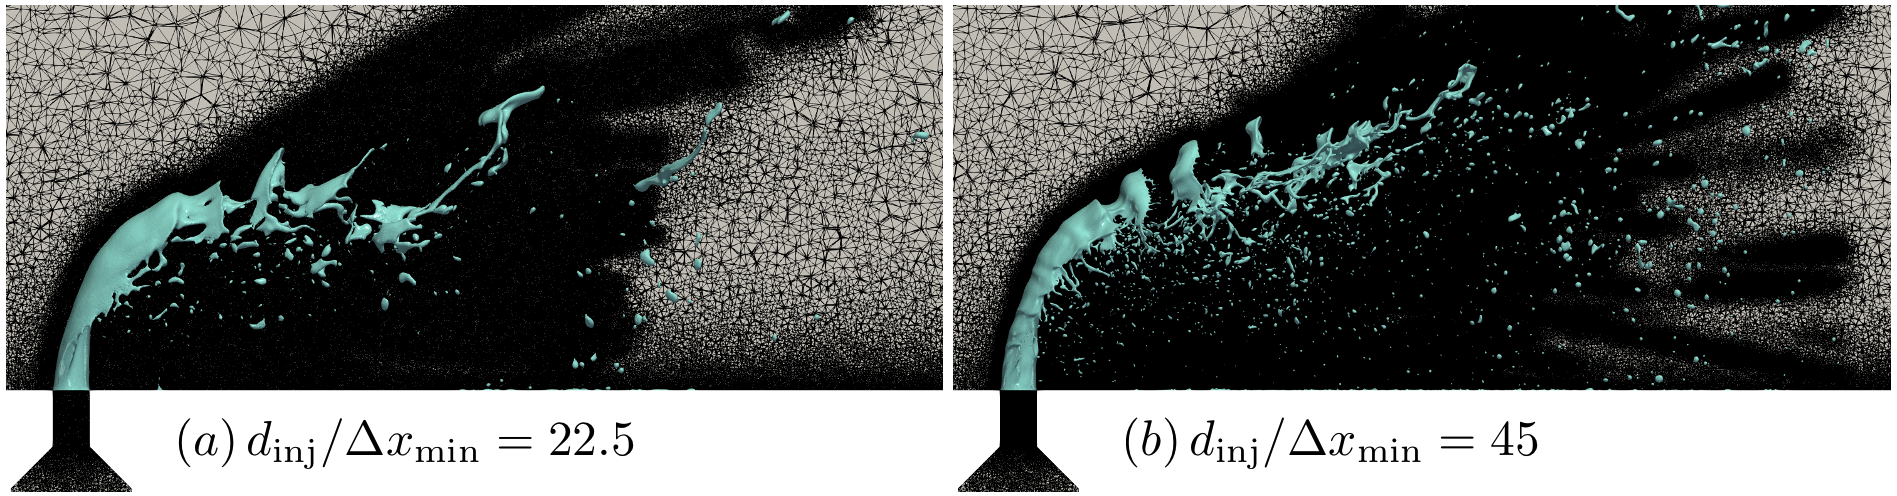
\includegraphics[scale=0.25]{./part2_developments/figures_ch5_resolved_JICF/JICF_nelem_evolution/JICF_w_mesh}
\includeinkscape[inkscapelatex=false,scale=0.75]{./part2_developments/figures_ch5_resolved_JICF/JICF_nelem_evolution/JICF_w_mesh}
   %\label{} 
\caption[Lateral view of meshes and interface contours near the injector at instant $t^{*}$ = 16 for the high Weber operating condition.]{Lateral view of meshes and interface contours near the injector at instant $t^{*}$ = 16 for the high Weber operating condition. \textsl{Left}: simulation UG100\_DX20. \textsl{Right}: simulation UG100\_DX10. Zoomed-in views of the rectangles are given in Figure \ref{fig:JICF_instabilities_lambda}.}
\label{fig:JICF_w_mesh}
\end{figure}

To illustrate a qualitative evolution with time of different quantities, the dimensionless time $t^{\prime} $ is used:

\begin{equation}
\label{eq:t_prime_with_tau_drx10}
t^{\prime} = \frac{t}{\tau_\mathrm{dr_{x=10}}}
\end{equation}

where $\tau_\mathrm{dr_{x=10}}$ is the arrival time of the first droplet to the sampling plane at $x = 10$ mm depicted in Figure \ref{fig:jicf_interior_boundaries_surface_measurements}. The plane $x = 10$ mm has been chosen because it is the last plane where liquid is sampled before being artificially removed in the fine simulations with $\Delta x_\mathrm{min} = 10 ~\mu$m, and is a sampling plane common to all simulations performed. Table \ref{tab:jicf_characteristic_droplet_sampling_times} shows the droplets arrival times to the different sampling planes in all simulations. 

\begin{table}[!h]
\centering
\caption{Droplet arrival times to sampling planes $\tau_\mathrm{dr_x}$ from JICF simulations [$\mu$s]}
\begin{tabular}{cccc}
\thickhline
\multirow{2}{*}{ \textbf{Case}} &  \multicolumn{3}{c}{$\tau_\mathrm{dr_x}$} \\
\cline{2-4}
 & $x = 5$ mm & $x = 10$ mm & $x = 15$ mm  \\
\thickhline 
UG75\_DX10  & 192.7 & 295.2 & -  \\
UG75\_DX20  & 234.7 & 355.8 & 456.7 \\
UG100\_DX10 & 143.7 & 218.7 & - \\
UG100\_DX20 & 176.8 & 258.4 & 362.8 \\
UG100\_DX20\_NT & 167.9 & 260.2 & - \\
\thickhline
\end{tabular}
\label{tab:jicf_characteristic_droplet_sampling_times}
\end{table}
In order to check the jet establishment in the domain, firstly the evolution of liquid volume with time is monitorded. This quantity can be obtained by integrating the level-set function $\psi$ in all the domain at each time instant:

\begin{equation}
\label{eq:liquid_volume_from_levelset_definition}
V_l \left ( t \right) = \int_{\Omega} \psi \left( \textbf{x}, t \right) d\textbf{x}
\end{equation}

The evolution of $V_l$ for each simulation is shown in 
Figure \ref{fig:JICF_liquid_volume_increase}. The volume increases linearly at the first instants in all cases, since the injected liquid flow rate is constant. As indicated in Table \ref{tab:jicf_operating_conditions}, flow rates are different for each operating point: nevertheless, the zoomed-in view shows that the slope of the $t^{\prime}$-$V_l$ is identical among resolutions, but differs among operating points. This is due to the timescales used to define $t^{\prime}$ from the physical time $t$: for identical operating condition, the first droplet to reach the sampling plane $x = 10$ mm arrives earlier in the fine case than in the coarse one. For identical resolutions, the droplets will reach the sampling plane earlier in the high Weber point than in the low one: as a consequence, the scaling balances out and the curves are overlapped in the linear region. Shortly after $t^{\prime} = 1$ (times when the first droplet reach plane $x = 10$ mm), the simulations for which liquid is suppressed after this axial location stabilize towards a constant liquid volume (with variations due to the amount droplets being suppresed, which changes at each time instant). Case UG100\_DX20\_NT reaches convergence in liquid volume quantity, while cases UG75\_DX10 and UG100\_DX10 (fine resolution simulations) are on the verge of this liquid stabilizing value, showing that they have reached a steady state. They have not run longer due to their high computational cost (details provided in $\S$\ref{subsec:ch5_computational_performances}). Simulations for which liquid is suppressed further downstream at $x = 15$ mm (UG75\_DX20, UG100\_DX20) achieve a stabilized liquid volume larger than the other cases, and reach this establishment at a later time.


\begin{figure}[ht]
\centering
	\centering
   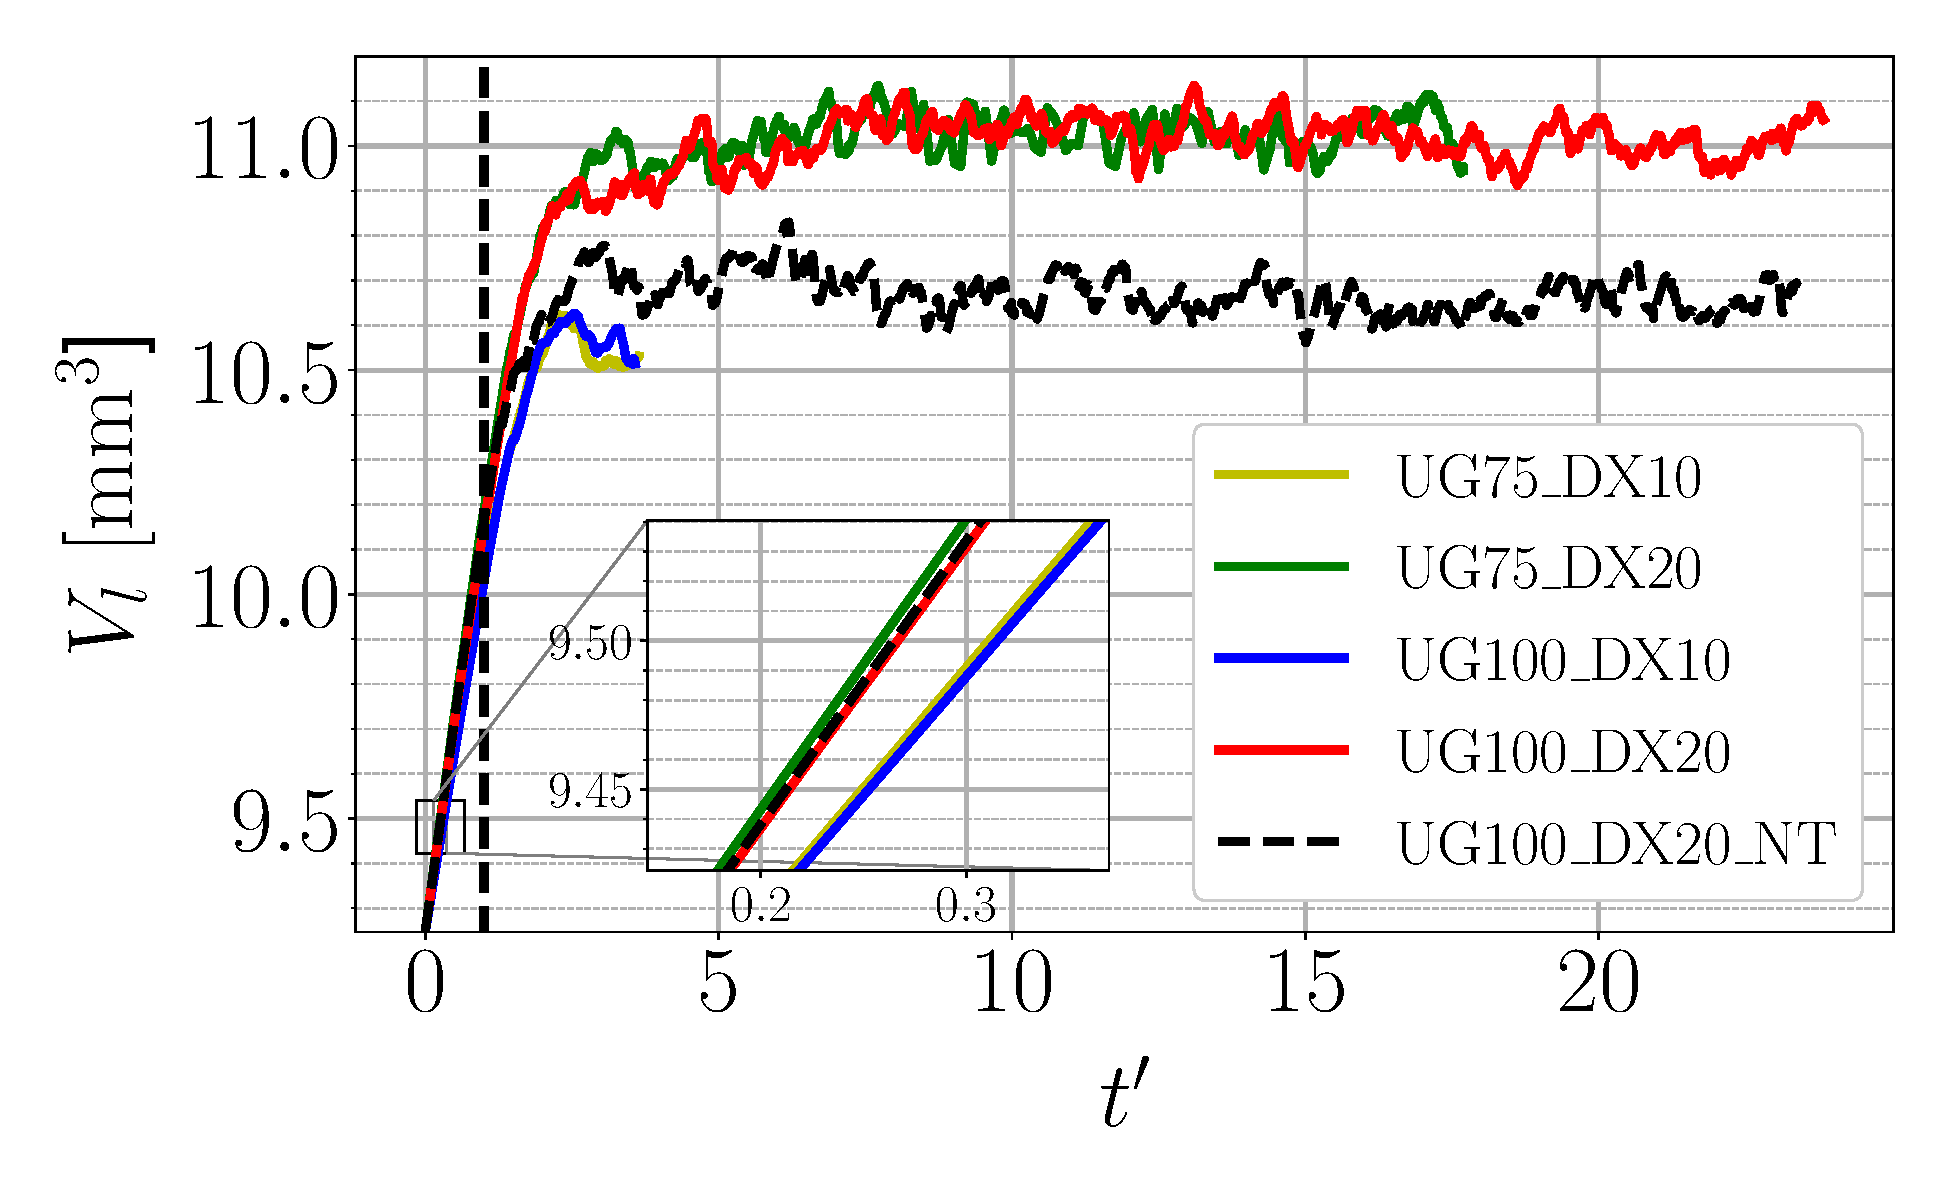
\includegraphics[scale=0.3]{./part2_developments/figures_ch5_resolved_JICF/JICF_liquid_volume_increase}
   \vspace*{-0.15in}
   \caption[Evolution of liquid volume with time in JICF simulations.]{Evolution of liquid volume with time in JICF simulations. The dashed, black vertical line corresponds to $t^\prime = 1$, time instant when the first droplet reaches the sampling plane $x = 10$ mm.}
\label{fig:JICF_liquid_volume_increase}
\end{figure}

The evolution of mesh size with time, given by the number of mesh elements ($N_\mathrm{elements}$), is shown in Figure \ref{fig:JICF_nelem_increase} for all simulations. For the fine simulations, the final number of elements is larger than in the coarse ones despite liquid being suppressed further upstream. The contrast is notorious, differing by one order of magnitude: for instance, in the high Weber simulations the simulation UG100\_DX20 contains 346$\cdot 10^6$ elements while case UG100\_DX10 ends at 1815$\cdot 10^6$ elements. By looking at Figure \ref{fig:JICF_nelem_increase}a, one can see that the number of elements increases slowly at the beginning and then rises exponentially (linearly in the semi-logarithmic plot) until there’s enough liquid in the domain and steady-state is reached. The first slow increase, which last for a short time, is associated to the increase of liquid volume due to jet injection prior to its fragmentation; the exponential increase is then associated to the creation of ligaments and droplets due to the atomization process, as the liquid-gas specific surface increases and therefore more elements are generated by the ARM process. Figure \ref{fig:JICF_nelem_increase_t_0_to_2} reveals the transition from the slow increase to the exponential rise in $N_\mathrm{elements}$ to occur at $t \sim 0.3$ for the fine simulations and at $t \sim 0.5$ for the coarse ones, which agrees with the earlier atomization observed in the fine cases (see for instance Figure \ref{fig:JICF_establishment_UG100_lateral}).



The dashed line in Figures \ref{fig:JICF_nelem_increase_all_t} and  \ref{fig:JICF_nelem_increase_t_0_to_2} corresponds  to $t^{\prime} = 1$, which is the instant at which the sampling plane $x = 10$ mm detects the first droplet in each simulation. Figure \ref{fig:JICF_nelem_increase_t_0_to_2} shows that this instant is located in the exponential region. Previously, there is no liquid being artificially removed in the simulations, so the curves increase monotonically (except for some minor decreases due to small droplets that reach the size of mesh resolution and disappear due to the unability of being further propagated in the simulations). After this point, the number of elements continues to increase exponentially up to $t^{\prime} \sim 1.5$ when the slope starts to decrease and, finally, the number of elements  stabilizes. Right after $t^{\prime} \sim 1.5$ there is a considerable amount of liquid droplets reaching the articifial sponge layer and being removed. Nevertheless, at this stage there are more droplets being generated in the near-nozzle region due to the disturbance effect of the liquid dense core to the air, which creates gaseous turbulence that helps to atomize ligaments ejected from the dense core. This explains the monotonic increase in the number of elements for $t^{\prime} > 1$ prior to its establishment around a constant value, which depends on each simulation. The only noticeable difference at $t^{\prime} = 1$ is for the simulation UG75$\_$DX10, which shows an abrupt reduction. Two reasons might explain this decrease. First, there is not only one droplet, but several ones reaching the last sampling plane, hence these droplets are all simultaneously removed from the simulation. Since the mean diameter of the droplets generated in a liquid JICF is larger when the air dynamic pressure is lower \citepColor[becker_breakup_2002], which is the case for the low Weber operating point, the droplets generated in this case are in general larger than for the high Weber case (this is later shown in $\S$\ref{subsec:ch5_sec_spray_characterization}), so all these droplets contain more elements than one single droplet from the case UG75\_DX10 and the removed amount liquid is larger. The second hypothesis is that, at this time instant, several liquid structures with size comparable to the mesh resolution limit disappear simultaneously when transported to the next timestep (a discussion on droplets disappearing due to this numerical phenomenon is given in Appendix \ref{app:IBs_mass_conservation_ACLS}
), causing an overall decrease in the number of elements. The combination of both could also occur, which combined would induce a larger decrease in the number of elements than if every single one acts separately.


\begin{figure}[ht]
\flushleft
\begin{subfigure}[b]{0.45\textwidth}
	\centering
   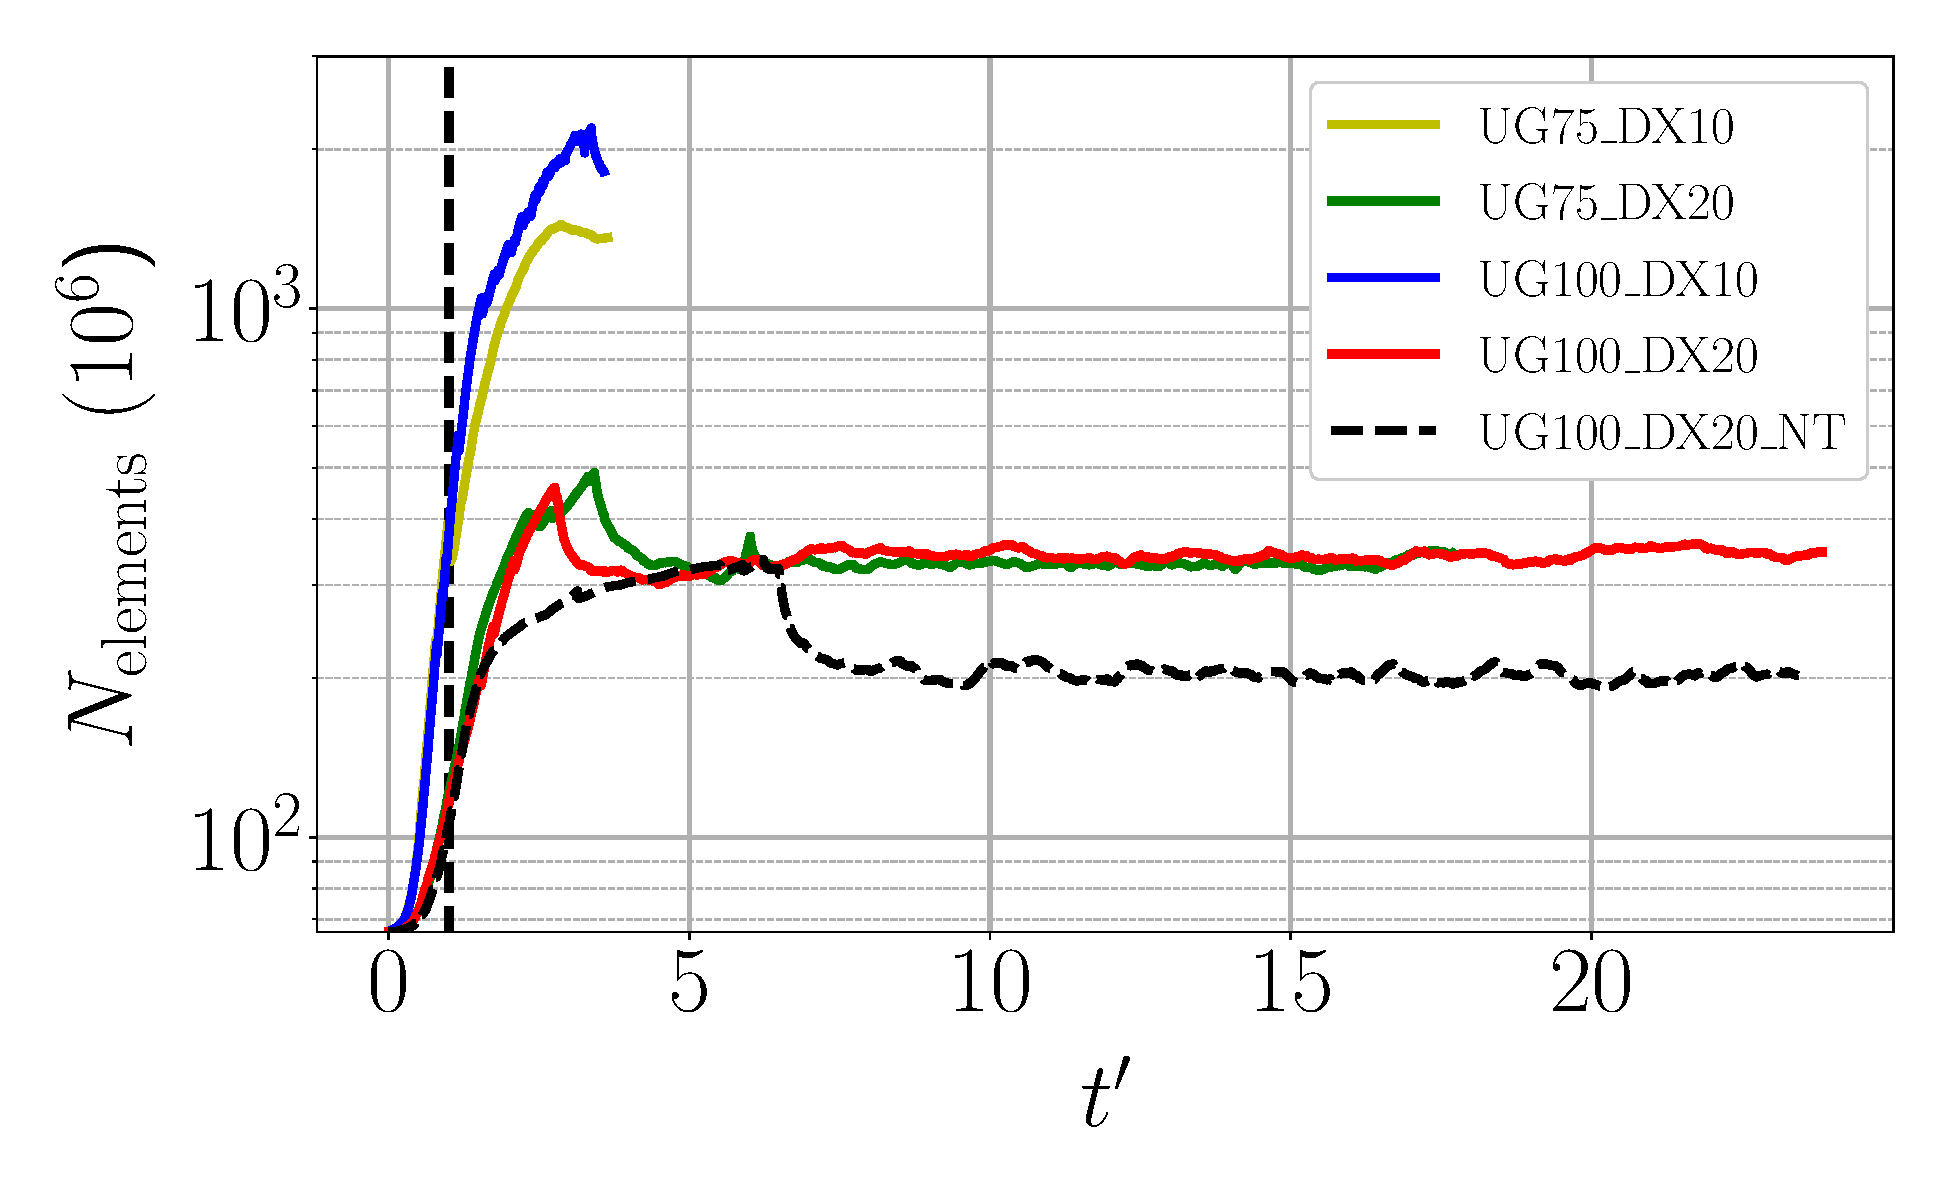
\includegraphics[scale=0.24]{./part2_developments/figures_ch5_resolved_JICF/JICF_nelem_evolution/JICF_nelem_increase}
   \vspace*{-0.25in}
   \caption{Evolution in simulations}
   \label{fig:JICF_nelem_increase_all_t} 
\end{subfigure}
\hfill
\begin{subfigure}[b]{0.45\textwidth}
	\centering
   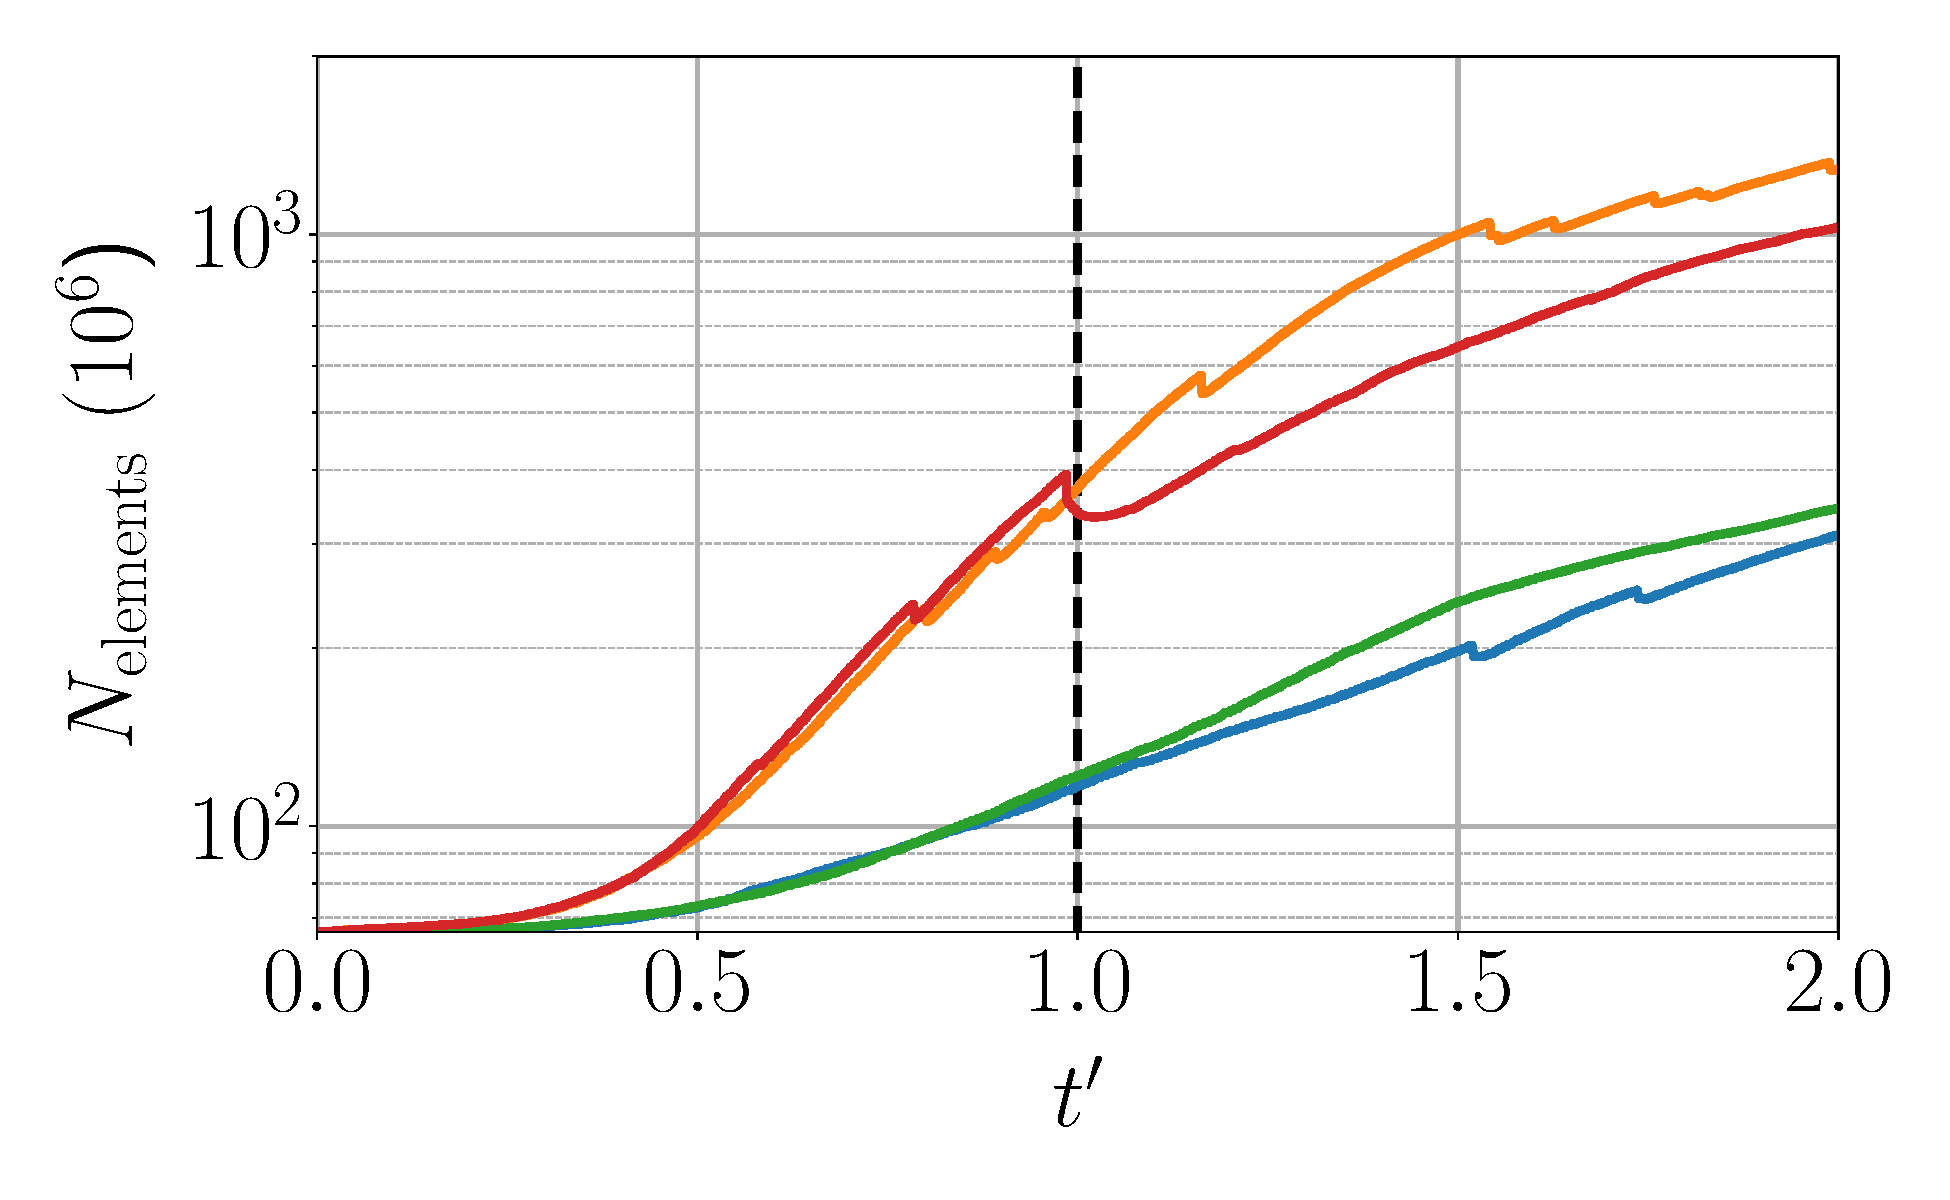
\includegraphics[scale=0.24]{./part2_developments/figures_ch5_resolved_JICF/JICF_nelem_evolution/JICF_nelem_increase_t_in_0_2}
   \vspace*{-0.25in}
   \caption{Zoomed-in view of Figure \ref{fig:JICF_nelem_increase_all_t} in range $t^{\prime} \in [0, 2]$}
   \label{fig:JICF_nelem_increase_t_0_to_2}
\end{subfigure}

%\vskip\baselineskip
%
%\begin{subfigure}[b]{0.45\textwidth}
%	\centering
%   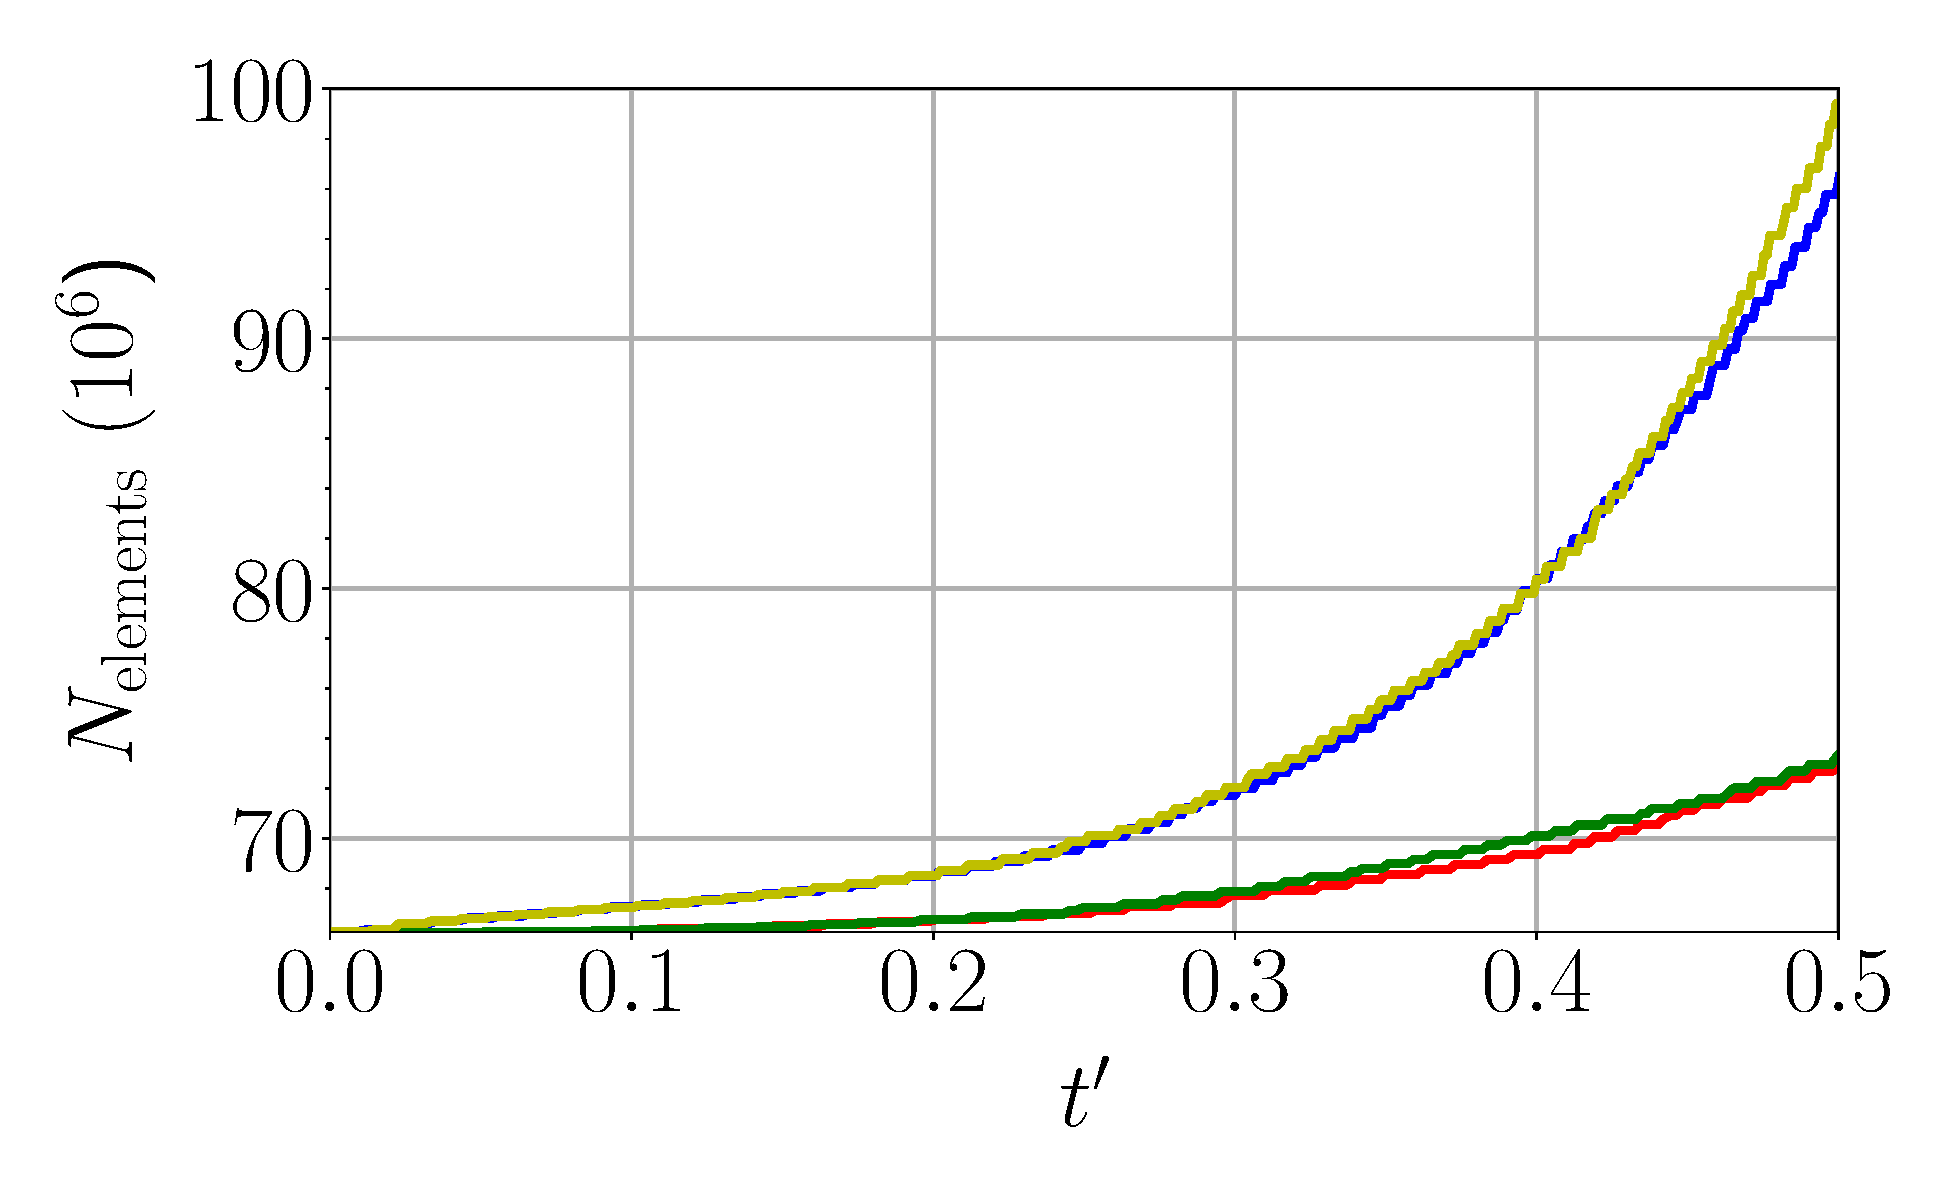
\includegraphics[scale=0.25]{./part2_developments/figures_ch5_resolved_JICF/JICF_nelem_evolution/JICF_nelem_increase_t_in_0_0p5}
%   \caption{Zoomed-in view in black rectangle of Figure \ref{fig:JICF_nelem_increase_t_0_to_2}}
%   \label{fig:JICF_nelem_increase_t_0_to_0p5} 
%\end{subfigure}
%\hfill
%\begin{subfigure}[b]{0.45\textwidth}
%	\centering
%   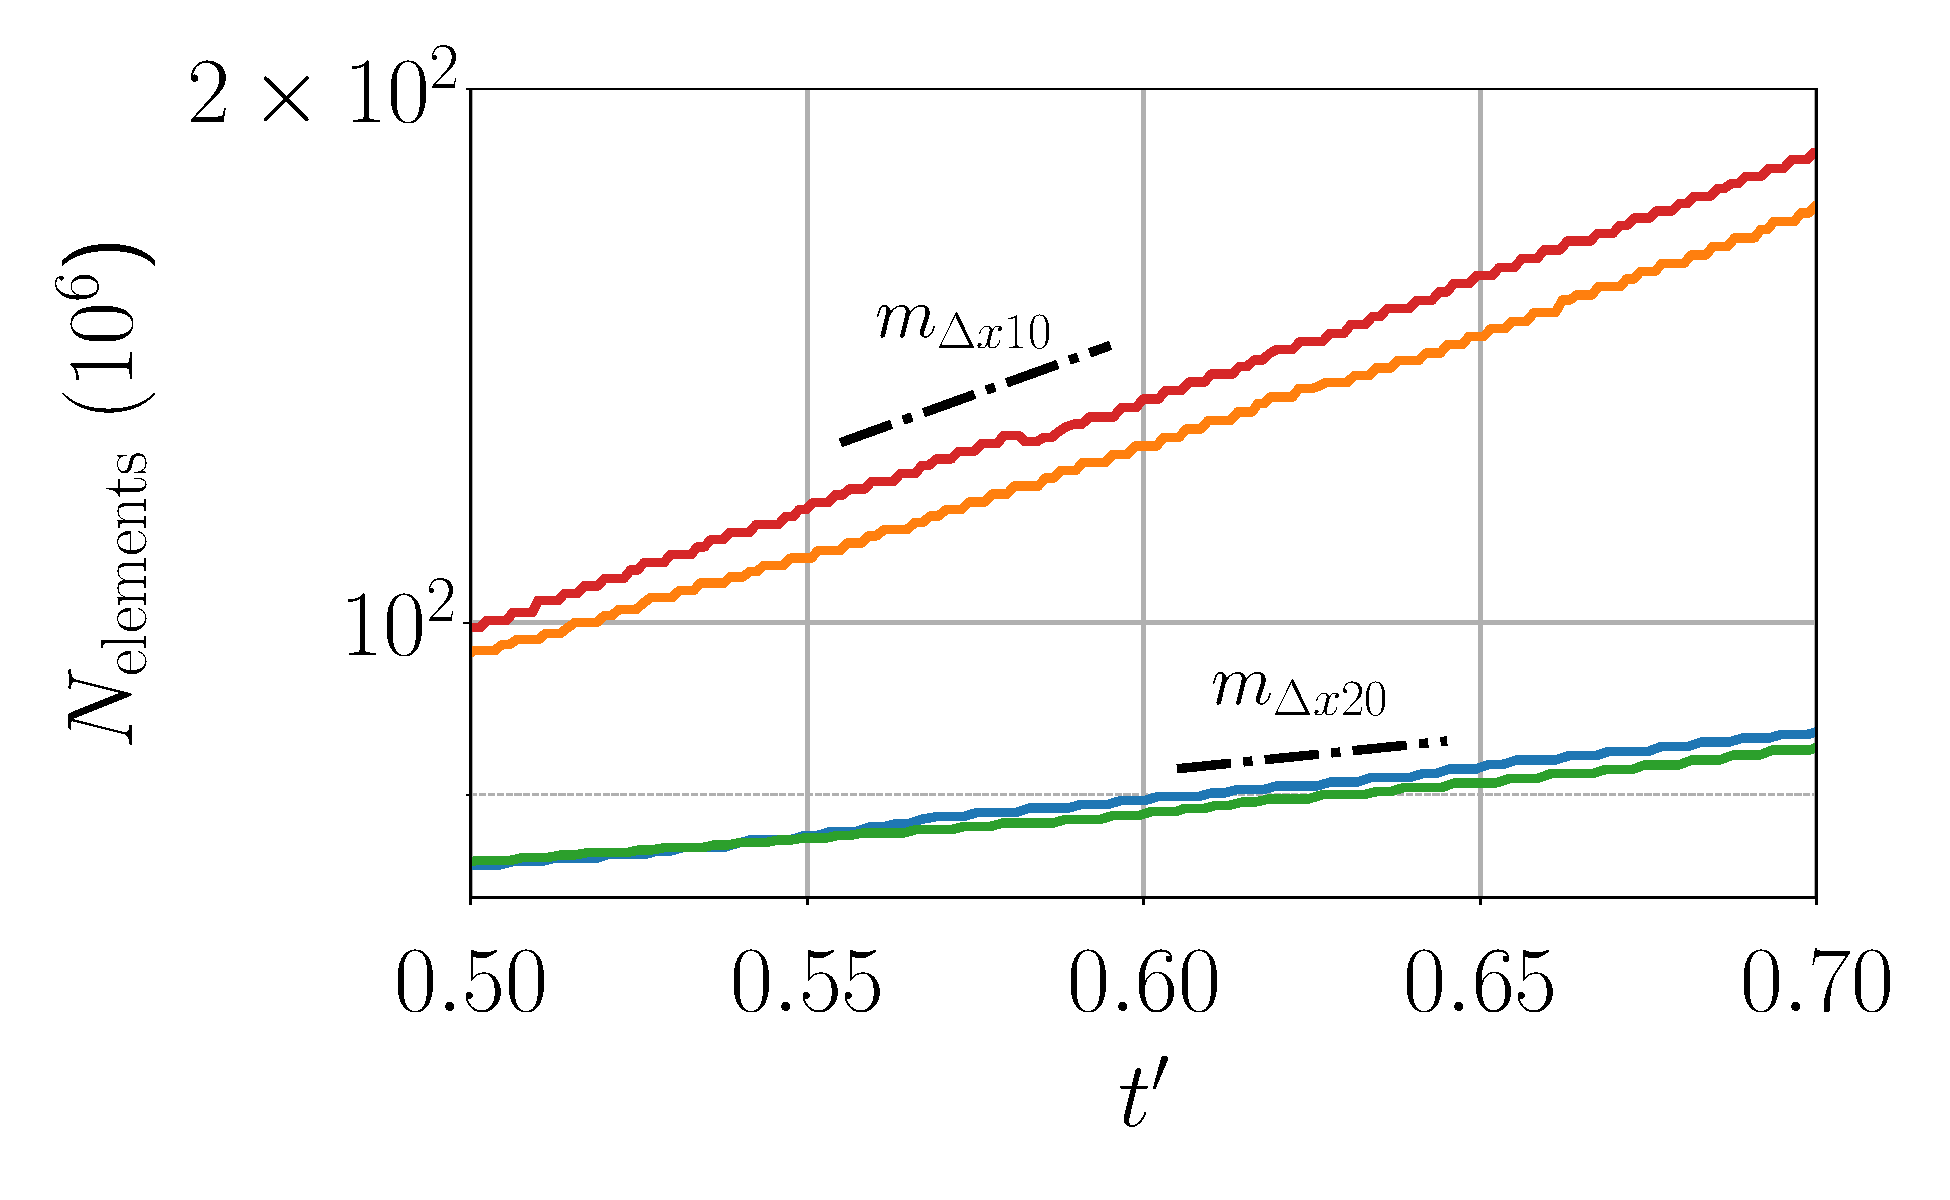
\includegraphics[scale=0.25]{./part2_developments/figures_ch5_resolved_JICF/JICF_nelem_evolution/JICF_nelem_increase_t_in_0p5_1}
%   \caption{Zoomed-in view in blue rectangle of Figure \ref{fig:JICF_nelem_increase_t_0_to_2}}
%   \label{fig:JICF_nelem_increase_t_0p5_to_0p7}
%\end{subfigure}
   \caption[Evolution of mesh size with time in JICF simulations]{Evolution of mesh size with time in JICF simulations. The dashed, black vertical line corresponds to $t^\prime = 1$, time instant when the first droplet reaches the sampling plane $x = 10$ mm.}
\label{fig:JICF_nelem_increase}
\end{figure}

\subsection{Breakup topology}
\label{subsubsec:ch5_breakup_topology}

In a liquid JICF, the most common primary atomization mechanisms are column and surface breakup (see $\S$\ref{sec:ch1_fuel_injection_technology} for a literature review on the topic). Both mechanisms are also identified in the resolved simulations performed. The \textbf{surface breakup} phenomenon is illustrated in Figure \ref{fig:jicf_surface_breakup_ug75_dx10}. Two regions are analyzed at the side of the jet: region A shows a zoomed-in view closer to the liquid injector, while region B details surface breakup taking place further downstream. Closer to the injector (region A), surface breakup is caused by lateral instabilities developed as a consequence of the strong shear force exerted by the incoming air, which forms corrugations at the surface \citepColor[behzad_surface_2016]. Droplets generated in this region do not undergo further breakup since they are very small (see the green and red ellipses, which follow the droplets generated from the corrugations) and, often, of the order of mesh resolution: most of these droplets will disappear when the levelset function is transported in the simulations. This issue is discussed later in $\S$\ref{subsec:ch5_direct_measurement_fluxes_IB}. Further downstream (region B), the jet is more deformed and surface breakup generates ligaments that separate from the main core and then undergo classical atomization: enclosed in red, the formation process of a ligament and its breakup into three smaller, different ligaments is depicted. As shown, this process forms liquid structures which are not spherical and can undergo further atomization, even though this one still occurs close to the jet dense core and the formed structures will be in equilibrium with the ambient gas shortly afterwards.

\clearpage

\begin{figure}[ht]
\centering
\includegraphics[scale=0.175]{./part2_developments/figures_ch5_resolved_JICF/JICF_breakup/surface_breakup}
\caption{Surface breakup observed in case UG75\_DX10}
% Soluciones:
% parte arriba: sol26_15,_21, sol27_03,06
% parte abajo: sol26_15,_18,_21,_24
\label{fig:jicf_surface_breakup_ug75_dx10}
\end{figure}

\textbf{Column breakup} is depicted in Figure \ref{fig:jicf_column_breakup_ug100}, where cases UG100\_DX20 and UG100\_DX10 are shown. Jets are colored by vertical velocity $w$. This atomization mechanism is mainly caused by the instabilities developed in the windward side of the jet, which are highly dependent on the mesh resolution employed: simulations with the coarse resolution of $\Delta x_\mathrm{min} = 20$ $\mu$m do not show instabilites until the column is highly deformed far from the injector. On the contrary, the fine resolution $\Delta x_\mathrm{min} = 10$ $\mu$m resolves windward instabilities closer to the injector: these ones are propagated downstream the jet leading to its breakup. Coarse simulations do not show instabilities close to the injector, but eventually develop interfacial waves further downstream leading also to column breakup. In the fine case, instabilities are formed at the outlet of the liquid nozzle and amplified along the liquid column. Further downstream, they form sheets which are pushed by the air. The red ellipse encloses one of these sheets and follows it with time until it breaks: the sheet starts to separate from the dense core in its central region and forms tiny ligaments that break into small droplets while keeping an annular ligament with high velocity attached to the dense core by its edges. This ligament eventually separates and breaks into smaller ligaments that will continue to undergo atomization further downstream. The coarse simulation shows no instabilities at the beginning of the column, but similar topology of the produced ligaments. Ligaments from the fine simulation have a higher vertical velocity than in the coarse one. As a consequence, the liquid structures in the fine case will penetrate further, which will affect the sprays sampled further downstream. The mean trajectories from the jets, which are discussed in $\S$\ref{subsec:ch5_jet_trajectories_results}, will also reveal the difference in jet penetration with resolution. 

\subsubsection*{Resolution of instabilities}
%\label{subsec:ch5_instabilities_presence}

As aforementioned, surface instabilities are present in the jet's windward side for the fine resolution but not for the coarse one. This can be clearly observed by looking at Figures \ref{fig:JICF_establishment_UG100_lateral} to \ref{fig:JICF_establishment_UG75_top}. Previous works on resolved simulations of liquid-gas interfaces in injectors have also shown a dependency of the instabilities with the mesh resolution, such as the compound nozzle of \citeColor[cousin_primary_2012]. In this section, some possible causes of the development of windward instabilities are investigated and discussed. Three main hypothesis are thought to play a role in the formation of instabilities:

\begin{enumerate}

	\item The smallest wavelengths are of the order of the mesh resolution and can be resolved by the fine mesh, but not with the coarse one.
	
	\item The \textbf{liquid turbulence} within the nozzle is affected by the interface resolution, causing instabilities for the fine case but not for the coarse one.
	
	\item The \textbf{gaseous field} outside the nozzle is affected by the interface resolution, causing instabilities for the fine case but not for the coarse one.

\end{enumerate}


\clearpage

\begin{figure}[ht]
\centering
\includegraphics[scale=0.10]{./part2_developments/figures_ch5_resolved_JICF/JICF_breakup/column_breakup}
\caption{Column breakup phenomenon in cases UG100\_DX10, UG100\_DX20}
% Soluciones:
% dx10: sol22_03, sol23_04, sol27_00,_08, sol28_06, sol29_07
% dx20: sol09_05,_21,_37,_53,_69,_85
\label{fig:jicf_column_breakup_ug100}
\end{figure}


\subsubsection*{1) Size of smallest wavelengths}


The first hypothesis to be tested for clarifying why the coarse mesh does not resolve these liquid disturbances is that this resolution ($\Delta x_\mathrm{min} = 20~\mu$m) is not fine enough to capture the wavelenghts. To assess this, instantaneous views of the mesh and liquid-gas interface in the plane $y = 0$ mm are shown in Figure \ref{fig:JICF_instabilities_lambda}. The spatial domain corresponds to the white rectangles of Figure \ref{fig:JICF_w_mesh}. The instability in the coarse mesh is visualized downstream the jet since it is where waves start appearing, while the fine resolution captures the first instabilities evolving in the vicinity of the injector. In both cases, instabilities are present in the windward size of the jet, $\lambda$ being the size of the shortest wavelengths (i.e. the first instability developed along the jet interface). The measured wavelength is $\lambda \approx 400 ~ \mu$m for the coarse resolution $\Delta x_\mathrm{min} = 20~\mu$m, which yields a ratio $\lambda / \Delta x_\mathrm{min} = 20$. In the case of the fine resolution $\Delta x_\mathrm{min} = 10~\mu$m, the measured instability is $\lambda \approx 160 ~ \mu$m, corresponding to $\lambda / \Delta x_\mathrm{min} = 16$.  According to \citeColor[pairetti_mesh_2020], waves can be resolved with at least 4 mesh elements, i.e.  $\lambda / \Delta x_\mathrm{min} = 4$, so the instabilities are properly resolved in both cases. Indeed, the smallest instability in the fine simulation could also be resolved in the coarse one, since in this case the ratio would be $\lambda / \Delta x_\mathrm{min} = 160/20 = $ 8. Therefore, the coarse mesh is thin enough to capture the smallest instabilities, and the first hypothesis does not hold true.

\clearpage

\begin{figure}[ht]
\centering
\includeinkscape[inkscapelatex=false,scale=0.5]{./part2_developments/figures_ch5_resolved_JICF/instabilities_resolution/JICF_instabilities_lambda}
\caption[Resolution of instabilities at windward side of JICF for both resolutions in the high Weber operating point.]{Resolution of instabilities at windward side of JICF for both resolutions in the high Weber operating point. The domain depicted corresponds to the white rectangles in Figure \ref{fig:JICF_w_mesh}. }
\label{fig:JICF_instabilities_lambda}
\end{figure}



\subsubsection*{2) Liquid turbulence in nozzle}

From previous studies, it is believed that the formation of instabilities in injectors is caused by the turbulence within the injection nozzle. This holds in both two-phase problems involving liquid injectors \citepColor[wu_effects_1994,xiao_les_2014]
and in single-phase, mixing problems where one gaseous species is injected into a plenum containing a different gas, such as in gaseous jets in crossflow \citepColor[kelso_experimental_1996,karagozian_jet_2014]. \citeColor[wu_effects_1994] studied experimentally a round liquid jet in which they suppressed the boundary layer at the injector exit, finding that interface instabilities are reduced in such case. They concluded then that "\textsl{boundary layer effects, such as vorticity or variations of mean velocities from viscous effects, play a dominant role in primary breakup} (sic)".

\begin{figure}[ht]
\centering
\includeinkscape[inkscapelatex=false,scale=0.55]{./part2_developments/figures_ch5_resolved_JICF/instabilities_resolution/injector_visualization_y_plus}
\caption{$y^+$ distribution in the nozzle walls for high Weber cases}
\label{fig:injector_visualization_y_plus}
\end{figure}

A view of the nozzle for the high Weber case colored by the dimensionless wall distance $y^+ = y / u_\tau / \mu$, where $y$ is the distance normal to the wall and $u_\tau$ the friction velocity, is displayed in Figure \ref{fig:injector_visualization_y_plus}. Both fine and coarse resolutions are shown. The $y^+$ is a scalar magnitude representing the dimensionless distance from the first cell to the wall, and indicates the level of resolution in the vicinity of the walls: high values ($y^+ > 12$) mean that the boundary layer is poorly resolved and wall functions are needed as boundary conditions, while low values denote good resolution and wall laws can be avoided \citepColor[pope_turbulent_2000]. Figure \ref{fig:injector_visualization_y_plus} shows the $y^+$ distribution to be low in both nozzles. The PDF of the $y^+$ at the injector walls for both cases is plotted in Figure \ref{fig:jicf_nozzle_y_plus_PDF}: its magnitude is always lower than $15$, hence the wall is properly resolved in both cases and no wall functions are needed, which justifies the choice of non-slip wall boundary condition as indicated in Figure \ref{fig:numerical_setup_maquette_JICF_DLR}.  The coarse resolution shows the smallest $y^+$ to be around 4, while the fine one displays values close to 1 and a higher presence of elements with $y^+$ between 1 and 5. A zoomed-in view of this section in Figure \ref{fig:injector_visualization_y_plus} shows that the cell is finer in a region spanning $120~ \mu$m upstream the nozzle exit: here, the mesh size is $10~ \mu$m for the fine case while the coarse simulation contains elements with $20 ~\mu$m cell size. The reason is that the levelset band has been set to 12 cells from the liquid interface, and the interface is attached to the nozzle edges at the exit of the injector: the refinement extends then up to 12 cells upstream the injection point, creating a region of $120~\mu$m with cells of $10~\mu$m size. For the coarse case, the same applies but with a cell size of $20~\mu$m (and therefore a refinement region of $240~\mu$m length). As a consequence, the $y^+$ values are low in the end section of the nozzle for the fine case, yielding cells with $y^+ < 5$ (an $y^+ < 5$ indicates that the viscous sublayer, which is the closest part of the boundary layer close to the wall, is resolved) as shown by the PDF of Figure \ref{fig:jicf_nozzle_y_plus_PDF} which are not captured by the coarse case. 



\begin{figure}[ht]
	\centering
   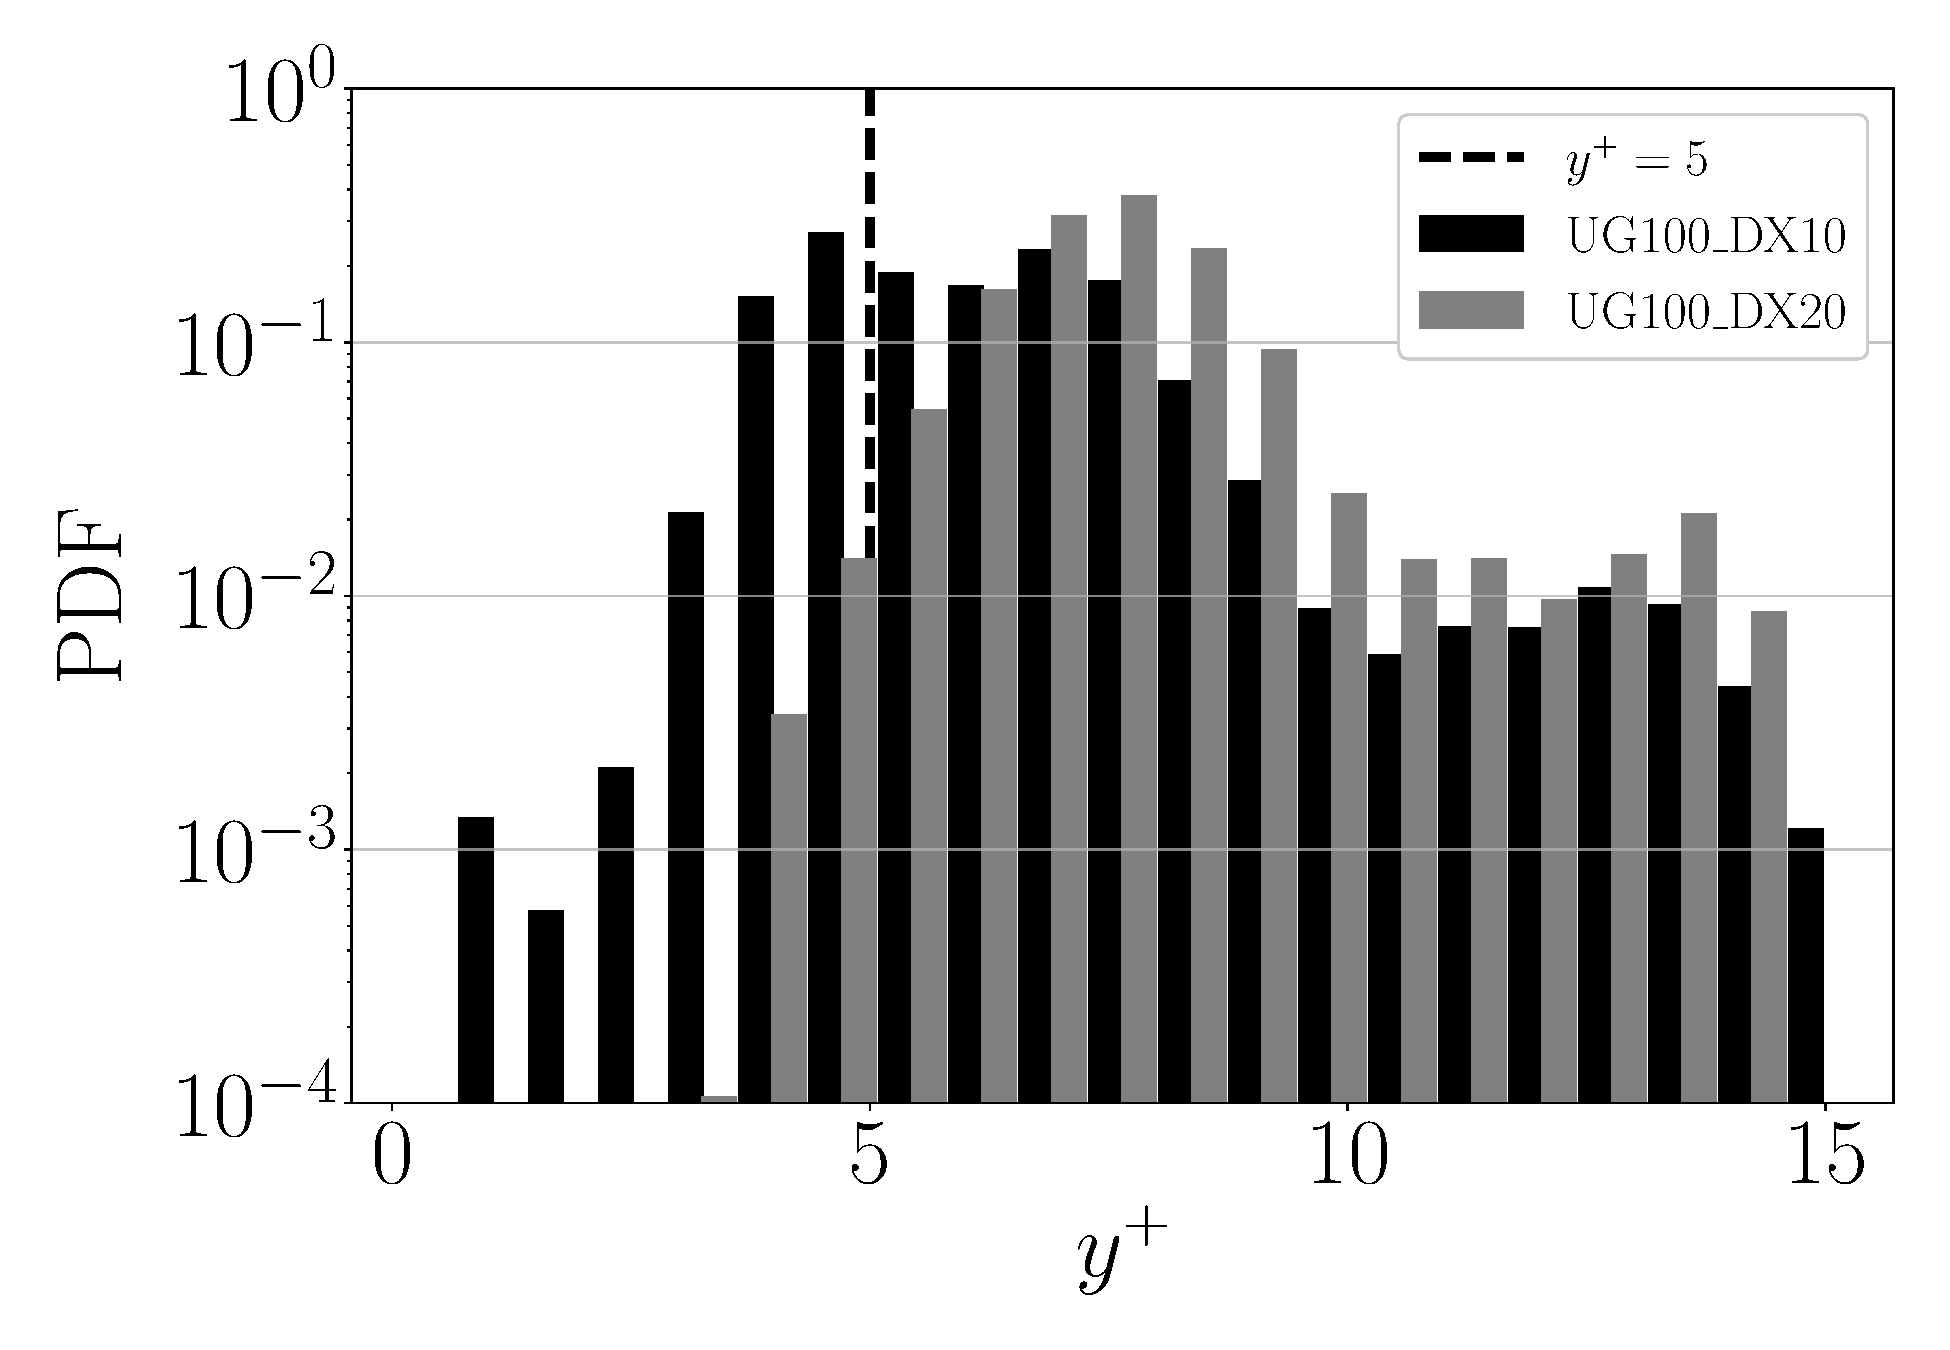
\includegraphics[scale=0.20]{./part2_developments/figures_ch5_resolved_JICF/instabilities_resolution/y_plus_injector}
   \vspace{-0.15in}
   \caption{PDF of $y^+$ at the nozzle walls for high Weber cases}
   \label{fig:jicf_nozzle_y_plus_PDF}
\end{figure}



%Besides a better resolution at the wall, the cells inside the injector far from the walls which are also comprised within the levelset band are also refined to the $\Delta x_\mathrm{min}$ value imposed.  

A cut on the $y = 0$ plane with a view on the nozzle region is displayed in Figure \ref{fig:jicf_injector_resolution_with_mesh}.  For $x < 0$ the element size field $\Delta x$ in the fine resolution simulation is shown, while the coarse one is displayed for $x > 0$. The interface outside the injector is highlighted by the white contour, and the band limits are denoted by the black contour. The metric within the band is smaller for the fine resolution, which is straightforward since this is the region with imposed $\Delta x_\mathrm{min}$. The band attaches inside the injector and refines the wall in this region, producing a better wall resolution for the fine simulation as it was shown in Figure \ref{fig:injector_visualization_y_plus}. Below the band reattachment location, the nozzle walls are not refined but the rest of the injector is, due to the transition from the cell size $\Delta x_\mathrm{min}$ to the baseline cell size (see Figure \ref{fig:AMR_strategy}). The refinement is found to extend upstream the straight section of the injector: the fine simulation contains smaller elements that the coarse one in this region, while both meshes then show similar element sizes in the tapered section of the nozzle as shown by the zoomed-in region of Figure \ref{fig:jicf_injector_resolution_with_mesh}.




The improved resolution inside the last section of the nozzle as shown by Figure \ref{fig:jicf_injector_resolution_with_mesh} might have an impact on the development of turbulence in this region. Further insight is given in Figure \ref{fig:jicf_nozzle_disks}, where $TKE$ is displayed in two planes perpendicular to the flow direction at two vertical locations: $z = -0.35$ mm (in the middle of the injector, outside the levelset band refined region) and $z = 0$ mm (the nozzle exit, where cells are refined within the levelset band). The $TKE$ values are low at the center of the injector and high around the walls: in fact, the liquid Reynolds numbers $Re_l$ in the operating points considered (see Table \ref{tab:jicf_operating_conditions}) indicate laminar flow within the injector, hence the freestream liquid flow does not transition into a turbulent state and the turbulent content is null at the center of the injector. $TKE$ increases then at the walls due to the presence of the boundary layer. As observed in Figure \ref{fig:jicf_nozzle_disks}, the coarse case displays low values of $TKE$ with respect to the fine simulation, where $TKE \sim 1$ closer to the walls around all its azimuthal perimeter. The differences in the turbulent state are seen both at $z = 0$ mm and at $z = -0.35$ mm due to the nozzle refinement from the levelset band location up to the tapered section.


\begin{figure}[ht]
	\centering
   \includegraphics[scale=0.28]{./part2_developments/figures_ch5_resolved_JICF/instabilities_resolution/injector_resolution_with_mesh}
   \caption{Mesh element size $\Delta x$ shown at plane $y = 0$ for instantaneous simulations of cases UG100\_DX10, UG100\_DX20}
   \label{fig:jicf_injector_resolution_with_mesh}
\end{figure}

\clearpage

\begin{figure}[ht]
	\centering
   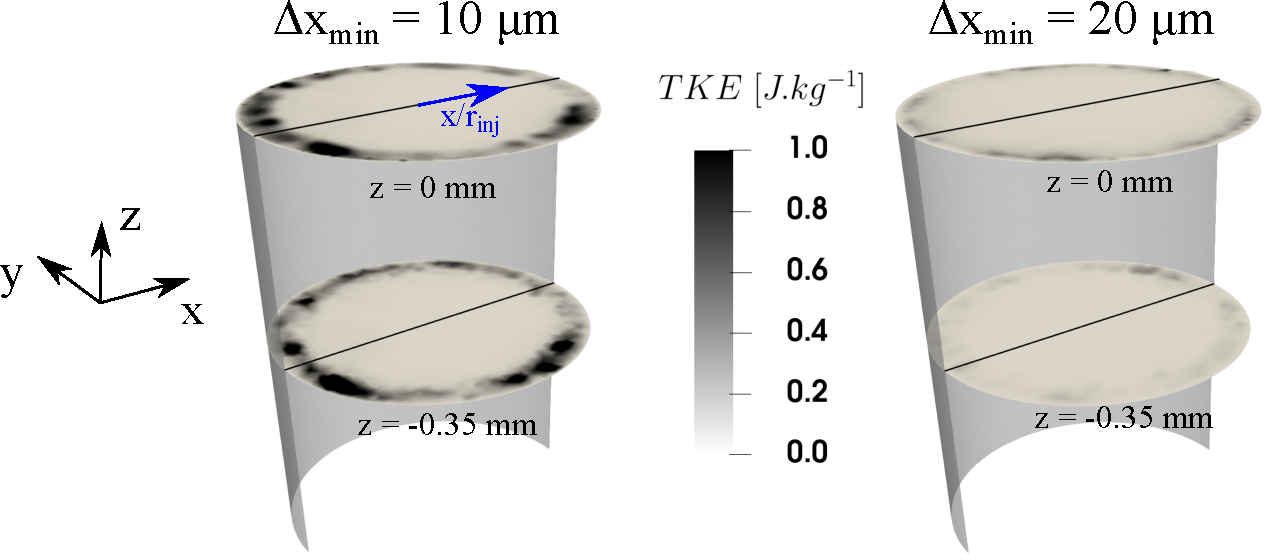
\includegraphics[scale=0.5]{./part2_developments/figures_ch5_resolved_JICF/instabilities_resolution/injector_visualization_disks}
   \vspace*{-0.1in}
   \caption{Planes within the injector showing TKE at locations $z = 0, -0.35$ mm for the high Weber case}
   \label{fig:jicf_nozzle_disks}
\end{figure}


The profiles of mean vertical velocity $\overline{w}$, $TKE$ and mean vorticity magnitude $|\overline{\omega}|$ obtained at the black lines from Figure \ref{fig:jicf_nozzle_disks} are plotted in Figure \ref{fig:jicf_data_lines_inside_injector}. Due to symmetry, only the first half has been shown. The boundary layer thicknesses $\delta$ are obtained as the points where $\overline{w}$ decrease to $99~\%$ of its value at the center ($x = 0$ mm). The $\overline{w}$ graph shows that $\delta$ and velocity profiles depend on the resolution $\Delta x_\mathrm{min}$ employed: the fine case shows a thinner boundary layer and a steeper $\overline{w}$ profile, specially at $z = 0$ mm. Both $TKE$ and $|\overline{\omega}|$ profiles show higher contents within the boundary layer in the fine case: in the case of $TKE$, case UG100\_DX20 shows a peak of $0.2~J.kg^{-1}$ magnitude while case UG100\_DX10 retrieves $0.57~J.kg^{-1}$, which is almost three times larger. This higher liquid turbulent state within the injector for the fine resolution could cause the initial interface perturbations that develop into the surface instabilities observed in the fine case. Nevertheless, it is not clear whether the differences in the turbulent state are significant to trigger instabilities: even though there is a ratio of 3 between the maximum $TKE$ found among resolutions, the relation $TKE/ \left( 0.5 u_l^2 \right)$ (i.e. TKE againt bulk liquid kinetic energy) is of $0.075~\%$ for UG100\_DX20 and of $0.2~\%$ for UG100\_DX10, while turbulent liquid jets where the turbulence within the injector is thought to create the instabilities \citepColor[xiao_large_2013] yield ratios of the order of $TKE/ \left( 0.5 u_l^2 \right) \sim 2 \%$ \citepColor[tretola_effect_2021]. The ratio TKE - bulk kinetic energy found in this work is one order of magnitudes lower than the ratios reported in literature: this could mean that liquid turbulent fluctuations do not reach the threshold level to overcome surface tension forces, meaning that they would not be the cause of the instabilities \citepColor[lee_primary_2007]. Nevertheless, this TKE threshold is not known (more research would be needed to ellucidate this value, as literature on the topic is scarce to the knowledge of the author) and such conclusion cannot be drawn from the analysis here presented.


\begin{figure}[ht]
\flushleft
\begin{subfigure}[b]{0.3\textwidth}
	\flushleft
   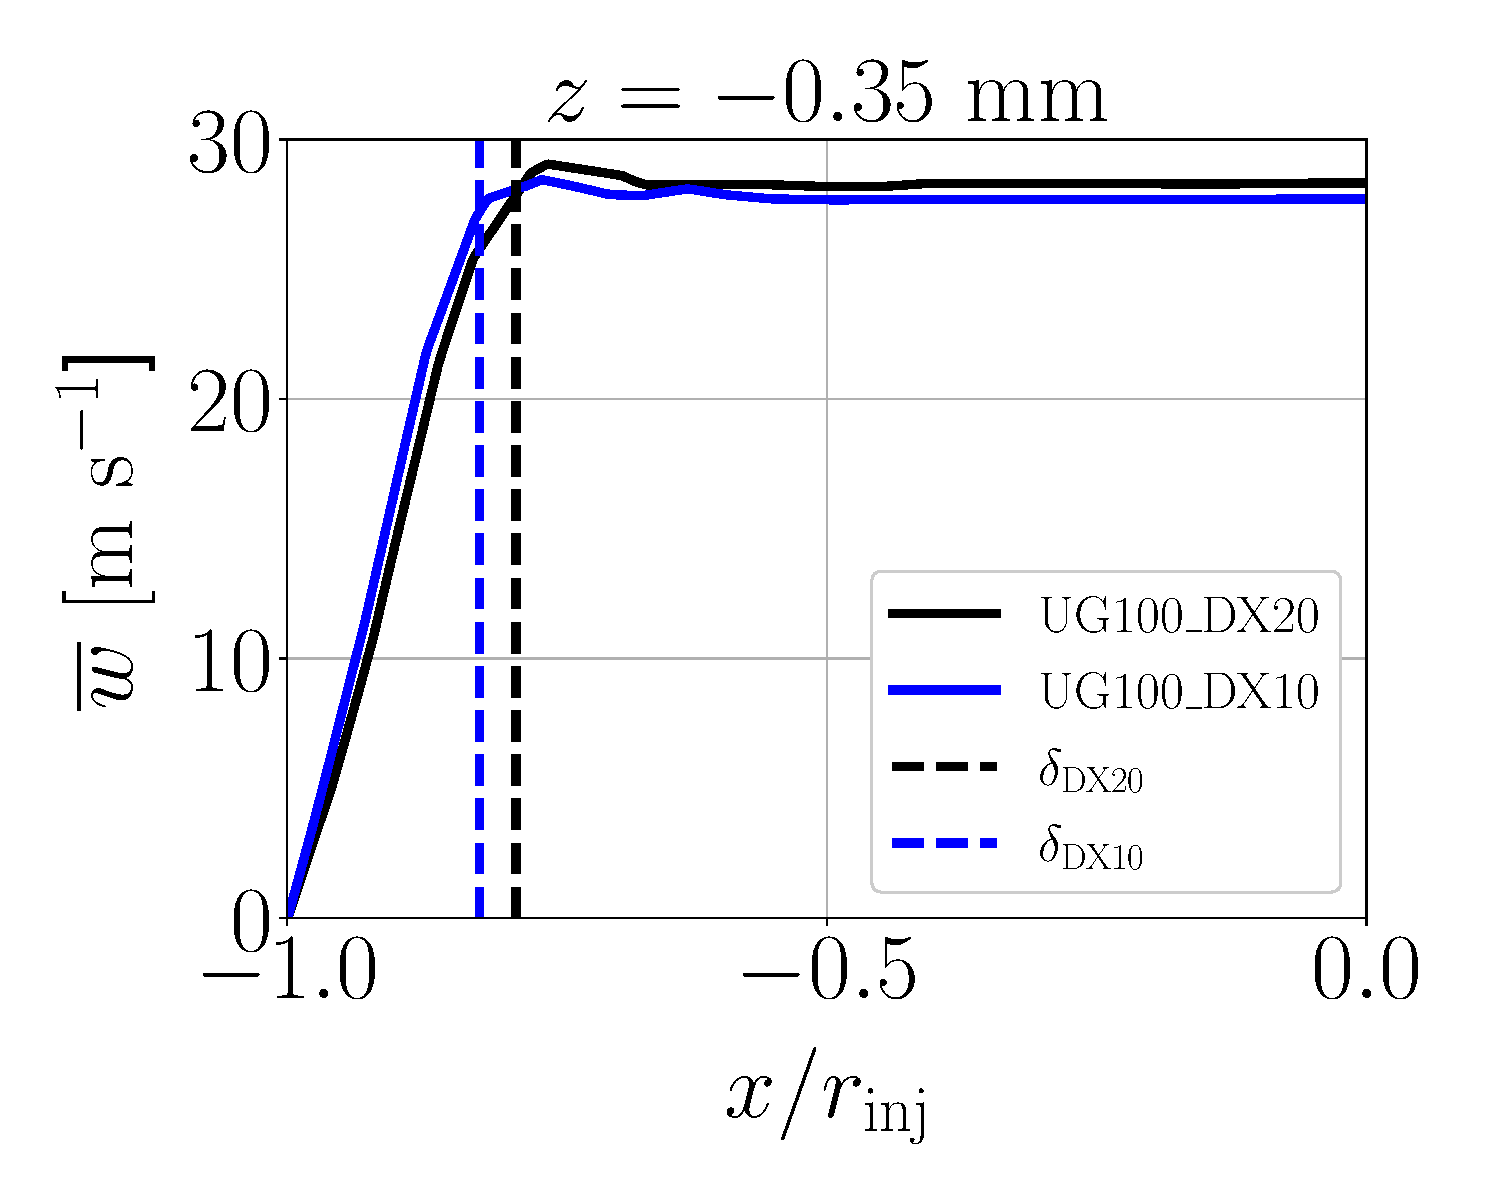
\includegraphics[scale=0.225]{./part2_developments/figures_ch5_resolved_JICF/instabilities_resolution/line_data_injector_uz_zm0p35}
\end{subfigure}
\hfill
\begin{subfigure}[b]{0.3\textwidth}
	\flushleft
   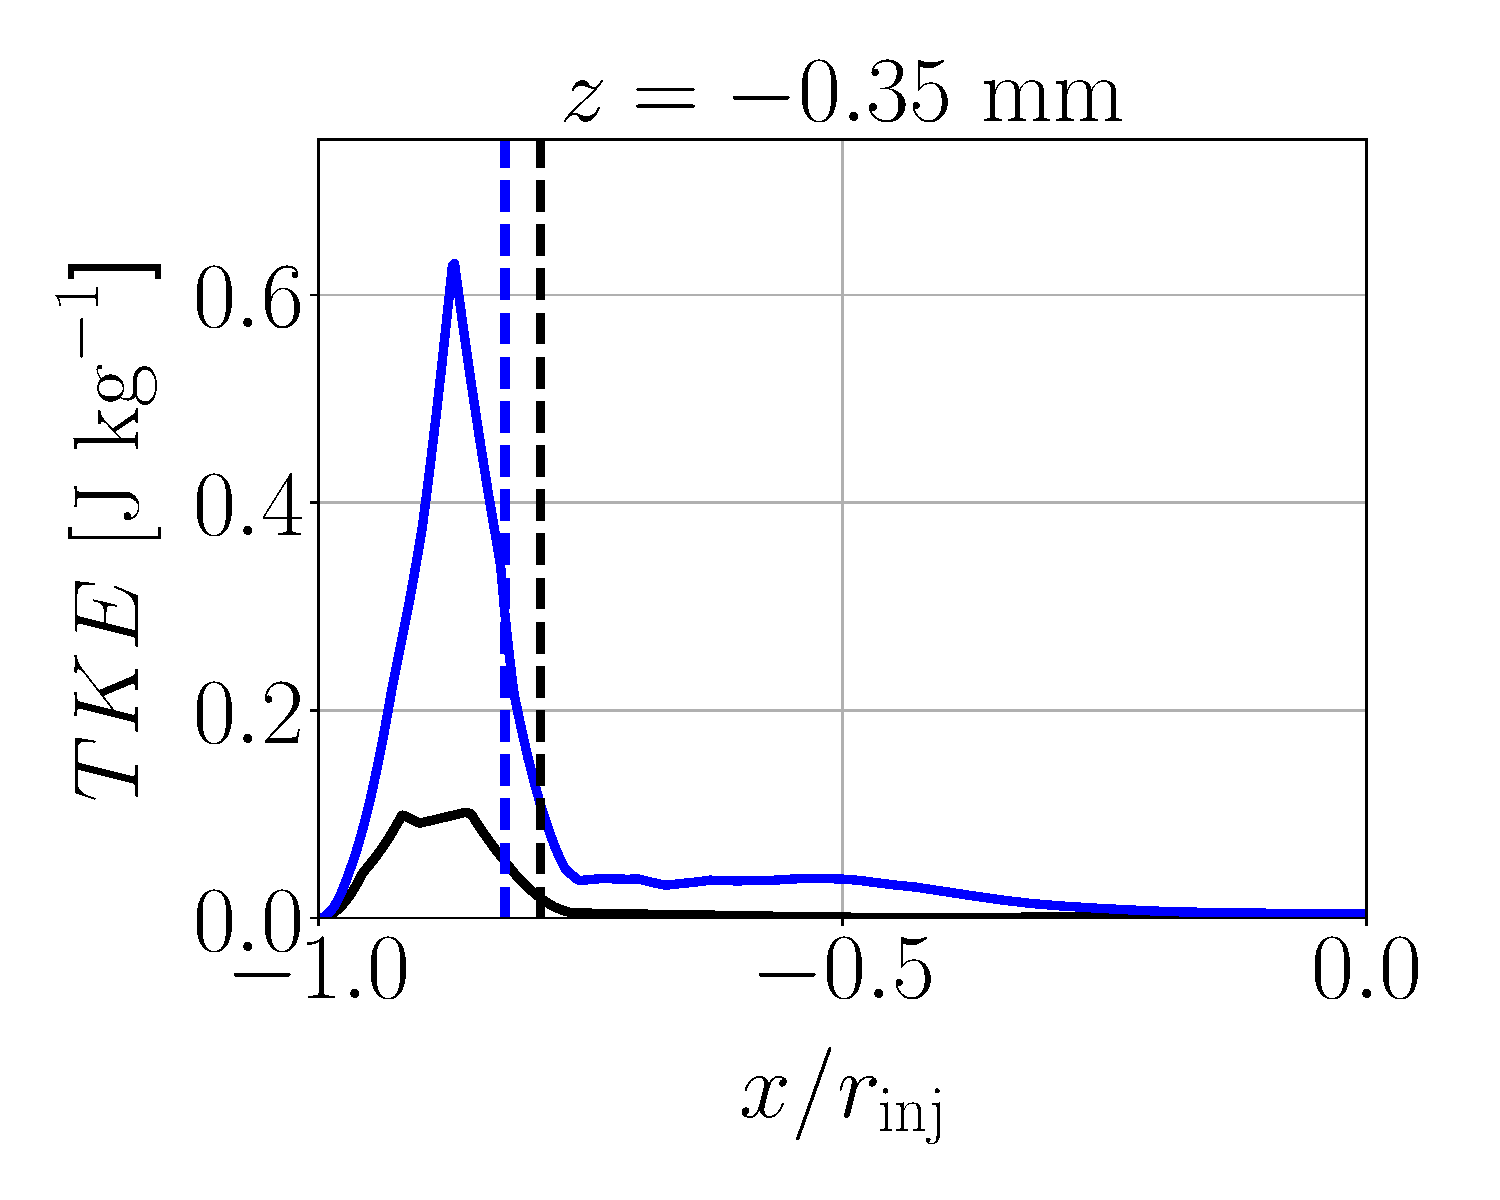
\includegraphics[scale=0.225]{./part2_developments/figures_ch5_resolved_JICF/instabilities_resolution/line_data_injector_TKE_zm0p35}
\end{subfigure}
\hfill
\begin{subfigure}[b]{0.3\textwidth}
	\flushleft
   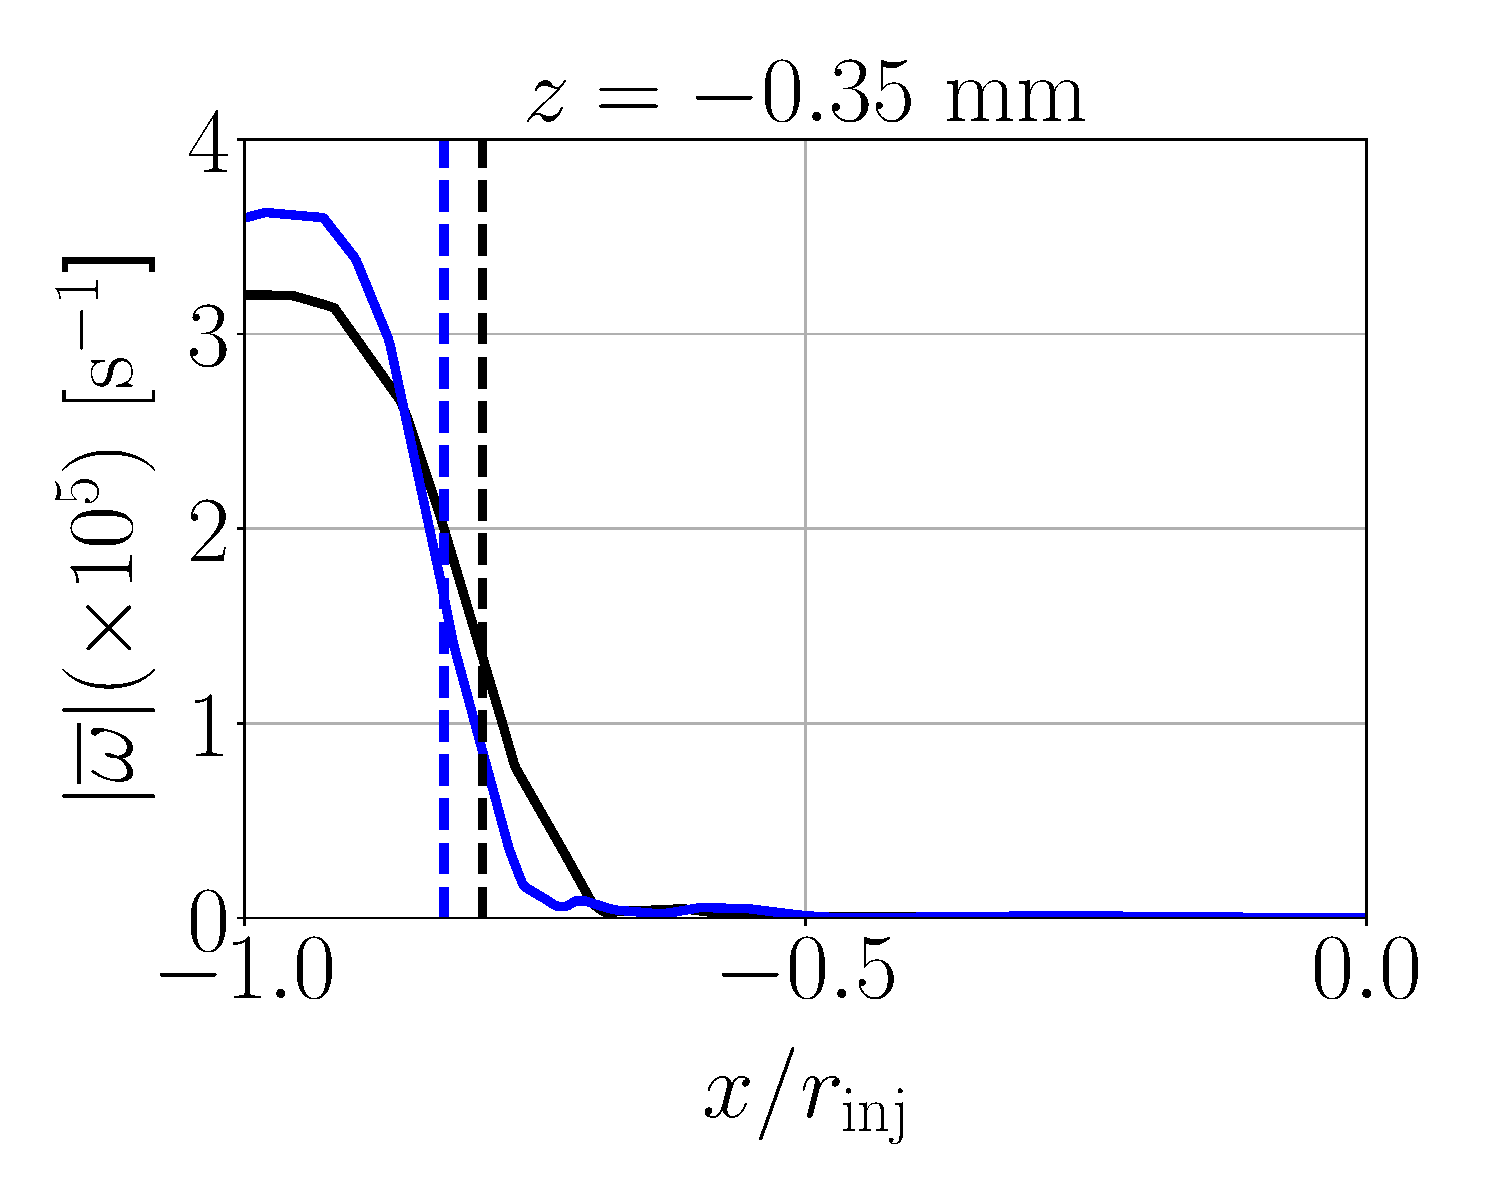
\includegraphics[scale=0.225]{./part2_developments/figures_ch5_resolved_JICF/instabilities_resolution/line_data_injector_vort_zm0p35}
\end{subfigure}

\vskip\baselineskip
\vspace*{-0.6in}

\begin{subfigure}[b]{0.3\textwidth}
	\flushleft
   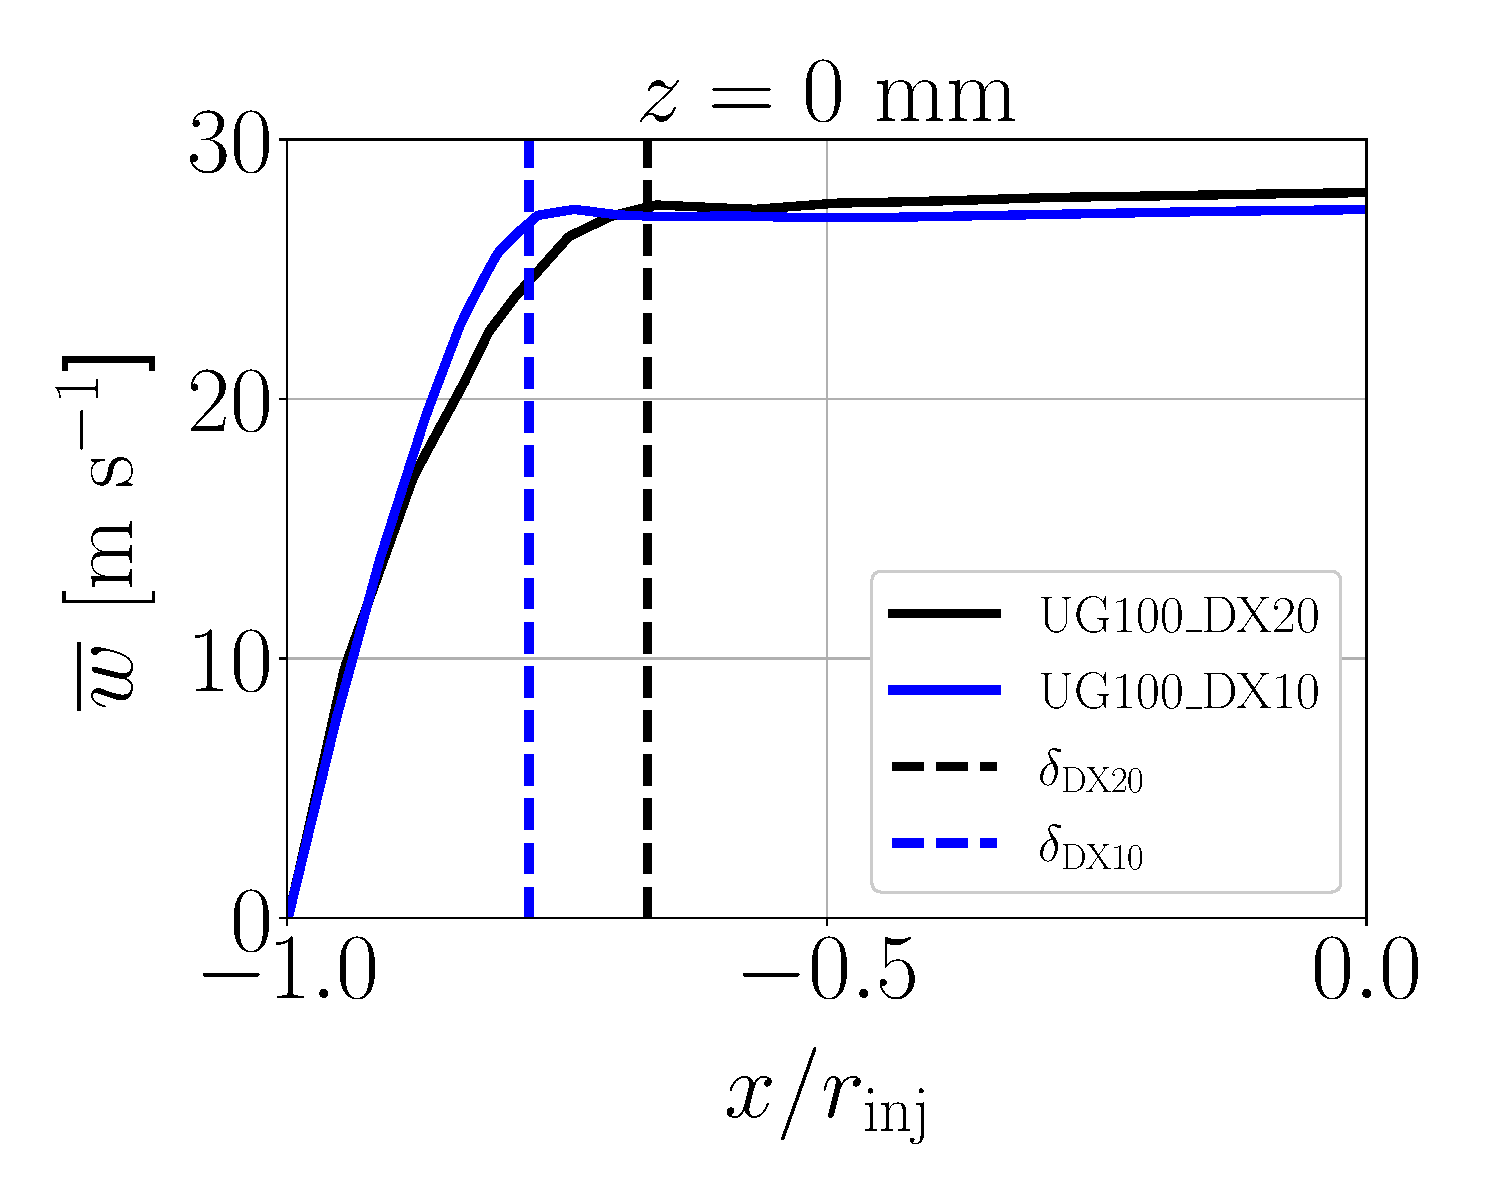
\includegraphics[scale=0.225]{./part2_developments/figures_ch5_resolved_JICF/instabilities_resolution/line_data_injector_uz_z0p00}
\end{subfigure}
\hfill
\begin{subfigure}[b]{0.3\textwidth}
	\flushleft
   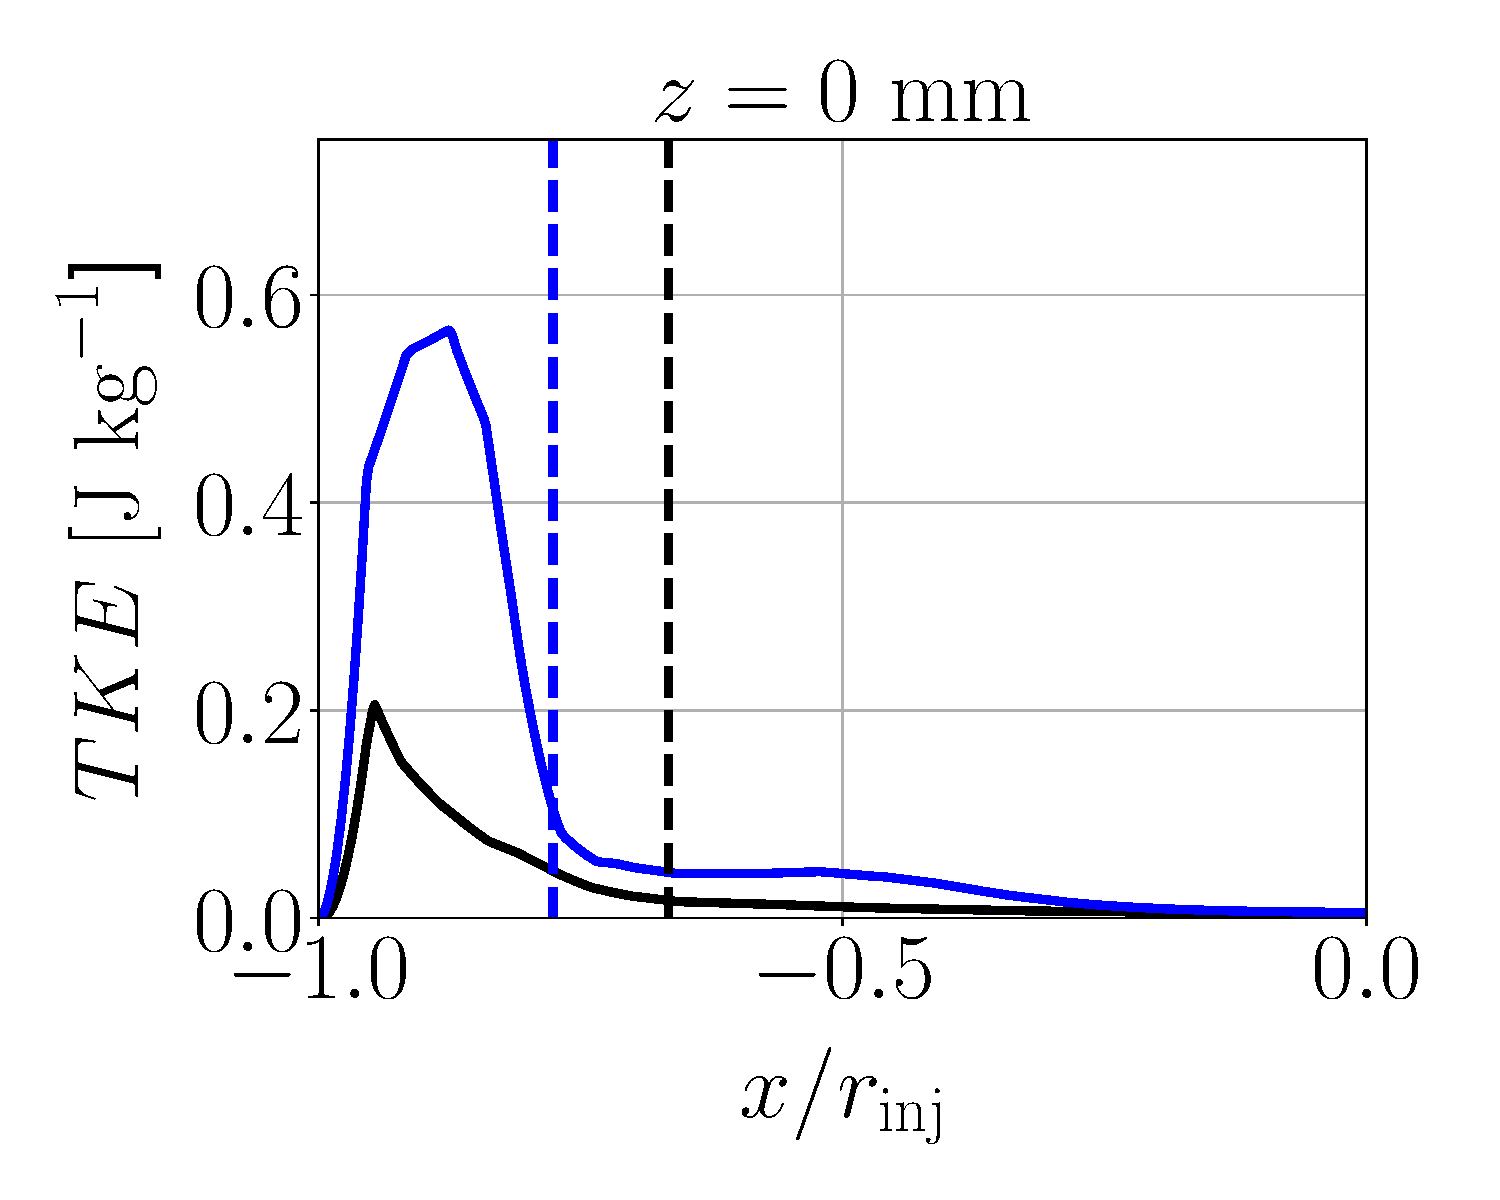
\includegraphics[scale=0.225]{./part2_developments/figures_ch5_resolved_JICF/instabilities_resolution/line_data_injector_TKE_z0p00}
\end{subfigure}
\hfill
\begin{subfigure}[b]{0.3\textwidth}
	\flushleft
   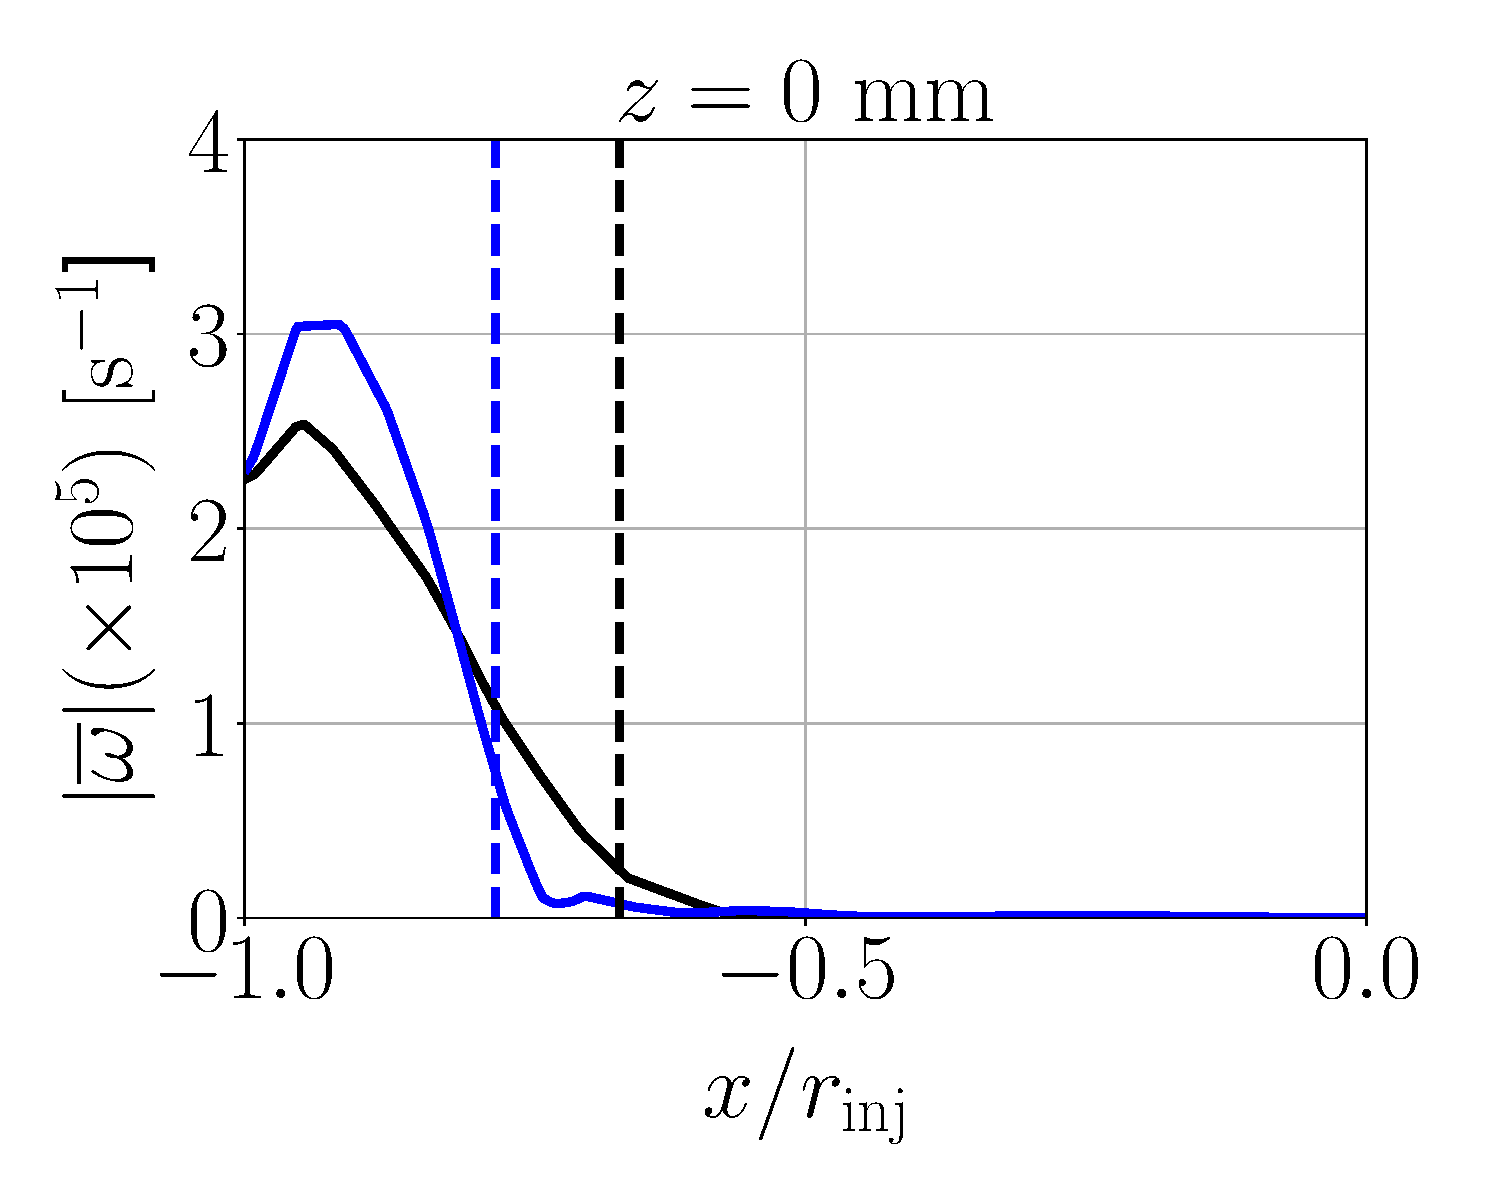
\includegraphics[scale=0.225]{./part2_developments/figures_ch5_resolved_JICF/instabilities_resolution/line_data_injector_vort_z0p00}
\end{subfigure}

   \vspace*{-0.15in}
   \caption{Profiles of mean vertical velocity, $TKE$ and mean vorticity magnitude at lines located at $y = 0$ along the planes $z = -0.35,~0$ mm}
\label{fig:jicf_data_lines_inside_injector}
\end{figure}

\clearpage

\subsubsection*{3) Gaseous field perturbed by the jet}


%\textbf{Ver tambien refs: 2013-Xiao, 2020-zhou, 2017-zhanng}

The third hypothesis on instabilities is that a finer cell size resolves better the gaseous field perturbed at the vicinity of the liquid interface. Indeed, the liquid conditions within the injector are laminar, and \citeColor[xiao_large_2013] suggested that for laminar jets the liquid turbulence does not play a paramount role (while it does for turbulent liquid conditions) and instabilities are instead triggered by shear caused by the incoming gaseous crossflow. The influences of the interface mesh resolution $\Delta x_\mathrm{min}$ on the gas phase are then examined in the following lines.



%Another hypothesis is that the gaseous phases are different near the injector zone, since there is a growth in element size from the interface cell size $\Delta x_\mathrm{min}$ to the baseline mesh, and therefore the cells in the fine resolution located at the vicinity of the interface are also finer. This hypothesis is tested by looking at the vorticity $\omega = \frac{1}{2} \left( \nabla \times \textbf{u} \right)$ in 

Instantaneous view of the jets and plane $y = 0$ mm from cases UG100\_DX10 and UG100\_DX20 colored by the vorticity magnitude are shown in Figure \ref{fig:JICF_instabilities_vorticity}. The fine jet shows high vorticity regions along the interface due to the instabilities formed, as well as high vorticity in the bottom part of the jet at the windward side, which indicates the onset of the instabilities. The coarse jet does not display relevant vortical structures in the jet until column breakup starts taking place downstream the injection point. The zoomed-in views of the plane $y = 0$ close to the wall shows the streamlines and vorticity distribution in the gaseous field upstream the jet. Gaseous vorticity around the interface is much higher for the fine case: roll-up vortices, which are not seen in the coarse simulation, appear and disturb the interface, amplifying the instabilities (they might even be their cause, even though this cannot be fully ensured in this analysis). Horseshoe vortices, englobed by dashed red circles, are also observed at the wall upstream upstream the liquid injector. This vortex, which is a common feature in both gaseous \citemColor[kelso_experimental_1996,zhang_flow_2017] and liquid \citepColor[zhou_simulation_2020] JICF, is stronger for the coarse simulation and weaker for the fine one (despite the mesh at its location being identical in both simulations), even though it seems not to impose a significant perturbation on the gaseous streamlines, which are on the other hand perturbed by the roll-up vortices.


\begin{figure}[ht]
\flushleft
\includeinkscape[inkscapelatex=false,scale=0.75]{./part2_developments/figures_ch5_resolved_JICF/instabilities_resolution/JICF_instabilities_vorticity}
\caption[Instantaneous vorticity fields for the high Weber operating point.]{Instantaneous vorticity fields for the high Weber operating point. Streamlines are shown in the zoomed-in regions}
\label{fig:JICF_instabilities_vorticity}
\end{figure}

The vertical velotity profiles along the yellow lines $z = 0.05, 0.2$ mm represented in Figure \ref{fig:JICF_instabilities_vorticity} are shown in Figure \ref{fig:jicf_data_lines_outside_injector}. The lines span along the $x$ direction but a change of coordinate has been done to the axial coordinate $s = x - x_\mathrm{int}$, where $x_\mathrm{int}$ is the location of the interface. Closer to the wall ($z = 0.05$ mm), the $w$ profile shows slight differences among resolutions in the vicinity of the interface: the fine case retrieves higher velocity peaks in the liquid and gaseous regions, but still very close to the coarse one. In the liquid region ($s > 0$) the fine simulation reaches faster the freestrem liquid velocity than the coarse one due to a thinner, better resolved boundary layer than in the coarse simulation. In the gaseous phase the velocity profiles are distinct due to the different perturbation of the streamlines as shown in Figure \ref{fig:JICF_instabilities_vorticity}: the fine case shows negative velocities until reaching the farfield value $w = 0$, while the coarse one presents negative values larger in absolute value than the fine case up to $s \sim -0.15$ mm and then sees a increase to positive values due to the higher perturbation induced by the stronger horseshoe vortex. When looking further from the wall, at $z = 0.2$ mm, the profiles show similar behaviour within the liquid region but significant differences in the gaseous phase: for the fine resolution, the vertical velocity drops quickly with decreasing $s$ from its interface value to below $w = - 20$ m s$^{-1}$ and then relatex towards a freestream value close to 0, while the coarse one shows a less sharp gradient. The sharp gradient in the fine case is a possible source of shear force around the interface which can contribute to the development and amplification of the instabilities. Nevertheless, it is yet not clear whether this gradient is the cause of the instabilities, or it is actually caused by other factors such as the turbulence developed within the injector.

\clearpage


\begin{figure}[ht]
\flushleft
\begin{subfigure}[b]{0.45\textwidth}
	\flushleft
   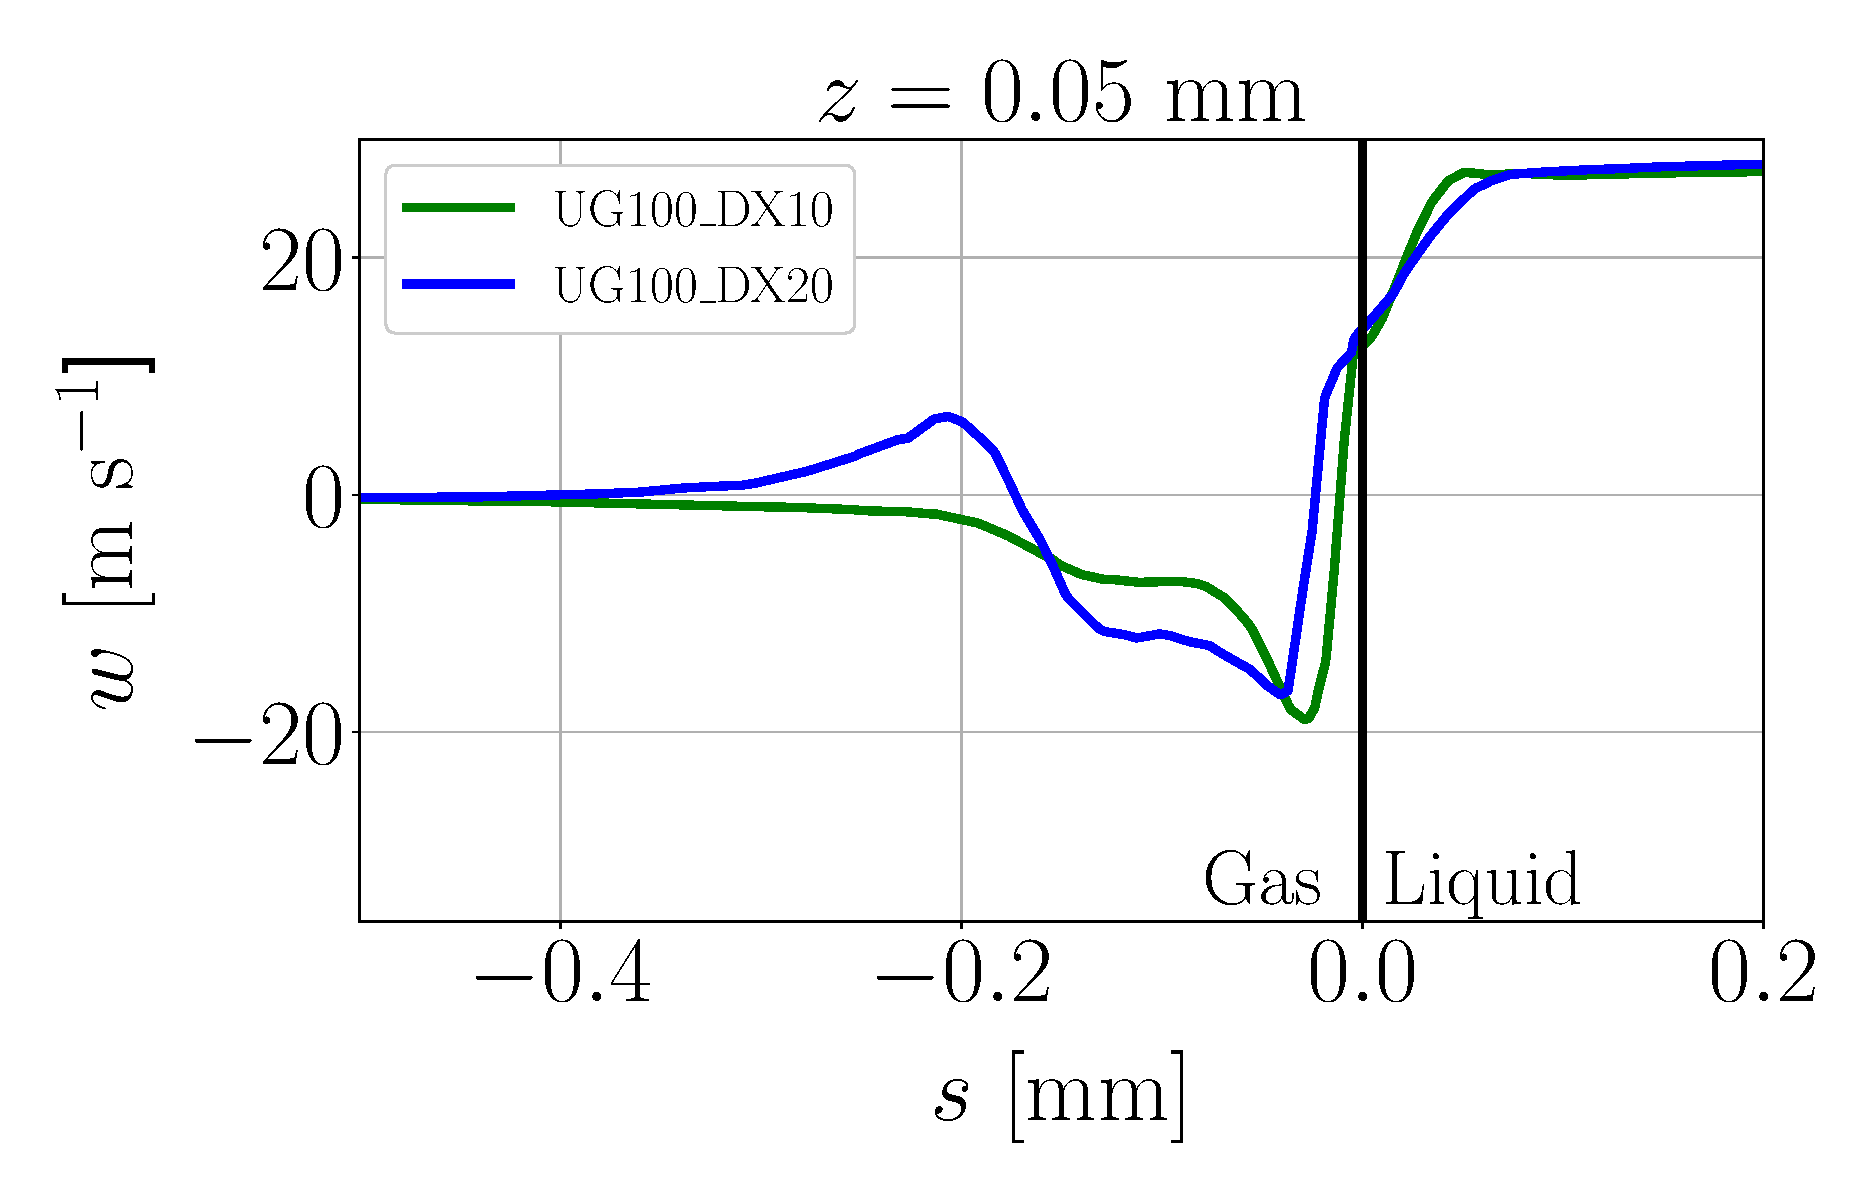
\includegraphics[scale=0.25]{./part2_developments/figures_ch5_resolved_JICF/instabilities_resolution/line_data_outside_injector_z_low}
\end{subfigure}
\hfill
\begin{subfigure}[b]{0.45\textwidth}
	\flushleft
   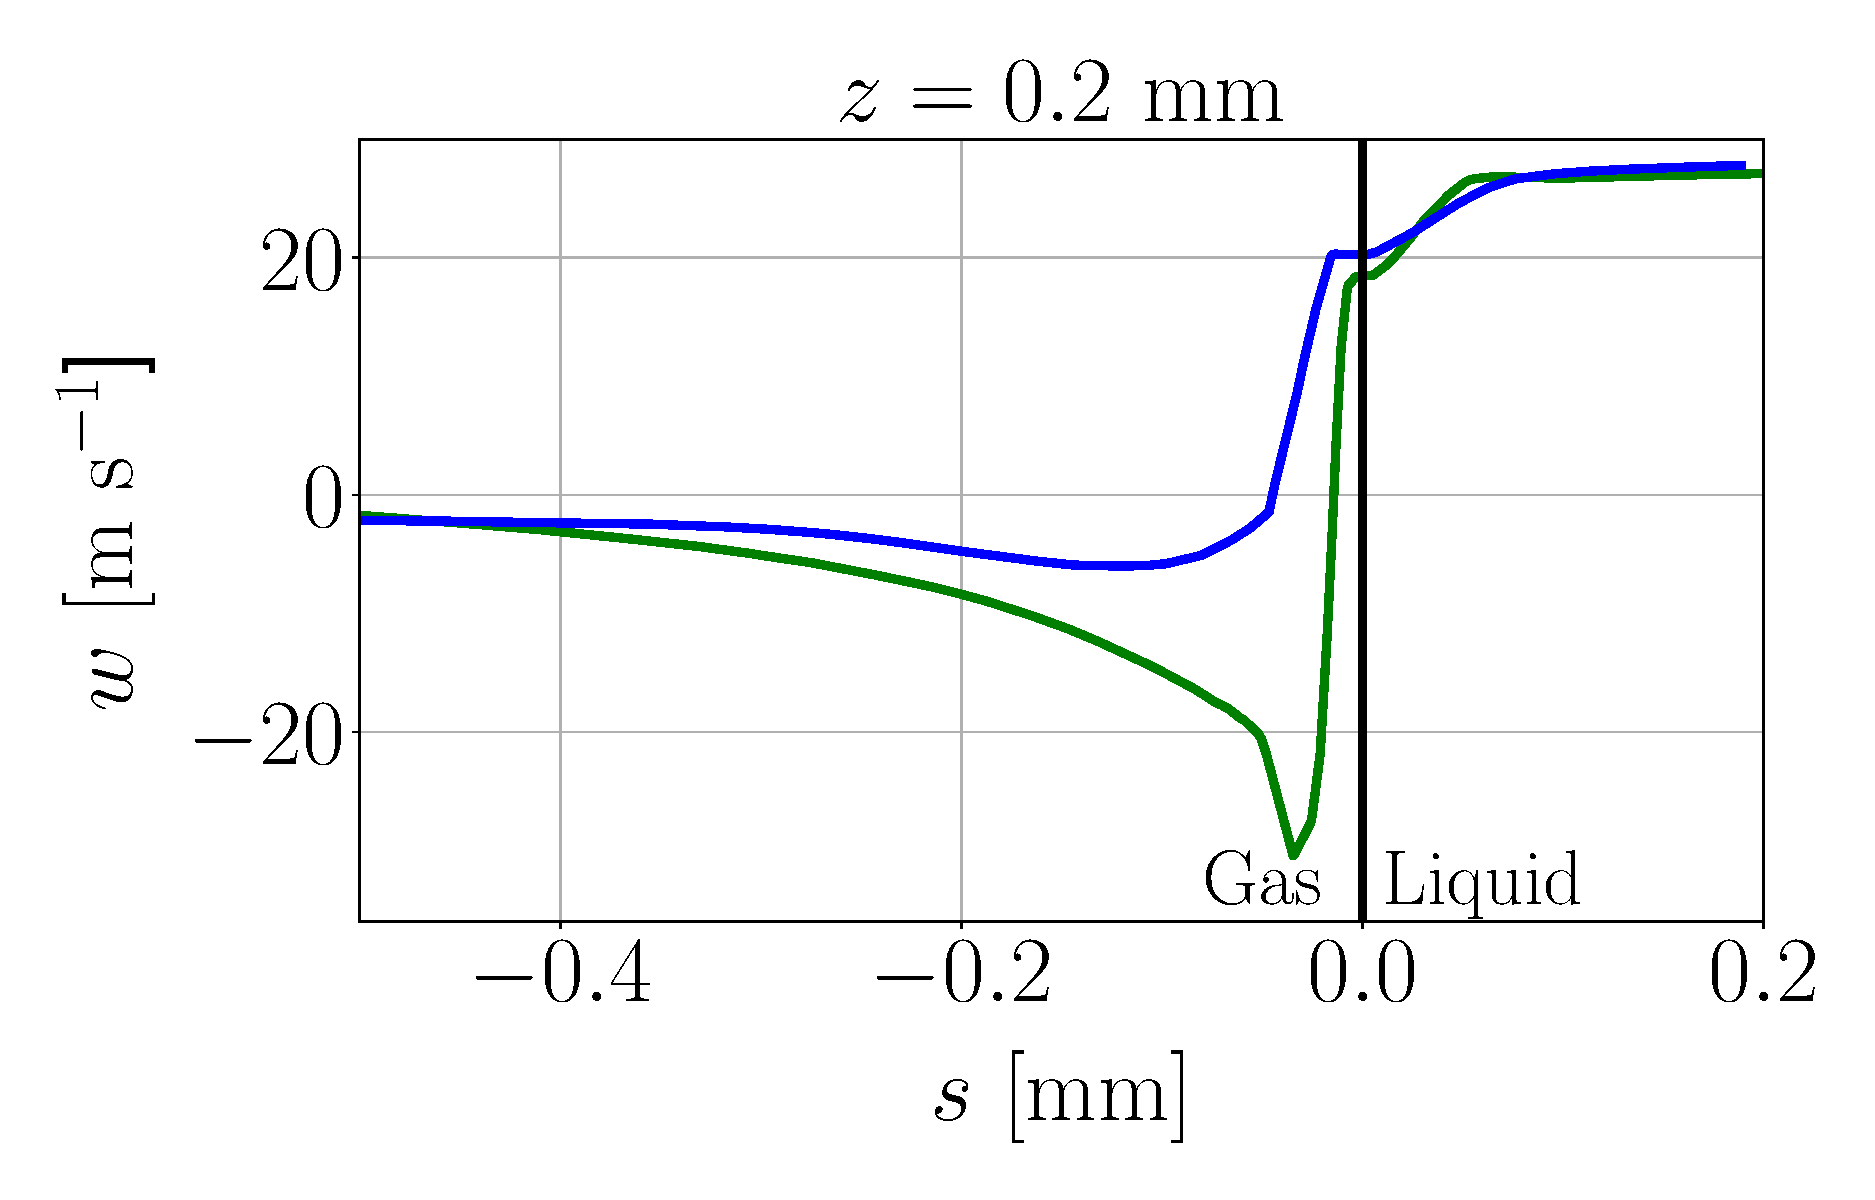
\includegraphics[scale=0.25]{./part2_developments/figures_ch5_resolved_JICF/instabilities_resolution/line_data_outside_injector_z_upper}
\end{subfigure}

   \caption[Vertical velocity profiles at yellow lines depicted in Figure \ref{fig:JICF_instabilities_vorticity}]{Vertical velocity profiles at yellow lines depicted in Figure \ref{fig:JICF_instabilities_vorticity}. The black vertical line indicates the location of the interface: negative $s$ values are located in the gas phase while positive ones are in the liquid phase}
\label{fig:jicf_data_lines_outside_injector}
\end{figure}

From the analysis performed in this section, it can be stated that refining the mesh at the interface has an effect on both the liquid phase within the injector and the gaseous phase upstream the injection point. Differences have been observed in the liquid nozzle, particularly in relation to the resolution of the boundary layer in the injector walls and the turbulent magnitudes $TKE$ and vorticity: nevertheless, the differences might not be significant in absolute values to be the cause of the instabilities. A proper assessment of this statement should be done by comparing the obtained values with reference values from studies dealing with similar configurations and operating conditions, which are not present in literature nowadays to the knowledge of the authors. Observation of the gaseous phase has shown relevant differences among interface resolutions, particularly in relation to the appearance of vortical structures and shear layers around the interface which are directly linked to interfacial instabilities. However, it is not clear if these features in the gaseous field are the cause of the early development of the instabilities or a consequence of them: this one has been a fundamental question in the field of jets open for a long time \citepColor[rayleigh_instability_1878] which requires further study. %Further studies would require to analyze both hypothesis separately, something which has not been 




%As observed in Figure \textbf{XX}, ligaments generated due to instabilities in the fine resolution simulations \hl{contain a higher inertia and are stripped-off the dense core with larger velocities than those produced in the coarse resolution, where instabilities are not generated}. Such ligaments and the subsequent droplets produced from their breakup will penetrate further away in the vertical direction.

%We can see in Figure \textbf{XX} that the wavelengths $\lambda$ of the generated instabilities are ...

%When instabilities are present, primary atomization is affected and the generated ligaments \hl{contain more inertia}. As




\subsection{Jet trajectories}
\label{subsec:ch5_jet_trajectories_results}

One of the most important characteristics of a jet in crossflow is its vertical trajectory (see $\S$\ref{sec:ch1_fuel_injection_technology}). This feature determines how far the jet penetrates into the chamber, and has a paramount effect on the latter evaporation and mixing processes, hence affecting flame dynamics in reactive cases. Experimental studies often provide correlations for the trajectory of the windward side of the jet (see Table \ref{tab:correlations_experimental_JICF}). This is the side indicating the furthest vertical location ($z$) containing liquid for each axial location in crossflow direction ($x$). %Correlations relating $z$ and $x$ are often specified for a specific operating range ($q$ and $We$ limits) and up to a certain axial location downstream the injection point. 

In this section, trajectories from the resolved simulations are analyzed and compared with an experimental correlation. Four post-processing methods for obtaining trajectories are applied to one computation for illustrating their differences. Finally, one method is selected (based on its similarity with the experimental processing methodologies) for comparing the trajectories among simulations. The four methodologies employed (which are thoroughly detailed in Appendix \ref{app:processing_JICF_trajectories}) are grouped into two different families, \textbf{mean trajectory methods} or \textbf{instantaneous trajectory methods}, according to whether they process the mean or instantaneous $\psi$ field respectively:

\begin{itemize}

	\item Methods based on processing and averaging \textbf{instantaneous trajectories} (hereafter referred as instantaneous methods). These retrieve, at each time instant, the windward contour of the jet by sweeping the $z$ axis and identifying the points with $\psi = 0.5$ at the plane $y = 0$. This provides an instantaneous trajectory per timestep, which can eventually be averaged to provide mean trajectories. If when sweeping the $z$ axis, only the points belonging to the outer profile are retrieved, the resulting trajectory is \textbf{monotonic}. If, on the other hand, points belonging to the inner structure of the jet are also sampled, then the trajectory is \textbf{non-monotonic}.
	
	\item Methods based on the \textbf{mean levelset function} ($\overline{\psi}$). On one hand, trajectories can be obtained as the contour defining the maximum gradient of the $\overline{\psi}$ field in the vertical direction for each axial coordinate: $\max \left( \nabla_z | \overline{\psi} | \right)$. On the other hand, trajectories can be directly obtained as an \textbf{iso-contour} of the $\overline{\psi}$ function, where the contour chosen in this work is $\overline{\psi} = 0.01$.

\end{itemize}

\clearpage

Table \ref{tab:jicf_tools_trajectories_obtention} summarizes the nomenclature for the four trajectories postprocessing methods.

\begin{table}[!h]
\centering
\caption{Summary of methods for computing JICF trajectories}
\begin{tabular}{ccc}
\thickhline
Group & Method & Nomenclature \\
\thickhline
\multirow{2}{*}{Instantaneous} & Non-monotonic & INST\_NM \\
 & Monotonic & INST\_M \\
 \hline
\multirow{2}{*}{Mean} & Maximum gradient & MEAN\_GRAD \\
 & Iso-contour & MEAN\_CONT \\
\thickhline
\end{tabular}
\label{tab:jicf_tools_trajectories_obtention}
\end{table}


%Different methods to obtain trajectories from resolved simulations were proposed in $\S$\ref{sec:ch5_tools_jicf_trajectories}. These methods are summarized in Table \ref{tab:jicf_tools_trajectories_obtention}. In this section, firstly  the four methods described are applied to the simulation UG100\_DX20, the trajectories obtained are then compared and discussed. Secondly, the method MEAN\_GRAD is chosen to perform experimental validation with all simulations from Table \ref{tab:jicf_resolved_simulations_performed}. \hl{Finally, a comparison of the $L_2$ errors based on the maximum distance downstream in the trajectory ...}


The trajectories obtained from the computations are also compared to the experimental correlation obtained by \citeColor[becker_breakup_2002], given by the following expression.:

\begin{equation}
    \label{eq:jicf_trajectory_becker}
    \frac{z}{d_\mathrm{inj}} = 1.57 \mathrm{q}^{0.36} \ln \left( 1 + 3.81 \frac{x}{d_\mathrm{inj}} \right)
\end{equation}

which is valid for $1 < q < 12$, $90 < We_\mathrm{ae} < 2120$ and $x/d_\mathrm{inj} < 22$. For the simulations studied, $d_\mathrm{inj} = 0.45$ mm and $q = 6$. The authors also present a standard deviation for the correlation of $\sigma = 0.81$. Numerical trajectories can be plotted together with Eq. (\ref{eq:jicf_trajectory_becker}) to provide a qualitative comparison of the computations. For further insight, a quantitative measure for the difference between simulations and experiments can be introduced through a $L_2$ norm:

\begin{equation}
\label{eq:L2_JICF}
    L_2 = \sqrt{\frac{1}{N}   \sum_{i=1}^N \left( \frac{z}{d_\mathrm{inj}} \Bigr|_{\mathrm{num},i} -   \frac{z}{d_\mathrm{inj}} \Bigr|_{\mathrm{exp},i} \right)^2}
\end{equation}

where $N$ is the number of points along the abscissa $x$ in which the difference between curves is evaluated and i refers to the $i$-th point. The subscript "num$,i$" indicates the mean value obtained from simulations for the vertical location at point $i$, while "exp$,i$" indicates the equivalent measure from experiments. From this definition it follows that the $L_2$ error is a measure of the deviation from experiments: the lower the $L_2$, the closer the simulation results are to the experimental ones. The $L_2$ error can also be monitored with time to determine the convergence evolution of the trajectories. \\

\paragraph*{Results}

In first place, the four methodologies are compared by applying them to simulation UG100\_DX20, since this is the one that has run for longer physical time. The resulting trajectories are shown in Figure \ref{fig:JICF_trajectories_and_L2_comparison}a. In the vicinity of the injector, all trajectories follow the same tendency up to $x/d_\mathrm{inj} \sim 1$. After this point, two different tendencies are observed: mean $\psi$ trajectories keep on following the experimental correlation, while instantaneous ones are located below. The different trends shown by the trajectories from both methodologies are due to their underlying definitions: instantaneous-averaged trajectories intend only to retrieve the outer contour of the jet, while the mean-based methods take the $\overline{\psi}$ field defined in all the domain and then obtain the trajectories at plane $y = 0$. The $\overline{\psi}$ field is diffused as opposed to the $\psi = 0.5$ contour retrieved by the instantaneous methods, so the trajectories obtained as $\max \left( \nabla_z | \overline{\psi} | \right)$ (maximum gradient) and $\overline{\psi} = 0.01$ (contour) are located in the regions where $\overline{\psi}$ is close to $0$ (i.e. where the mean presence of liquid is low). Consequently, trajectories penetrate further away than the instantaneous averaged ones in the near-injector region (coherent liquid) while they show the opposed tendency downstream after atomization has taken place (dispersed liquid) \\


\begin{figure}[ht]
\flushleft
\hspace{-0.5in}
\begin{subfigure}[b]{0.45\textwidth}
	\flushleft
   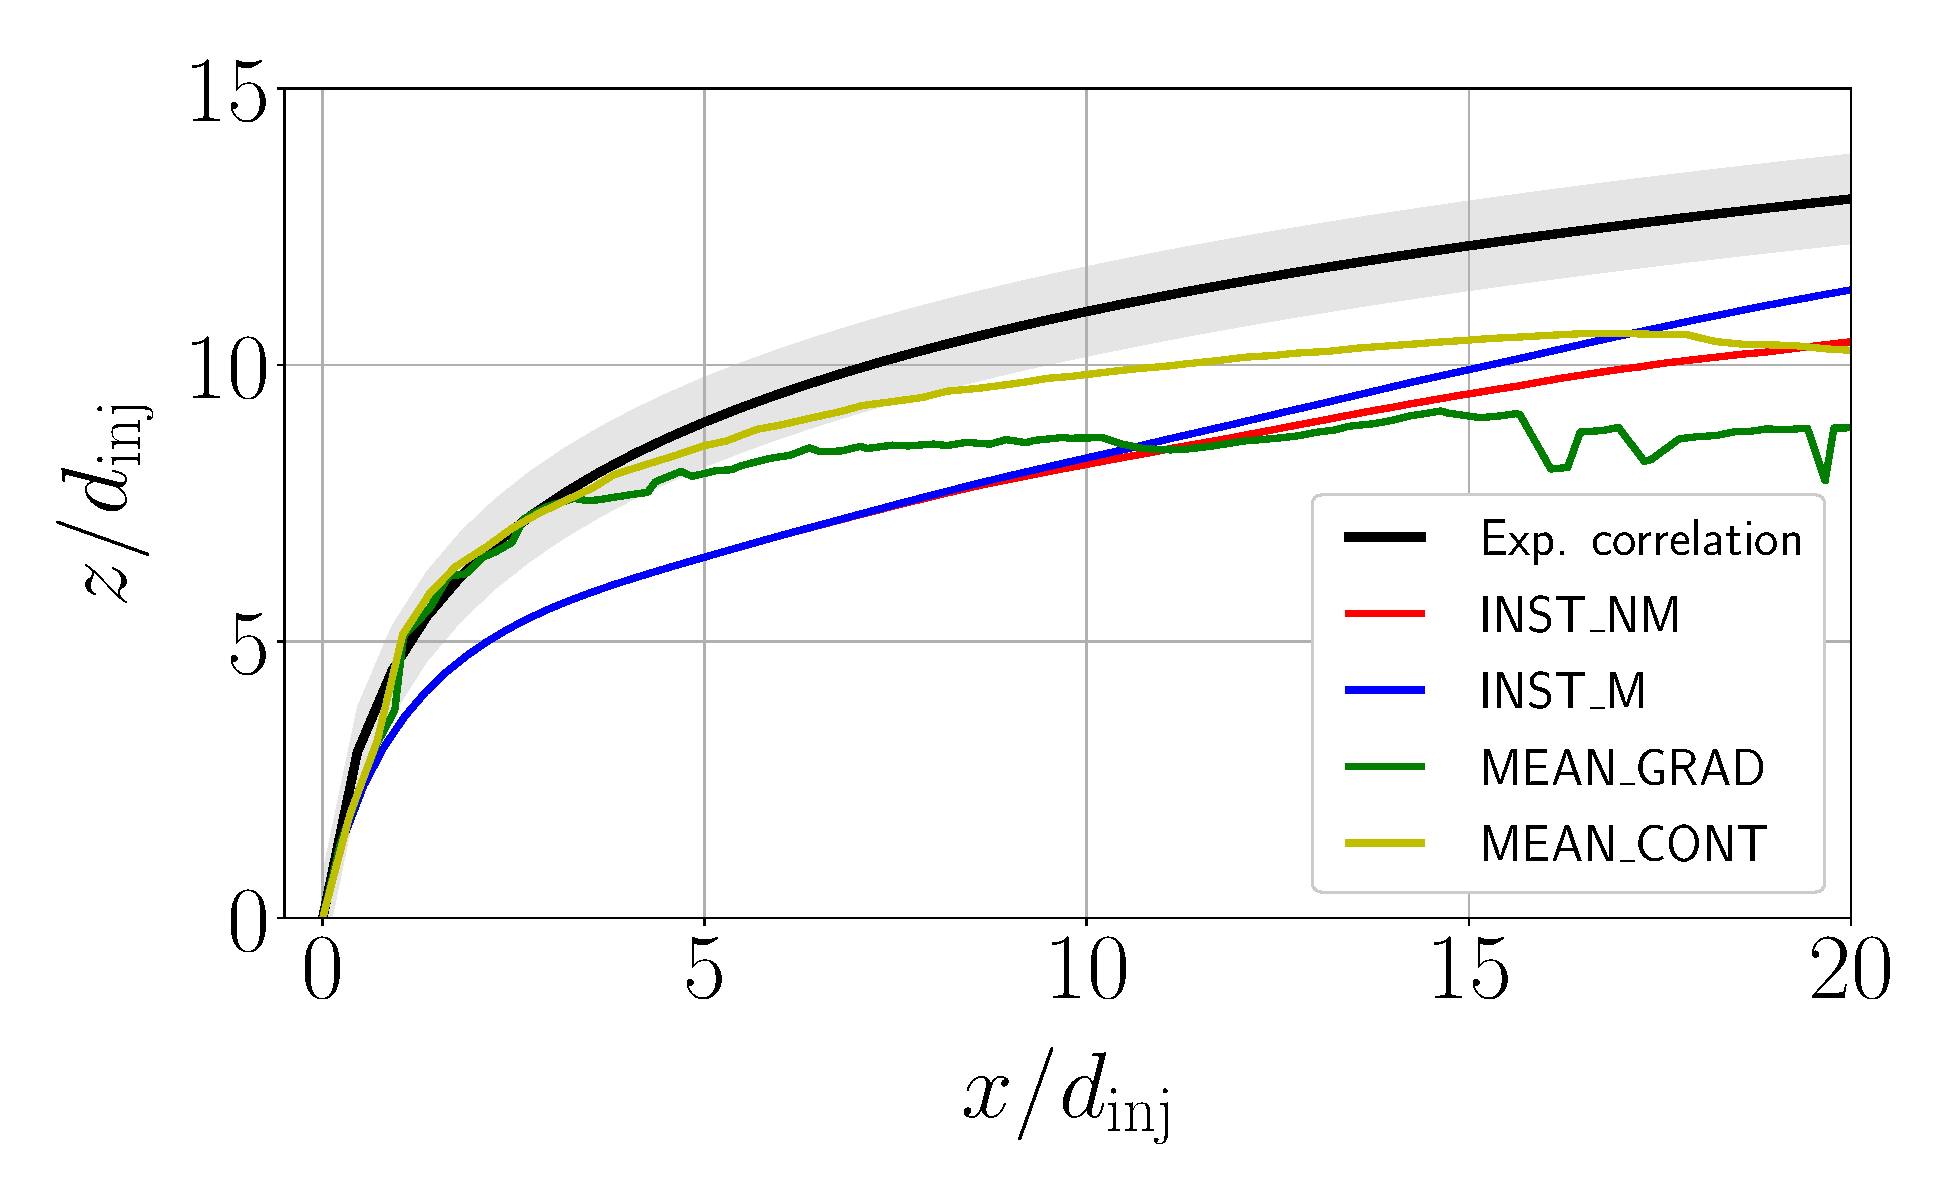
\includegraphics[scale=0.25]{./part2_developments/figures_ch5_resolved_JICF/results_trajectories/methods_comparison_trajectories_q6uG100_dx20.pdf}
   \vspace*{-0.25in}
   \caption{Mean trajectories}
   %\label{} 
\end{subfigure}
\hspace{0.25in}
%\vspace{-0.25in}
\begin{subfigure}[b]{0.45\textwidth}
	\flushleft
   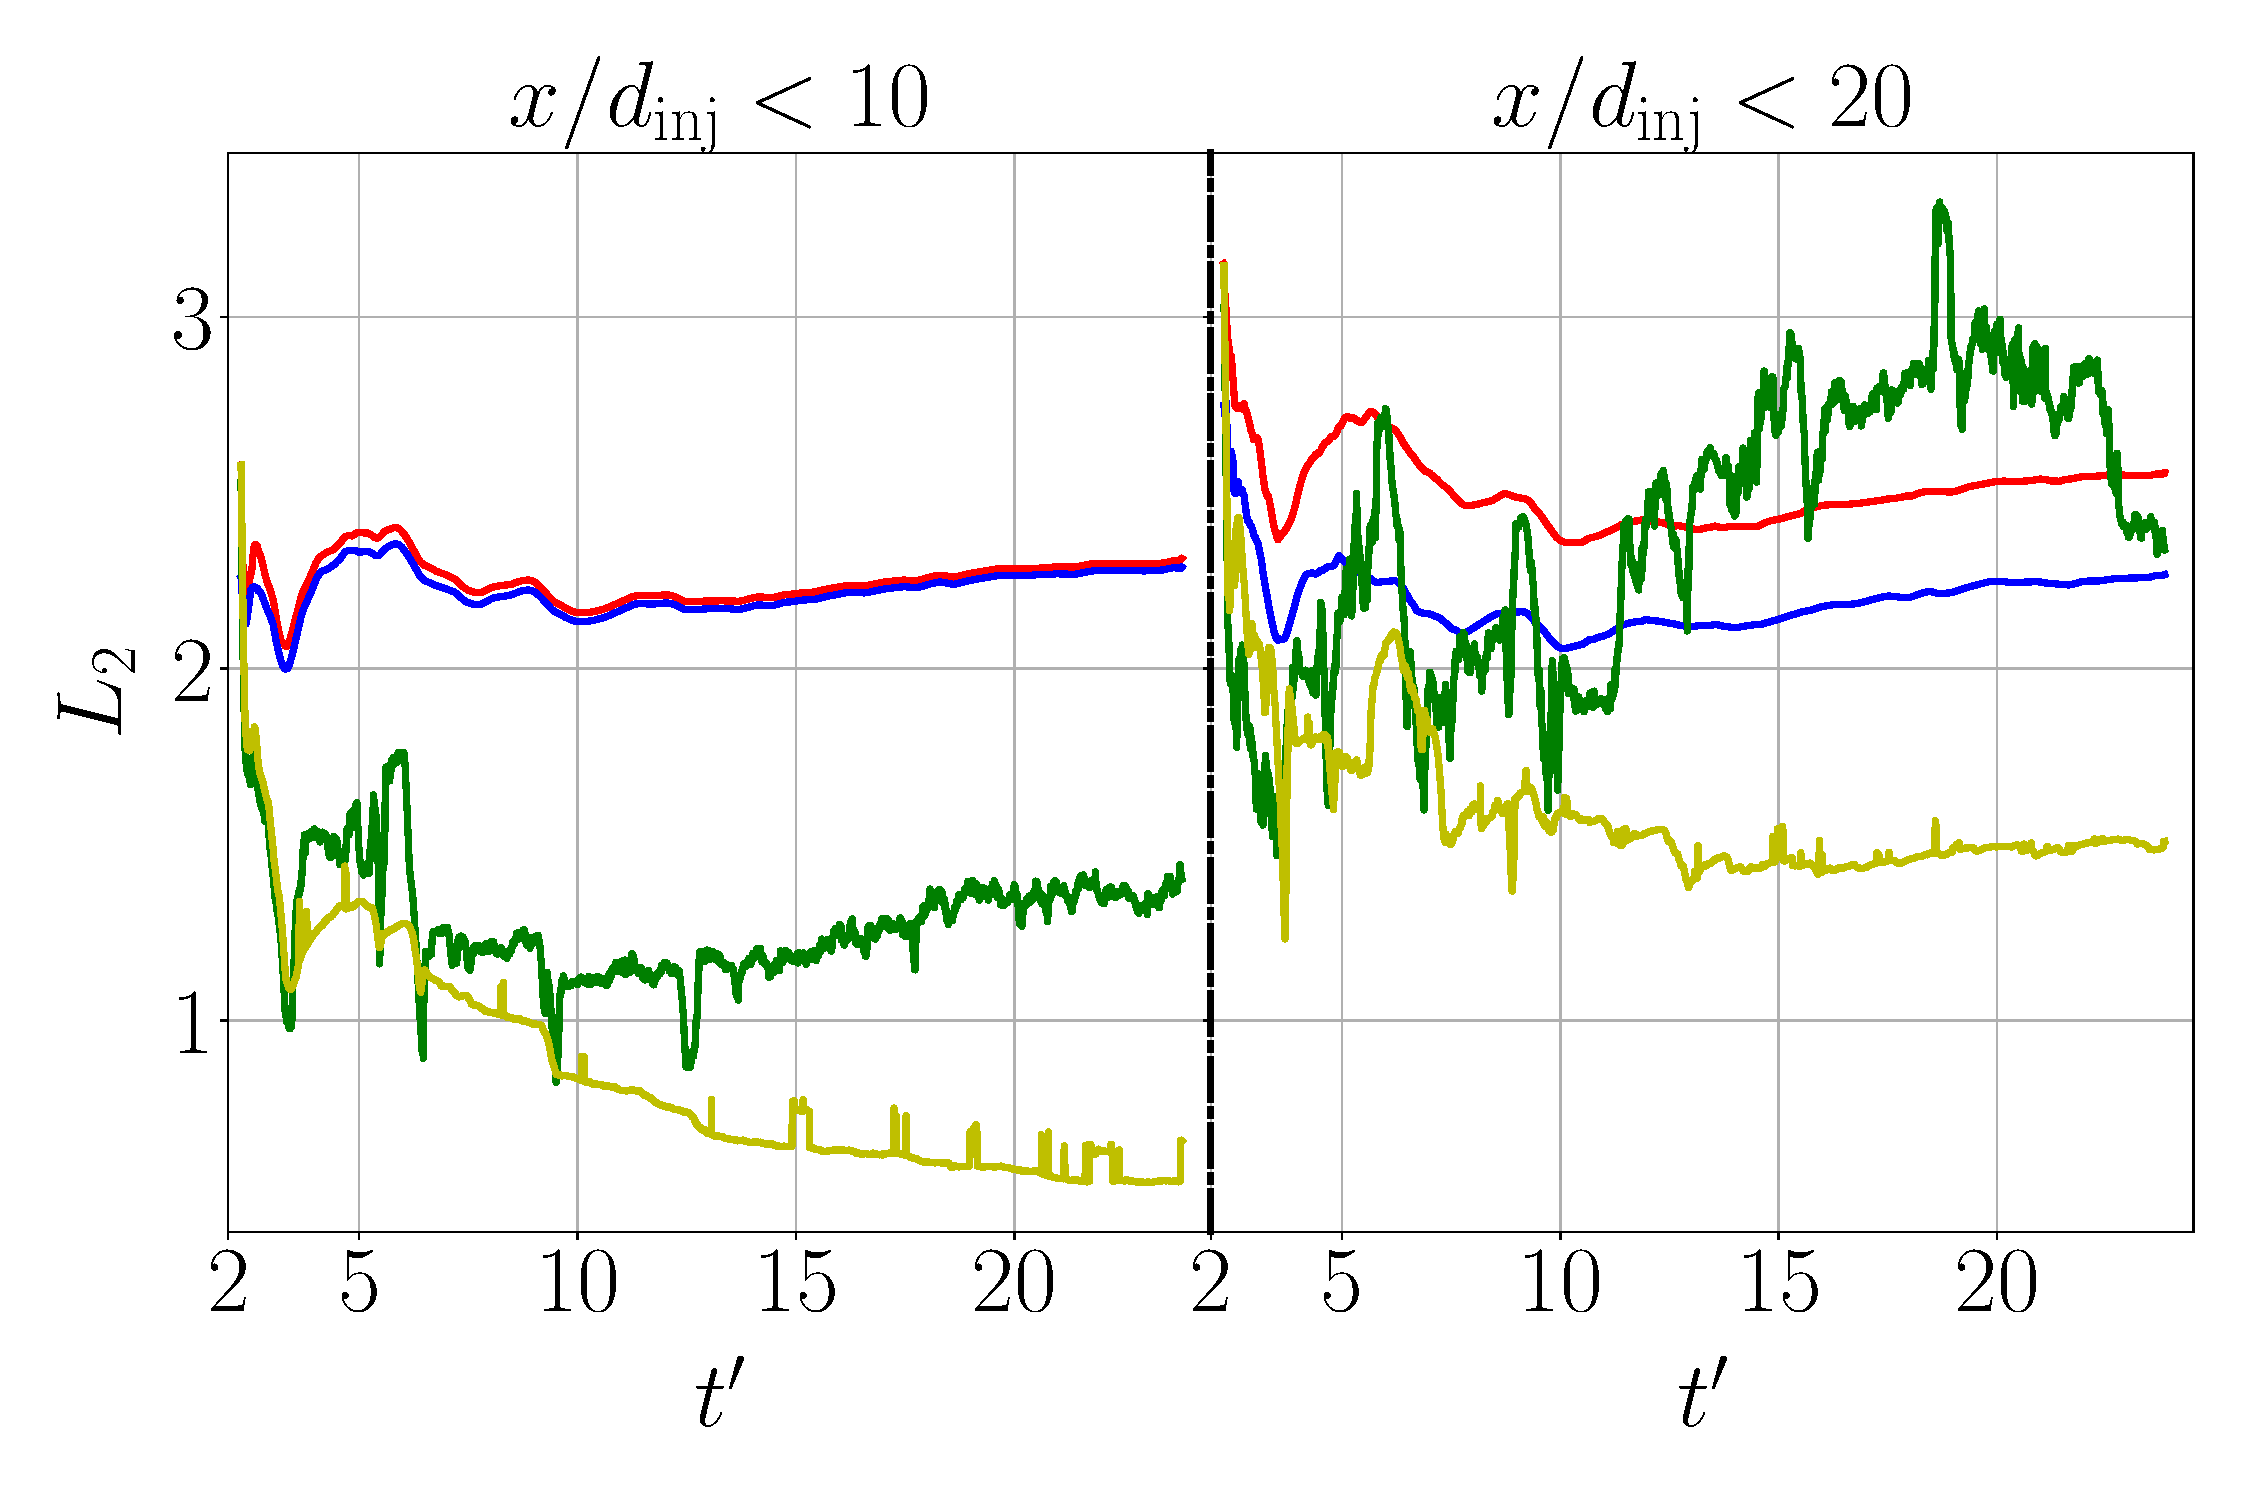
\includegraphics[scale=0.25]{./part2_developments/figures_ch5_resolved_JICF/results_trajectories/methods_comparison_L2_evolution_q6uG100_dx20_shared_y_axis.pdf}
   \vspace*{-0.25in}
   \caption{$L_2$ error evolution for two $x/d_\mathrm{inj}$ ranges}
   %\caption{$L_2$ error evolution }
   %\label{}
\end{subfigure}
\caption{Trajectories and $L_2$ errors obtained with different methods for case UG100\_DX20}
\label{fig:JICF_trajectories_and_L2_comparison}
\end{figure}

The evolution of the $L_2$ norm calculated with Eq. (\ref{eq:L2_JICF}) is shown in Figure \ref{fig:JICF_trajectories_and_L2_comparison}b for all methods. The norm is calculated for two ranges in the $x$ axis: $x/d_\mathrm{inj} < 10$ and $x/d_\mathrm{inj} < 20$. The former (reduced range) considers the trajectories closer to the injector before a full disperse spray is present, and all $L_2$ norms show convergence. The norms from the instantaneous trajectories show similar values since the trajectories for $x/d_\mathrm{inj} < 10$ are always close. The mean field trajectories show noisier signals, with the case MEAN\_CONT yielding the lowest errors. When considering the range $x/d_\mathrm{inj} < 20$, the signals show different behaviours. Regarding the instantaneous-averaged trajectories, both show the same tendencies as in the reduced range, but with larger norms due to the divergence of both curves in the dispersed phase region. The trajectory from method MEAN\_CONT shows also convergence in the norm, but with a larger value than for the reduced range. On the other hand, the signal from method MEAN\_GRAD does not show convergence with time when the dispersed spray region is included. The reason is that the field $\nabla_z | \overline{\psi} |$ shows a very unstable behaviour with time in the dispersed spray, as opposed to the field $\overline{\psi}$. It is not sure whether this method will yield a converged $L_2$ if the simulation were run longer. The results from Figure \ref{fig:JICF_trajectories_and_L2_comparison} show the strong influence that the choice of postprocessing method can have on the resulting trajectory.  \\

For validating experimentally the trajectories from the rest of the simulations, the method MEAN\_GRAD is selected due to its similarity with the methodology followed by \citeColor[becker_breakup_2002] to obtain the experimental correlation. Results are shown in Figure \ref{fig:JICF_trajectories_validation} for both operating points, including the case for the high $We$ number without synthetic turbulence injection. The evolution of the $L_2$ norm displayed has been obtained for the range $x/d_\mathrm{inj} < 10$. Additionally, an error along the trajectory  $\varepsilon_i$ is also defined to indicate the trajectory’s accuracy along the crossflow’s direction $x$:

\begin{equation}
\label{eq:error_along_trajectory}
\varepsilon_i  =  \frac{ z/d_\mathrm{inj} \Bigr|_{\mathrm{num},i} - z/d_\mathrm{inj} \Bigr|_{\mathrm{exp},i} }{ z/d_\mathrm{inj} \Bigr|_{\mathrm{exp},i} }
\end{equation}



Trajectories are shown in Figures \ref{fig:JICF_trajectories_validation}a and b for both operating points. The first remarkable events are the dependence on mesh resolution for both operating points, and the differentiation of two regions with axial distance along the trajectories. From the graphs, the regions can be distinguished as follows:

\begin{enumerate}

	\item A first near-injector region in which both resolutions coincide with the experimental correlation, showing no dependence on the mesh resolution. This regions extends up to $x/d_\mathrm{inj} \sim 5$ for low $We$ and to $x/d_\mathrm{inj} \sim 4$ for high $We$. Here, the dense core is located and primary atomization takes place, resulting in an accurate trajectory prediction.
	
	\item After the near-injector region, trajectories diverge and show different trends: the coarse simulation underestimates the experimental correlation, while the fine one continues within the confidence interval of the experiments until it surpasses it. This is the region where secondary atomization is forming droplets and a dispersed spray starts to be formed, hence mispredicting the experimental correlations.

\end{enumerate}

\clearpage



\begin{figure}[ht]
\flushleft
\begin{subfigure}[b]{0.45\textwidth}
	\centering
   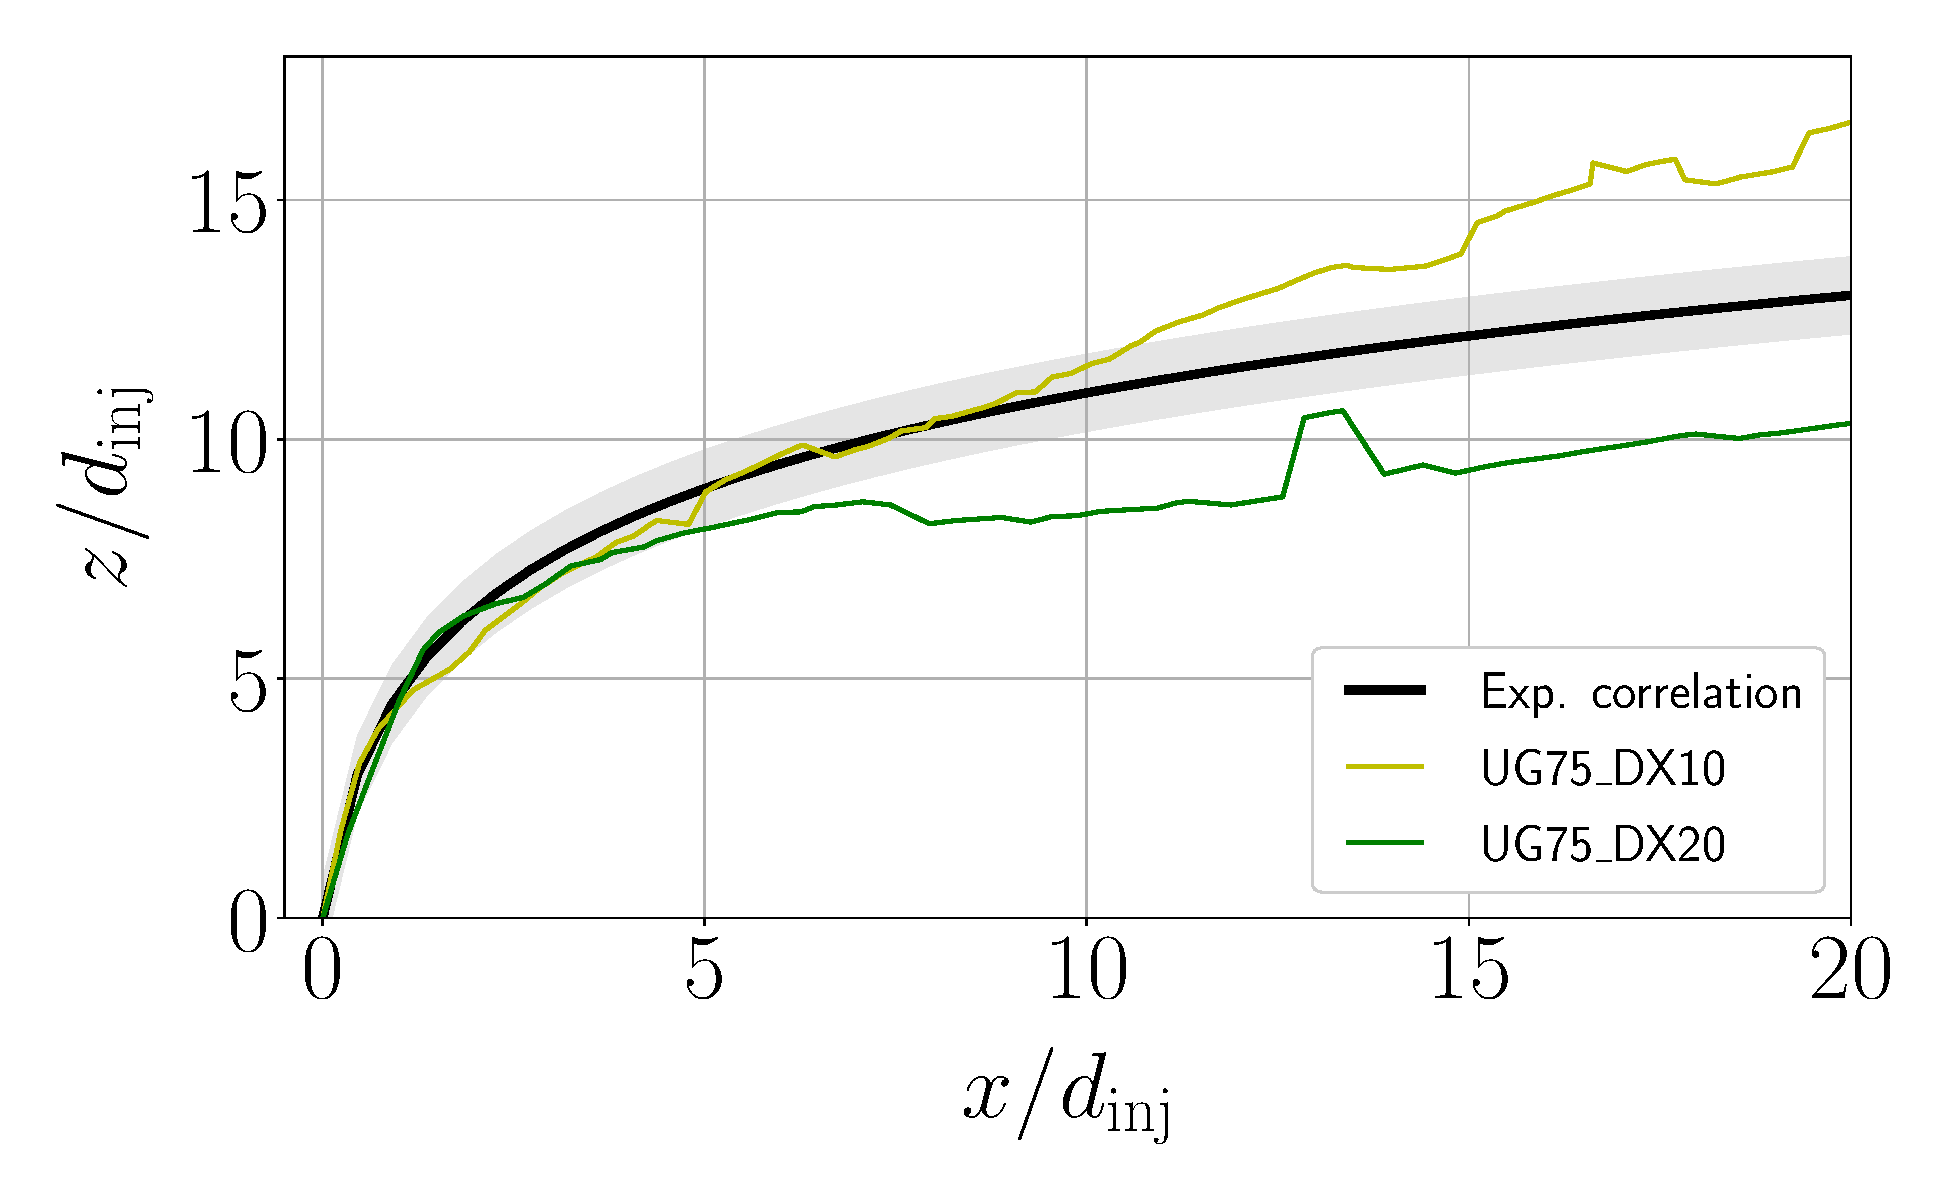
\includegraphics[scale=0.25]{./part2_developments/figures_ch5_resolved_JICF/results_trajectories/methods_expe_validation_trajectories_q6uG75.pdf}
   \vspace*{-0.25in}
   \caption{Low $We$ trajectories}
   %\label{} 
\end{subfigure}
%\hfill
\hspace{0.25in}
\begin{subfigure}[b]{0.45\textwidth}
	\centering
   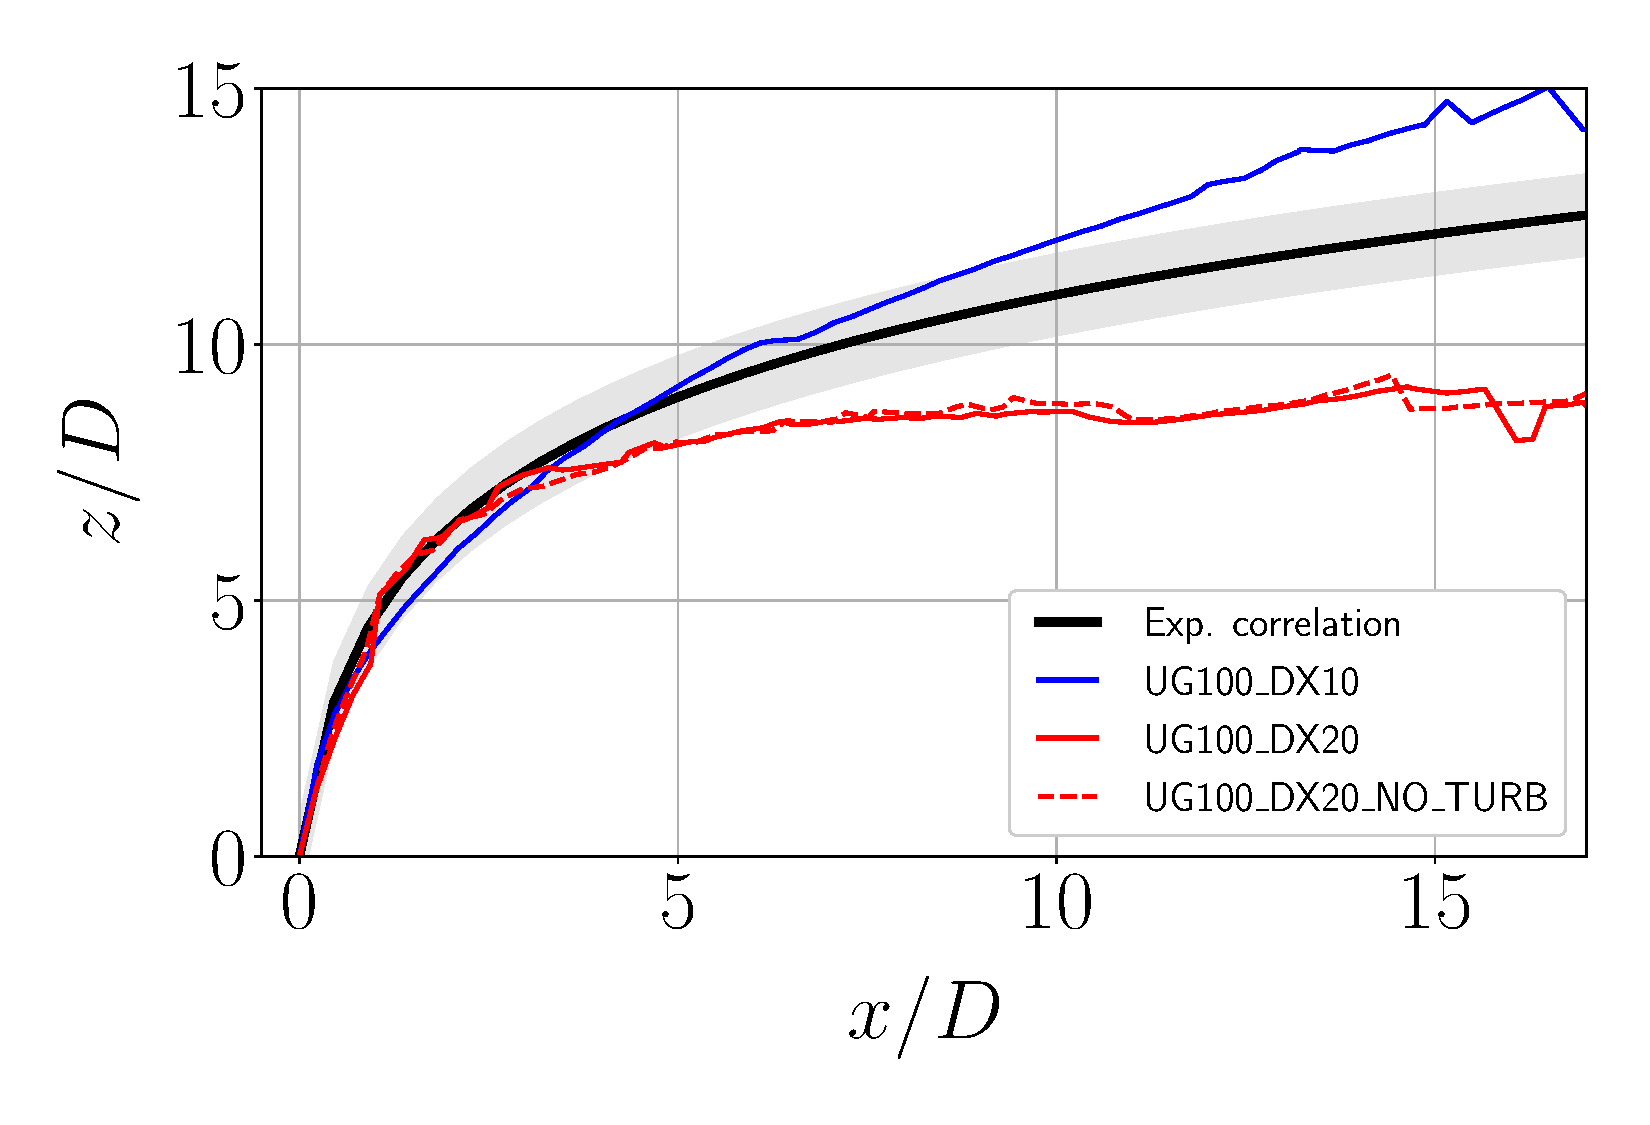
\includegraphics[scale=0.25]{./part2_developments/figures_ch5_resolved_JICF/results_trajectories/methods_expe_validation_trajectories_q6uG100.pdf}
   \vspace*{-0.30in}
   \caption{High $We$ trajectories}
   %\label{}
\end{subfigure}

\vskip\baselineskip
\vspace*{-0.2in}

\begin{subfigure}[b]{0.45\textwidth}
	\centering
   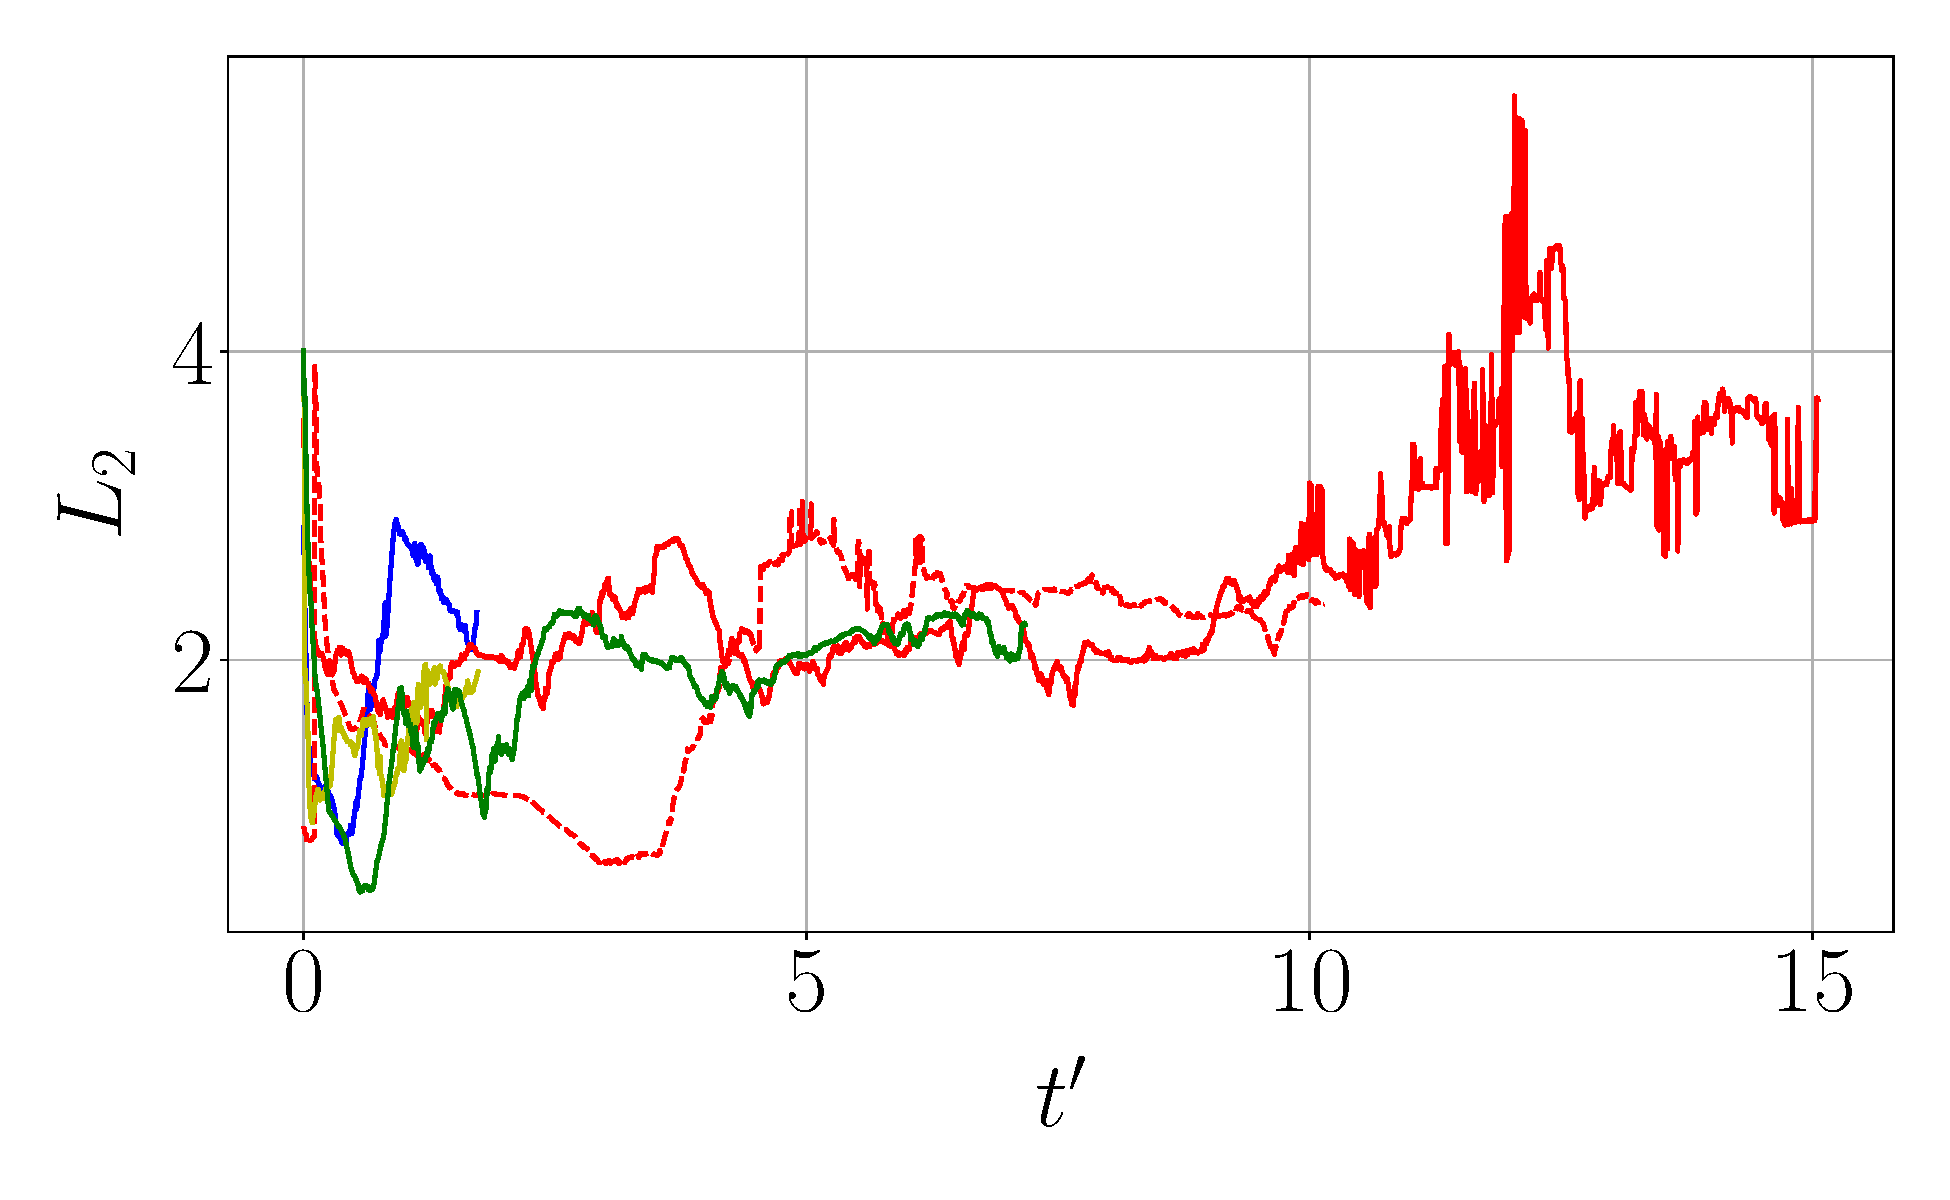
\includegraphics[scale=0.25]{./part2_developments/figures_ch5_resolved_JICF/results_trajectories/methods_expe_validation_L2_evolution.pdf}
   \vspace*{-0.25in}
   \caption{Evolution of $L_2$ norms with time.}
   %\label{} 
\end{subfigure}
%\hfill
\hspace{0.25in}
\begin{subfigure}[b]{0.45\textwidth}
	\centering
   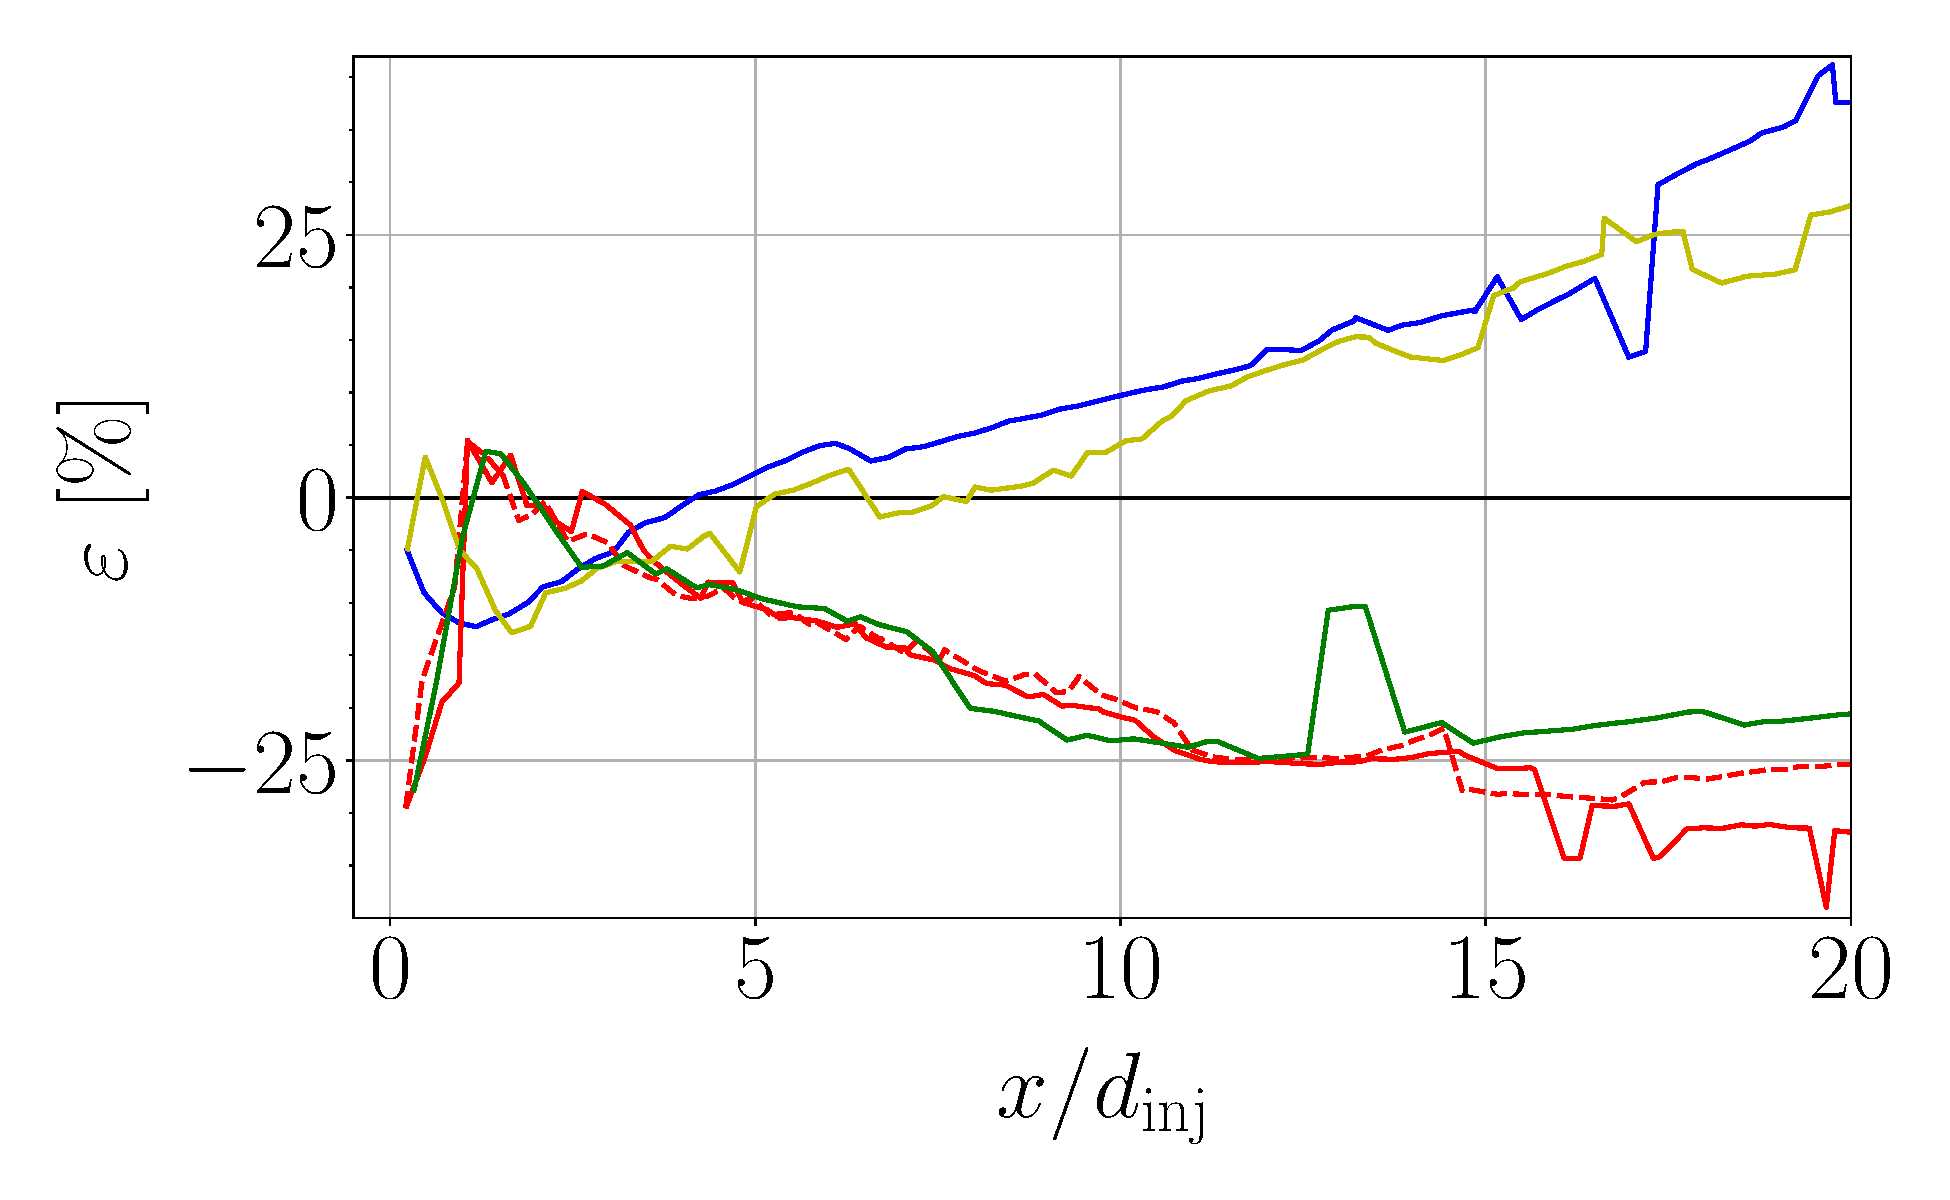
\includegraphics[scale=0.25]{./part2_developments/figures_ch5_resolved_JICF/results_trajectories/methods_expe_validation_error_with_xD.pdf}
   \vspace*{-0.30in}
   \caption{Error $\varepsilon$ along trajectory}
   %\label{}
\end{subfigure}


\caption{Trajectories and errors obtained with method MEAN\_GRAD}
\label{fig:JICF_trajectories_validation}
\end{figure}

\vspace*{-0.05in}

The reason why coarse simulations underestimate the trajectory further downstream, while the fine ones overestimate it, is the resolution of instabilities in the windward side of the jet (discussed previously in $\S$\ref{subsubsec:ch5_breakup_topology}).  Instabilities in the fine simulations create ligaments and droplets with high vertical velocities that penetrate further away than those generated in the coarse simulations. Consequently, their resulting trajectories penetrate further than the coarse ones and the experimental correlation after breakup occurs. 


Regarding the effect of injecting turbulence at the gaseous inlet, the red lines of Figure \ref{fig:JICF_trajectories_validation}b show that the mean trajectory is not affected when turbulence is added. The turbulence levels (as calculated in Appendix \ref{app:gas_initial_cond_JICF}) do not have an influence on the formation of instabilities for the case studied. Nevertheless, only the coarse resolution has been simulated without turbulence injection: further studies could include a simulation with a finer resolution in order to determine if the injected turbulence have an effect on the instabilities formed in the windward side of the column.

Figure \ref{fig:JICF_trajectories_validation}c shows the $L_2$ norm evolution. The coarse cases show convergence while the fine ones are still fluctuating, yet they seem to stabilize (simulations should run longer to confirm this). The final values for the errors are summarized in Table \ref{tab:jicf_L2_errors}, confirming that smaller deviations are obtained for fine resolutions. Finally, the relative error along the trajectory $\varepsilon$ is displayed in Figure \ref{fig:JICF_trajectories_validation}d. Negative values indicate underestimation of the experimental correlation, while positive ones indicate overestimation. In the vicinity of the injection nozzle ($x = 0$), errors are large because the denominator of Eq. (\ref{eq:error_along_trajectory}) is small. Then, deviations are small in the near injector region and start to increase monotonically in absolute value further downstream. Fine simulations present positive erros since they overestimate the experimental correlation, while the coarse ones yield negative ones due to the underestimation. This graph is useful to get an idea on the error commited in the vertical boundary of the spray when placing an SLI. For instance, if an injector is placed at $x = 5$ mm ($x/d_\mathrm{inj} \sim 11$), an SLI obtained from the fine resolution would yield low errors ($\sim 0~\%$ for UG75\_DX10 and $\sim 10~\%$ for UG100\_DX10), but very high ones for a coarse injector ($\sim - 25~\%$). %Placing an injector further downstream would increase the errors for any resolution. These effects will be studied in Chapter \ref{ch6:jicf_lgs_simulations}.



\begin{table}[!h]
\centering
\caption{$L_2$ errors for JICF simulations performed.}
\vspace*{-0.1in}
\begin{tabular}{cccccc}
\thickhline
\textbf{Case} &  UG75\_DX10 & UG75\_DX20 & UG100\_DX10 & UG100\_DX20 &  UG100\_DX20\_NT \\
\hline
$L_2$ & 0.29 & 1.16 & 0.44 & 1.40 & 1.35 \\
\thickhline
\end{tabular}
\label{tab:jicf_L2_errors}
\end{table}








\clearpage



\subsection{Turbulent structures in the gaseous field}
\label{ch5:subsec_turbulent_structures_in_gaseous_field}


Resolved simulations capture the liquid dense core, which perturbs the incoming air and creates turbulence downstream the injector. This perturbation effect is illustrated in Figure \ref{fig:jet_air_interaction_up_and_skeleton}. At the left, the instantaneous axial velocity fluctuations $u'$ and the jet interface in the middle plane y = 0 are plotted. The dense core creates turbulence downstream the injection point, as shown by the strong fluctuations. Such perturbations can have a great impact on secondary atomization and spray dispersion once primary breakup has taken place. Therefore, modeling this perturbance effect as accurate as possible is paramount for later performing dispersed-phase simulations (Chapter \ref{ch6:jicf_lgs_simulations}), where the dense core is a priori neglected and a developed spray is injected. A three-dimensional view of the perturbation effect is depicted in Figure \ref{fig:jet_air_interaction_up_and_skeleton} right, where the gaseous streamlines are visualized. Two main turbulent structures appear: a horseshoe vortex formed at the wall right upstream the liquid jet, widely observed in literature dealing with both gaseous and liquid JICF \citemColor[fric_vortical_1994,karagozian_transverse_2010,schlegel_contributions_2011], and a recirculation zone right downstream the jet. The latter, which is a is characteristic of JICF configurations at high gaseous velocities \citepColor[fontes_improved_2019], might entrap droplets emanating from the ligaments formed during column breakup and affect their trajectory and subsequent secondary breakup. 

\begin{figure}[ht]
\flushleft
\includeinkscape[inkscapelatex=false,scale=1.1]{./part2_developments/figures_ch5_resolved_JICF/turbulent_structures/jet_air_interaction_up_and_streamlines_vortices}
\caption[Interaction between liquid dense core and gaseous phase.]{Interaction between liquid dense core and gaseous phase. \textsl{Left}: Instantaneous $u'$ field in a JICF simulation from case UG100\_DX20. The black contours indicate the lines with zero instantaneous fluctuation $u' = 0$, while the white contours denote the location of the interface at the plane. \textsl{Right}: 3D streamlines in case UG100\_DX20}
\label{fig:jet_air_interaction_up_and_skeleton}
\end{figure}


In this section, the turbulent structures created as a consequence of the dense core presence are studied. These results will be used in Chapter \ref{ch6:jicf_lgs_simulations} to compare with the disturbance effects in the gaseous field modeled in the dispersed phase simulations. The gaseous field is investigated by analyzing the mean axial gaseous velocity field $\overline{u}$ in the planes illustrated in Figure \ref{fig:jicf_sps_with_gaseous_planes}. %These planes are: the symmetry plane $y = 0$ mm, planes perpendicular to the crossflow $x = 5, 10$ mm (which correspond to the planes where spray has been sampled and postprocessed, see Figure \ref{fig:jicf_interior_boundaries_surface_measurements}), and the planes perpendicular to the injection directions $z = 0.2, 0.8, 1.6$ mm. 


\begin{figure}[h!]
	\centering
	\includeinkscape[inkscapelatex=false,scale=0.8]{./part2_developments/figures_ch5_resolved_JICF/turbulent_structures/jicf_sps_with_gaseous_planes}
	\caption{Jet from case UG100\_DX10 showing planes to study the gaseous phase}
	% NOTA: figura de pilotage 2021_05_21
	% OJO: mirar pilotages  reunion_Thierry_2021_01_22, 2021_02_04, 2021_05_21, 2021_05_25 
	\label{fig:jicf_sps_with_gaseous_planes}
\end{figure}


Mean axial velocity at the symmetry plane $y = 0$ mm for all cases are shown in Figure \ref{fig:JICF_turbulent_structures_plane_y0} (case UG100\_DX20\_NT  is not displayed in this section since its mean fields are identical to those of case UG100\_DX20). The region with mean liquid obtained as $\overline{\psi} > 0.5$ is denoted in grey, hence the displayed velocities correspond only to the mean gaseous region. Streamlines are also shown to indicate the flow direction. In all cases, a recirculation bubble enclosed by the white solid line is retrieved immediately downstream the dense core. This recirculation region is fully converged for the coarse cases but not for the fine ones. The effect of this bubble is to push the streamlines below and behind it upwards, hence confering the gas a positive vertical velocity downstream the dense core. Upstream the jet, the streamlines are initially oriented towards the axial direction but then bend vertically due to the presence of the dense core. These streamlines are again directed vertically due to the action of the recirculation bubble. In general, velocities are larger for the high Weber operating point except in the recirculation bubble, where mean negative axial velocities show the same values for both conditions.

\begin{figure}[ht]
\centering
   \includeinkscape[inkscapelatex=false,scale=0.2]{./part2_developments/figures_ch5_resolved_JICF/turbulent_structures/planes_y_ux_mean}

\caption[Mean axial velocity at plane $y = 0$ mm]{Mean axial velocity at plane $y = 0$ mm. Black lines with arrows are in-plane mean streamlines; the white solid line indicates the contour $\overline{u} = 0$ which delimites the recirculation bubble. The grey area  indicates the mean liquid region, identifed as $\overline{\psi} > 0.5$}
\label{fig:JICF_turbulent_structures_plane_y0}
\end{figure}

The $\overline{u}$ profiles along the dashed lines from Figure \ref{fig:JICF_turbulent_structures_plane_y0} are represented in Figures \ref{fig:JICF_sps_lines_y0_along_x_ux_mean} and  \ref{fig:JICF_sps_lines_y0_along_z_ux_mean}. Both graphs reveal that perturbations are stronger closer to the bottom wall (line $z = 1.6$ mm in Figure \ref{fig:JICF_sps_lines_y0_along_x_ux_mean}  traverses indeed the recirculation bubble, since velocities reach negative values). Figure \ref{fig:JICF_sps_lines_y0_along_x_ux_mean} shows that velocity profiles stabilize several diameters downstream the injection point to lower values than in the corresponding single-phase simulation (no jet, i.e. dotted line in the figures), which is due to momentum exchanged with the liquid. This gas energy transferred to the liquid has been invested in bending and atomizing the jet. Lines from Figure \ref{fig:JICF_sps_lines_y0_along_z_ux_mean} reflect that the recirculation bubble extends up to a location $x = 2.5$ mm, and that this one is actually insensitive to the operating point. This might suggest that the recirculation bubble is not affected by the Weber number and depends only on the $q$ factor, which is identical in both conditions. There is, however, a strong dependent on the interface resolution: profiles crossing the recirculation bubble are not greatly affected by resolution in the regions with the lowest velocities, while the opposite happens outside it, in the deceleration regions. Nevertheless, it is not sure whether the fields from the fine resolutions are fully converged, and hence the profiles depicted might still change if the simulations run for longer time.



\begin{figure}[ht]
\flushleft
\begin{subfigure}[b]{0.45\textwidth}
	\centering
   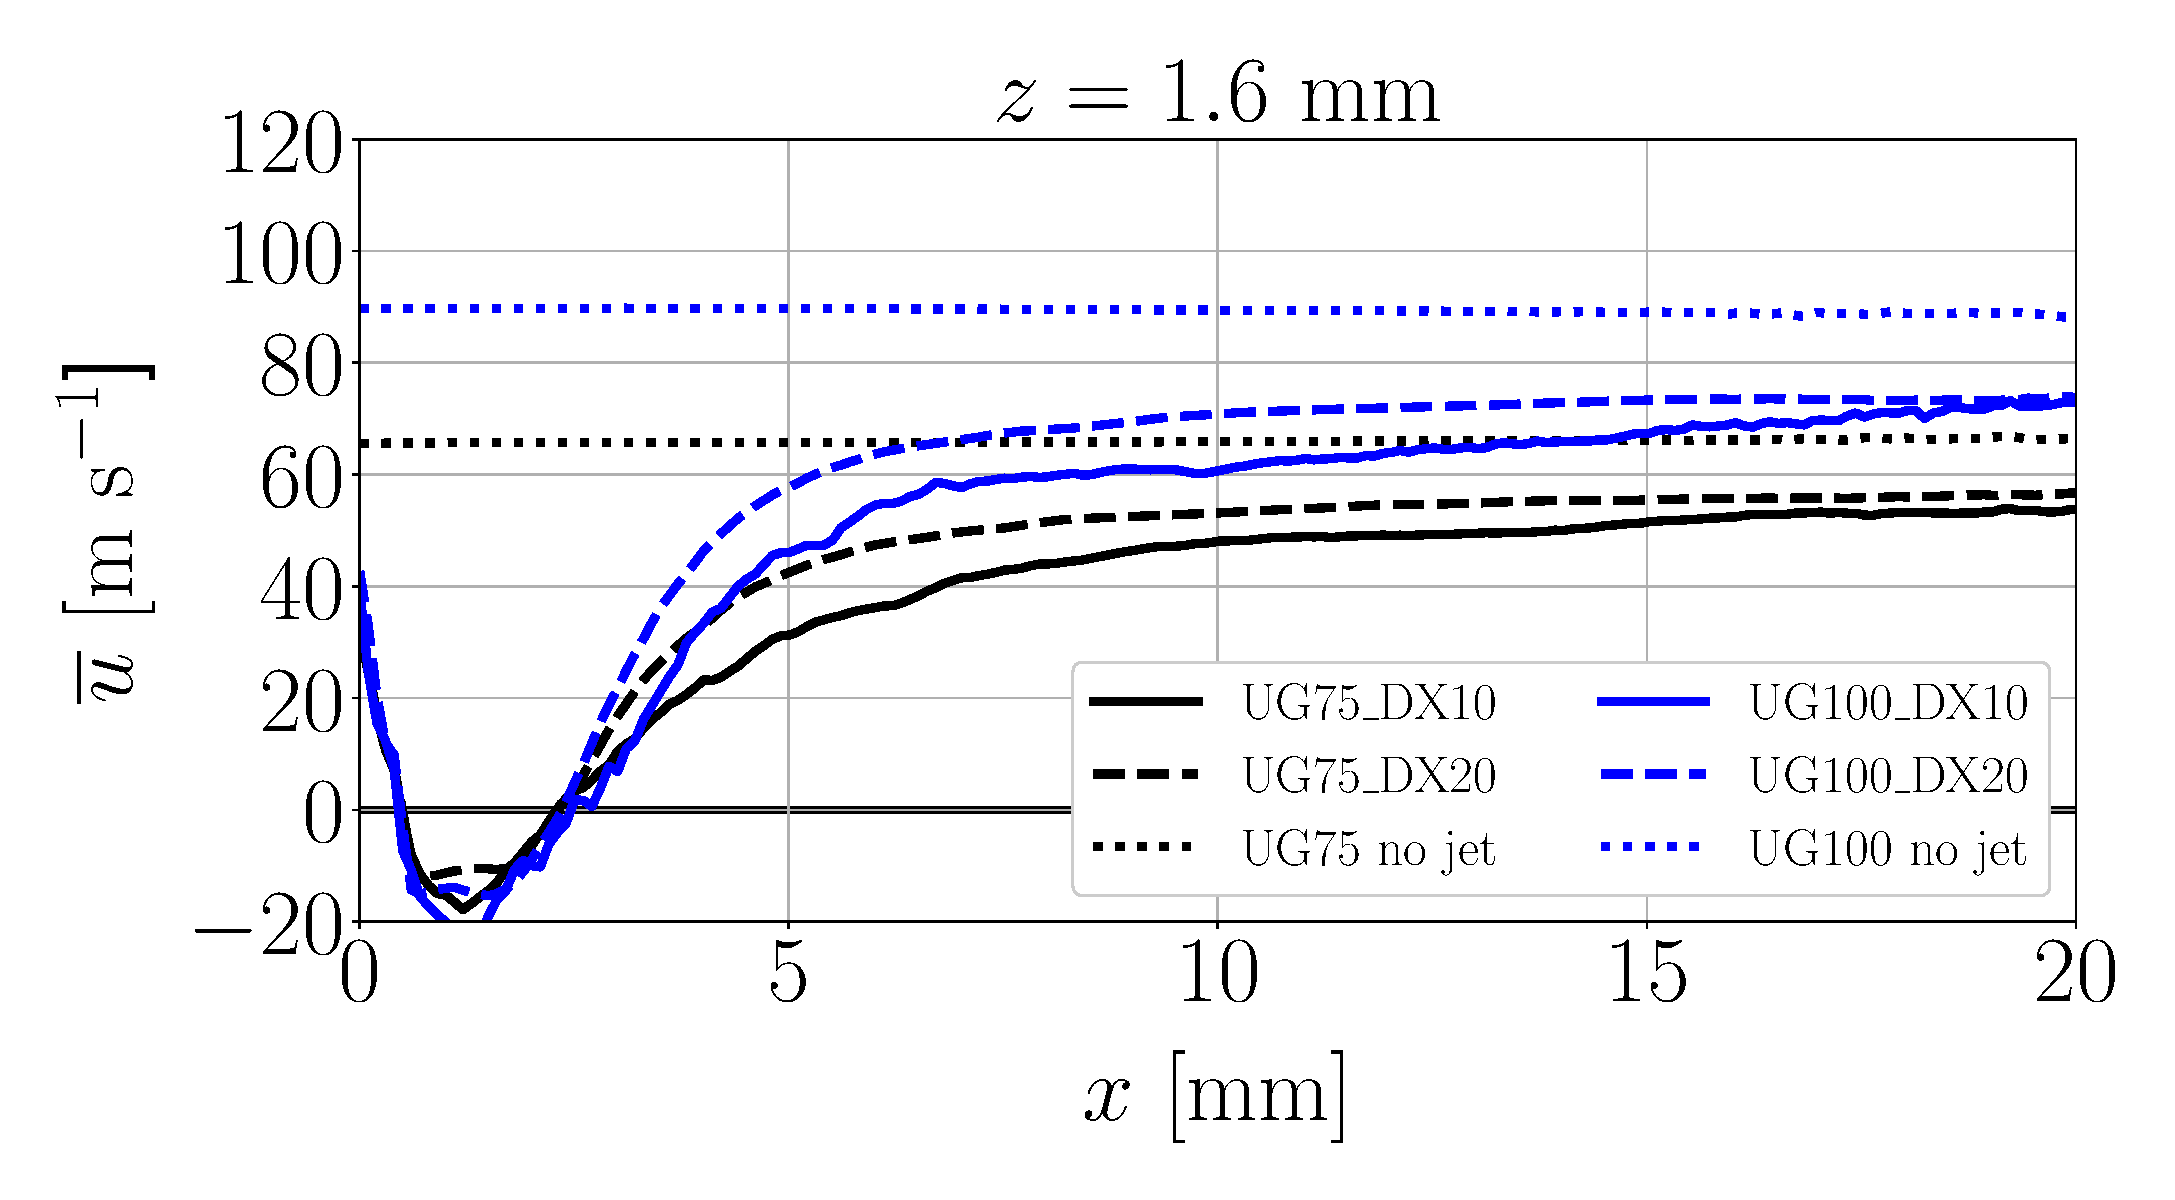
\includegraphics[scale=0.22]{./part2_developments/figures_ch5_resolved_JICF/turbulent_structures/line_y0_along_x_z01p6}
   %\caption{}
   %\label{} 
\end{subfigure}
\hspace{0.4in}
\begin{subfigure}[b]{0.45\textwidth}
	\centering
   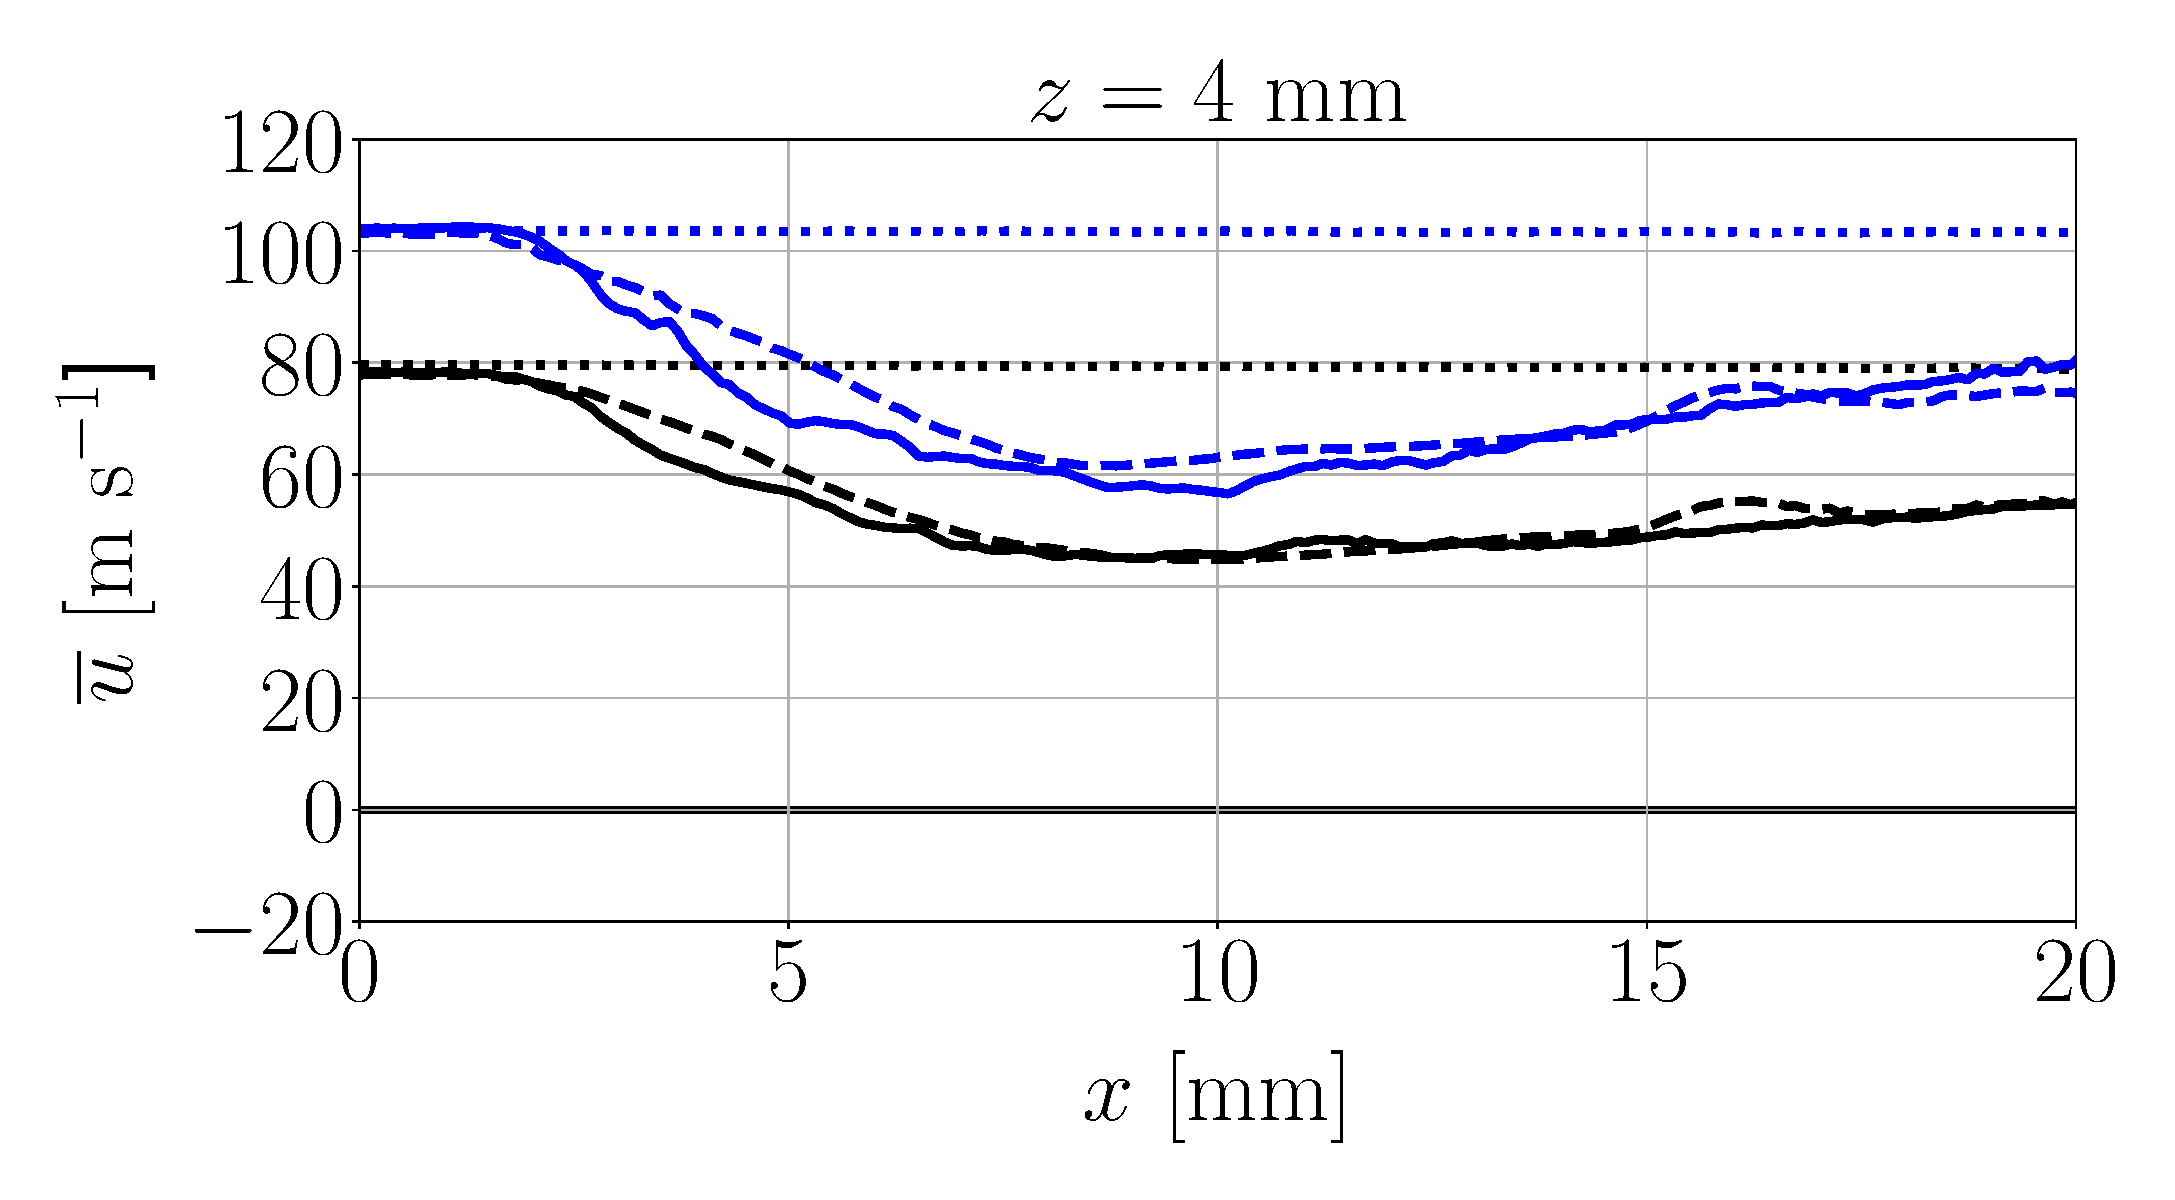
\includegraphics[scale=0.22]{./part2_developments/figures_ch5_resolved_JICF/turbulent_structures/line_y0_along_x_z04}
   %\caption{}
   %\label{}
\end{subfigure}
\caption{Mean axial velocity evolution along axial coordinate at locations $z = 1.6, 4$ mm in plane $y = 0$ (lines of Figure \ref{fig:JICF_turbulent_structures_plane_y0})}
\label{fig:JICF_sps_lines_y0_along_x_ux_mean}
\end{figure}


\clearpage


\begin{figure}[ht]
\flushleft
   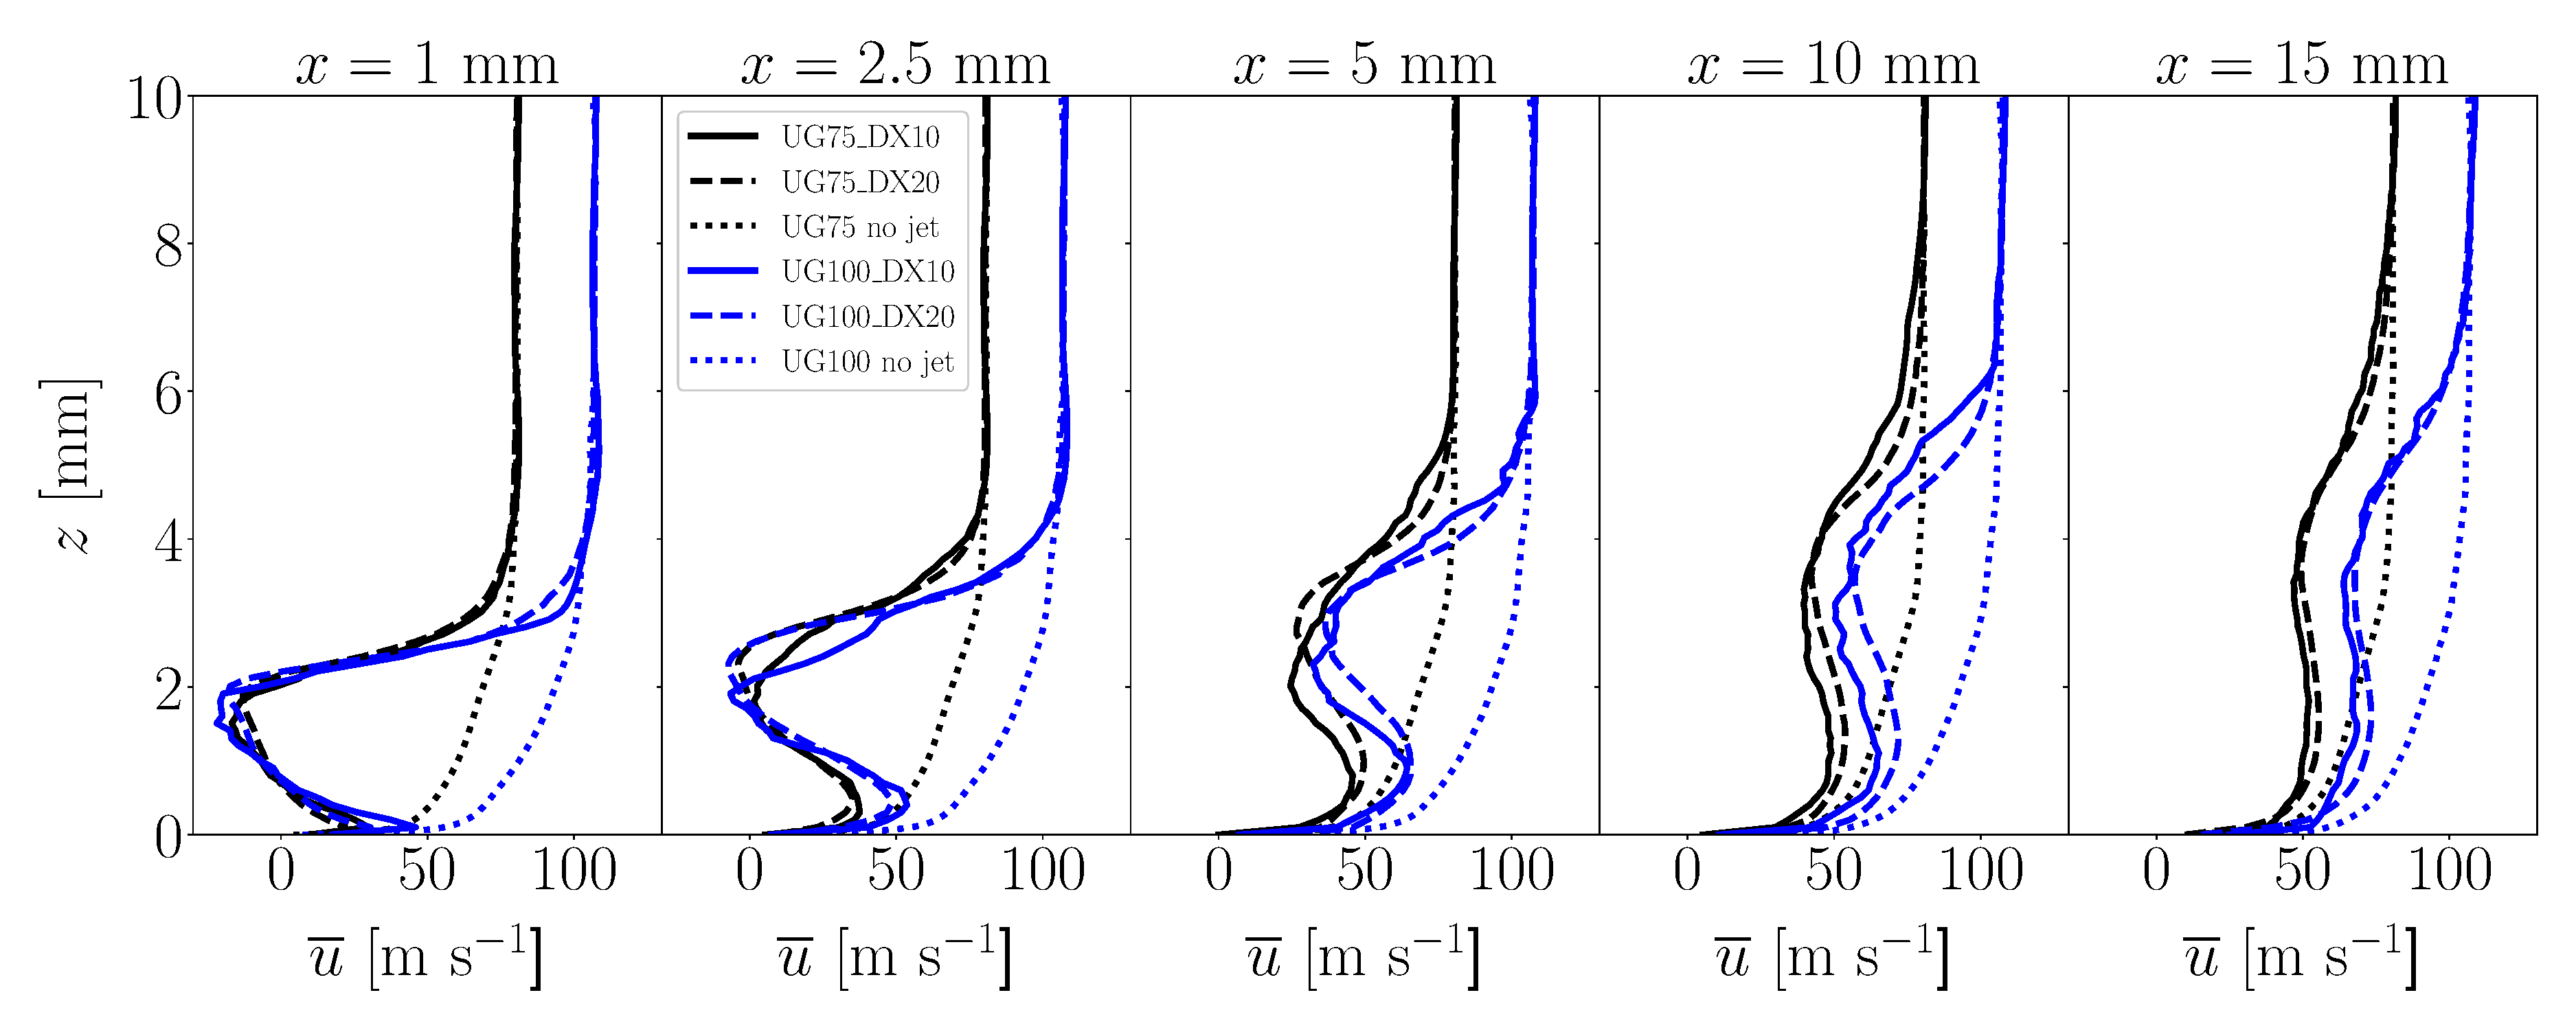
\includegraphics[scale=0.24]{./part2_developments/figures_ch5_resolved_JICF/turbulent_structures/lines_y0_along_z_ux_mean}
\caption{Mean axial velocity evolution along vertical coordinate at $x = 1, 2.5, 5, 10, 15$ mm locations of plane $y = 0$ (lines of Figure \ref{fig:JICF_turbulent_structures_plane_y0})}
\label{fig:JICF_sps_lines_y0_along_z_ux_mean}
\end{figure}


The mean fields at the liquid sampling planes $x = 5, 10$ mm are shown in Figure \ref{fig:JICF_turbulent_structures_planes_x}.  The perturbation effect of the dense core is observed by the deceleration around the central plane $y = 0$. Lower velocities are found at $x = 5$ mm than at 10 mm, since the perturbance effects are stronger further upstream as previously shown in Figure \ref{fig:JICF_sps_lines_y0_along_z_ux_mean}. All cases also retrieve vortical structures symmetrical with respect to the $y = 0$ axis, which rotate in counter-clockwise direction for $y > 0$ and in clockwise direction for  $y < 0$. These vortical structures in the gaseous phase, known as counter-rotating vortex pair (CVP), are a typical characteristic of the JICF and are found up to several diameter locations downstream the injection nozzle, having a strong effect on droplets dispersion \citepColor[arienti_aerodynamic_2006]. Figure \ref{fig:JICF_sps_lines_iso-x_along_y_ux_mean} shows the mean velocity profiles along the dashed lines from Figure \ref{fig:JICF_turbulent_structures_planes_x}. All profiles are symmetrical with respect to plane $y = 0$. Decelerations are stronger the closer to the wall ($z = 1.6$ mm) and the closer to the injection nozzle ($x = 5$ mm). All profiles show a dependence on the interface resolution, where larger differences are located at the regions with stronger decelerations. %The largest deviations are found at the  location $z = 5$ mm in the plane $x = 10$ mm, where the fine resolution shows lower velocities than the coarse one. This is attributed to disturbances created by the large ligaments shed from the liquid dense core (column breakup phenomenon), since these ones penetrate in the fine cases than in the coarse ones (see, for instance, Figure \ref{fig:jicf_column_breakup_ug100}).

\begin{figure}[ht]
\centering
   \includeinkscape[inkscapelatex=false,scale=0.24]{./part2_developments/figures_ch5_resolved_JICF/turbulent_structures/planes_x_ux_mean}
\caption[Mean axial velocity at planes $x = 5, 10$ mm]{Mean axial velocity at planes $x = 5, 10$ mm. Black lines with arrows are in-plane mean streamlines. Fields are symmetric around the $y = 0$, hence each picture shows the mean fields for equivalent operating condition and plane location but different resolution to ease visual comparison}
\label{fig:JICF_turbulent_structures_planes_x}
\end{figure}

\clearpage


\begin{figure}[ht]
\centering
\begin{subfigure}[b]{1.0\textwidth}
	\centering
   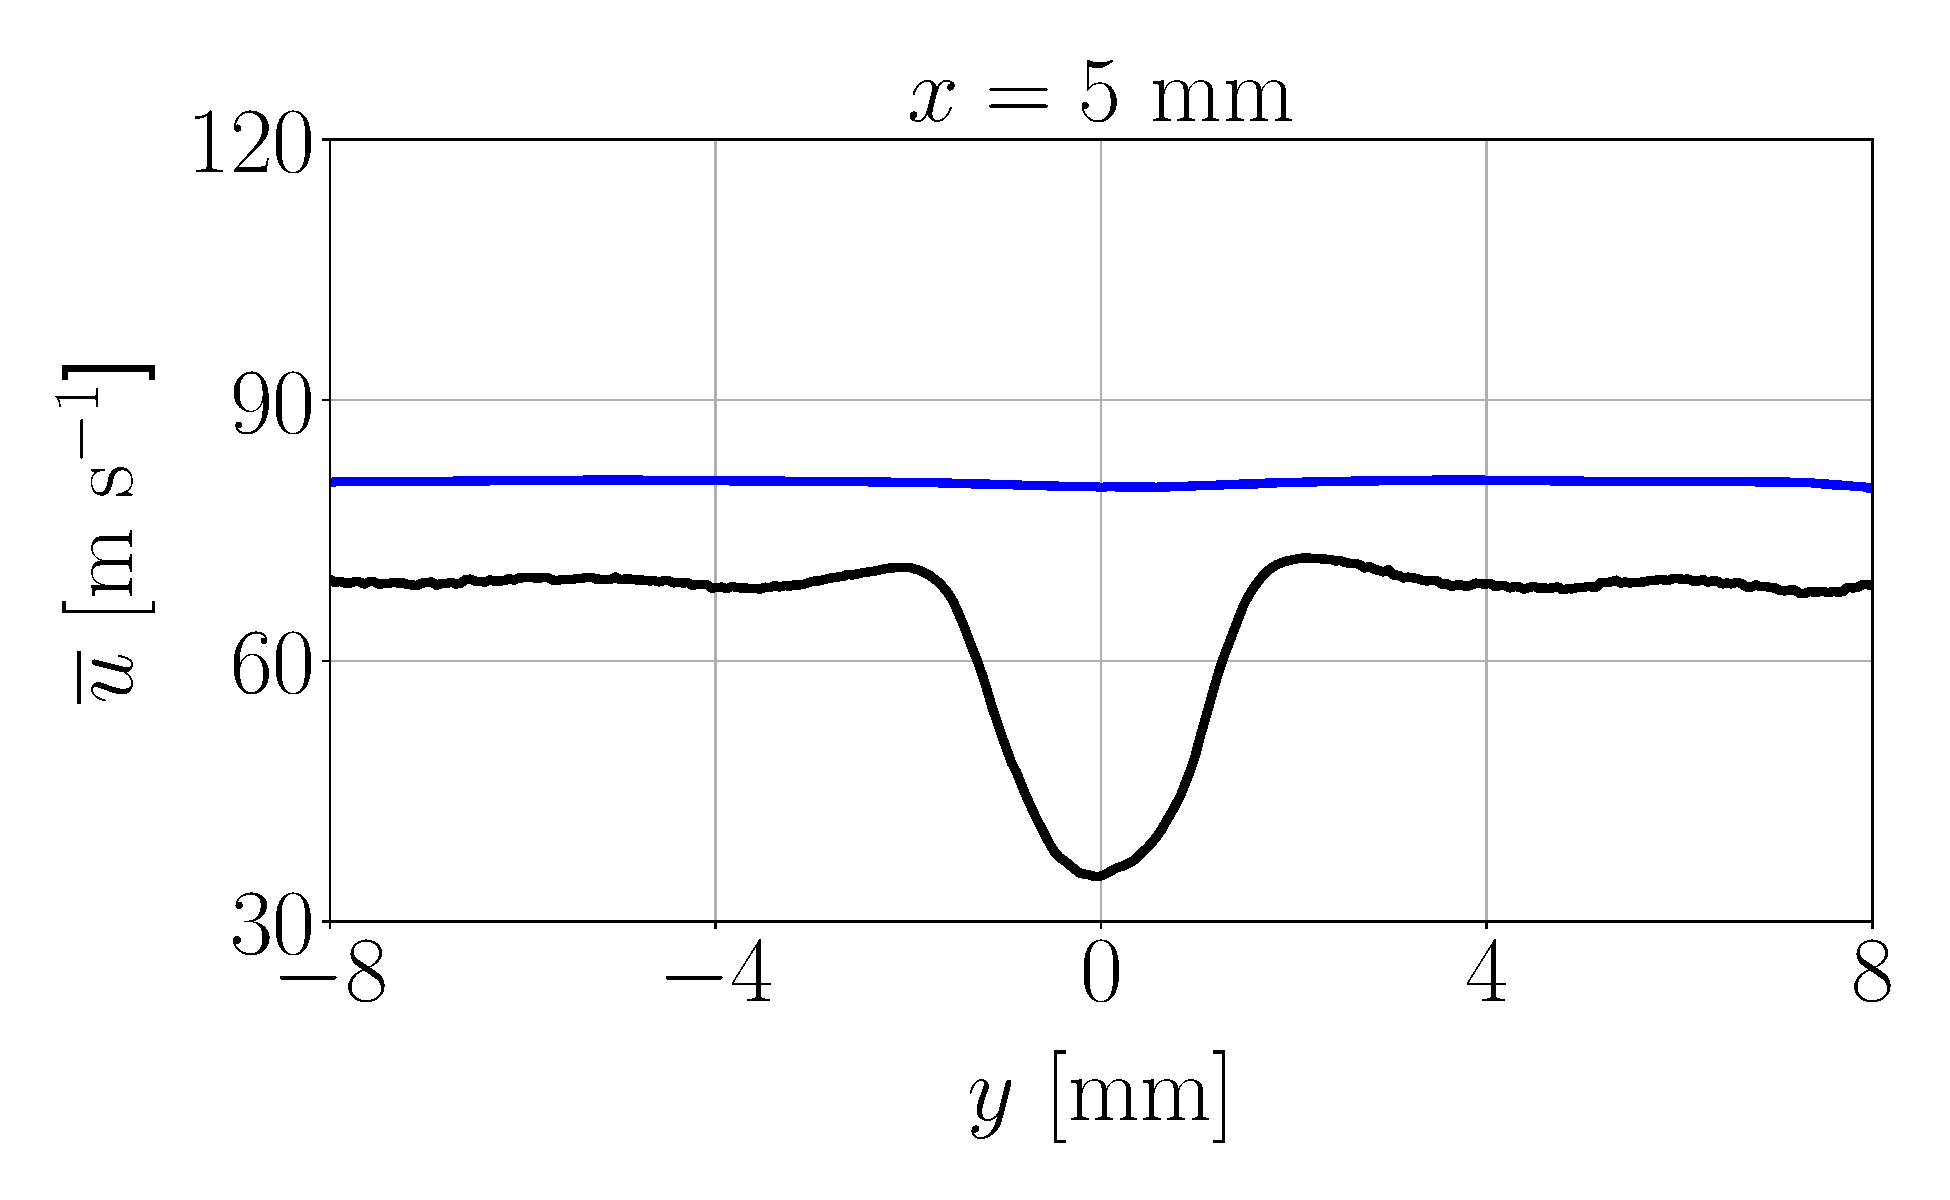
\includegraphics[scale=0.24]{./part2_developments/figures_ch5_resolved_JICF/turbulent_structures/lines_iso-x_along_y_ux_mean_UG75_x05}
   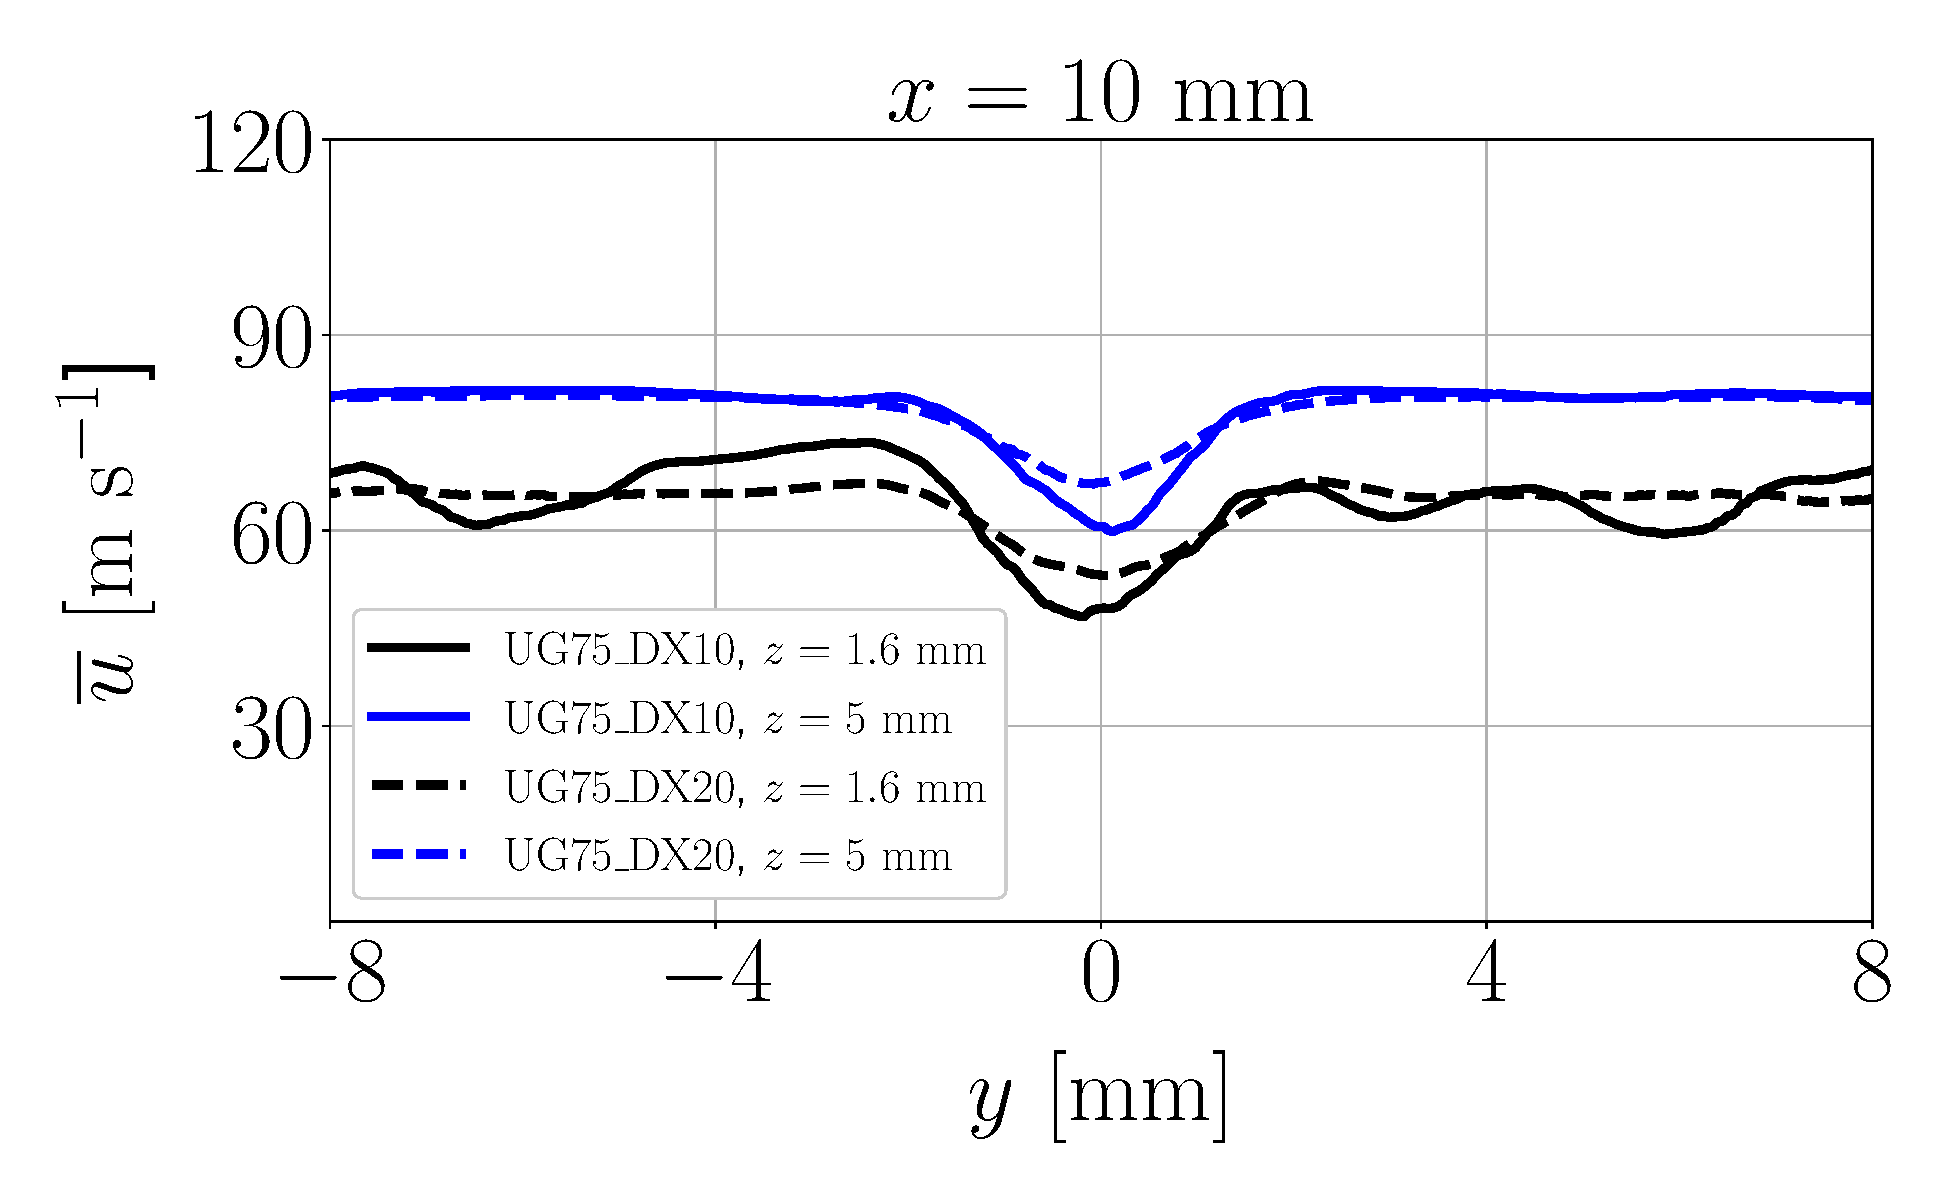
\includegraphics[scale=0.24]{./part2_developments/figures_ch5_resolved_JICF/turbulent_structures/lines_iso-x_along_y_ux_mean_UG75_x10}
   \vspace*{-0.1in}
	\caption{Low Weber operating point}
\end{subfigure}
\vskip\baselineskip
\begin{subfigure}[b]{1.0\textwidth}
	\centering
   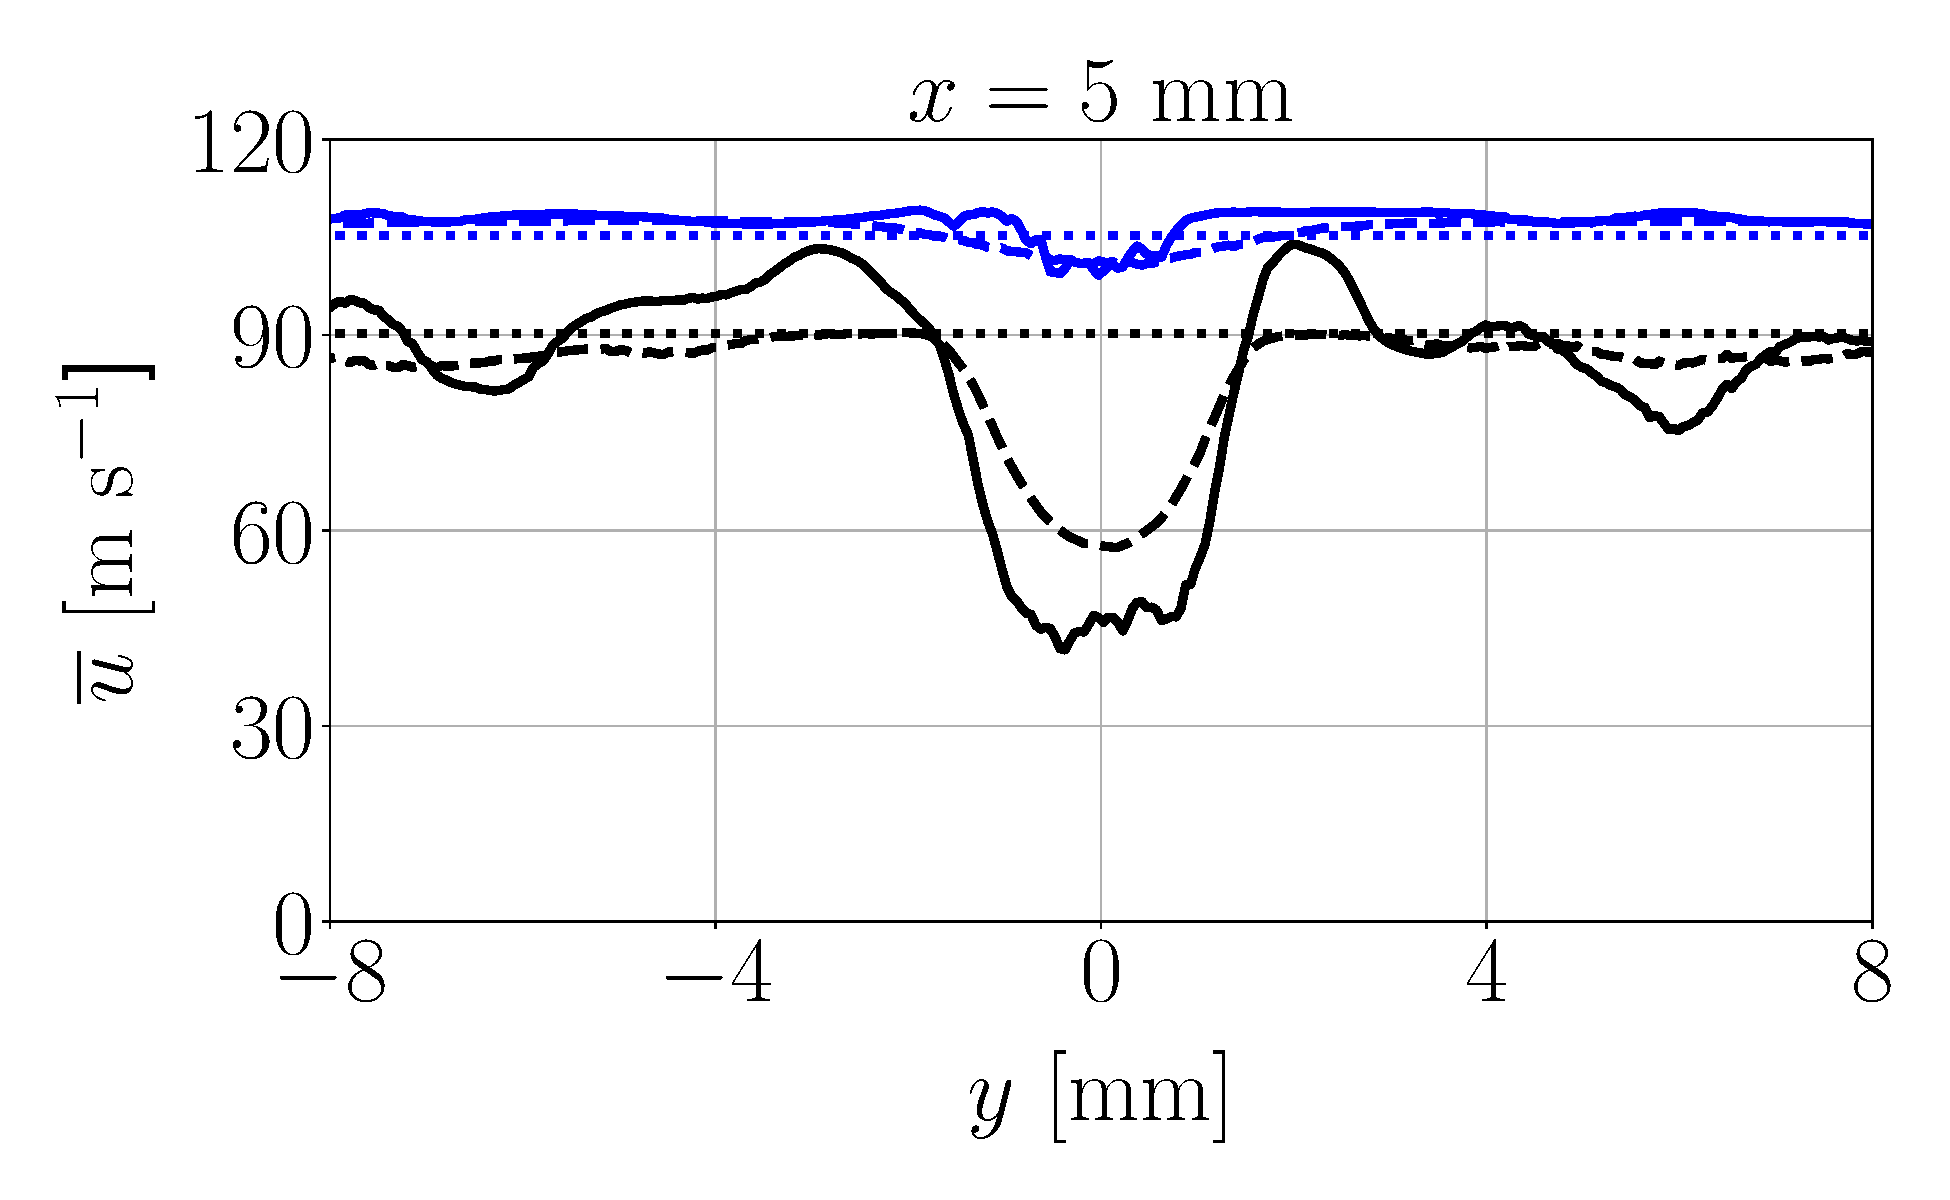
\includegraphics[scale=0.24]{./part2_developments/figures_ch5_resolved_JICF/turbulent_structures/lines_iso-x_along_y_ux_mean_UG100_x05}
   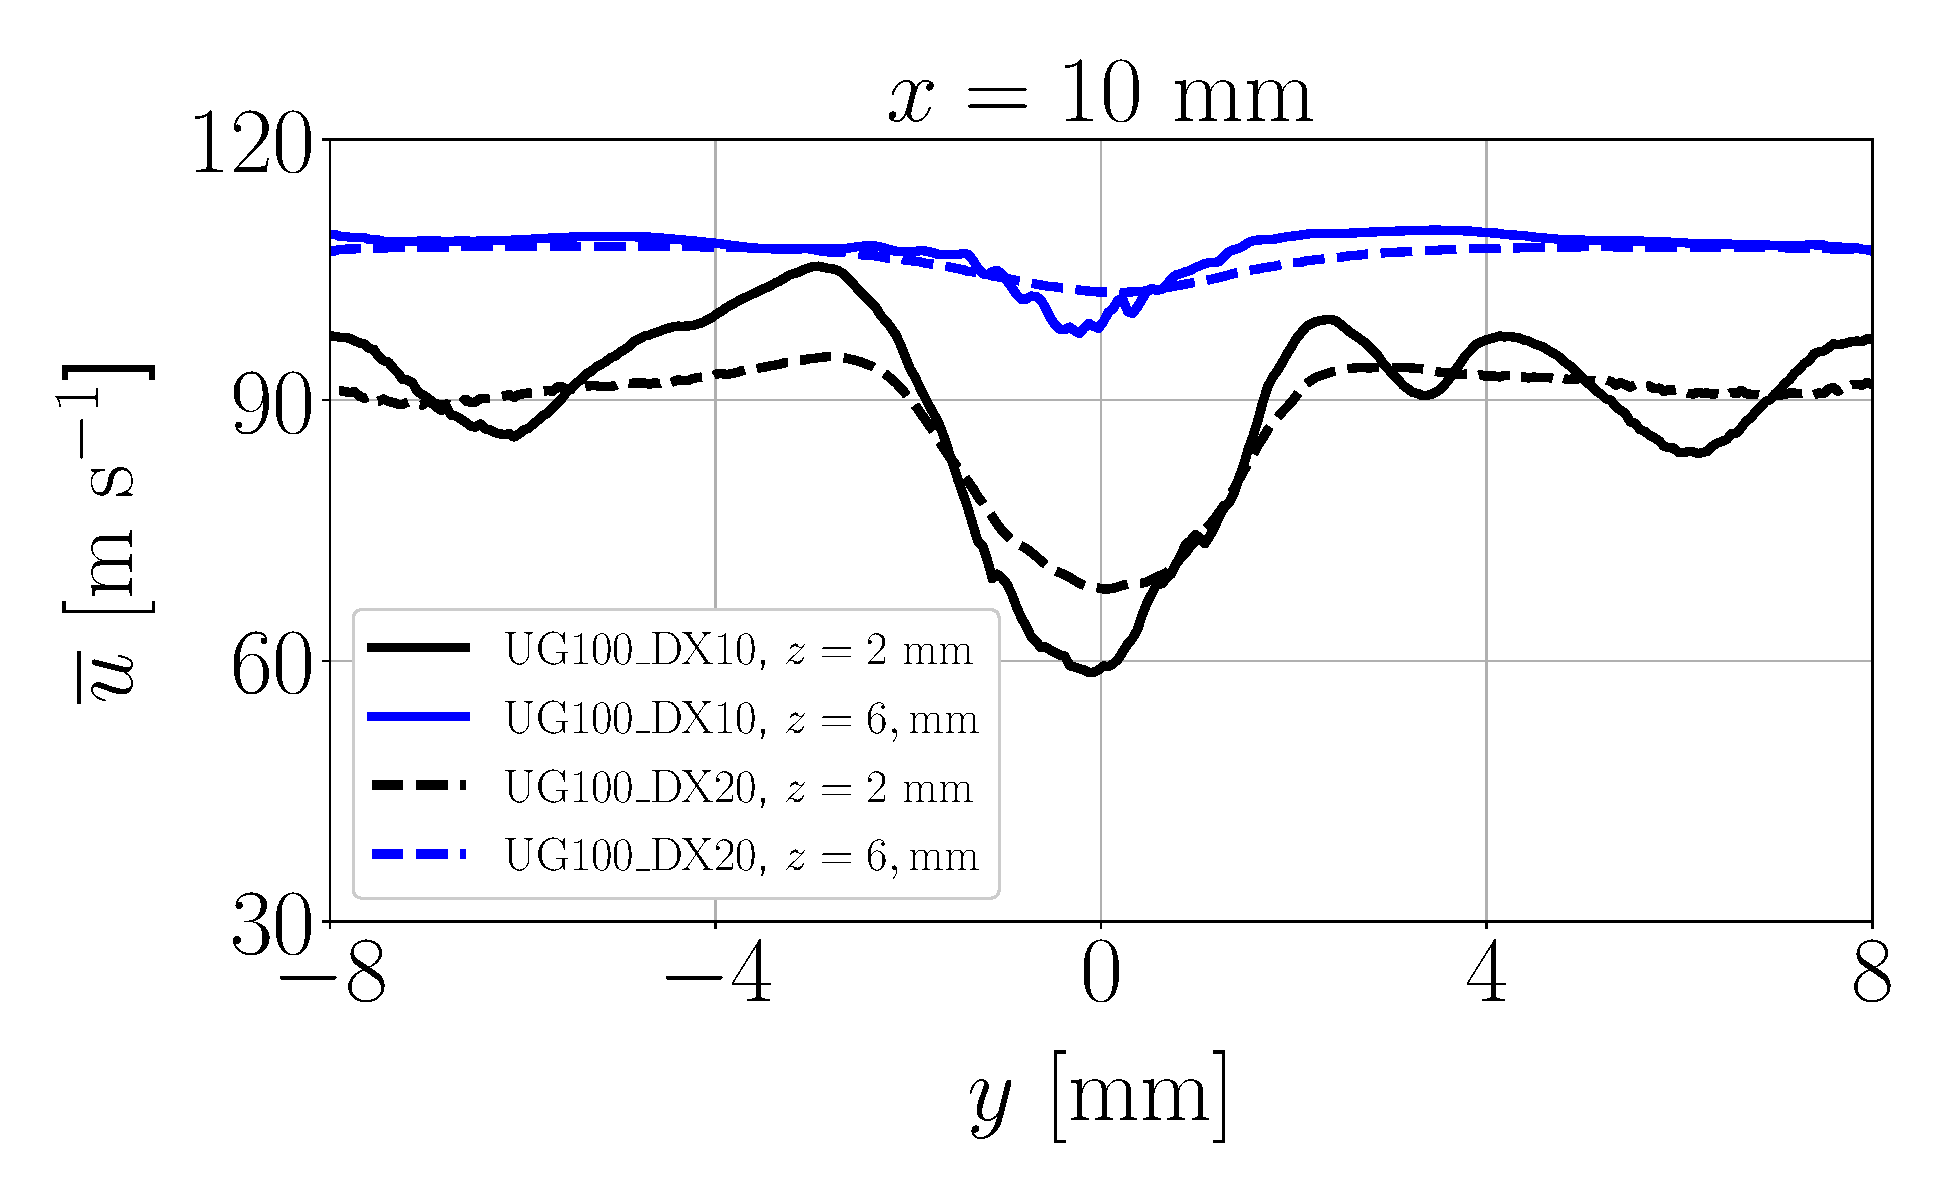
\includegraphics[scale=0.24]{./part2_developments/figures_ch5_resolved_JICF/turbulent_structures/lines_iso-x_along_y_ux_mean_UG100_x10}
   \vspace*{-0.1in}
	\caption{High Weber operating point}
\end{subfigure}
   \caption{Mean axial velocity evolution along lateral coordinate at $z$ lines of Figure \ref{fig:JICF_turbulent_structures_planes_x}}
\label{fig:JICF_sps_lines_iso-x_along_y_ux_mean}
\end{figure}


Finally, the mean velocity at the planes perpendicular to the $z$ axis depicted are shown in Figure \ref{fig:JICF_turbulent_structures_planes_z}.  The mean liquid region defined by $\overline{\psi} > 0.5$ is represented in grey. Close to the wall ($z = 0.2$ mm) the dense core has not yet been deformed by the crossflow and its cross-section is circular. As $z$ increases, the column displaces towards the crossflow direction and its cross-section deforms from a circle to a kidney-shape. The recirculation region increases its maximum axial location $x$ with increasing vertical distance $z$. This is due to the larger deformations of the dense core, since further from the wall the kidney-shape acts like a blunt body. The topology of the fields is similar among operating conditions, yet very sensitive to the interface cell resolution. 

All these results show the complex mean features of the turbulent field induced by the crossflow, and the influence that  interface cell size play into their resolution. The role of the Actuator Line Method (ALM) will be to retrieve these features as accurately as possible in the dispersed-phase simulations of Chapter \ref{ch6:jicf_lgs_simulations}.




\clearpage



\begin{figure}[ht]
\centering
   \includeinkscape[inkscapelatex=false,scale=0.25]{./part2_developments/figures_ch5_resolved_JICF/turbulent_structures/planes_z_ux_mean}
\caption[Mean axial velocity at planes $z = 0.2, 0.8, 16$ mm]{Mean axial velocity at planes $z = 0.2, 0.8, 16$. Black lines with arrows are in-plane mean streamlines; the white solid line indicates the contour $\overline{u} = 0$ which delimites the recirculation bubble. The grey area  indicates the mean liquid region, identifed as $\overline{\psi} > 0.5$. The black-dotted circle indicates the location of the injection nozzle}
\label{fig:JICF_turbulent_structures_planes_z}
\end{figure}



%\subsection{Defining pressure differences}
%\label{ch5:subsec_defining_pressure_differences}

\subsection{Direct measurement of liquid fluxes}
\label{subsec:ch5_direct_measurement_fluxes_IB}

Droplet sampling procedure is performed by tracking the center of mass of resolved structures and retrieving droplets when they cross the defined sampling planes by lagrangian projection. With this tool, some droplets are tracked twice and some others might never be tracked. As a consequence, the sampled spray is not the actual spray that crosses the sampling surfaces in the simulations, but an approximation to it. Therefore, the obtained spray size distributions and sampled mass flow rates are also affected. To check the accuracy of the lagrangian projection procedure, the lagrangian mass flow rates will be compared to flow rates measured directly from the resolved simulations (resolved fluxes). The procedure followed to process these resolved fluxes is detailed in Appendix \ref{app:processing_JICF_IBS}, while here only results are presented. 

The first step is to define the spatial regions where liquid rates will be calculated. For comparison with the lagrangian tracking methodology, fluxes are measured in planes perpendicular to the crossflow direction. Figure \ref{fig:jicf_interior_boundaries_surface_measurements}.  shows a schematic view of the planes, equally spaced at a distance of 5 mm: $x = 5, 10$ and $15$ mm. In simulations where liquid is removed at $x = 11$ mm, only the first two planes will be considered (since there is  no liquid flux through the third one). Furthermore, three more planes are defined parallel to the bottom wall to quantify the liquid flow rate impinging the channel, phenomenon known as filming: $x < 5, 10$ and 15 mm. Therefore, each combination of sampling and filming surfaces will conform the outlet surfaces of a control volume enclosing the whole liquid jet (no outlet surfaces are located upstream the injection point as there is no liquid flowing in this direction, and the inlet surface corresponds to the liquid
nozzle). Each plane where resolved fluxes are calculated will be hereafter referred as interior boundary (IB).

\clearpage

\begin{figure}[ht]
     \centering
     \includeinkscape[inkscapelatex=false,scale=0.4]{./part2_developments/figures_ch5_resolved_JICF/sampling_planes_with_IBs}
     \caption{Snapshot of a JICF simulation showing the droplets sampling planes (in grey) and the different filming regions}
	% See: https://stackoverflow.com/questions/35210337/can-i-plot-several-histograms-in-3d/35225919
      \label{fig:jicf_interior_boundaries_surface_measurements}
\end{figure}

Figure \ref{fig:IB_liquid_flow_rate_inst_evolution_UG100_DX10} shows an example of instantaneous liquid flow rates $Q_l$ from case UG100\_DX10. Two IBs perpendicular to the $x$ axis ($x = $ 5, 10 mm) are tracked in the left image, and two filming IBs ($x < $ 5, 10 mm) are displayed in the right one. The fluxes in Figure \ref{fig:IB_liquid_flow_rate_inst_evolution_UG100_DX10} left show a high variation around the injected flux in both planes. This is due to an intermittent presence of liquid crossing the sampling planes once atomization has started taken place: the liquid phase is no longer a coherent jet but is composed by an ensemble of ligaments and droplets. At some instants there are large clusters of droplets or large ligaments crossing the domain (large fluxes), while in other cases there might only be a few droplets being sampled (low fluxes). Regarding filming, these present lower magnitudes but still display an oscillating behaviour which, in some cases, can descend up to $0$ (no liquid impinging the wall).


\begin{figure}[ht]
\flushleft
\begin{subfigure}[b]{0.45\textwidth}
	\centering
   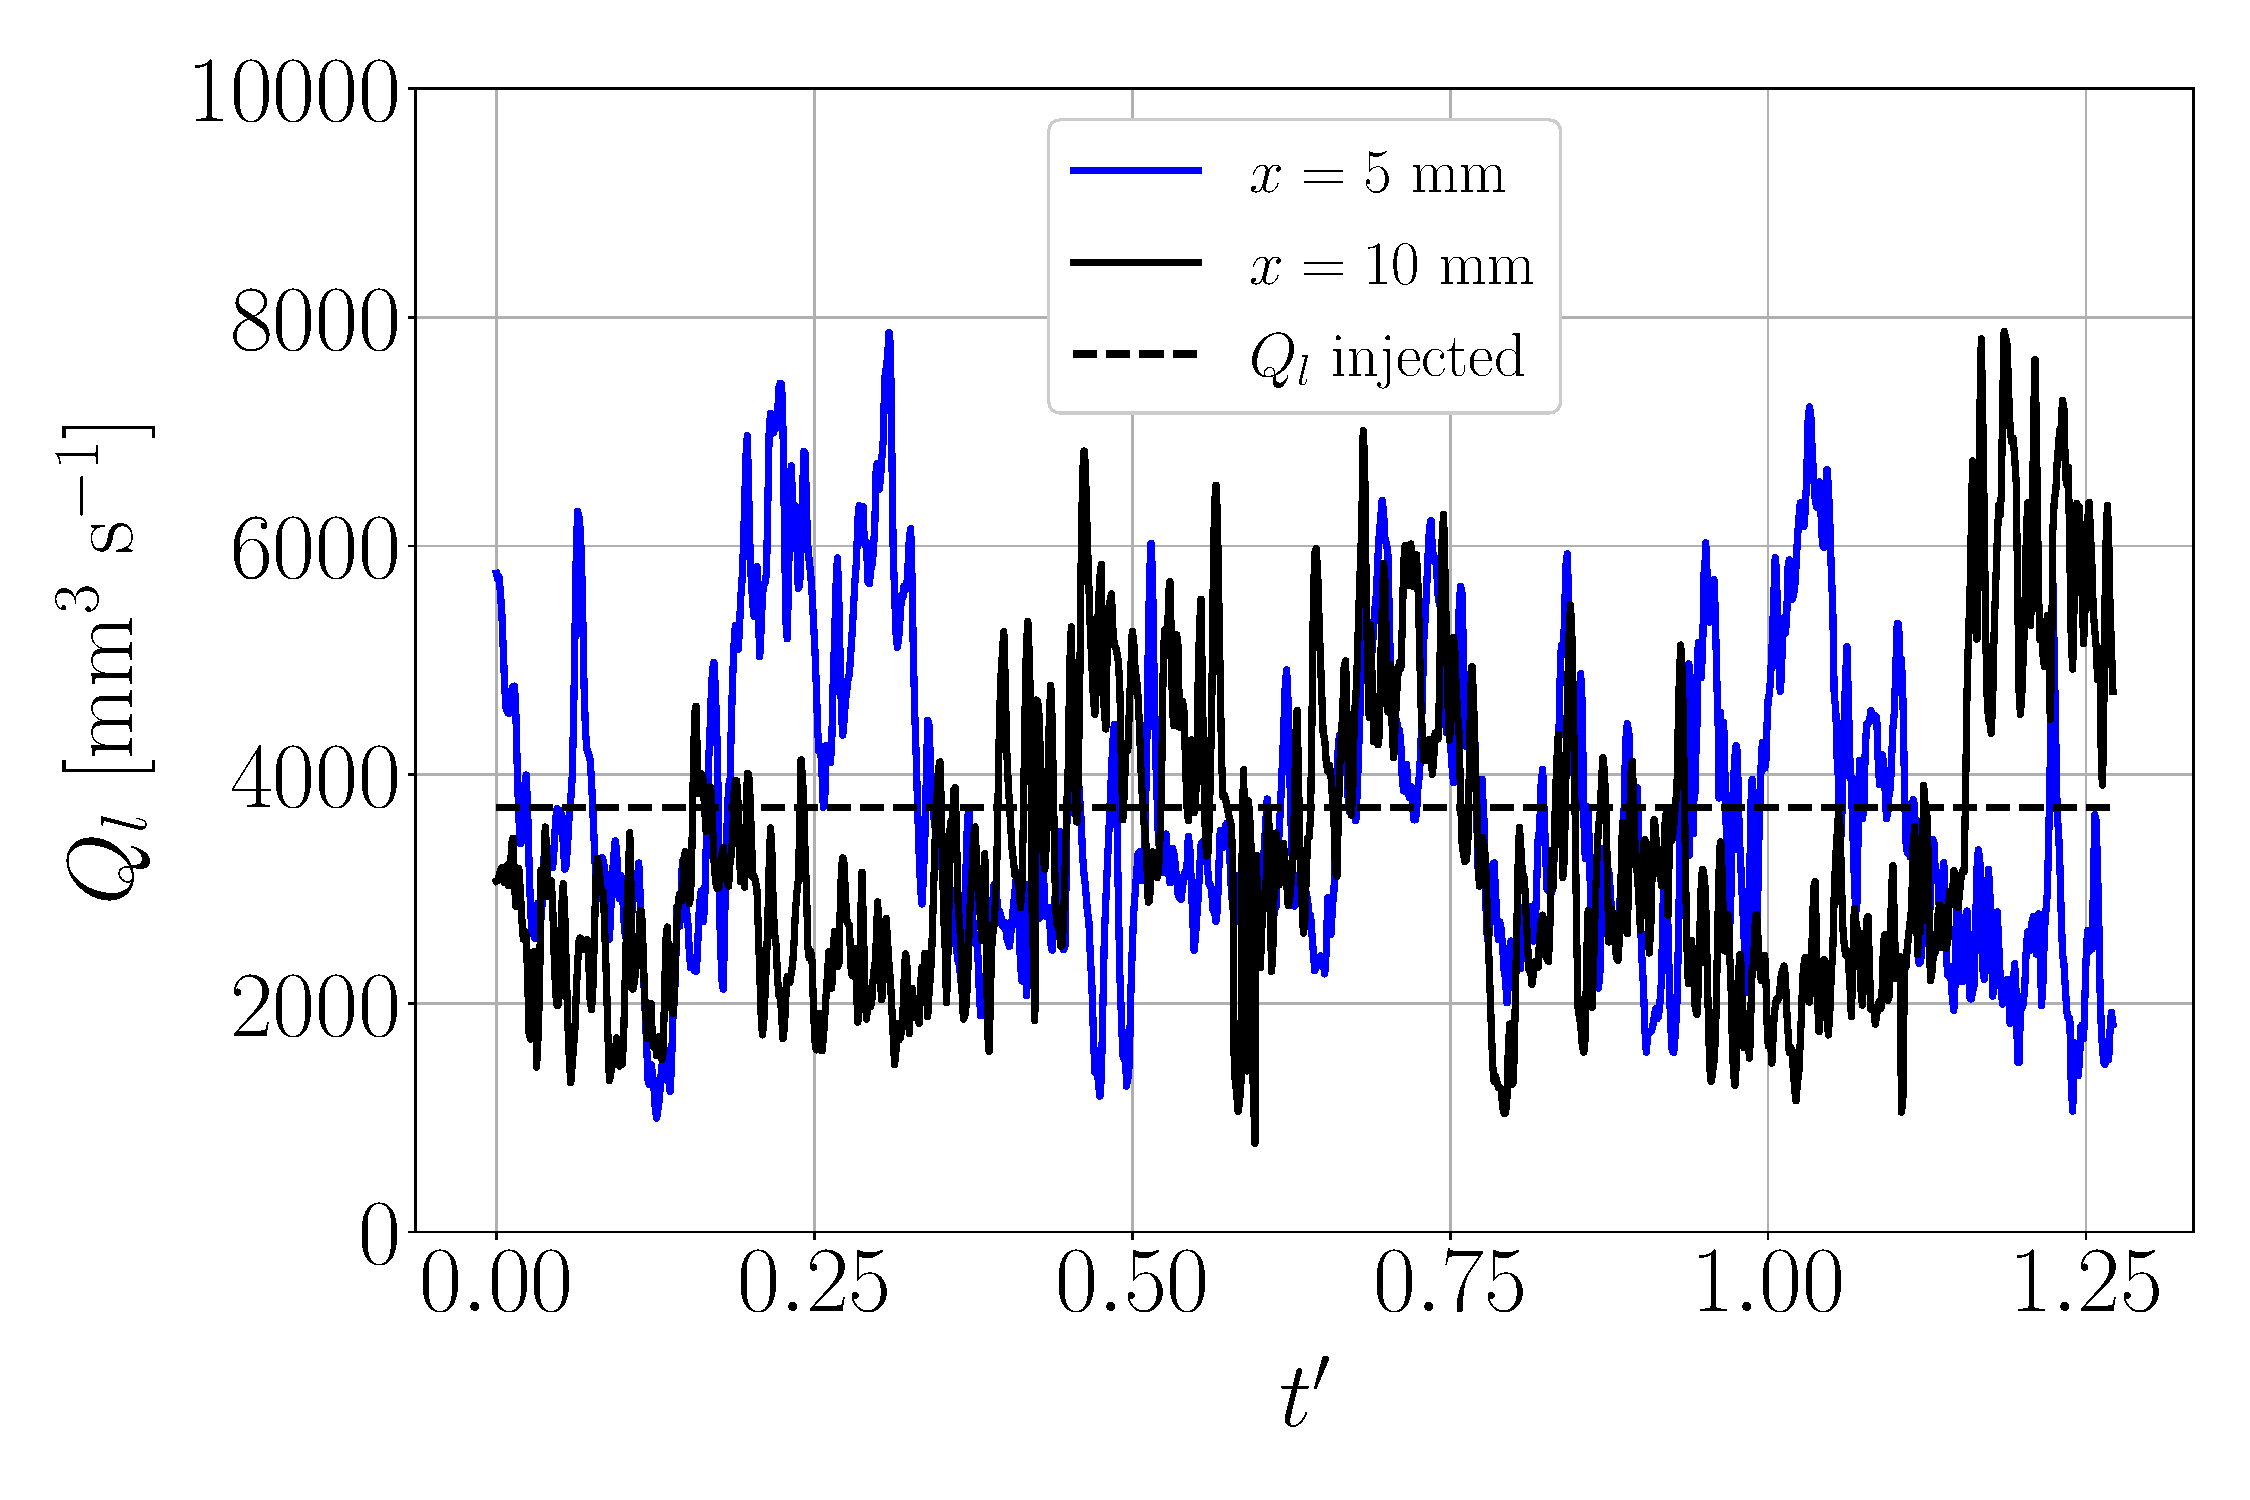
\includegraphics[scale=0.222]{./part2_developments/figures_ch5_resolved_JICF/flow_rates_ibs/inst_Q_iso_x_UG100_dx10}
   %\caption{}
   %\label{} 
\end{subfigure}
\hspace{0.4in}
\begin{subfigure}[b]{0.45\textwidth}
	\centering
   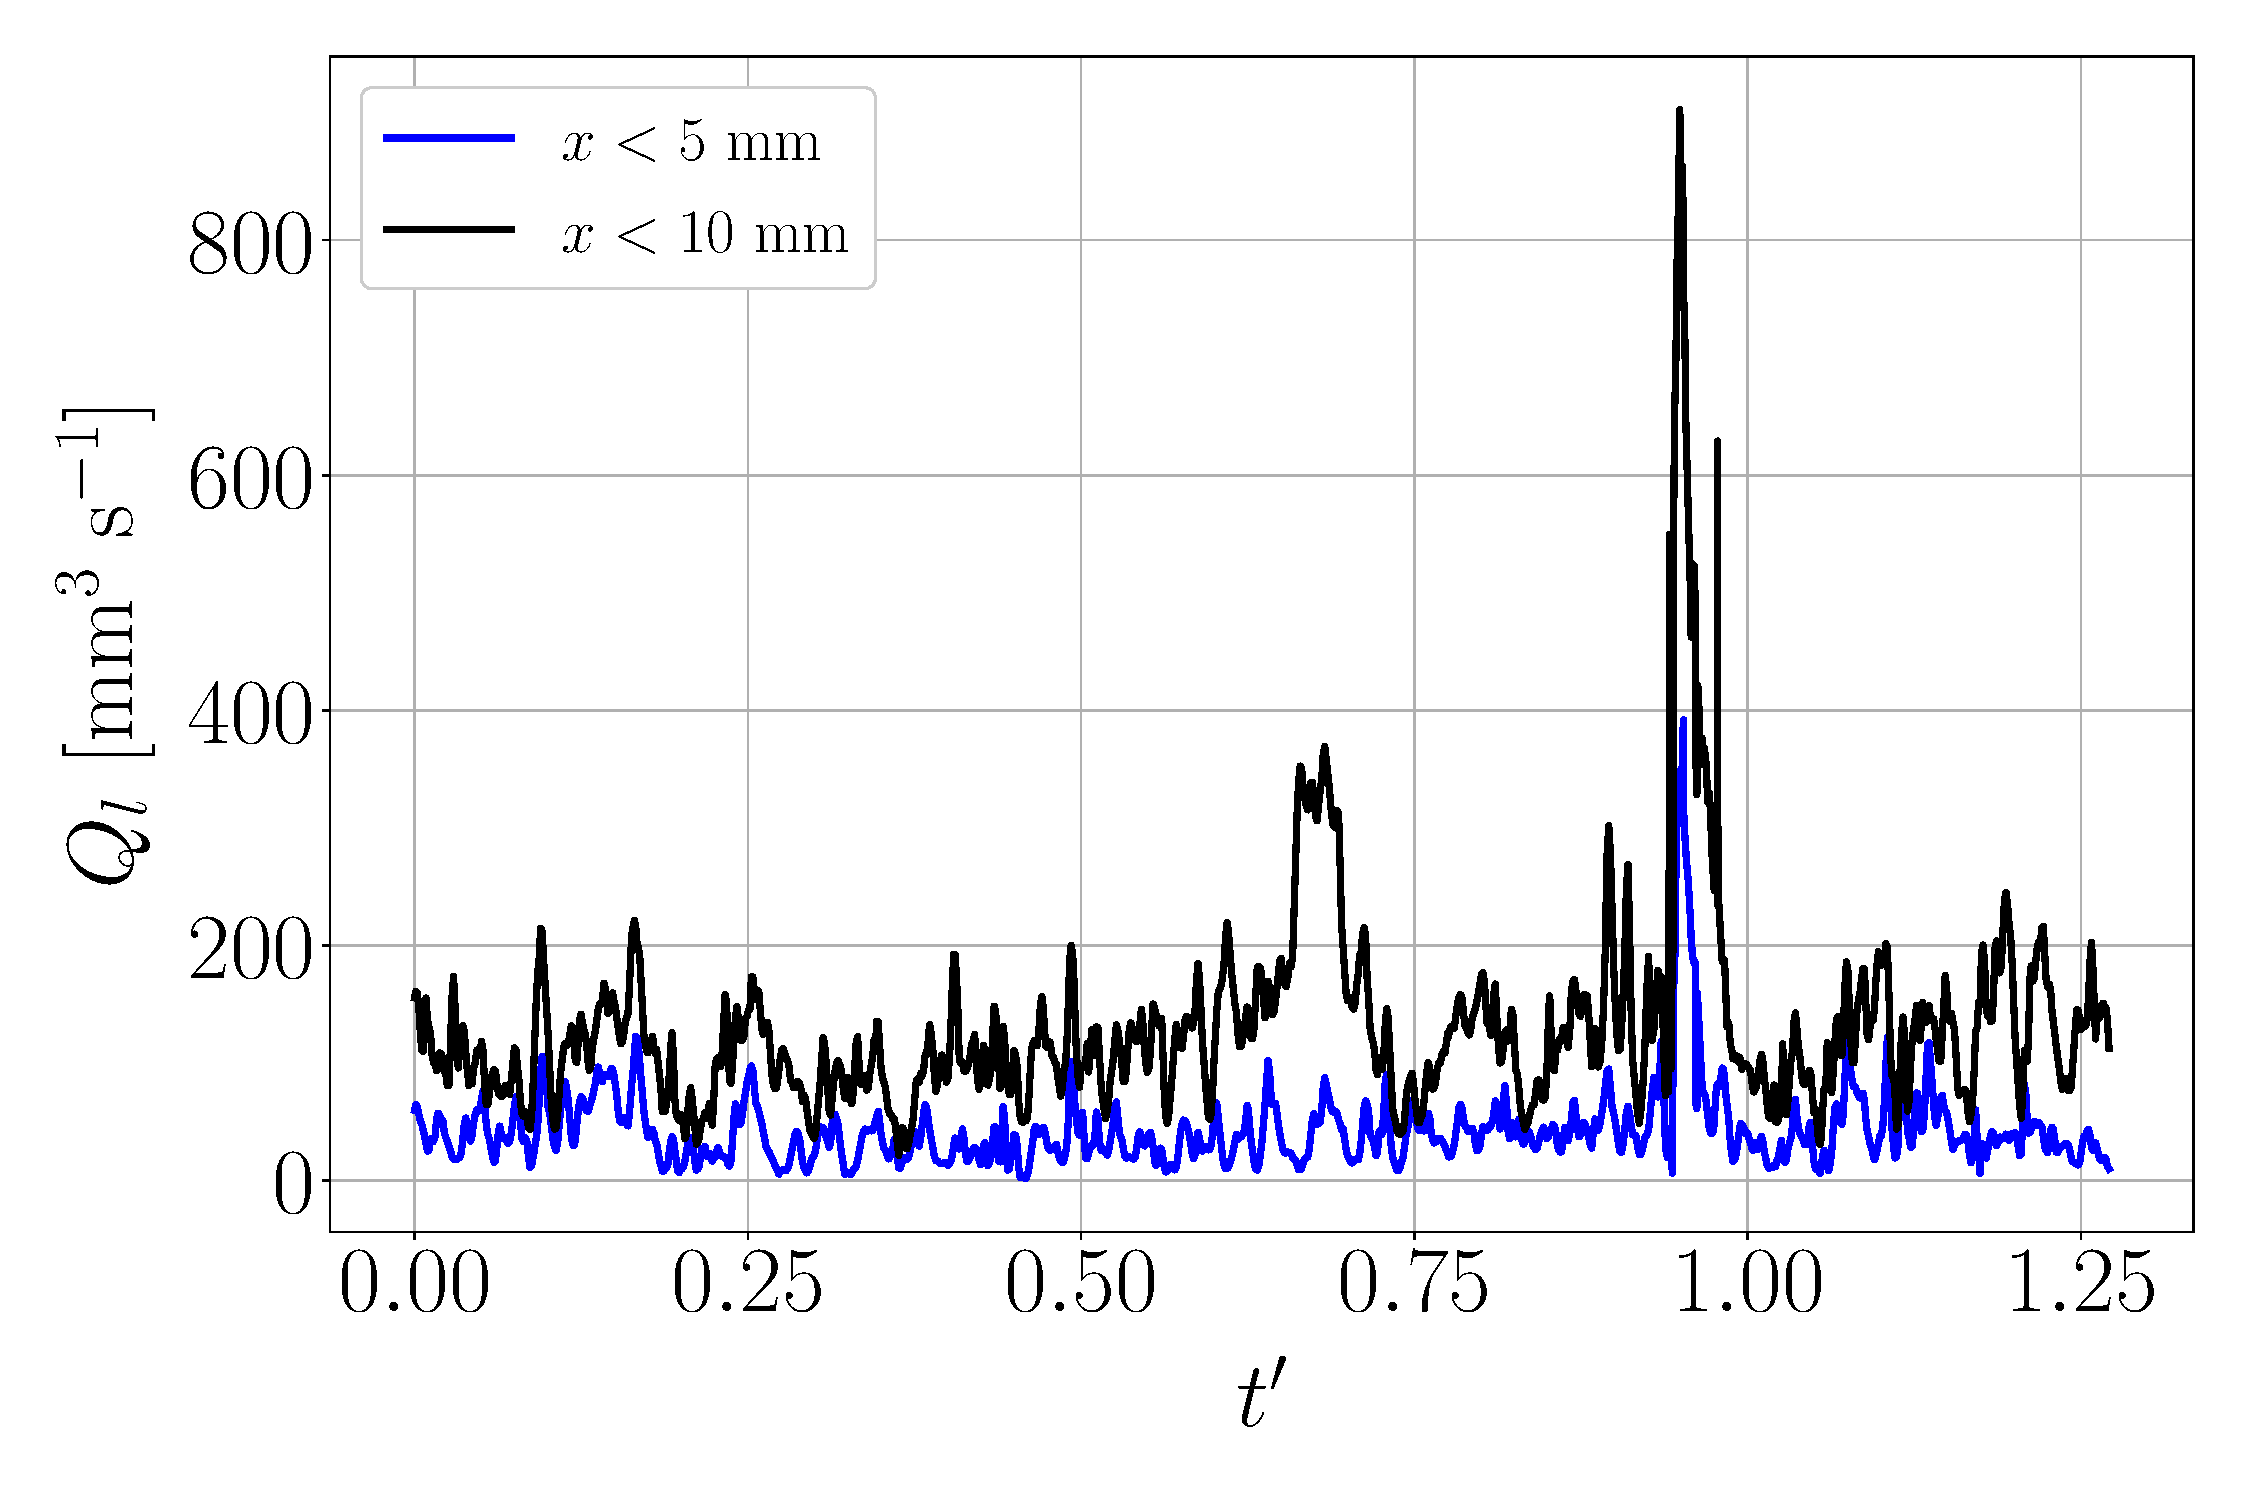
\includegraphics[scale=0.222]{./part2_developments/figures_ch5_resolved_JICF/flow_rates_ibs/inst_Q_iso_x_UG100_dx10_filming}
   %\caption{}
   %\label{}
\end{subfigure}
   \vspace*{-0.20in}
\caption[Time evolution of instantaneous liquid flow rates $Q_l$ for case UG100\_DX10.]{Time evolution of instantaneous liquid flow rates $Q_l$ for case UG100\_DX10. \textsl{Left}: planes normal to crossflow. \textsl{Right}: filming planes.}
\label{fig:IB_liquid_flow_rate_inst_evolution_UG100_DX10}
\end{figure}

Due to the intermittent behaviour of the jet downstream the injection nozzle, the instantaneous fluxes are not useful to characterize the flow rates in the IBs. Instead, the mean and RMS fluxes provide useful information on the mass conservation in the JICF. The evolution of the mean and RMS values of IBs flow rates with time is shown in Figure \ref{fig:IB_mean_RMS_Ql_evolution}. Statistics have been taken for $t^{\prime} > 2$ in all cases. The evolution of $\overline{Q}_l$ in the perpendicular IBs (Figure \ref{fig:IB_mean_RMS_Ql_evolution}a) shows that all cases tend towards convergence: the fine cases are shown to be completely converged, while the fine ones show some oscillations at the last timesteps sampled but with a lower amplitude, indicating that they are almost converged. In all cases, the mean values for perpendicular IBS are reduced downstream the crossflow, while the mean filming ones are increased. The RMS values of Figure \ref{fig:IB_mean_RMS_Ql_evolution}b show high magnitudes caused by the high fluctuations in the flow rates as illustrated in Figure \ref{fig:IB_liquid_flow_rate_inst_evolution_UG100_DX10}a, which are present in all cases. The steep increases in the RMS at certain times is due to a high volume of liquid crossing the IB at the corresponding instant.%, as previously discussed before when commenting Figure \ref{fig:IB_liquid_flow_rate_inst_evolution_UG100_DX10}.


\clearpage


\begin{figure}[ht]
\flushleft
\begin{subfigure}[b]{0.9\textwidth}
	\flushleft
   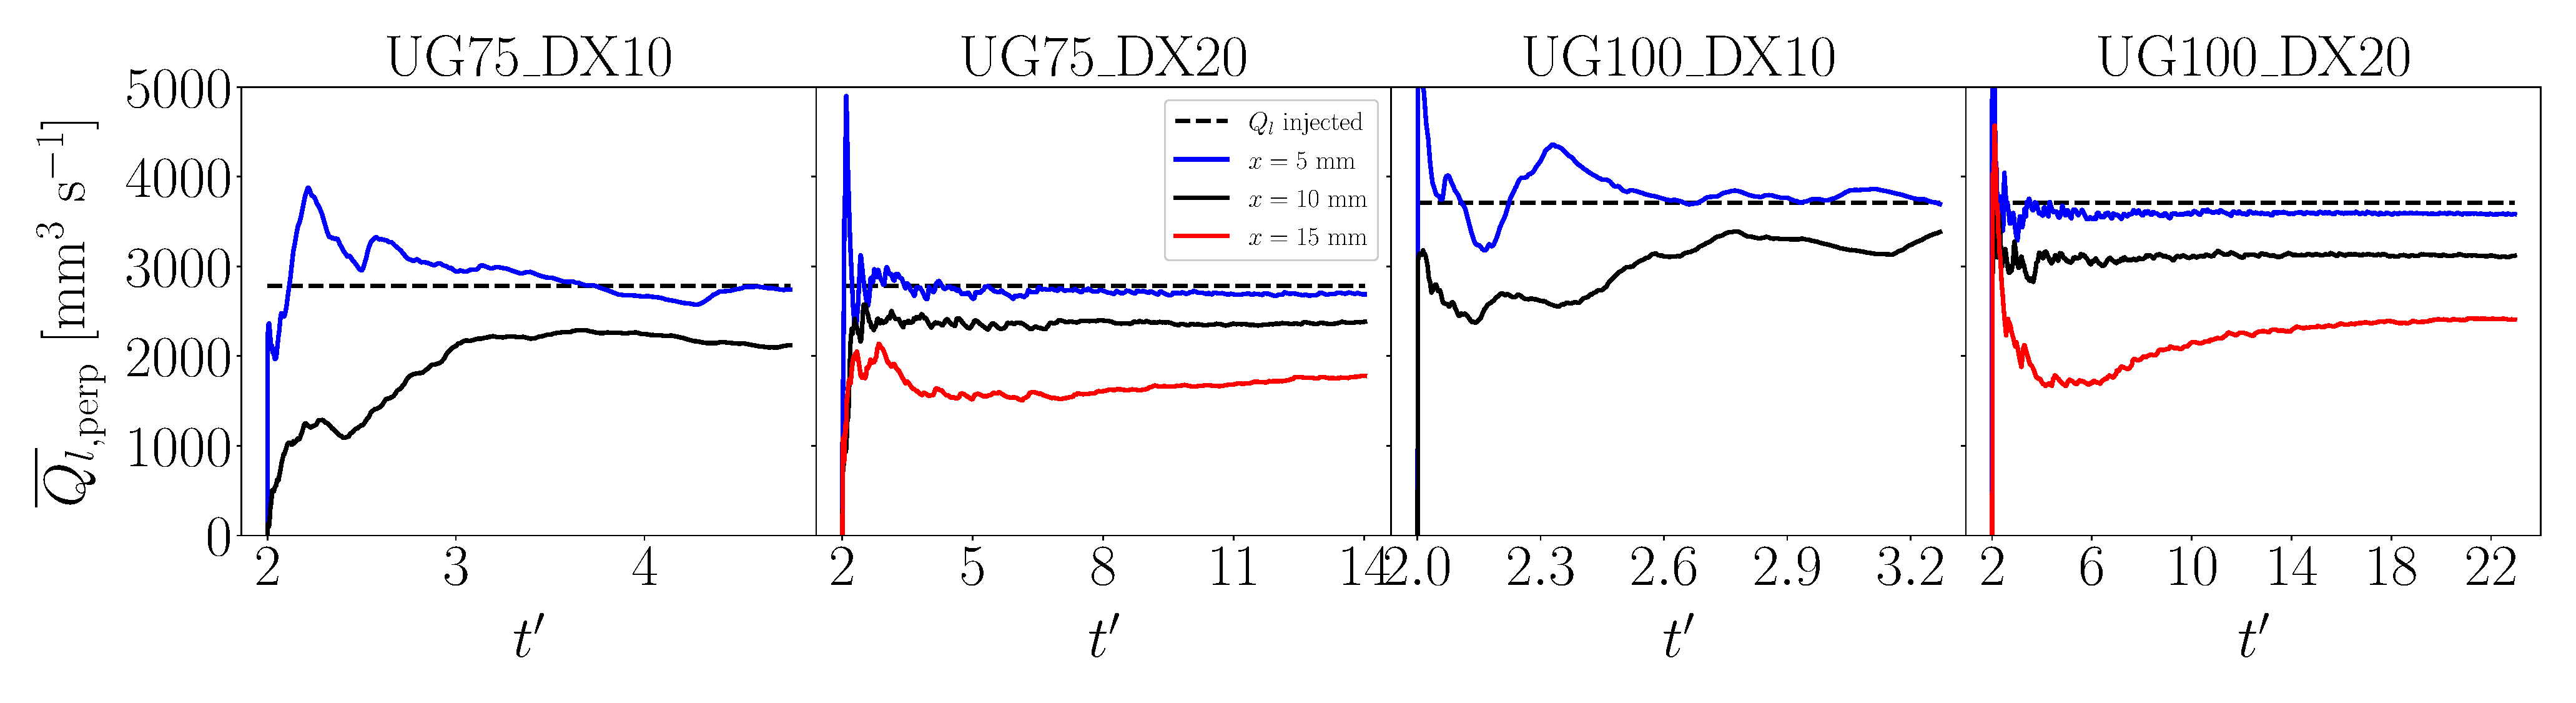
\includegraphics[scale=0.25]{./part2_developments/figures_ch5_resolved_JICF/flow_rates_ibs/evolution_mean_Q_iso_x}
   \vspace*{-0.25in}
   \caption{Mean $Q_l$ evolution in IBs perpendicular to crossflow.}
   %\label{} 
\end{subfigure}

\vskip\baselineskip

\begin{subfigure}[b]{0.9\textwidth}
	\flushleft
   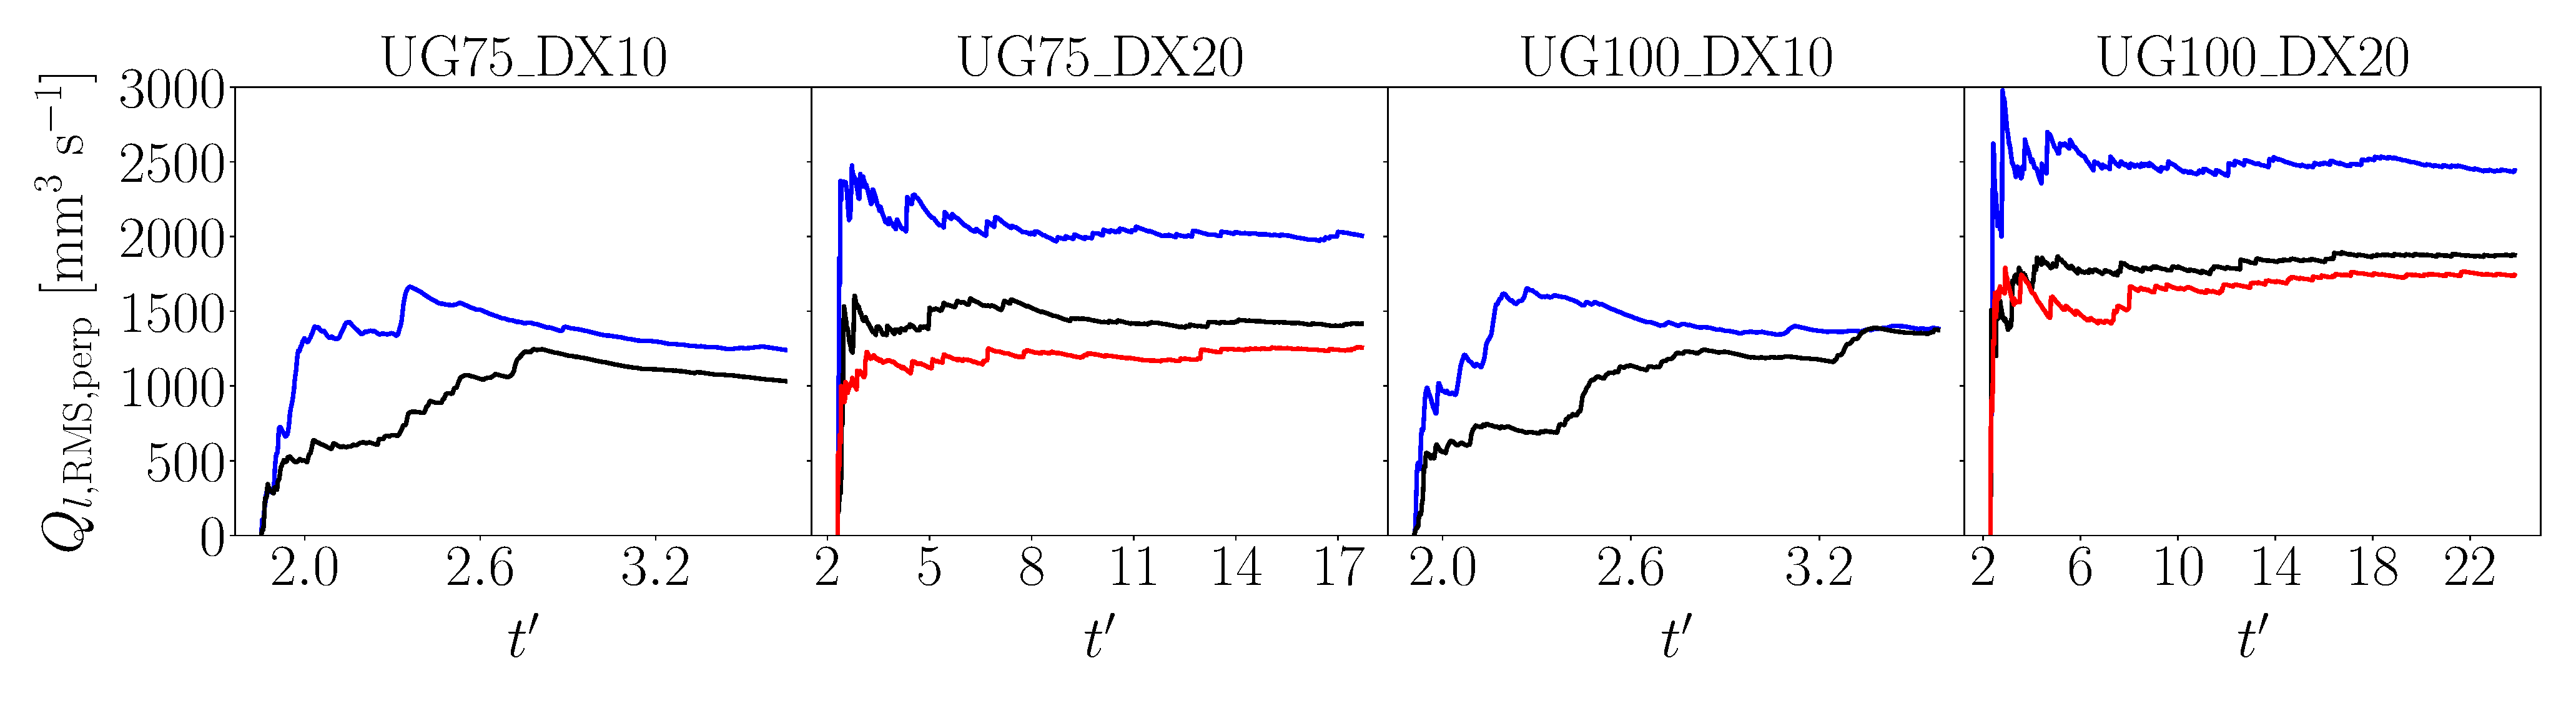
\includegraphics[scale=0.25]{./part2_developments/figures_ch5_resolved_JICF/flow_rates_ibs/evolution_rms_Q_iso_x}
   \vspace*{-0.25in}
   \caption{RMS $Q_l$ evolution in IBs perpendicular to crossflow.}
   %\label{}
\end{subfigure}

\vskip\baselineskip

\begin{subfigure}[b]{0.9\textwidth}
	\flushleft
   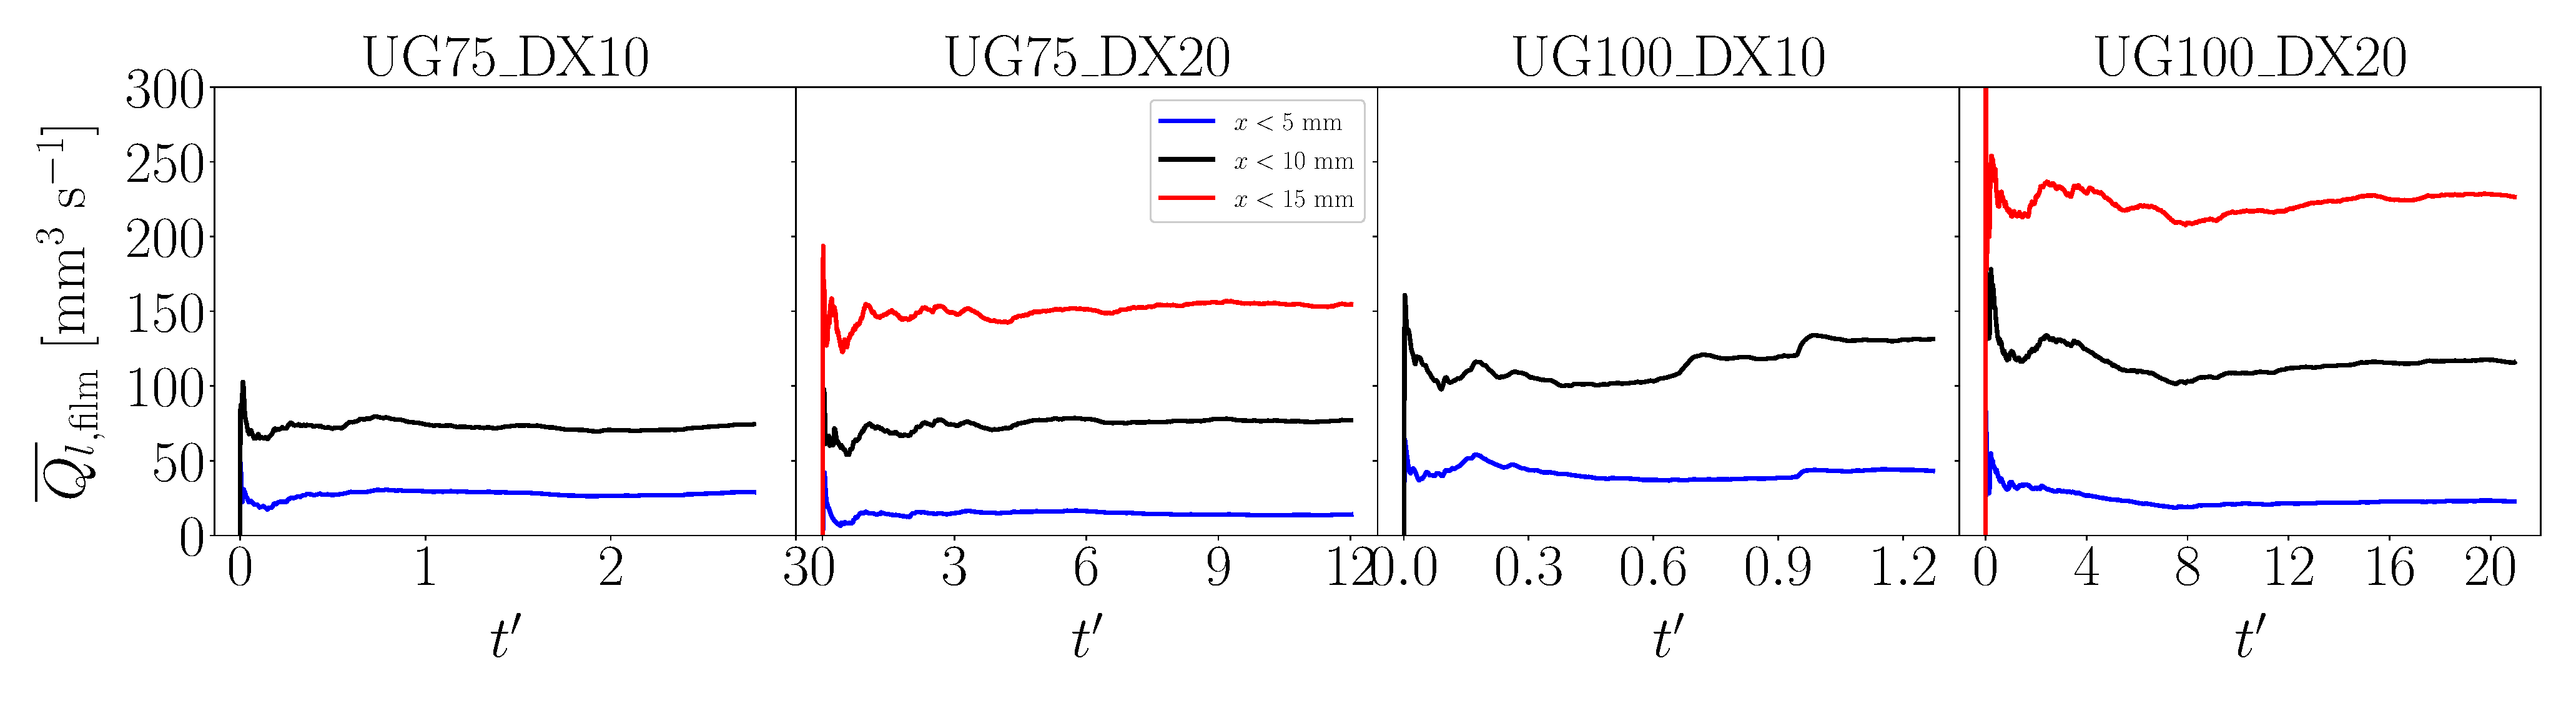
\includegraphics[scale=0.25]{./part2_developments/figures_ch5_resolved_JICF/flow_rates_ibs/evolution_mean_Q_filming}
   \vspace*{-0.25in}
   \caption{Mean $Q_l$ evolution in filming IBs.}
   %\label{} 
\end{subfigure}

\vskip\baselineskip

\begin{subfigure}[b]{0.9\textwidth}
	\flushleft
   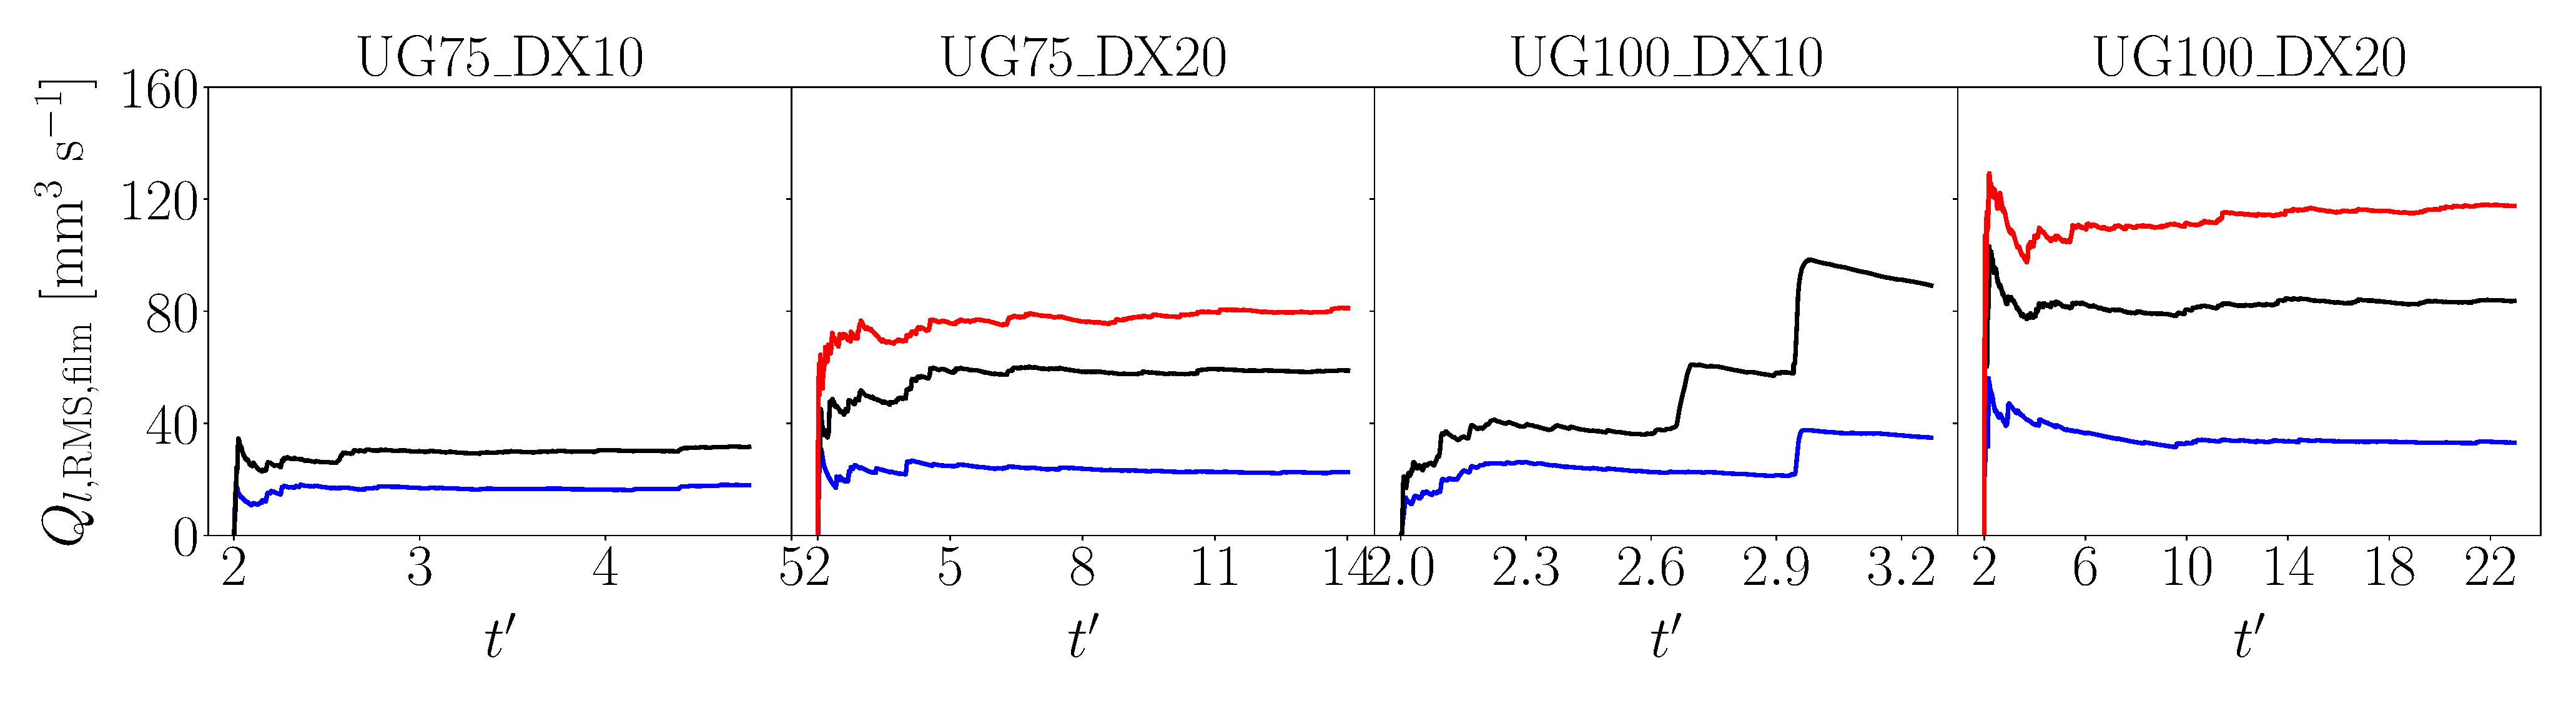
\includegraphics[scale=0.25]{./part2_developments/figures_ch5_resolved_JICF/flow_rates_ibs/evolution_rms_Q_filming}
   \vspace*{-0.25in}
   \caption{RMS $Q_l$ evolution in filming IBs.}
   %\label{}
\end{subfigure}
\caption{Time evolution of mean and RMS values of $Q_l$ in IBs}
\label{fig:IB_mean_RMS_Ql_evolution}
\end{figure}

\clearpage


\begin{figure}[ht]
\centering
\begin{subfigure}[b]{0.9\textwidth}
	\centering
   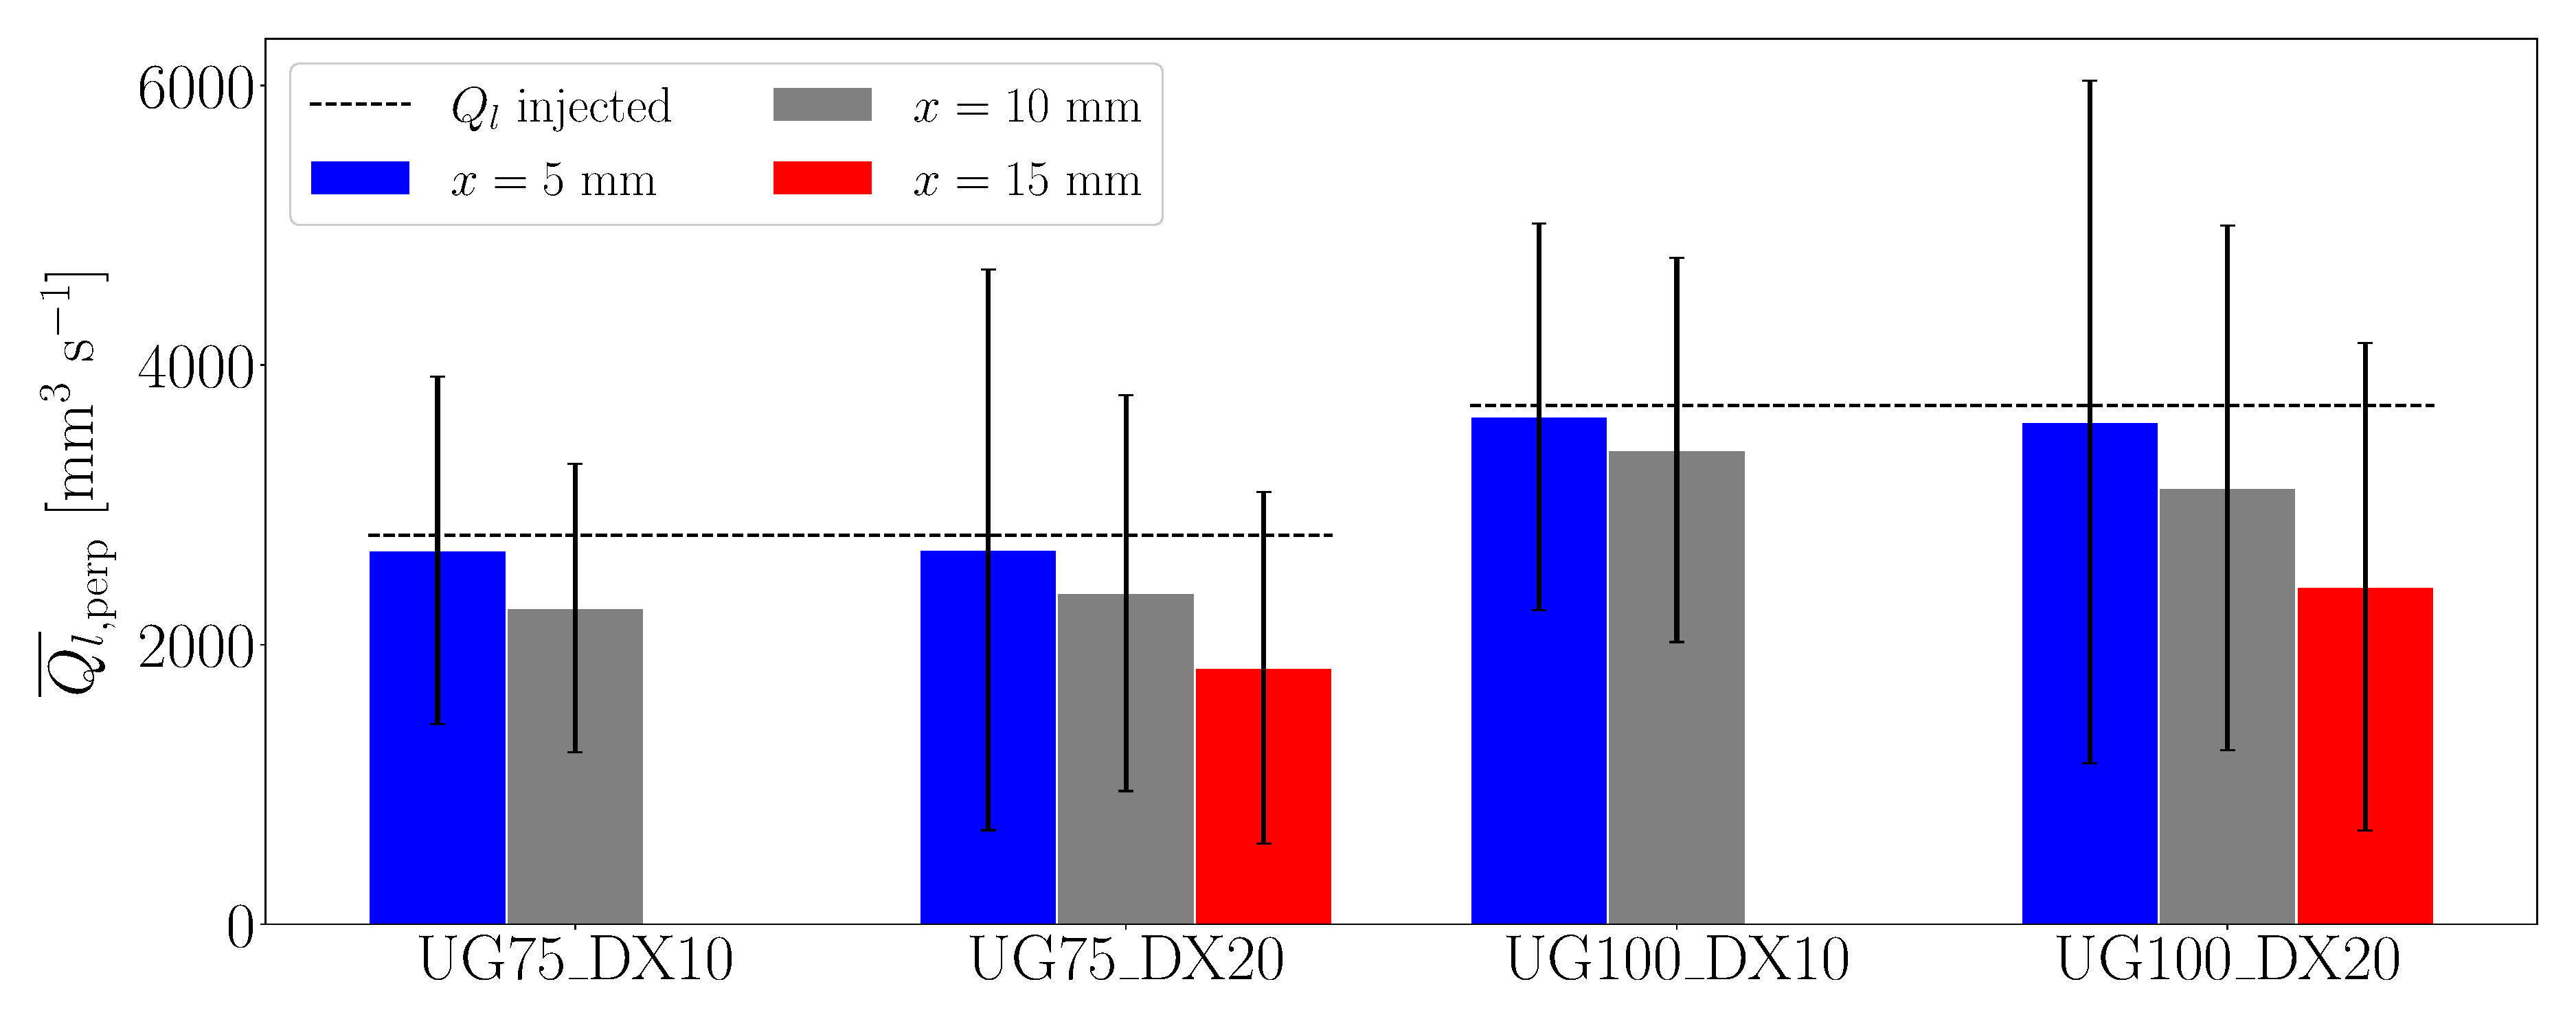
\includegraphics[scale=0.225]{./part2_developments/figures_ch5_resolved_JICF/flow_rates_ibs/bar_graph_isox_IBs}
   \caption{IBs perpendicular to crossflow.}
   \label{fig:IB_bargraph_perp}
\end{subfigure}

\vskip\baselineskip

\begin{subfigure}[b]{0.9\textwidth}
	\centering
   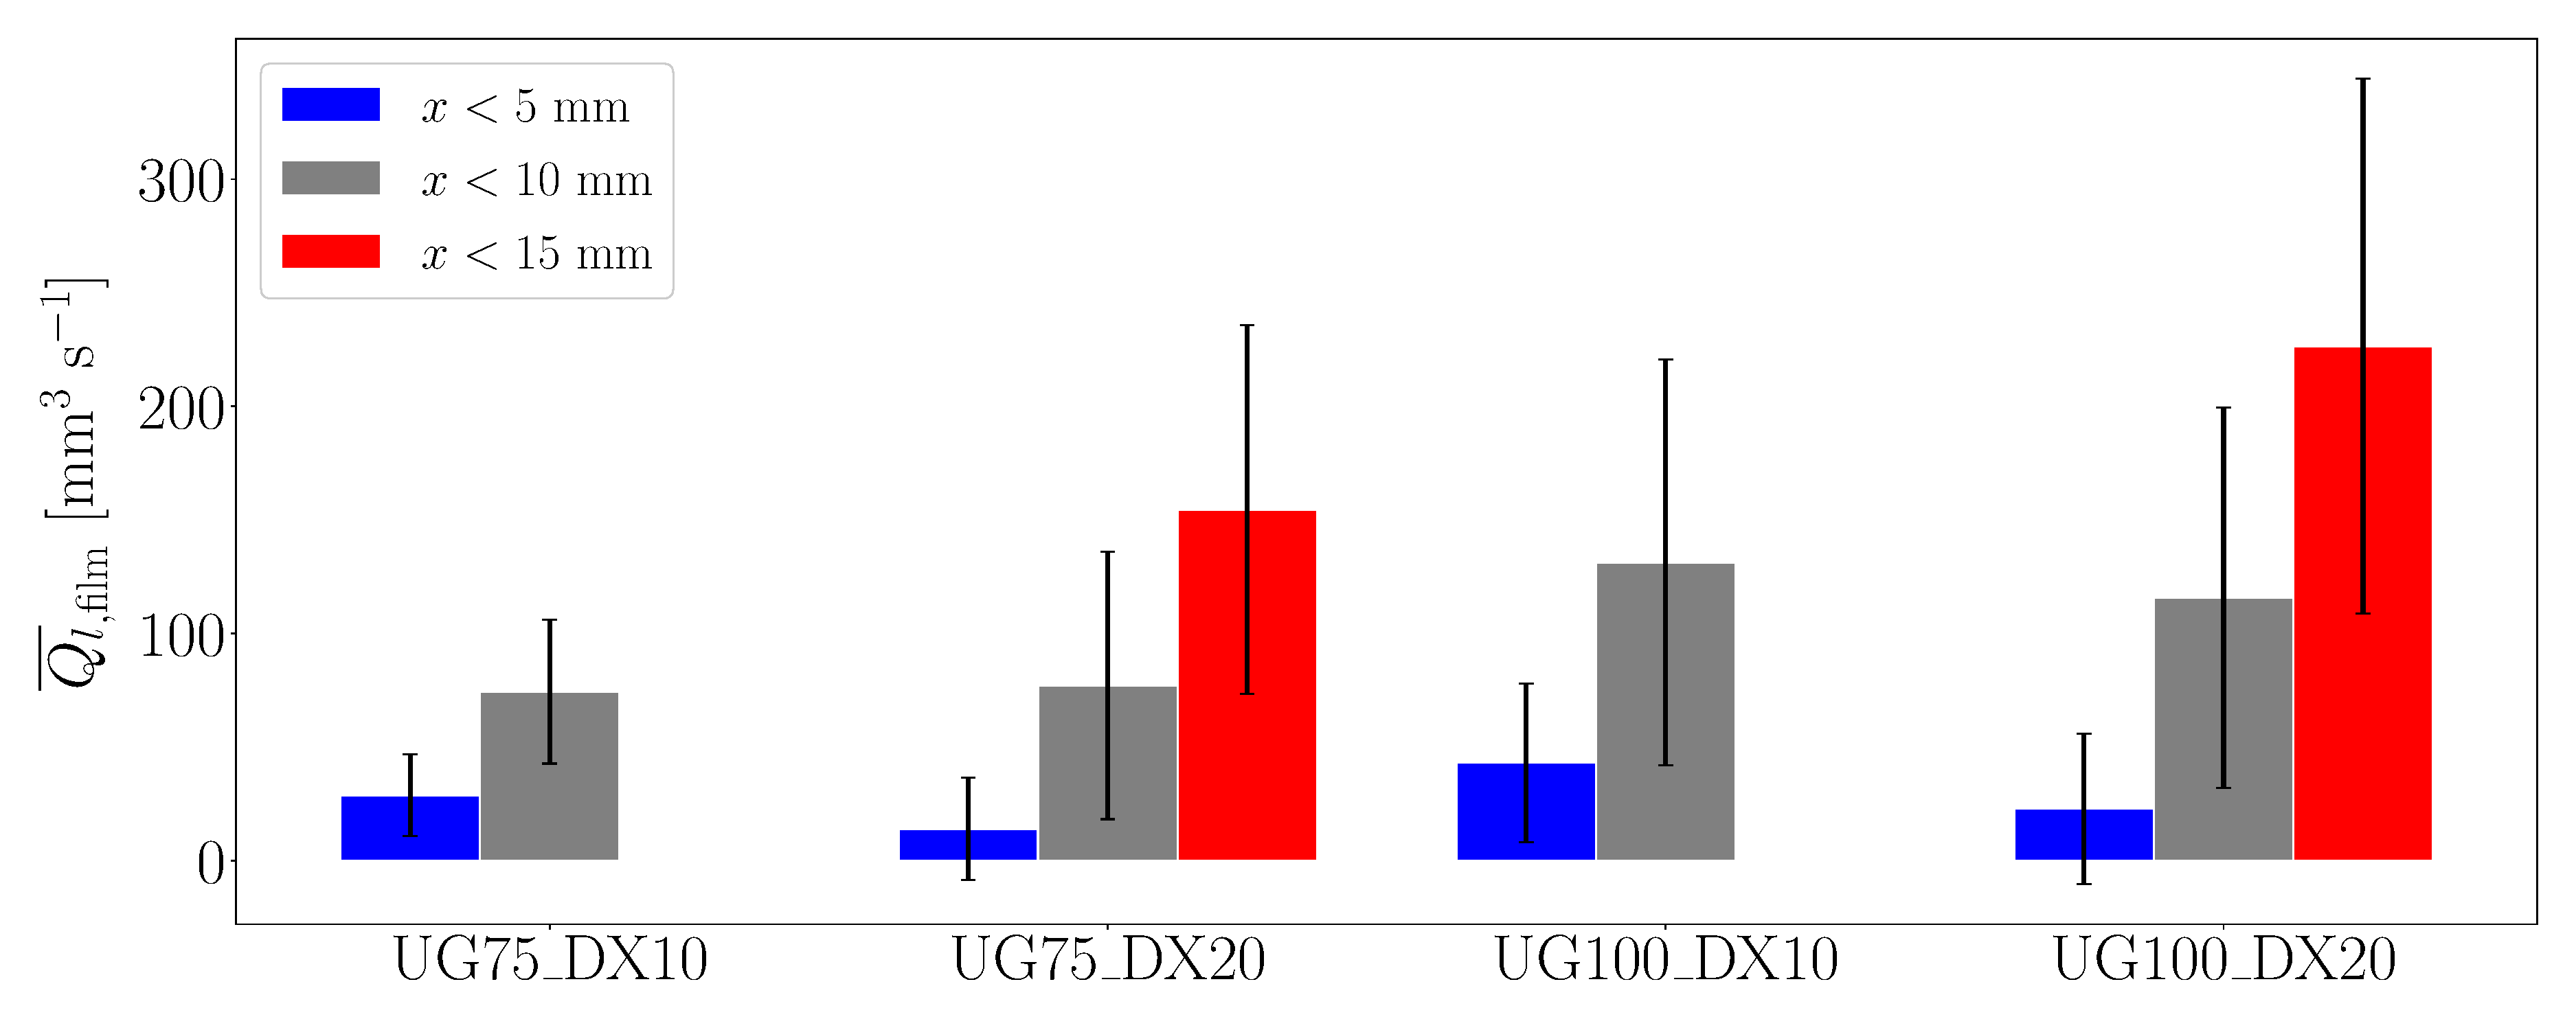
\includegraphics[scale=0.225]{./part2_developments/figures_ch5_resolved_JICF/flow_rates_ibs/bar_graph_filming_IBs}
   \caption{Filming IBs.}
   \label{fig:IB_bargraph_filming}
\end{subfigure}

\vskip\baselineskip

\begin{subfigure}[b]{0.9\textwidth}
	\centering
   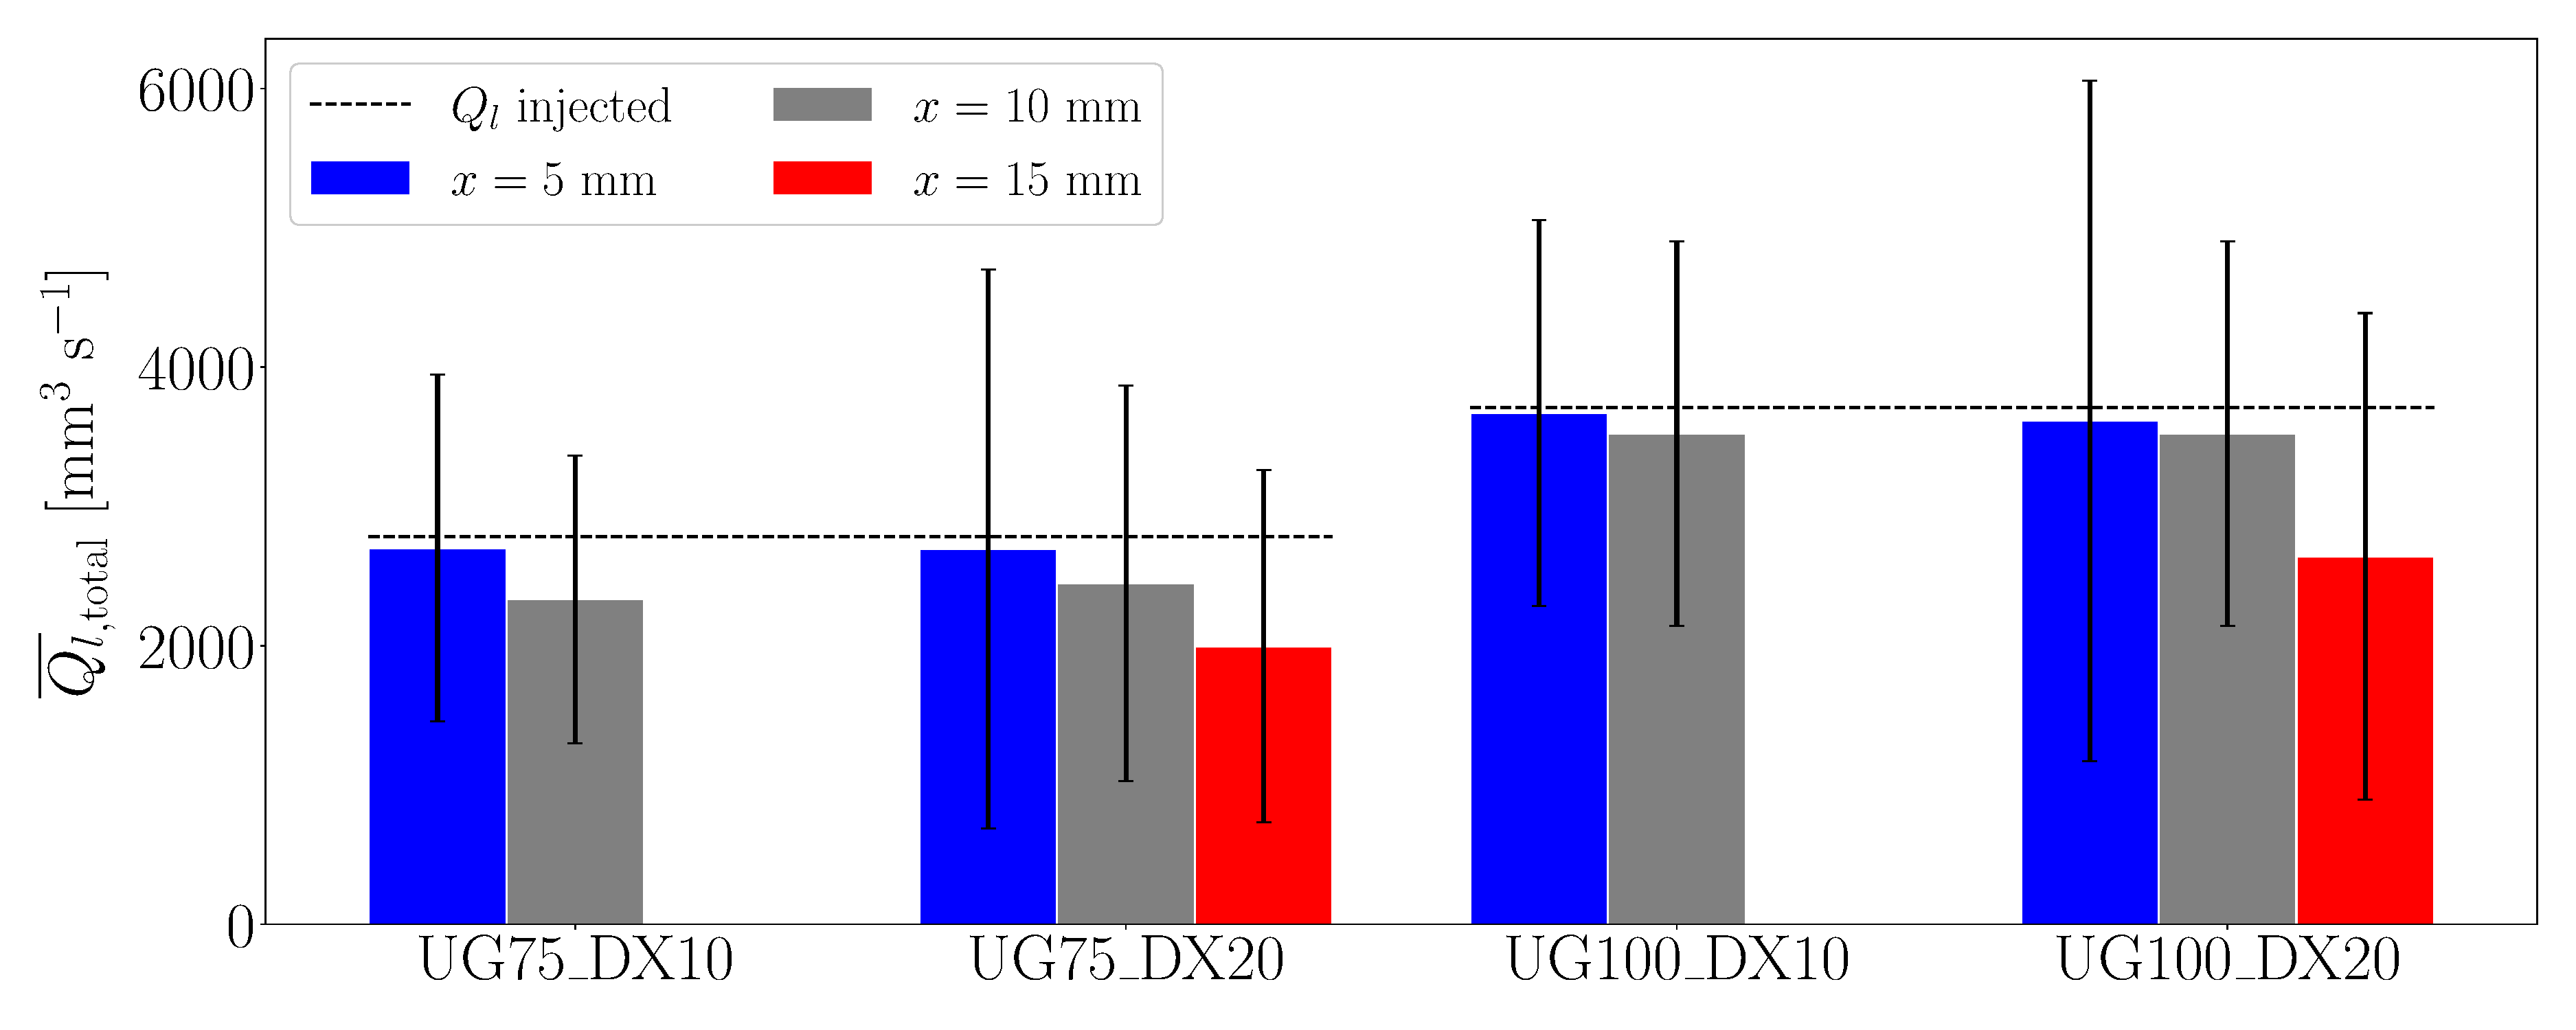
\includegraphics[scale=0.225]{./part2_developments/figures_ch5_resolved_JICF/flow_rates_ibs/bar_graph_total_IBs}
   \caption{Total (perpendicular + filming) flow rates from IBs}
   \label{fig:IB_bargraph_total}
\end{subfigure}
\caption{Mean flow rates (bars) and RMS (black vertical lines) obtained with IBs for each simulation.}
\label{fig:IB_bargraph}
\end{figure}

\clearpage

Figure \ref{fig:IB_bargraph} shows the final mean and RMS values for the flow rates. Three graphs are represented: (a) the IBs perpendicular to the crossflow direction, (b) the filming IBs and (c) the addition of both filming and perpendicular IBs at each location, named total flux:

\vspace*{-0.1in}

\begin{equation}
\overline{Q_l}_{\mathrm{total}} = \overline{Q_l}_{\mathrm{film}} + \overline{Q_l}_{\mathrm{perp}}
\end{equation}

In the JICF configuration studied, if an arbitrary cubic control volume is located englobing the jet and spray, liquid mass can leave this domain only through either the perpendicular or filming surfaces. Since the plenum domain is large enough to avoid liquid impinging the top and side walls, only these two rates comprise the liquid outlets. Therefore, the total flux should ideally equal the injected flow rate. %(the only liquid inlet in the system) due to mass conservation. 

Figures \ref{fig:IB_bargraph}a and b show that perpendicular fluxes decrease with axial distance, while filming ones increase. This is coherent, since droplets that cross a perpendicular IB closer to the injector might then reach the wall before reach the following (i.e. the one located 5 mm downstream) perpendicular one, hence contributing to the filming flux instead. Nevertheless, Figure \ref{fig:IB_bargraph}c shows that the total flow rate is not conserved with axial distance, but actually decreases in all simulations: mass is lost in the simulations. Liquid mass loss can be quantified by substracting the total flow rates from the IBs to the injected flow rate in each simulation. To eliminate this dependence from the operation point, each one with different injected rates, a relative mass loss is defined according to the following formula:


\vspace*{-0.05in}
\begin{equation}
\Delta Q_l = \frac{Q_{l,\mathrm{injected}} - \overline{Q_l}_{\mathrm{total}}}{Q_{l,\mathrm{injected}}}
\end{equation}




Results are shown in Figure \ref{fig:delta_Ql_with_x}. The mass loss is low closer to the injector ($x = 5$ mm), with all values below $3~\%$, then losses increase further downstream.  At the location $x = 15$ mm the relative flow rate loss for the coarse cases is close to $30~\%$: from $x = 10$ to $15$ mm, the mass loss doubles. Indeed, it was found that mass loss is caused by droplets disappearing when reaching a characteristic size of the order of the interface resolution $\Delta x_\mathrm{min}$, since these cannot be further transported by the mesh (see, for instance, droplets generated by surface breakup in Figure \ref{fig:jicf_surface_breakup_ug75_dx10}). Then, for $x > 10$ mm the spray is fully disperse and secondary atomization is taking place: droplets generated might reach a small size and vanish. These values of liquid losses show that the location $x = 5$ mm is more suitable for performing lagrangian injection in the dispersed-phase simulations, since the total liquid flow rated injected is closer to the injected one. A more thorough study on the numerical sources of droplet disappearance is reported in Appendix \ref{app:IBs_mass_conservation_ACLS}.

\vspace*{-0.1in}

\begin{figure}[ht]
	\centering
   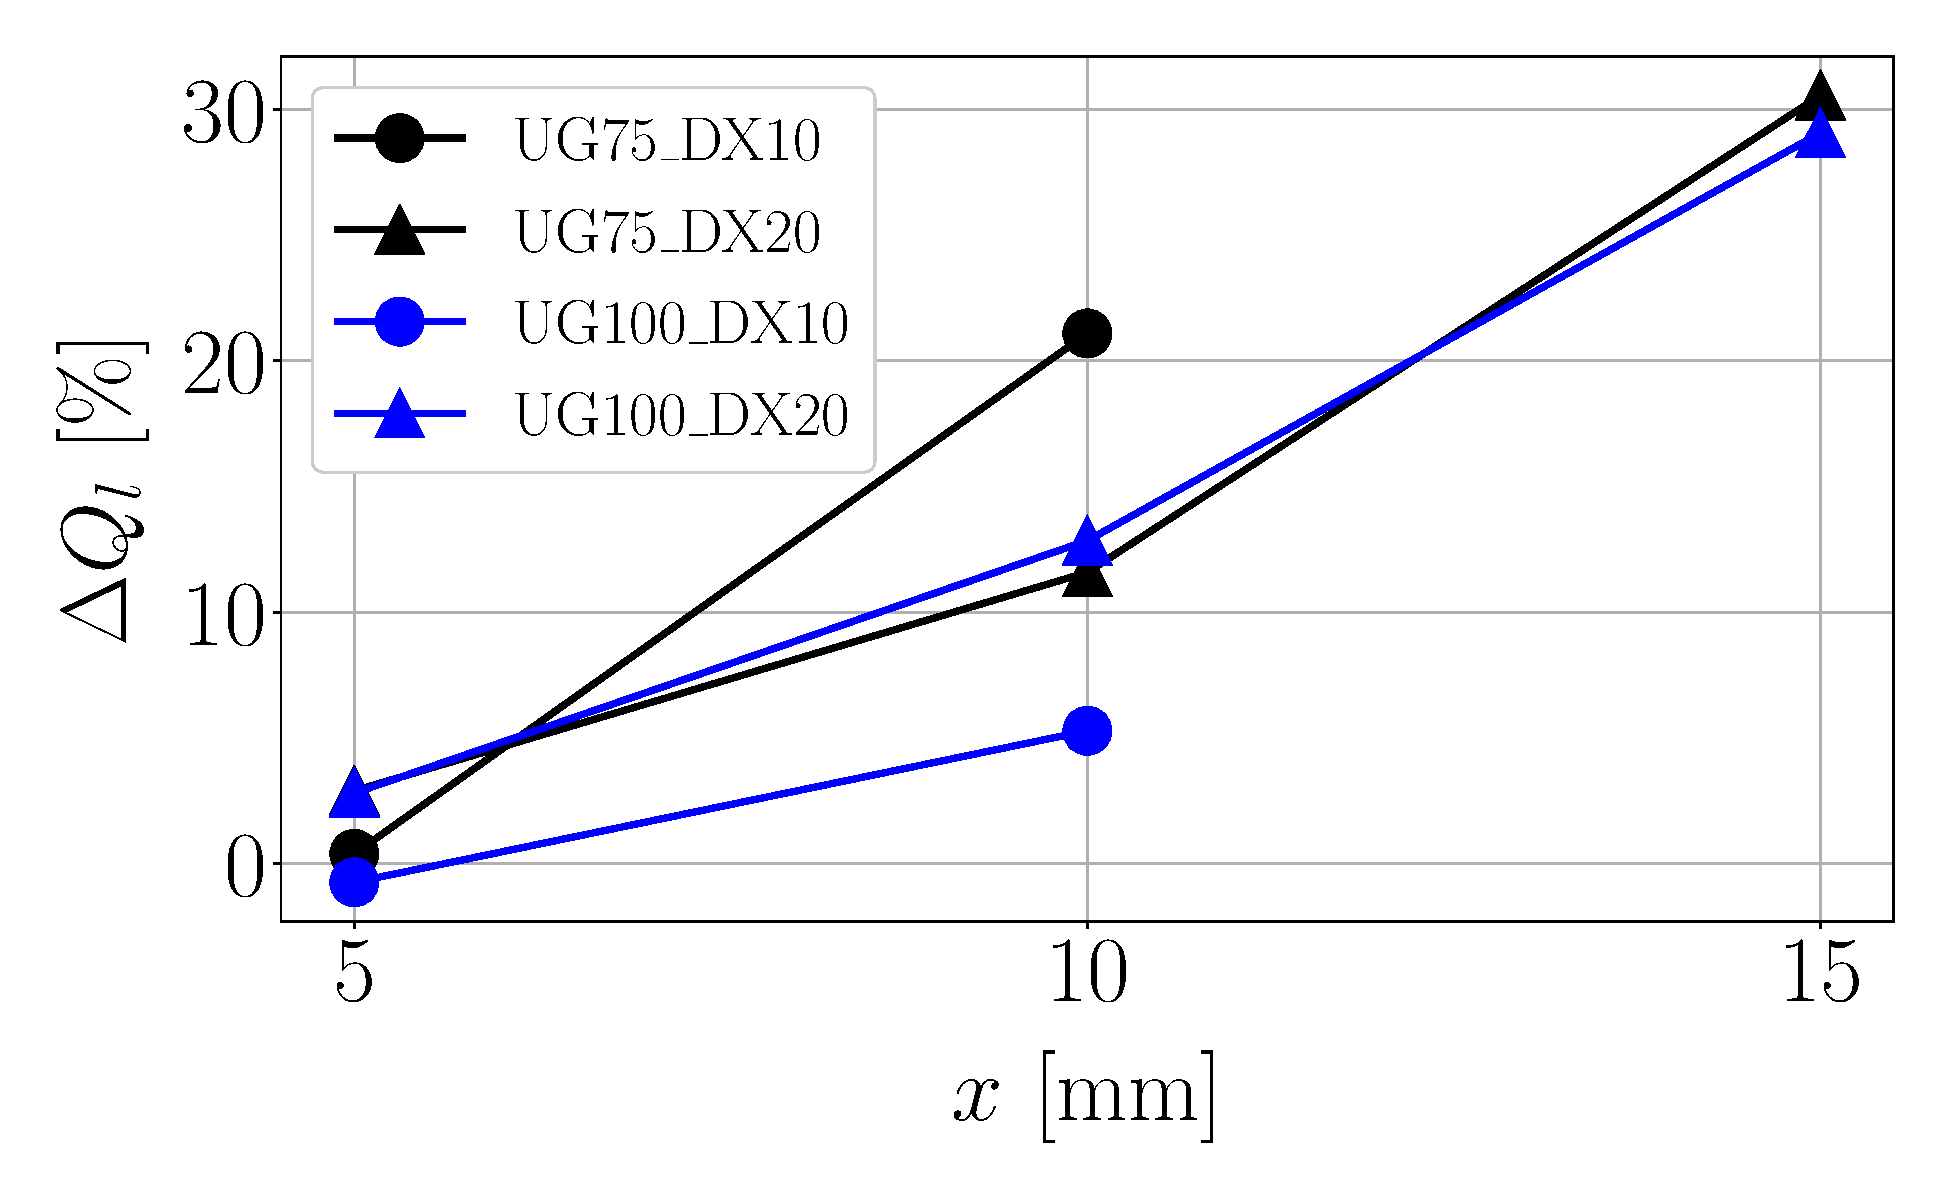
\includegraphics[scale=0.3]{./part2_developments/figures_ch5_resolved_JICF/flow_rates_ibs/Ql_loss_with_x}
   \vspace*{-0.2in}
   \caption{Relative loss of total liquid flow rates loss $\Delta Q_l$ with axial distance.}
   \label{fig:delta_Ql_with_x}
\end{figure}

Finally, the flow rates obtained for all IBs have been discretized at each timestep and averaged, yielding the spatial maps of Figure \ref{fig:ibs_spatial_distributions}. Each IB has been discretized into squared probes of 1 mm sides, and then the flow rates through each probe have been divided by the probe's surface to give the volume flux $q_l$ according to Eq. (\ref{eq:ch4_volume_flux_definition}). The flux maps display in all cases a circular distribution of flux of the IBs since there is more liquid concentration in the center part of the spray than at its edges, as also observed in experimental studies \citemColor[wu_spray_1998,becker_breakup_2002].  The spray boundaries become wider in the lateral ($y$) and vertical ($z$) directions downstream the injection location due to the spray opening with axial distance. Larger values of maximum $q_l$ are found closer to the jet: this is due to a higher liquid concentration closer to the injector since the spray is less disperse in the lateral and vertical directions, which combined with larger mean fluxes (see Figure \ref{fig:IB_bargraph}) results in larger values of $q_l$. 



\clearpage

\begin{figure}[ht]
\flushleft
\begin{subfigure}[b]{1.1\textwidth}
	\flushleft
   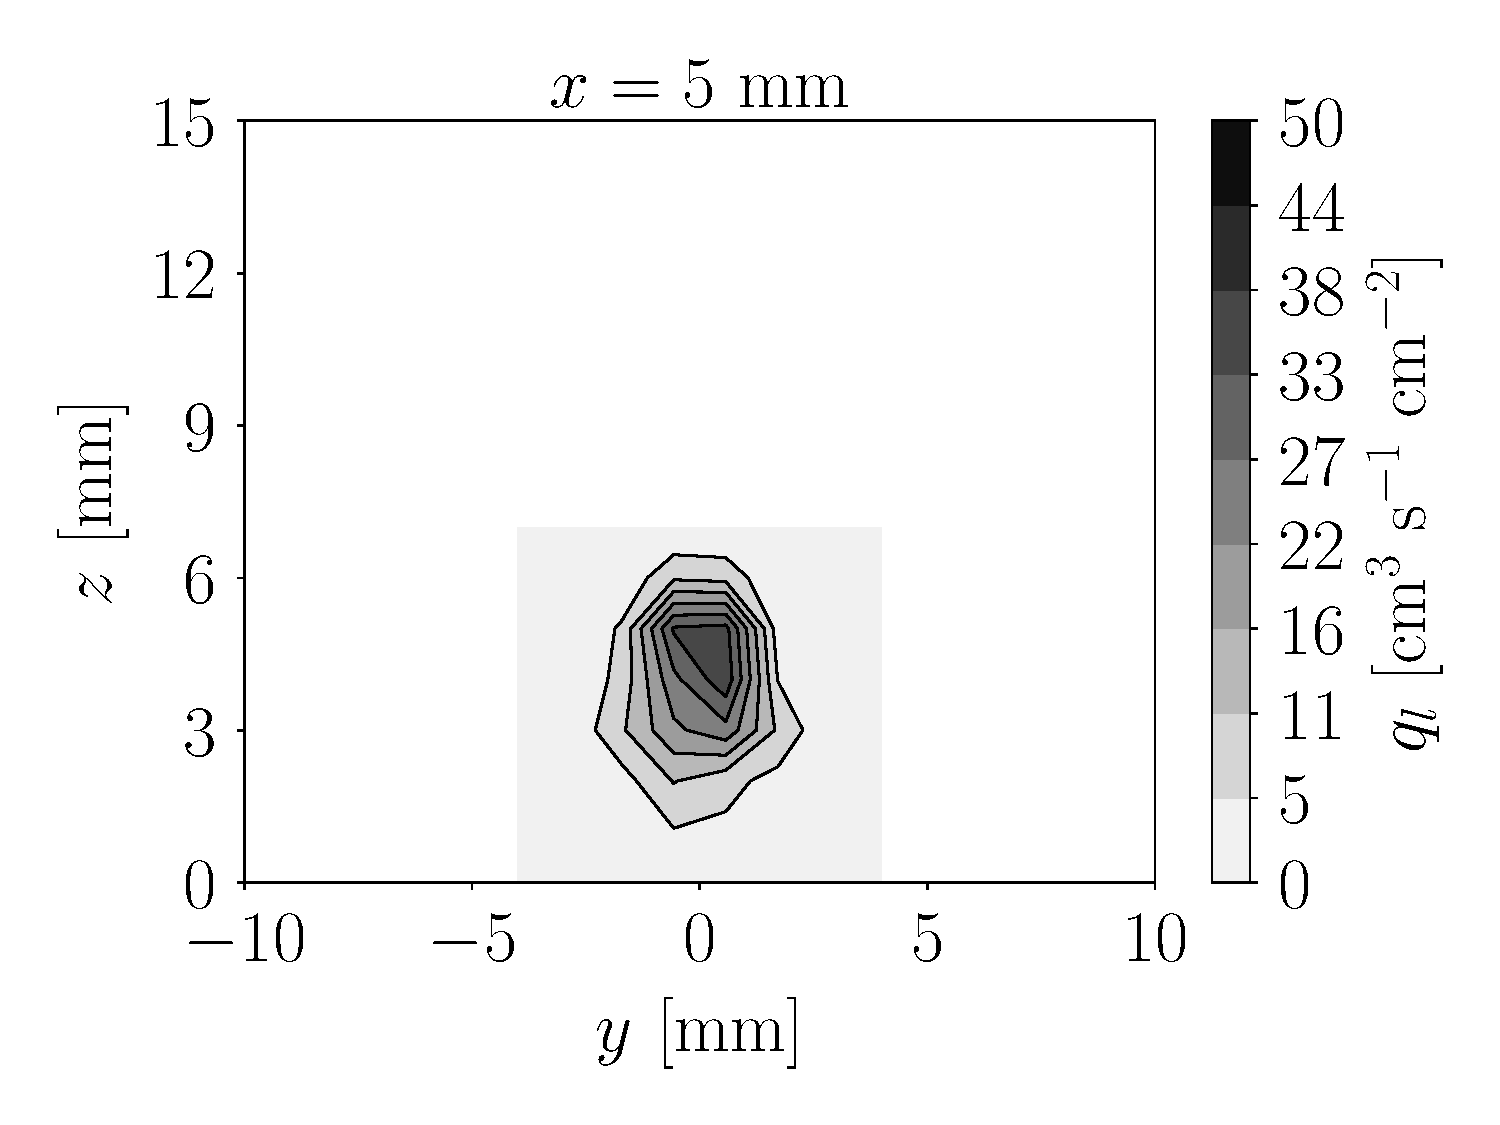
\includegraphics[scale=0.225]{./part2_developments/figures_ch5_resolved_JICF/flow_rates_ibs/spatial_maps/UG75_DX10_x05mm_volume_flux}
   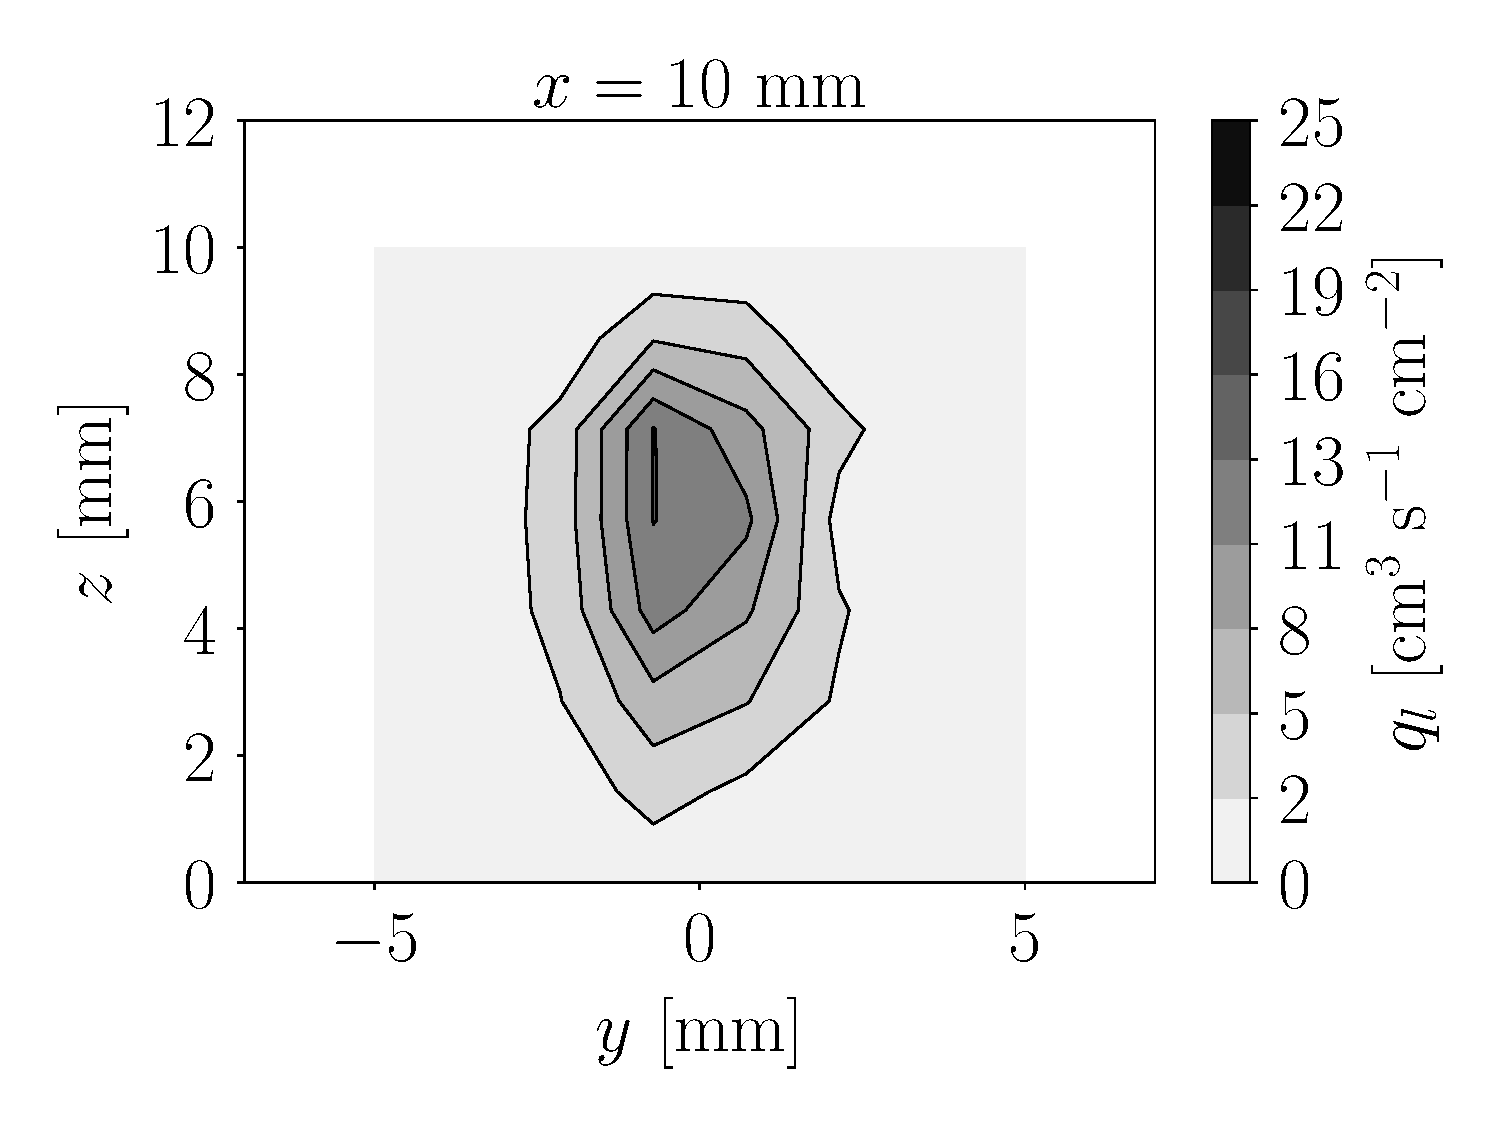
\includegraphics[scale=0.225]{./part2_developments/figures_ch5_resolved_JICF/flow_rates_ibs/spatial_maps/UG75_DX10_x10mm_volume_flux}
   \vspace*{-0.1in}
	\caption{Case UG75\_DX10}
\end{subfigure}


\vskip\baselineskip


\begin{subfigure}[b]{1.1\textwidth}
	\flushleft
   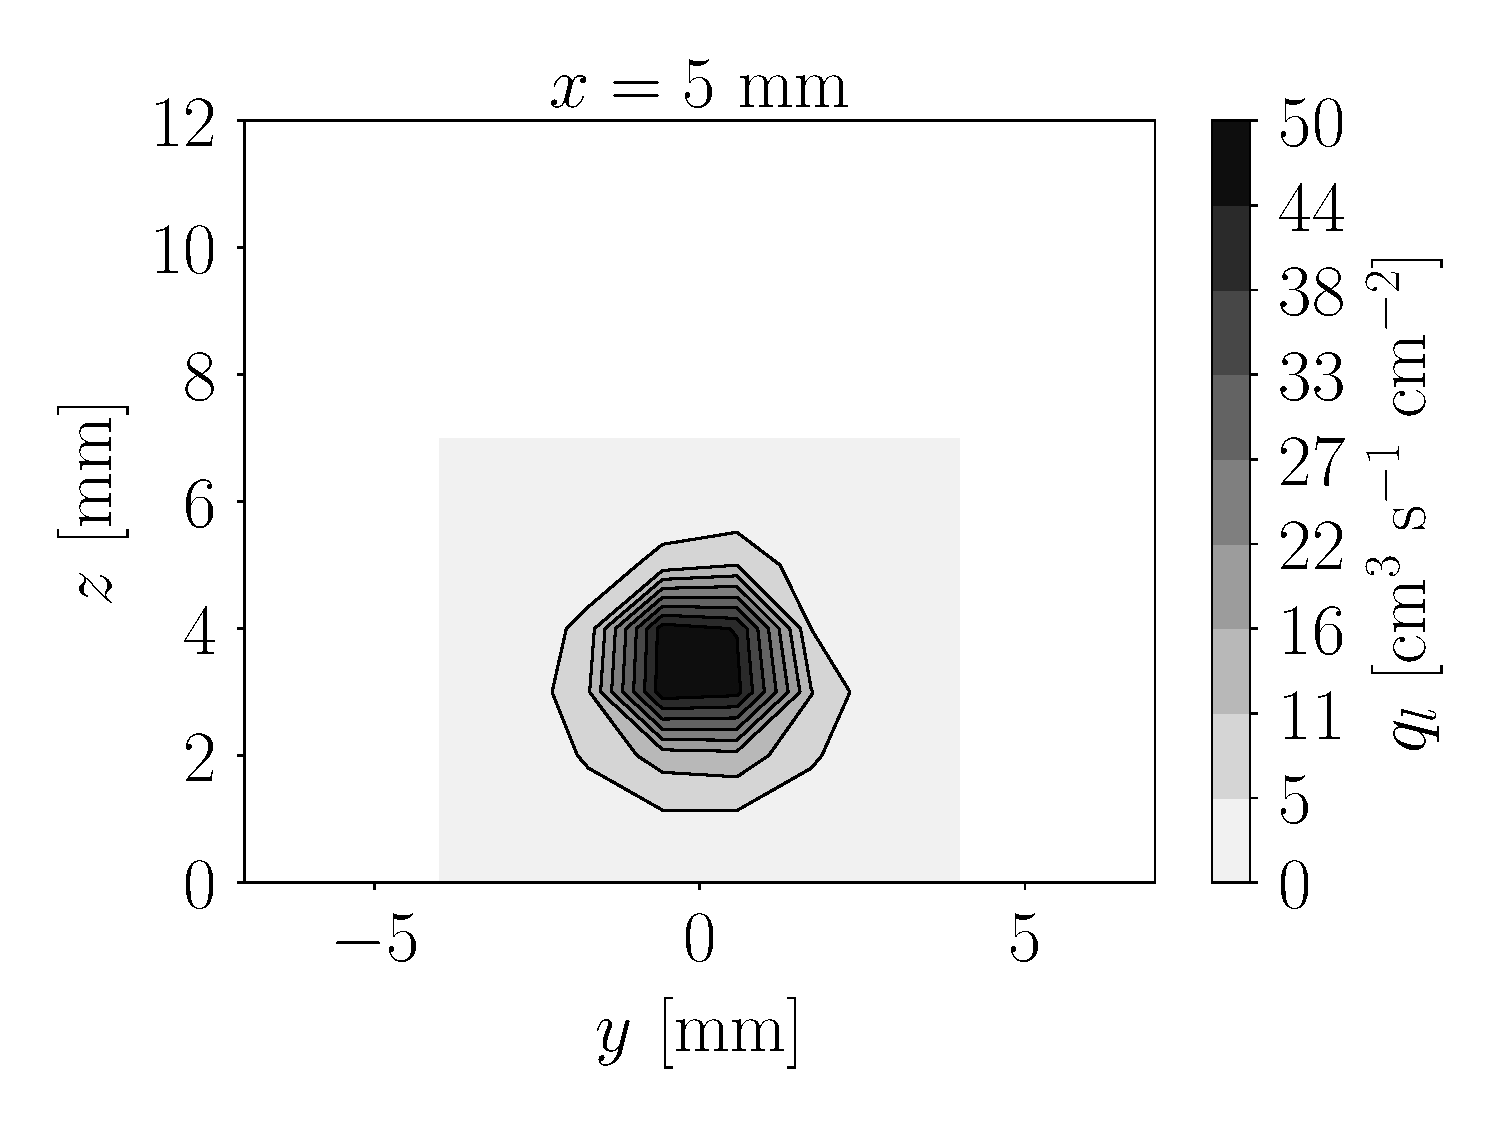
\includegraphics[scale=0.225]{./part2_developments/figures_ch5_resolved_JICF/flow_rates_ibs/spatial_maps/UG75_DX20_x05mm_volume_flux}
   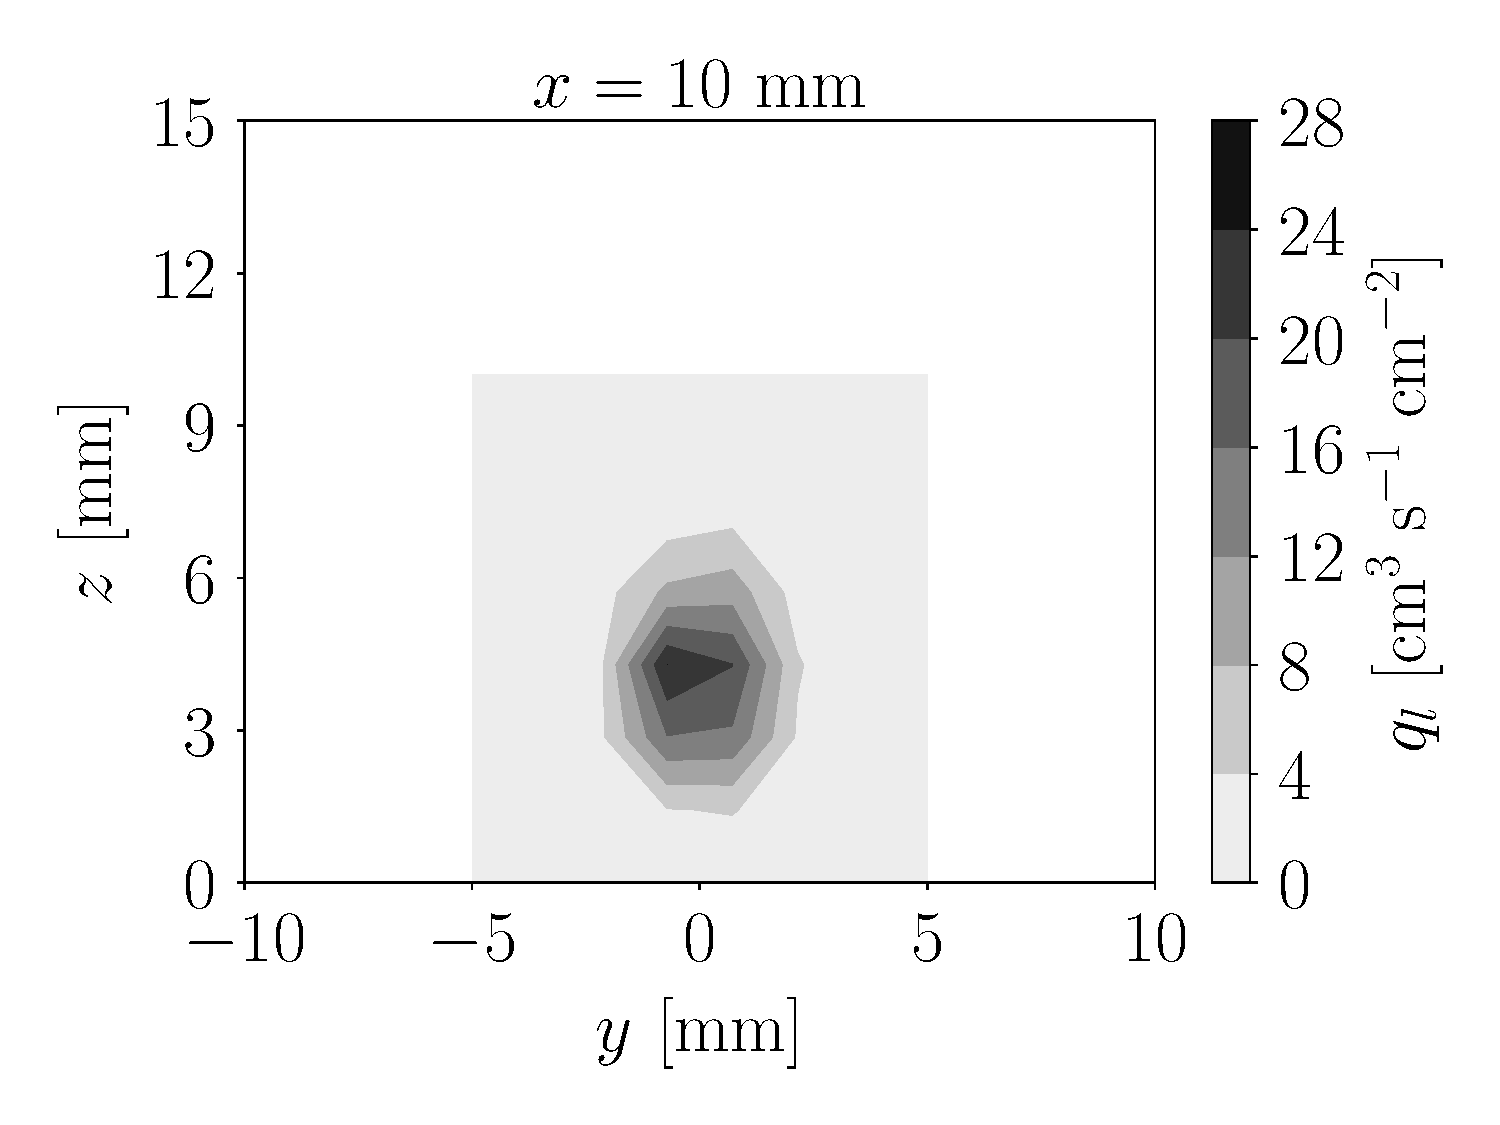
\includegraphics[scale=0.225]{./part2_developments/figures_ch5_resolved_JICF/flow_rates_ibs/spatial_maps/UG75_DX20_x10mm_volume_flux}
   \includegraphics[scale=0.225]{./part2_developments/figures_ch5_resolved_JICF/flow_rates_ibs/spatial_maps/UG75_DX20_x15mm_volume_flux}
   \vspace*{-0.1in}
	\caption{Case UG75\_DX20}
\end{subfigure}

\vskip\baselineskip

\begin{subfigure}[b]{1.1\textwidth}
	\flushleft
   \includegraphics[scale=0.225]{./part2_developments/figures_ch5_resolved_JICF/flow_rates_ibs/spatial_maps/UG100_DX10_x05mm_volume_flux}
   \includegraphics[scale=0.225]{./part2_developments/figures_ch5_resolved_JICF/flow_rates_ibs/spatial_maps/UG100_DX10_x10mm_volume_flux}
   \vspace*{-0.1in}
	\caption{Case UG100\_DX10}
\end{subfigure}

\vskip\baselineskip

\begin{subfigure}[b]{1.1\textwidth}
	\flushleft
   \includegraphics[scale=0.225]{./part2_developments/figures_ch5_resolved_JICF/flow_rates_ibs/spatial_maps/UG100_DX20_x05mm_volume_flux}
   \includegraphics[scale=0.225]{./part2_developments/figures_ch5_resolved_JICF/flow_rates_ibs/spatial_maps/UG100_DX20_x10mm_volume_flux}
   \includegraphics[scale=0.225]{./part2_developments/figures_ch5_resolved_JICF/flow_rates_ibs/spatial_maps/UG100_DX20_x15mm_volume_flux}
   \vspace*{-0.1in}
	\caption{Case UG100\_DX20}
\end{subfigure}

   \caption{Spatial distributions of volume fluxes obtained from interior boundaries}
\label{fig:ibs_spatial_distributions}
\end{figure}

\clearpage

\subsection{Computational performances and costs}
\label{subsec:ch5_computational_performances}

Table \ref{tab:jicf_Ncores_Ncells_Ndrops} shows the numbers of cores, cells and droplets present at $t^* = 12$. At this instant all jets are developed but liquid has not reached yet the sponge layer (i.e. the axial location where it is artificially removed), hence allowing for a comparison among cases. The number of cores evolves in each run as the number of cells increase due to AMR for keeping a ratio $N_\mathrm{cells} / N_\mathrm{cores}$ between 100,000 and 150,000, which is optimum for parallellization purposes \citepColor[trobec_introduction_2018]. As observed, changing the interface resolution $\Delta x_\mathrm{min}$ for a given operating point multiplies the number of droplets by 6. A larger quantity of droplets with a finer interface cell size increases substantially the number of elements, of the order of 5 times. Then, the number of cores rises by the same factor in order to keep the ration $N_\mathrm{cores}/N_\mathrm{cells}$ within the optimal range for paralellization. A comparison of operating conditions for the fine mesh resolution shows that the number of droplets and cells are larger for the high Weber number than for the low one, which is coherent since the velocities are larger in the former one and more droplets are expected to be formed by surface breakup. %When looking at the same mesh resolution, however, it is seen that the number of droplets stays generated is the same: this might be due to the surface breakup phenomenon not being sufficiently resolved for these cases. Also, by comparing the cases with and without turbulence (for the high Weber, coarse resolution), it is observed that the case without turbulence contains less droplets and less elements than when turbulence is injected. Therefore, that the addition of synthetic turbulence enhances breakup and produces more droplets. This was also reflected in Table \ref{tab:jicf_SLI_Ndr_accumulated}, which shows that more droplets have been accumulated in the case with turbulence for accumulation time. Further investigating the effect of synthetic turbulence on the quantity of droplets produced through atomization would require to perform a simulation with a fine resolution $\Delta x_\mathrm{min} = 10$, where atomization is better resolved, without turbulence. This has not been done here due to the high cost of the fine simulations and since the study of turbulence injection is not the main purpose of this work.

\begin{table}[!h]
\centering
\caption{Computational cores, mesh cells and total number of droplets present at the domain for JICF simulations at $t^* = 12$}
\begin{tabular}{cccc}
\thickhline
\textbf{Case} &  $N_\mathrm{cores}$ & $N_\mathrm{cells}$ ($\cdot 10^6$) & $N_\mathrm{drops}$\\
\thickhline 
UG75\_DX10 & 3840  & 430 & 2221 \\ 
UG75\_DX20 & 768 & 100 & 394 \\
UG100\_DX10 & 4224 & 440 & 2563 \\ % restart_03.o, iter 835
UG100\_DX20 & 768 & 104 & 393 \\ % restart_01.o, iter 1990
UG100\_DX20\_NT & 768 & 92 & 326 \\ % restart_01.o,  iter 1720
\thickhline
\end{tabular}
\label{tab:jicf_Ncores_Ncells_Ndrops}
\end{table}



To assess the computational performances of the performed simulations, a Reduced Computational Time (RCT) can be defined as \citepColor[janodet_massively_2022]:

\begin{equation}
\label{eq:RCT_definition}
\mathrm{RCT} = \frac{\mathrm{WCT} ~ N_\mathrm{cores}}{N_\mathrm{iter}~N_\mathrm{cv}}
\end{equation}

where WCT is the Wall Clock Time, $N_\mathrm{cores}$ the number of cores used by the computations, $N_\mathrm{iter}$ the number of temporal iterations performed, and $N_\mathrm{cv}$ the total number of node-based control volumes in the computational domain. RCT, which is expressed in time units, can therefore be used to compare the cost of the different simulations performed independently of the number of cores, iterations and elements they use. The RCT is calculated for each computational routine of the numerical methodology ACLS/AMR, then the different RCTs are added to yield the total RCT of the simulations. These contributions are:

\begin{equation}
\label{eq:RCT_contributions}
\mathrm{RCT} = \mathrm{RCT}_\mathrm{ACLS} + \mathrm{RCT}_\mathrm{AMR} + \mathrm{RCT}_\mathrm{NS}
\end{equation}

Where the subindex ACLS indicates the contribution of the ACLS methodology without mesh refinement ($\S$\ref{subsec:ch2_ACLS}), AMR indicates the contribution of the mesh refinement ($\S$\ref{subsec:ch2_ACLS}), and $\mathrm{RCT}_\mathrm{NS}$ denotes the contribution of the routines devoted to resolution of the Navier-Stokes equation, which in YALES2 employ a linear solver to compute the Poisson equation \citepColor[moureau_design_2011].

Additionally, the CPU time can be computed as follows:

\begin{equation}
\label{eq:t_CPU_definition}
t_\mathrm{CPU} = \mathrm{WCT} ~ N_\mathrm{cores}
\end{equation}

which expresses the computational cost in hours of a simulation. Table \ref{tab:jicf_computational_performances} reports the RCT values and the ratio $t_\mathrm{CPU} / t^*$. In all simulations, the fastest routine is the NS while the slowest one, and therefore the most expensive, is AMR. For cases UG75\_DX20 and UG100\_DX20, the reduced time spent in the routines ACLS, AMR and NS is similar. Comparing cases with and without turbulence injection shows that there is a reduction of the RCT in the AMR for the latter case due to a lower degree of atomization which produces less droplets (see Table \ref{tab:jicf_Ncores_Ncells_Ndrops}) and, therefore, less surface of liquid interface to remesh. The largest differences are found among resolutions: in the fine cases, all the RCT contributions increase from 2 to 3 times with respect to their homologues from the coarse simulations. This increase is mainly due to AMR, which is therefore the most time-consuming and computationally expensive routine. 

\clearpage



\begin{table}[!ht]
\centering
\caption{Computational performances from JICF simulations at $t^* = 12$}
\begin{tabular}{cccccc}
\thickhline
\textbf{Case} &  $\mathrm{RCT}~[\mu \mathrm{s}]$ & $\mathrm{RCT}_\mathrm{ACLS}~[\mu \mathrm{s}]$ & $\mathrm{RCT}_\mathrm{AMR}~[\mu \mathrm{s}]$ & $\mathrm{RCT}_\mathrm{NS}~[\mu \mathrm{s}]$ & $t_\mathrm{CPU} / t^*  ~ [\mathrm{h}]$\\
\thickhline 
UG75\_DX10 & 1549.7 & 192.0 & 1182.6 & 175.1 &  5252 \\ % t_cpu/t_phys: 204,200
UG75\_DX20 & 494.1 & 88.8 & 362.3 & 43.0 &  440 \\ % t_cpu/t_phys: 17,100
UG100\_DX10 & 1643.6 & 162.5 & 1369 & 112.1&  5580 \\ % t_cpu/t_phys: 277,800
UG100\_DX20 & 517.5 & 105.8 & 361.1 & 50.6 & 414  \\ % t_cpu/t_phys: 21,500
UG100\_DX20\_NT & 444.0 & 105.0 & 295.0 & 44.0 & 342  \\ % t_cpu/t_phys: 17,700
\thickhline
\end{tabular}
\label{tab:jicf_computational_performances}
\end{table}

Figure \ref{fig:SLI_cost_convergence_all} reports the computational cost in CPU hours ($t_\mathrm{CPU}$) and the ratio between CPU hours and physical time simulated ($t_\mathrm{CPU}/t_\mathrm{ph}$). As expected, more CPU hours are devoted to the fine simulations, both in absolute value and per milisecond simulated. Reducing the interface cell size by two increases the cost by a larger extent through two contributions: 

\begin{itemize}

	\item Lower timesteps $\Delta t$ in the fine simulations due to smaller cell sizes. The latter is estimated from the CFL number (which is equal in all simulations) according to the following expression:

\begin{equation}
\label{eq:ch5_dt_CFL}
\Delta t \leq \min \left( \frac{\mathrm{CFL} ~   \Delta x }{|\textbf{u}|} \right)
\end{equation}

	\item A larger number of cells in the fine simulations due to more droplets being resolved.

\end{itemize}

Figure \ref{fig:SLI_cost_convergence_all} also shows that high Weber simulations are more expensive than the low Weber one. The reasons are the two same ones as aforementioned. The higher Weber cases have larger velocities, which for identical resolution yield lower timesteps according to Eq. (\ref{eq:ch5_dt_CFL}). Then, these simulations also contain a larger amount of droplets due to higher shear, which in turn increase the number of cells with respect to the low Weber computations.


\begin{figure}[ht]
	\centering
   \includegraphics[scale=0.225]{./part2_developments/figures_ch5_resolved_JICF/SLI_cost_for_convergence/cost_all_simulations}
   \caption{Cost of the JICF simulations in CPU time and CPU per physical times simulated}
   \label{fig:SLI_cost_convergence_all}
\end{figure}




From these analyses, it can be concluded that  augmenting the resolution twice will increase the cost of the simulations by a larger factor, and that most of the computational resources are devoted to AMR. Nevertheless, it is thanks to the AMR methodology that such computations become possible. Performing resolved simulations with such fine resolutions in unstructured grids would be unfeasible if the interface cell size $\Delta x_\mathrm{min}$ had to be specified in all the domain.



\clearpage

\section{SLI building}
\label{sec:ch5_SLI_building}

This section reports the results from post-processing data from the resolved simulations for creating a Smart Lagrangian Injector (SLI). Firstly, the dense core topology and momentum parameters to obtain its net force are provided. Next, the spray sampled through lagrangian tracking is postprocessed and spatially discretized. The process sprays will serve as boundary conditions for the liquid phase in dispersed-phase simulations.



\subsection{Dense core characterization for ALM}
\label{subsec:ch5_DC_topology_characterization}



%A relevant characteristic of liquid jets is the dense core (DC) region, which is the coherent liquid volume close to the injection nozzle where atomization starts to take place. The DC is an important feature of primary atomization, and is dependent on the injection nozzle and the operating conditions. In the case of a JICF such as the one studied in this thesis, it can be obtained as the liquid structure containing the largest liquid volume of all the present structures. The DC undergoes instabilities that are presented as Kelvin-Helmholtz or Rayleight-Taylor processes that will cause column breakup. Simultaneously, droplets are being shed along the sides of the DC due to surface breakup. These phenomena are particular of the jet in crossflow and are not present as such in other atomizer configurations. %Nevertheless, other configurations will present their own DC structures and breakup morphologies \citepColor[rezayat_high-speed_2021].

The dense core (DC) of a JICF is the focus of numerous studies, since it creates an important blockage effect in the incoming air that propagates turbulent structures further downstream, affecting atomization and spray dispersion. Pioneer JICF experimental studies \citepColor[wu_breakup_1997] focused on obtaining the \textbf{breakup point} of the DC by studying side shadowgraphs from the JICF. More recent works \citepColor[patil_liquid_2021] tried also to determine its width and its lateral opening angle. Nevertheless, experimental and numerical studies of the DC topology in JICF are scarce nowadays, specially at operating conditions where surface breakup predominates (since the visualization of the jet is hindered by a large number of small droplets generated).

In this work, the DC topology is determined and studied from the resolved atomization simulations in order to provide input parameters to the Actuator Line Method (ALM) for modeling the gaseous field disturbances in dispersed-phase computations. The procedure followed to process the DC topology is detailed in Appendix \ref{app:processing_JICF_DC_breakup_point}, while here only results are presented. \\


%The methodologies proposed to process the DC topology and to estimate its net force are explained next, followed then by the results obtained from the simulations.

In first place, the time evolution of the breakup point coordinates and width are shown in Figure \ref{fig:JICF_xb_zb_w_evolution}. Time has been non-dimensionalized according to Eq. (\ref{eq:t_prime_with_tau_drx10}). All signals display a sawtooth shape that reflects the dynamic behaviour of the dense core: increasing values correspond to ligaments being formed from the dense core (i.e. the breakup point $x_\mathrm{b}, z_\mathrm{b}$ moves further downstream and upwards, while the width $w$ increases due to the deformation of the dense core cross-section), then they suffer an abrupt decrease when the ligaments are dettached from the jet, and the process repeats once and again.  This periodic behaviour has been previously observed in several experimental studies  \citepColor[wang_characterization_2011, prakash_liquid_2018].

%Each steep decay in the sawtooth signals $x_b (t), z_b (t)$ is associated to a ligament which strips from the liquid column. Therefore, their associated frequencies are of the order of the ligament stripping frequencies. The spectra of signals $x_b (t)$ calculated through FFT are shown in Figure \ref{fig:JICF_DC_FFTs_xb}. The coarse simulations have run for a long physical time and enough sampled points are available in the frequency axis (low $\Delta f$ between consecutive points) to retrieve frequency peaks, while fine simulations have not run long enough and the amount of frequency points is scarce (high $\Delta f$ between consecutive points). Consequently, the frequency peaks present in the fine simulation (located at $f \sim 1~kHz$ for UG100\_DX75 and at $f \sim 2.5~kHz$ for UG100\_DX10) are not accurate enough and might not represent the ligament stripping frequencies, although they give an idea of their order of magnitude. Table \ref{tab:jicf_ligament_shedding_fs_and_tau_str} shows the dominant striping frequencies $f_\mathrm{str}$ in each case and their associated times $\tau_\mathrm{str} = 1/f_\mathrm{str}$. The fine cases show higher breakup frequencies, which are due to a shorter breakup length.



\begin{figure}[ht]
\flushleft
\begin{subfigure}[b]{0.45\textwidth}
	\centering
   \includegraphics[scale=0.25]{./part2_developments/figures_ch5_resolved_JICF/results_dense_core_modeling/instant_xb_zb_w_UG75_DX10}
   \vspace*{-0.3in}
   \caption{Case UG75\_DX10}
   \label{fig:instant_xb_zb_w_UG75_DX10} 
\end{subfigure}
\hfill
\begin{subfigure}[b]{0.45\textwidth}
	\centering
   \includegraphics[scale=0.25]{./part2_developments/figures_ch5_resolved_JICF/results_dense_core_modeling/instant_xb_zb_w_UG75_DX20}
   \vspace*{-0.3in}
   \caption{Case UG75\_DX20}
   \label{fig:instant_xb_zb_w_UG75_DX20}
\end{subfigure}

\vskip\baselineskip
\vspace*{-0.1in}

\begin{subfigure}[b]{0.45\textwidth}
	\centering
   \includegraphics[scale=0.25]{./part2_developments/figures_ch5_resolved_JICF/results_dense_core_modeling/instant_xb_zb_w_UG100_DX10}
   \vspace*{-0.30in}
   \caption{Case UG100\_DX10}
   \label{fig:instant_xb_zb_w_UG100_DX10} 
\end{subfigure}
\hfill
\begin{subfigure}[b]{0.45\textwidth}
	\centering
   \includegraphics[scale=0.25]{./part2_developments/figures_ch5_resolved_JICF/results_dense_core_modeling/instant_xb_zb_w_UG100_DX20}
   \vspace*{-0.30in}
   \caption{Case UG100\_DX20}
   \label{fig:instant_xb_zb_w_UG100_DX20}
\end{subfigure}
   \caption{Variation with time of the dense core breakup point coordinates $x_\mathrm{b}, z_\mathrm{b}$ and width $w$.}

\label{fig:JICF_xb_zb_w_evolution}
\end{figure}


%\begin{figure}[ht]
%\flushleft
%\begin{subfigure}[b]{0.45\textwidth}
%	\centering
%   \includegraphics[scale=0.25]{./part2_developments/figures_ch5_resolved_JICF/results_dense_core_modeling/FFTs_UG75}
%   \vspace*{-0.25in}
%   \caption{Low Weber cases}
%   \label{fig:JICF_DC_FFT_UG75} 
%\end{subfigure}
%\hspace{0.2in}
%\begin{subfigure}[b]{0.45\textwidth}
%	\centering
%   \includegraphics[scale=0.25]{./part2_developments/figures_ch5_resolved_JICF/results_dense_core_modeling/FFTs_UG100}
%   \vspace*{-0.25in}
%   \caption{High Weber cases}
%   \label{fig:JICF_DC_FFT_UG100}
%\end{subfigure}
%   \caption{Spectra of $x_b$ signals}
%\label{fig:JICF_DC_FFTs_xb}
%\end{figure}
%
%\begin{table}[!h]
%\centering
%\caption{Dominant frequencies and associated timescales of spectra from Figure \ref{fig:JICF_DC_FFTs_xb}}
%\begin{tabular}{cccccc}
%\thickhline
%\textbf{Case} &  UG75\_DX10 & UG75\_DX20 & UG100\_DX10 & UG100\_DX20 &  UG100\_DX20\_NT \\
%\hline
%$f_\mathrm{str}~[kHz]$ & 1.60 & 0.72 & 2.37 & 0.53 & 1.34 \\
%$\tau_\mathrm{str}~[\mu s]$ & 625 & 1389 & 422 & 1887 & 746 \\
%\thickhline
%\end{tabular}
%\label{tab:jicf_ligament_shedding_fs_and_tau_str}
%\end{table}


To define an actuator representing the dense core in dispersed phase simulations, the mean values of the breakup point coordinates and width will be used. Hence, the mean value of the signals from Figure \ref{fig:JICF_xb_zb_w_evolution} are calculated. The evolution of the mean values with time (i.e. convergence with time) is shown in Figure \ref{fig:dense_core_mean_parameters_convergence}. As observed, the simulations performed with the coarse interface cell size $\Delta x_\mathrm{min} = 20~\mu m$ are converged for the three parameters $x_\mathrm{b}, z_\mathrm{b}$ and $w$ (except for $z_\mathrm{b}$ in case UG75\_DX20, as this parameter seems the one taking longer time to achieve convergence). The fine resolutions $\Delta x_\mathrm{min} = 10~\mu m$ have not yet achieved full convergence. 

\begin{figure}[ht]
\flushleft
\begin{subfigure}[b]{0.3\textwidth}
	\flushleft
   \includegraphics[scale=0.225]{./part2_developments/figures_ch5_resolved_JICF/results_dense_core_modeling/convergence_mean_xb}
\end{subfigure}
\hfill
\begin{subfigure}[b]{0.3\textwidth}
	\flushleft
   \includegraphics[scale=0.225]{./part2_developments/figures_ch5_resolved_JICF/results_dense_core_modeling/convergence_mean_zb}
\end{subfigure}
\hfill
\begin{subfigure}[b]{0.3\textwidth}
	\flushleft
   \includegraphics[scale=0.225]{./part2_developments/figures_ch5_resolved_JICF/results_dense_core_modeling/convergence_mean_width}
\end{subfigure}
	\vspace*{-0.2in}
   \caption{Evolution of mean geometric parameters of the dense core}
\label{fig:dense_core_mean_parameters_convergence}
\end{figure}

The final mean values obtained for the geometrical parameters are shown in Figure \ref{fig:dense_core_mean_parameters_scatterplots}. The bars in the figures denote the standard deviation of the instantaneous signals. Figure \ref{fig:dense_core_mean_parameters_scatterplots}a shows that the mean values for the coarse resolution are below the $\overline{z_\mathrm{b}} = \overline{x_\mathrm{b}}$, indicating that the dense core penetrates further along the streamwise direction $x$ than in the vertical $z$. On the contrary, the points for the fine resolution are located above this line, which shows that the dense core is elongated along the vertical direction. This graph also show iso-lines of the dense core length $L_\mathrm{DC}$. Lengths are similar for identical resolutions regardless the operating condition, but present significant differences among resolutions. Fine simulations present a shorter dense core than the coarse ones; in other words, fine simulations capture an earlier breakup than the coarse ones. This is due to the resolution of instabilities in the fine resolution, which foster an earlier breakup of the liquid dense core \citemColor[xiao_les_2014,prakash_liquid_2018,crialesi-esposito_analysis_2019].

\begin{figure}[ht]
\flushleft
\begin{subfigure}[b]{0.45\textwidth}
	\centering
   \includegraphics[scale=0.25]{./part2_developments/figures_ch5_resolved_JICF/results_dense_core_modeling/map_xb_zb}
   \label{fig:dense_core_mean_parameters_scatterplots_zb_xb}
\end{subfigure}
%\hfill
\hspace{0.25in}
\begin{subfigure}[b]{0.45\textwidth}
	\centering
   \includegraphics[scale=0.25]{./part2_developments/figures_ch5_resolved_JICF/results_dense_core_modeling/map_xb_width}
   \label{fig:dense_core_mean_parameters_scatterplots_w_xb}
\end{subfigure}
   \vspace*{-0.30in}
\caption{Mean values for the dense core geometric parameters}
\label{fig:dense_core_mean_parameters_scatterplots}
\end{figure}

Figure \ref{fig:dense_core_mean_parameters_scatterplots} reveals also a slight dependendency of the mean parameters with respect to the operating conditions. For the coarse simulations, the breakup coordinates $\overline{x_\mathrm{b}}$ ($\overline{z_\mathrm{b}}$) are slightly lower (higher) for the low $We$ operating point: increasing aerodynamic gas forces pushes the breakup point further downstream and upwards. This is coherent with the experimental results from \citeColor[patil_liquid_2021], who obtained a correlation for the axial breakup point which varies with the gas Weber number as $x_\mathrm{b} \propto We_g^{0.1}$. The dependency with $We_g$ is however very weak, as also found in Figure \ref{fig:dense_core_mean_parameters_scatterplots}a since the changes in mean values are not actually very significant. This experimental study also includes a correlation for the width $w$ which depends solely on the $q$ factor, also coherent with the results from Figure \ref{fig:dense_core_mean_parameters_scatterplots}b for the coarse resolution. It is to bear in mind that these experiments do not correspond to the operating points studied here, thus the actual dependencies and their intensities (i.e. exponent constants from the correlations) might be different at these conditions. The present computational study shows, however, similar qualitative trends. 

\clearpage

%The fine resolution shows a dependency of $w$ with the operating point: however, it is to bear in mind that the parameters from the fine resolutions are not fully converged, and therefore definitive conclusions cannot be extracted from these results. Further analysis would require running longer the fine simulations to reach convergence of the parameters. 


%\begin{table}[!h]
%\centering
%\caption{Dense core mean lengths $L_\mathrm{DC}$ and widths $w$ from JICF simulations performed}
%\begin{tabular}{cccccc}
%\thickhline
%\textbf{Case} &  UG75\_DX10 & UG75\_DX20 & UG100\_DX10 & UG100\_DX20 &  UG100\_DX20\_NT \\
%\hline
%$L_\mathrm{DC}/d_\mathrm{inj}$ & 9.05 & 12.47 & 8.75 & 12.53 & 12.49 \\
%$w/d_\mathrm{inj}$ & 4.60 & 4.29 & 4.62 & 4.28 & 4.24 \\
%\thickhline
%\end{tabular}
%\label{tab:jicf_L_DC_values}
%\end{table}

Table \ref{tab:dense_core_geometry_pressures_and_force_parameters} shows a summary of all the relevant parameters for characterizing the dense core topology and its net force (momentum) in all simulations. These values are taken as input parameters to the ALM model for the dispersed-phase simulations of Chapter \ref{ch6:jicf_lgs_simulations}.


\begin{table}[!h]
\centering
\caption{Dense core characterization: geometric and momentum parameters}
\vspace*{-0.1in}
\begin{tabular}{ccccccc}
\thickhline
\textbf{Case} & $L_\mathrm{DC}/d_\mathrm{inj}$ & $w/d_\mathrm{inj}$ & $S_\mathrm{DC}$ [mm$^2$] & $p_\mathrm{windward}$ [Pa] & $p_\mathrm{leeward}$ [Pa]  & $|\boldsymbol{F}_\mathrm{DC}|$ [N] \\
\thickhline 
UG75\_DX10  & 9.05 & 4.60 & 5.1 & 5,200 & -6,100 & 0.058  \\
UG75\_DX20  & 12.47 & 4.29 & 6.7 & 3,200 & -8,000 &  0.074 \\
UG100\_DX10 & 8.75 & 4.62 & 5.0 & 10,400 & -8,800 & 0.095 \\
UG100\_DX20 & 12.53 & 4.28 & 6.7 & 5,700 & -14,000 & 0.13 \\
UG100\_DX20\_NT & 12.49 & 4.24 & 6.6 & 5,000 & -14,000 & 0.12 \\
\thickhline
\end{tabular}
\label{tab:dense_core_geometry_pressures_and_force_parameters}
\end{table}




\vspace*{-0.05in}

\subsection{Spray characterization}
\label{subsec:ch5_sec_spray_characterization}

%\subsubsection{Sampling procedure for droplets}

This section presents a characterization of the global spray sampled from the resolved simulations through lagrangian tracking of the liquid structures as described in $\S$\ref{subsec:SLI_spray_sampling}. The sampling planes perpendicular to crossflow are those shown in Figure \ref{fig:jicf_interior_boundaries_surface_measurements}.



\subsubsection*{Establishment of mean sprays}

Droplets are sampled and accumulated with time in order to get a mean-converged spray. Firstly, an establishment time of $t^{\prime} \sim 2$ for each case is left before droplets start to be accumulated in order to retrieve a representative spray of a established jet. Droplets are then accumulated for a total duration $t_\mathrm{acc}$ reported in Table \ref{tab:jicf_SLI_t_prime_accumulation}. The total physical times simulated $t_\mathrm{ph} \sim t_\mathrm{acc} + 2 \tau_\mathrm{dr_{x=10}}$ are also stated. Both the absolute physical time and the dimensionless time calculated through Eq. (\ref{eq:t_prime_with_tau_drx10}) are shown. From the absolute time, huge differences among coarse and fine simulations can be seen: the former are cheaper and run with a larger timestep than the latter ones, therefore reaching a longer physical time. For the low Weber case, the physical time reached by the coarse simulations goes 10 times beyond the fine ones, while the low Weber case shows a factor of 15 among resolutions. If, on the other hand, the dimensionless times are considered, the ratio of simulated times among resolutions reduce to 8.6 and 12.9 for the low and high Weber cases respectively. This is caused by the differences in the timescale $\tau_\mathrm{dr}$ between resolutions, as these values are lower for the fine simulations (see Table \ref{tab:jicf_characteristic_droplet_sampling_times}). When looking at the convergence of injectors, the timescale $t^{\prime}$ is the one to consider since it relates the droplet arrival time to the sampling planes. On the other hand, when discussing physical characteristic among simulations, it is more convenient to use either the absolute physical time or the dimensionless time defined by the relation to the liquid inertia timescale, Eq. (\ref{eq:t_dimensionless_with_tau_in}).


\begin{table}[!h]
\centering
\caption{Total physical $t_\mathrm{ph}$ and accumulation times $t_\mathrm{acc}$, absolute and dimensionless with Eq. (\ref{eq:t_prime_with_tau_drx10}), for each JICF simulation}
\begin{tabular}{ccccc}
\thickhline
\textbf{Case} & $t_\mathrm{ph}~[\mathrm{ms}]$ &  $t_\mathrm{ph}^{\prime}$ & $t_\mathrm{acc}~[\mathrm{ms}]$  & $t_\mathrm{acc}^{\prime}$  \\
\hline
UG75\_DX10 & 1.08 & 3.64 & 0.53 & 1.79 \\
UG75\_DX20 & 6.30 & 17.70 & 5.48  & 15.40 \\
UG100\_DX10 & 0.78  & 3.58 & 0.37 & 1.67 \\
UG100\_DX20  & 6.16 & 23.84 & 5.57 & 21.54 \\
UG100\_DX20\_NT  & 6.10  & 23.44 & 5.53 &  21.24 \\
\thickhline
\end{tabular}
\label{tab:jicf_SLI_t_prime_accumulation}
\end{table}


The total number of droplets accumulated is shown in Table \ref{tab:jicf_SLI_Ndr_accumulated}. The coarse simulations have sampled more droplets than the fine ones, as they have run for longer physical time. Nevertheless, the number of droplets per milisecond simulated (ratio $N_\mathrm{dr}/t_\mathrm{acc}$) shows that the fine cases generate a larger number of particles, of the order of 5 times more than the coarse simulations. As a consequence, fine simulations need less physical time simulated to produce a converged spray for building lagrangian injectors (more insight is given at the end of $\S$\ref{subsec:ch5_learning_SLI}).

\clearpage


\begin{table}[!h]
\centering
\caption{Number of droplets sampled in JICF simulations: total amount ($N_\mathrm{dr}$) and total amount per accumulation time $N_\mathrm{dr}/t_\mathrm{acc}$}
\begin{tabular}{cccccccc}
\thickhline
\multirow{2}{*}{ \textbf{Case}}  & \multicolumn{3}{c}{$N_\mathrm{dr}$} & & \multicolumn{3}{c}{$N_\mathrm{dr}/t_\mathrm{acc}~[\mathrm{ms}^{-1}]$} \\
\cline{2-4} \cline{6-8}
& $x = 5$ mm & $x = 10$ mm & $x = 15$ mm &  & $x = 5$ mm & $x = 10$ mm & $x = 15$ mm  \\
\thickhline 
UG75\_DX10  & 19384 & 11823 & -  & & 36574 & 22307 & - \\
UG75\_DX20  & 25036 & 20399 & 15979  & & 4569 & 3722 & 2916 \\
UG100\_DX10 & 12832 & 9333 & -  & & 34681 & 25224 & - \\
UG100\_DX20 & 35345 & 29986 & 19885  & & 6346 & 5384 & 3570 \\
UG100\_DX20\_NT & 33443 & 27221 & -  & & 6048 & 4922 & - \\
%UG100\_DX20\_NT & 36443 & 30221 & -  & & 6595 & 5469 & - \\
\thickhline
\end{tabular}
\label{tab:jicf_SLI_Ndr_accumulated}
\end{table}








In first place, the establishment of the accumulated sprays is verified by checking the evolution of SMD and liquid flux $Q_l$, defined respectively by Eqs. (\ref{eq:ch4_SMD_definition}) and (\ref{eq:ch4_Ql_definition}), with time. Figure \ref{fig:ch5_spray_char_establishment} shows the results. As observed, all cases shows stabilization at the end of the sampling period considered. The flow rates show a decrease in the stabilized values with axial distance: the further from the injector, the larger the mass losses, which is coherent with the results obtained from the interior boundaries methodology of $\S$\ref{subsec:ch5_direct_measurement_fluxes_IB}. The SMD values show a decrease of the final values with axial distance, which is expected since the atomization process breaks liquid structures into smaller ones. Further comments on the atomization process are given in the next section. %In both the SMD and $Q_l$ evolutions, abrupt changes in the evolution of the mean quantities are observed for most cases, specially at the beginning of the sampling period. This is due to the fact that, in some instants, large liquid structures generated from the column breakup process will be tracked when crossing the sampling planes: these structures contain a large liquid volume that is reflected in both the SMD and the flux evolution at the same instant. Later on the sampling process, the mean values are more stable and such step changes in the curves are not observed, even though these liquid structures are still being sampled.


\begin{figure}[ht]
	\centering
   \includegraphics[width=0.33\textwidth]{./part2_developments/figures_ch5_resolved_JICF/SPRAY_characterization/establishment_and_fluxes/establishment_UG75_DX10}
   \includegraphics[width=0.33\textwidth]{./part2_developments/figures_ch5_resolved_JICF/SPRAY_characterization/establishment_and_fluxes/establishment_UG75_DX20}
   
	\vskip\baselineskip
	
   \includegraphics[width=0.33\textwidth]{./part2_developments/figures_ch5_resolved_JICF/SPRAY_characterization/establishment_and_fluxes/establishment_UG100_DX10}
   \hspace*{-0.1in}
   \includegraphics[width=0.33\textwidth]{./part2_developments/figures_ch5_resolved_JICF/SPRAY_characterization/establishment_and_fluxes/establishment_UG100_DX20}
   \hspace*{-0.1in}
   \includegraphics[width=0.33\textwidth]{./part2_developments/figures_ch5_resolved_JICF/SPRAY_characterization/establishment_and_fluxes/establishment_UG100_DX20_NT}
   \caption[Establishment of SMD and $Q_l$ in JICF sampling planes]{Establishment of SMD and $Q_l$ in JICF sampling planes. The dashed black line represents the liquid flux injected through the nozzle}
\label{fig:ch5_spray_char_establishment}
\end{figure}


Apart from the SMD and mean flux, the spray is also characterized by its mean and RMS velocity components in the three directions and by the deformation parameters $\alpha, \beta$. The convergence of these parameters is reported in Appendix \ref{app:SLI_convergence}: all these magnitudes show converged values, but are not discussed here. \\



 In order to verify the effectiveness of SLI in terms of liquid mass conservation, the liquid fluxes obtained from lagrangian tracking (i.e. the $Q_l$ values at the last accumulation time instant of Figure \ref{fig:ch5_spray_char_establishment}) are compared to their equivalent obtained through interior boundaries, shown in Figure \ref{fig:IB_bargraph_perp}. Results are shown in the bar graph of Figure \ref{fig:fluxes_bargraph_IBs_vs_LGS}. As observed, there is a good agreement between the resolved and lagrangian tracked mass flow rates. Discrepancies arise due to the lagrangian tracking procedure, which assumes droplets to be point particles and projects their center of mass with time to estimate when they cross the sampling plane. This simplification might lead to some droplets being sampled twice (larger fluxes than in the IBs), or to droplets not being sampled at all (lower lagrangian fluxes). Nevertheless, the lagrangian tracking algorithm provides accurate fluxes plus also statistics on velocities and droplet volumes (which indeed IBs cannot provide), making it a suitable tool to retrieve the spray characteristics.  



\begin{figure}[ht]
	\centering
   \includegraphics[scale=0.20]{./part2_developments/figures_ch5_resolved_JICF/SPRAY_characterization/establishment_and_fluxes/fluxes_SLI_vs_IBs}
   \caption{Liquid fluxes provided by interior boundaries (solid color bars) and lagrangian tracking (black-dashed color bars).}
   \label{fig:fluxes_bargraph_IBs_vs_LGS}
\end{figure}


\subsubsection*{Granulometry}
\label{ch5:subsubsec_spray_char_granulo}

From the equivalent diameters, information on the droplets sizes can be obtained through either statistical distributions or mean diameters, such as the SMD defined by Eq. (\ref{eq:ch4_SMD_definition}) and whose evolution with time for the sampled sprays was represented in Figure \ref{fig:ch5_spray_char_establishment}. In first place, the final SMDs obtained in all simulations are grouped in the graph of Figure \ref{fig:ch5_spray_char_SMD_final}. The first noticeable observation is the high sensitivity of the SMD to resolution, which shows a difference of factor 2: this is expected since the resolutions differ by the same amount. Differences are also found among operating points: in general, the SMDs for the low Weber cases are higher than the ones for the high Weber one, which is expected since high kinetic energy of the gas and fluid phases in the latter foster atomization, generating more and smaller droplets. There are, however, two exceptions: at $x = 10$ mm for the fine resolution, and at $x = 15$ mm for the coarse one. In the former (fine resolutions), both cases present the same SMD at $x = 10$ mm while differ at $x = 5$ mm: in fact, UG75\_DX10 shows a reduction in SMD with axial distance (expected behaviour due to atomization) while UG100\_DX10 provides the same SMD (unexpected behaviour). Two reasons could explain the constant SMD for UG100\_DX10: 1) due to the higher kinetic energies in the gas and liquid phases, atomization is already completed at $x = 5$ mm, or 2) small droplets disappearing in UG100\_DX10 when reaching the mesh resolution would not contribute to the SMD, making it larger than its true value in the real spray. This is also the most probable explanation for the almost constant SMDs between $x = 10$ and 15 mm in the coarse simulations.

\begin{figure}[ht]
\centering
   \includegraphics[scale=0.30]{./part2_developments/figures_ch5_resolved_JICF/SPRAY_characterization/SMD_values}
   %SMD_values_broken_axis
   \vspace*{-0.2in}
   \caption{Evolution of SMD with axial distance for each simulation.}
   \label{fig:ch5_spray_char_SMD_final}
\end{figure}

\clearpage

%\hl{For the histograms, we can see 2013 Vie.}

Droplet size and volume distributions also provide valuable information on the spray. Size distributions are usually represented by the notation $f_0 \left( D \right)$, while volume distributions are denoted by $f_3 \left( D \right)$. Two types of distributions are possible: discrete (histograms) or continuous. In the former, the spectrum of droplets size is divided into several range of droplets named bins or classes, and the number of droplets comprised within each class each counted. Histograms are the usual way of representing the granulometry when the size of droplets is directly available, such as in most experimental campaigns and computational studies resolving atomization. Continuous distributions, however, fit discrete distributions obtained experimentally and are used for making simplified models for spray injection in lagrangian simulations, since they can represent the spray by functions depending on few parameters. Examples of function widely used in sprays are the lognormal, Rosin-Rammler and Nukiyama-Tanasama distributions \citepColor[lefebvre_atomization_2017]. 

Since both volume and equivalent diameters of droplets are known from the resolved simulations, probability histograms can be plotted. Figure \ref{fig:jicf_size_volume_histograms_all} shows size (black bars) and volume (grey bars) histograms for the sprays from case UG100\_DX20. The number of classes has been calculated according to Rice's rule, which estimates this value as $N_\mathrm{bins} = \sqrt[3]{2 N_\mathrm{dr}}$ \citepColor[terrel_oversmoothed_1985]. The number histograms $f_0$ show a positively skewed distribution with a lognormal shape where most droplets are smaller than the SMDs. This lognormal behaviour is a common characteristic of sprays resulting from liquid JICF configuration and has been observed in previous numerical \citepColor[herrmann_detailed_2009] and experimental \citepColor[prakash_liquid_2018] studies. The volume histograms $f_3$ shows higher probabilities at larger diameters than in $f_0$. In the fine simulations, only a small amount of droplets with large diameters are present due probably to their location in the decelerated gaseous phase caused by the crossflow. In the coarse simulations, the quantity of volume at high diameters is more uniform due to larger droplets generated. The fine simulations also show a larger number of droplets than the coarse ones (as shown in Table \ref{tab:jicf_SLI_Ndr_accumulated}) due to the better resolution of surface and column breakup phenomena (see for instance Figure \ref{fig:jicf_column_breakup_ug100}), which leads to a higher total volume contained in droplets of small diameters with respect to large ones.

Finally, lognormal curves are superimposed to the number histograms to show the trend of the sprays produced. Two lognormal curves are shown: one obtained through a theoretical correlation (red lines), and one obtained through a curve fit (blue lines). Both curves follow the following expression:

\begin{equation}
\label{eq:ch5_f0_lognormal_distr_expression}
 f_0 \left( D \right) = \frac{d N}{d D} =  \frac{1}{D  \sqrt{2 \pi \ln \left( s_g \right)^2}} \exp \left[ - \frac{1}{2 } \left( \frac{\ln D - \ln \overline{D}_{ng}}{\ln s_g}   \right)^2 \right]
\end{equation}

where $\overline{D}_{ng}$ and $s_g$ are the curves parameters. For the fitted lognormals, these parameters were obtained through a differential evolution algorithm which minimises a fitness function representing the deviation between the curve and the histogram \citepColor[storn_differential_1997]. The other case has been taken from  \citeColor[lefebvre_atomization_2017], who state that $\overline{D}_{ng}$ is the geometric mean size of the logarithmic droplet size and $s_g$ is the geometric standard deviation. If the spray is assumed to be composed of spherical droplets, these moments can be obtained through the following formulas: 

%
\begin{equation}
\label{eq:lefevbre_lognormal_fit_expressions}
\overline{D}_{ng} = \exp \left(  \frac{\sum_i \ln D_i }{N_\mathrm{droplets}} \right)  ~~~~ ; ~~~~ 
s_g = \exp \sqrt{  \frac{\sum_i \ln \left( D_i / \overline{D}_{ng} \right) ^2 }{N_\mathrm{droplets}} }
\end{equation}

As observed in Figure \ref{fig:jicf_size_volume_histograms_all}, both curves present similar shapes in all cases but show larger differences when closer to the liquid injector (especially at the distribution's mode). The fitted lognormal retrieves better the histogram shape than the correlated one: this indicates that the definitions from Eq. (\ref{eq:lefevbre_lognormal_fit_expressions}) do not properly represent the spray.  As the sampling plane moves downstream, the curves get closer, so the former definitions become more accurate. The reason of the mismatch close to injector and the posterior approach is the deformation of the droplets: closer to the injector more deformed (i.e. less spherical) liquid structures are sampled, while further downstream the spray is more atomized and droplets are generally more spherical. Therefore, Eqs. (\ref{eq:lefevbre_lognormal_fit_expressions}) represent better the spray further downstream the injector, where primary atomization is no longer taking place.



\clearpage


\begin{figure}[ht]
\flushleft
\begin{subfigure}[b]{1.1\textwidth}
	\flushleft
   \includegraphics[scale=0.25]{./part2_developments/figures_ch5_resolved_JICF/SPRAY_characterization/histograms_size_volume/UG75_DX10_x05_histograms}
   \includegraphics[scale=0.25]{./part2_developments/figures_ch5_resolved_JICF/SPRAY_characterization/histograms_size_volume/UG75_DX10_x10_histograms}
	\caption{Case UG75\_DX10}
\end{subfigure}

\vskip\baselineskip

\begin{subfigure}[b]{1.1\textwidth}
	\flushleft
   \includegraphics[scale=0.25]{./part2_developments/figures_ch5_resolved_JICF/SPRAY_characterization/histograms_size_volume/UG75_DX20_x05_histograms}
   \includegraphics[scale=0.25]{./part2_developments/figures_ch5_resolved_JICF/SPRAY_characterization/histograms_size_volume/UG75_DX20_x10_histograms}
   \includegraphics[scale=0.25]{./part2_developments/figures_ch5_resolved_JICF/SPRAY_characterization/histograms_size_volume/UG75_DX20_x15_histograms}
	\caption{Case UG75\_DX20}
\end{subfigure}


\vskip\baselineskip

\begin{subfigure}[b]{1.1\textwidth}
	\flushleft
   \includegraphics[scale=0.25]{./part2_developments/figures_ch5_resolved_JICF/SPRAY_characterization/histograms_size_volume/UG100_DX10_x05_histograms}
   \includegraphics[scale=0.25]{./part2_developments/figures_ch5_resolved_JICF/SPRAY_characterization/histograms_size_volume/UG100_DX10_x10_histograms}
	\caption{Case UG100\_DX10}
\end{subfigure}

\vskip\baselineskip

\begin{subfigure}[b]{1.1\textwidth}
	\flushleft
   \includegraphics[scale=0.25]{./part2_developments/figures_ch5_resolved_JICF/SPRAY_characterization/histograms_size_volume/UG100_DX20_x05_histograms}
   \includegraphics[scale=0.25]{./part2_developments/figures_ch5_resolved_JICF/SPRAY_characterization/histograms_size_volume/UG100_DX20_x10_histograms}
   \includegraphics[scale=0.25]{./part2_developments/figures_ch5_resolved_JICF/SPRAY_characterization/histograms_size_volume/UG100_DX20_x15_histograms}
	\caption{Case UG100\_DX20}
\end{subfigure}

\vskip\baselineskip

\begin{subfigure}[b]{1.1\textwidth}
	\flushleft
   \includegraphics[scale=0.25]{./part2_developments/figures_ch5_resolved_JICF/SPRAY_characterization/histograms_size_volume/UG100_DX20_NT_x05_histograms}
   \includegraphics[scale=0.25]{./part2_developments/figures_ch5_resolved_JICF/SPRAY_characterization/histograms_size_volume/UG100_DX20_NT_x10_histograms}
	\caption{Case UG100\_DX20\_NT}
\end{subfigure}

   \caption{Droplets size ($f_0$) and volume ($f_3$) histograms for all cases}
\label{fig:jicf_size_volume_histograms_all}
\end{figure}



\clearpage

\subsubsection*{Liquid velocities}

Final mean liquid velocities in axial and vertical directions for all simulations are shown in Figure \ref{fig:jicf_liquid_mean_velocities_with_x}. Lateral mean velocities are not displayed since they are in all cases close to 0 (see Appendix \ref{app:SLI_convergence}), which is due to an equal jet opening in both positive and negative lateral directions. Two different mean velocities are shown in the graph of Figure \ref{fig:jicf_liquid_mean_velocities_with_x}: the arithmetic mean velocities calculated with Eq. (\ref{eq:ch4_f_arbitrary_mean_RMS_definition}), given by the solid lines, and the volume-weighted velocities calculated from Eq. (\ref{eq:ch4_f_arbitrary_mean_RMS_VW_definition}) represented by the dashed lines.

The mean axial velocities are displayed in Figure \ref{fig:jicf_liquid_mean_velocities_with_x}a. The dependence on resolution is clearly noticeable: fine simulations show much larger velocities than the coarse ones due to the presence of a large number of finer droplets which relax fast towards the gaseous phase. In all cases, the magnitudes for the low Weber point are lower than for the high Weber one. From $x = 5$ to $x = 10$ mm, both the arithmetic and volume-weighted velocities increase in magnitude, which is a priori expected since the liquid structures are dragged and accelerated towards the crossflow direction. From $x = 10$ to $15$ mm, however, the volume-weighted velocities still increase but the arithmetic ones show the opposite tendency. This unexpected decrease is attributed to the small droplets disappearing from the simulation which before their removal, are faster than the larger ones due to faster relaxation towards the gas. Hence, the arithmetic mean will take them into account at $x = 10$ mm (before their disappearance) and not at $x = 15$ mm (after their disappearance), producing a reduction in the mean velocity. The volume-weighted velocities, on the other hand, do not show this reduction since they give more importance to the velocities of the larger droplets: as these also relax towards the gas mean velocity (but slowly due to their large sizes), they show a monotonic increase with axial direction. %Furthermore, in all cases (except for the high Weber number at $x = 15$ mm) the volume-weighted velocities are lower than their arithmetic equivalent, a coherent behaviour due to the lower velocity of the larger droplets. 





\begin{figure}[ht]
\flushleft
\begin{subfigure}[b]{1.0\textwidth}
	\flushleft
   \includegraphics[scale=0.225]{./part2_developments/figures_ch5_resolved_JICF/SPRAY_characterization/velocities/ug75_ux_mean}
   \hfill
   \includegraphics[scale=0.225]{./part2_developments/figures_ch5_resolved_JICF/SPRAY_characterization/velocities/ug100_ux_mean}
	\caption{Mean velocities in axial direction.}
\end{subfigure}

\vskip\baselineskip

\begin{subfigure}[b]{1.0\textwidth}
	\flushleft
   \includegraphics[scale=0.225]{./part2_developments/figures_ch5_resolved_JICF/SPRAY_characterization/velocities/ug75_uz_mean}
   \hfill
   \includegraphics[scale=0.225]{./part2_developments/figures_ch5_resolved_JICF/SPRAY_characterization/velocities/ug100_uz_mean}
	\caption{Mean velocities in vertical direction.}
\end{subfigure}

   \caption[Sampled mean liquid velocities for all cases]{Mean liquid velocities for all cases. Solid lines indicate arithmetic average velocities, while dashed ones indicate volume-weighted average velocities.}
\label{fig:jicf_liquid_mean_velocities_with_x}
\end{figure}

% Volume-weighted velocities: see pilotage 04/06/2021

The mean vertical velocities are displayed in Figure \ref{fig:jicf_liquid_mean_velocities_with_x}b. Arithmetic velocities increase from $x = 5$ to $x = 10$ mm. The volume-weighted ones show, on the other hand, a constant or even decreasing tendency. In fact, mean vertical velocities are expected to decrease up to 0 with axial distance due to momentum exchange with the crossflow. The point of null vertical velocity has not been reached since it might be much further than $x = 15$ mm, which is unreachable for the simulations considered due to their higher computational cost. Nevertheless, a correct behaviour in terms of non-increasing vertical velocity with axial distance is correctly captured. It is also worth commenting that fine resolutions show larger mean axial velocities: this is due to the larger vertical velocities generated by the column breakup behaviour, as shown in Figure \ref{fig:jicf_column_breakup_ug100}. Finally, a last look at the graphs of Figure \ref{fig:jicf_liquid_mean_velocities_with_x} reveals that the differences between arithmetic and volume-weighted velocities decreases with increasing axial distance for all cases: this shows that the spray atomizes along the crossflow direction, breaking large droplets into smaller structures and approaching both velocities. The decreasing difference among velocities indicates a continuing atomization: nevertheless, it is not expected that a fully atomized spray would show equal arithmethic and volume-weighted velocities, since the JICF produces a polydisperse spray with non-uniform velocity distributions \citepColor[wu_spray_1998].



%\begin{figure}[ht]
%\centering
%\begin{subfigure}[b]{0.3\textwidth}
%	\flushleft
%   \includegraphics[scale=0.2]{./part2_developments/figures_ch5_resolved_JICF/SPRAY_characterization/velocities/scatter_ux_D.png}
%\end{subfigure}
%\hfill
%\begin{subfigure}[b]{0.3\textwidth}
%	\flushleft
%   \includegraphics[scale=0.2]{./part2_developments/figures_ch5_resolved_JICF/SPRAY_characterization/velocities/scatter_uy_D.png}
%\end{subfigure}
%\hfill
%\begin{subfigure}[b]{0.3\textwidth}
%	\flushleft
%   \includegraphics[scale=0.2]{./part2_developments/figures_ch5_resolved_JICF/SPRAY_characterization/velocities/scatter_uz_D.png}
%\end{subfigure}
%   \caption{Scatterplots velocities - diameters for case UG100\_DX10 at plane $x = 10$ mm.}
%\label{fig:jicf_global_scatterplots}
%\end{figure}

\begin{figure}[ht]
\centering
\begin{subfigure}[b]{0.3\textwidth}
	\centering
	\hspace*{-0.2in}
   \includegraphics[scale=0.2]{./part2_developments/figures_ch5_resolved_JICF/SPRAY_characterization/velocities/scatterplots_colorbar_z.png}
\end{subfigure}
\begin{subfigure}[b]{0.3\textwidth}
	\centering
	\hspace*{0.36in}
   \includegraphics[scale=0.2]{./part2_developments/figures_ch5_resolved_JICF/SPRAY_characterization/velocities/scatterplots_colorbar_y.png}
\end{subfigure}
\begin{subfigure}[b]{0.3\textwidth}
	\centering
	\hspace*{0.7in}
   \includegraphics[scale=0.2]{./part2_developments/figures_ch5_resolved_JICF/SPRAY_characterization/velocities/scatterplots_colorbar_z.png}
\end{subfigure}

   \vskip\baselineskip
   
   \vspace*{-0.2in}
\begin{subfigure}[b]{0.3\textwidth}
	\flushleft
   \includegraphics[scale=0.2]{./part2_developments/figures_ch5_resolved_JICF/SPRAY_characterization/velocities/scatter_ux_D.png}
\end{subfigure}
\hfill
\begin{subfigure}[b]{0.3\textwidth}
	\flushleft
   \includegraphics[scale=0.2]{./part2_developments/figures_ch5_resolved_JICF/SPRAY_characterization/velocities/scatter_uy_D.png}
\end{subfigure}
\hfill
\begin{subfigure}[b]{0.3\textwidth}
	\flushleft
   \includegraphics[scale=0.2]{./part2_developments/figures_ch5_resolved_JICF/SPRAY_characterization/velocities/scatter_uz_D.png}
\end{subfigure}
   \caption[Scatterplots velocities - diameters for case UG100\_DX10 at plane $x = 10$ mm]{Scatterplots velocities - diameters for case UG100\_DX10 at plane $x = 10$ mm. The axial velocity is non-dimensionalized with the bulk gaseous velocity, while the lateral and vertical ones have been non-dimensionalized  with the bulk liquid velocity}
\label{fig:jicf_global_scatterplots}
\end{figure}

To finish the analysis of velocities, scatterplots of velocities against droplets diameters are shown in Figure \ref{fig:jicf_global_scatterplots} for case UG100\_DX10 at $x = 10$ mm. The black lines show the mean arithmetic (solid) and volume-weighted (dashed) velocities for the spray. The axial velocities show a concentration of droplets with low axial velocity at low vertical distances $z$: these droplets, smaller than 100 $\mu$m, correspond to the liquid structures filming close to the wall, and present also null or negative vertical velocities null. The fastest (axial velocity) droplets are also found for $D < 100 ~\mu$m, which correspond to droplets far downstream the liquid nozzle that have exchanged momentum with the crossflow. Larger droplets present lower velocities due to their slower relaxation towards the gas. As ateh consequence of such a heterogeneous axial velocity distribution, the mean arithmetic and volume-weighted velocities differ by around $10~\%$, with the latter being lower than the former due to the lower velocities found in the larger droplets. The scatterplot of the lateral velocities display a rotated T shape symmetric with respect to $v = 0$, with the positive velocities for $y > 0$ and negative for $y < 0$. These features indicate that the jet opens equally along the lateral directions, which is an expected behaviour since the freestream gas has no lateral velocity (this will not be the case in swirled configurations, such as the resolved simulations of BIMER shown in Chapter \ref{ch8:bimer_resolved_atomization}). The vertical velocities scatterplot also show a rotated T-shape where the droplets in the top part of the spray have positive velocities, indicating that the spray penetration increases, while the droplets at the bottom part have null or negative values. These droplets are generally small ($D < 100~\mu$m) and are probably entrained by the gaseous counter-rotating vortices induced by the dense core perturbation (see Figure \ref{fig:JICF_turbulent_structures_planes_x}). The mean velocities for the ensemble of droplets is positive (as also seen in Figure \ref{fig:jicf_liquid_mean_velocities_with_x}), indicating that the spray continues to penetrate vertically. 



\subsubsection*{Deformation of liquid structures}
\label{subsubsec:def_liquid_structures}

Apart from the equivalent diameters and velocities, the sampled droplets in the resolved simulations are also characterized by their deformation parameters $\alpha$ and $\beta$ as defined by Eq. (\ref{eq:ch4_deformation_parameters_alpha_beta_calculation}). These magnitudes quantify the deviation of the liquid entity with respect to a perfect sphere: this one would yield $\alpha = \beta = 1$, while deformed droplets present $\alpha > 1$ and $\beta < 1$. Note that the values $\alpha < 1$ and $\beta > 1$ are not possible due to the inherent definitions of both magnitudes.


The mean volume-weighted (VW) values $\overline{\alpha}_\mathrm{VW}$ and $\overline{\beta}_\mathrm{VW}$
are shown in Figure \ref{fig:jicf_liquid_mean_deformation_with_x_condensed}. These values have been found to be converged in all simulations (details are given in Appendix \ref{app:SLI_convergence}). As shown, $\overline{\alpha}_\mathrm{VW}$ decreases with axial distance in all cases, while $\overline{\beta}_\mathrm{VW}$ increases: the spray atomizes with axial distance, breaking large liquid structures (ligaments) into smaller droplets which are closer to an spherical shape. The values for $\overline{\alpha}_\mathrm{VW}$ are always larger than 2.5, while $\overline{\beta}_\mathrm{VW}$ never exceeds 0.5. However, these criteria are only based on approximated geometrical parameters, hence sphericity needs to be defined by thresholds on $\alpha$ and $\beta$: for instance, \citeColor[zuzio_improved_2018] defines sphericity for liquid structures presenting $\beta > 0.5$, while \citeColor[herrmann_parallel_2010] proposes a sphericity criterion $\alpha < \alpha_\mathrm{th}$ where $\alpha_\mathrm{th}$ should be chosen according to the case. 

\begin{figure}[ht]
\centering
\begin{subfigure}[b]{1.0\textwidth}
	\centering
   \includegraphics[scale=0.225]{./part2_developments/figures_ch5_resolved_JICF/SPRAY_characterization/deformation/ug75_both_alpha_beta_mean}
   \hspace{0.1in}
   \centering
   \includegraphics[scale=0.225]{./part2_developments/figures_ch5_resolved_JICF/SPRAY_characterization/deformation/ug100_both_alpha_beta_mean}
\end{subfigure}

   \caption[Mean deformation parameters for all simulations]{Mean deformation parameters for all simulations. Solid lines indicate arithmetic average deformation, while dashed ones indicate volume-weighted average deformation.}
\label{fig:jicf_liquid_mean_deformation_with_x_condensed}
\end{figure}

The scatterplots $\alpha - \beta$ for cases UG100\_DX10 and UG100\_DX20 are shown in Figure \ref{fig:jicf_global_scatterplots_deformation}.  The general trend is that smaller droplets present high values of $\beta$ and low values of $\alpha$, meaning that they are closer to a spherical shape. Larger droplets get further away from these values. The black, solid lines denote the sphericity criterion $\beta > 0.5$, $\alpha < \alpha_{th}$ where $\alpha_{th} = 2$ for this study. Hence, droplets within these bounds are considered to be spherical. This yields percentages of $35~\%$ and $15~\%$ spherical droplets in the fine and coarse cases respectively, confirming hence that the fine resolution resolves atomization better and produces more spherical droplets. Such a sphericity criterion could be used to trigger the transformation of droplets into lagrangian point particles for their further transport in the resolved simulations, saving computational resources \citeColor[janodet_numerical_2022]. However, the deformation criteria here introduced might not be fine enough to characterize the sphericity of sprays, and more accurate definitions including further information on the droplet's topology should be considered \citepColor[cheron_droplets_2019]. 

\begin{figure}[ht]
\centering
\begin{subfigure}[b]{0.4\textwidth}
	\centering
	\hspace*{-0.2in}
   \includegraphics[scale=0.3]{./part2_developments/figures_ch5_resolved_JICF/SPRAY_characterization/deformation/scatter_alpha_beta_UG10_DX10.png}
\end{subfigure}
\begin{subfigure}[b]{0.4\textwidth}
	\centering
	\hspace*{0.35in}
   \includegraphics[scale=0.3]{./part2_developments/figures_ch5_resolved_JICF/SPRAY_characterization/deformation/scatter_alpha_beta_UG10_DX20.png}
\end{subfigure}
\begin{subfigure}[b]{0.1\textwidth}
	\centering
	\hspace*{0.35in}
   \includegraphics[scale=0.4]{./part2_developments/figures_ch5_resolved_JICF/SPRAY_characterization/deformation/scatterplots_colorbar_D_with_blank_space.png}
\end{subfigure}
   \caption[Scatterplots of deformation parameters $\alpha$ - $\beta$ for cases UG100\_DX10, UG100\_DX20 at plane $x = 10$ mm]{Scatterplots of deformation parameters $\alpha$ - $\beta$ for cases UG100\_DX10, UG100\_DX20 at plane $x = 10$ mm. Droplets are colored and scaled by their equivalent diameter. Thick, black lines enclose the region where droplets are spherical according to the criteria defined in the text}
\label{fig:jicf_global_scatterplots_deformation}
\end{figure}

%\vspace*{-2in}



\clearpage

\subsection{Sprays spatial dicretization}
\label{subsec:ch5_learning_SLI}




\newcommand\scaleSLIJICF{0.15}


Once the global spray features have been studied, the discretization process described in $\S$\ref{subsec:SLI_spatial_discretization} can be applied to produce liquid injectors for dispersed-phase simulations. The resulting SLIs are shown in Figures \ref{fig:injectors_sli_uG75_dx10_x05} to \ref{fig:injectors_sli_uG100_dx20_x10_NT}. All sprays are discretized in grids composed of square probes, hence the convergence-driven discretization process is not applied here (it will be done in Chapter \ref{ch6:jicf_lgs_simulations} to illustrate the differences between the convergence-driven and ad-hoc injectors), since the objective here is to describe the spray states for the different sampled sprays. Then, each probe contains a spray represented by the magnitudes from Table \ref{tab:ch4_sli_injection_parameters_master_slide}: the magnitudes shown in the figures are the SMD, volume flux $q_l$, convergence map and mean velocities in axial, lateral and vertical directions ($u, v, w$ respectively). The convergence maps are shown through pixel maps, while the rest of the magnitudes have been interpolated in the grid for generating contour maps. The discretizing grids in each case are displayed in the volume-flux map and convergence maps.

Qualitatively, all maps show similar structures in terms of SMD, flux and velocities. The SMD distributions reveal small droplets at the bottom part (particles generated mainly through the surface breakup phenomenon) and higher values at the top, which correspond to ligaments and large droplets produced by column breakup. A decrease in SMD at the top part of the spray is observed, which is attributed to small droplets being shed from the column ligaments. Flux maps $q_l$ exhibit circular patterns with maxima located at the spray center around the symmetry plane $y = 0$, then flux decreases radially outwards. These fluxes correspond to the same magnitude obtained from the IBs and shown in Figure \ref{fig:ibs_spatial_distributions}: the structures are similar both qualitatively and quantitatively when comparing fluxes obtained with each method, indicating the suitability of the lagrangian tracking algorithm for obtaining spray characteritics from the resolved simulations. The main differences among lagrangian sampling planes and IBs are found when filming is present, which is captured by the former but not by the latter as shown in the flux maps. The mean axial velocity maps $\overline{u}$ exhibit low velocities at the center, bottom part of the spray plume and larger velocities at the sides. The central deceleration corresponds to the wake generated by the presence of the dense core. The higher velocities at the sides are attributed to small droplets accelerated by the crossflow. The lateral velocity $\overline{v}$ shows in all cases a symmetric behaviour with respect to the axis $y = 0$ where positive velocities are found for $y > 0$ and negative ones for $y < 0$, reflecting the spray opening along the lateral direction. Regarding the vertical velocities $\overline{w}$, they show a layered structure with increasing magnitude from the bottom (sometimes negative values are found, which correspond to droplets moving towards the wall that will eventually impinge it) to the top of the spray, indicating that the sprays increases its penetration along the axial direction (as reflected by the trajectories analyzed in $\S$\ref{subsec:ch5_jet_trajectories_results}). All these structures are characteristic of liquid JICFs which have been similarly observed in several experimental studies \citemColor[wu_spray_1998,becker_breakup_2002].

The pixel maps show local converged sprays around the maximum fuel flux location. The convergence criterion (introduced in $\S$\ref{subsec:SLI_spray_convergence}) only takes into account the droplets size distributions and does not consider any other magnitude: areas with large fluxes contain more droplets, hence their distributions are more prone to convergence than probes at the edges which, in some cases, might only have one or two droplets. Furthermore, some cases (such as the spray at x = 15 mm in case UG100\_DX20, Figure \ref{fig:injectors_sli_uG100_dx20_x15}) show convergence close to the wall, where filming is present. Their equivalent fluxes maps reveal higher values than the IB fluxes at identical locations (Figure \ref{fig:ibs_spatial_distributions}). Such higher fluxes correspond to filming droplets which are probably sampled twice by the lagrangian tracking algorithm: this one considers all liquid structures to be point particles, while in reality the filming liquid entities are deformed structures which displace along the wall at low velocities. Such structures would be projected through the plane and sampled at several time instants, therefore fostering a faster convergence. The point particle assumption was not done by the IBs methodology, which explains the discrepancies among methodologies at the filming regions. A last important observation is the effect of resolution on the convergence maps: for both operating points, the fine resolution maps show more converged probes (i.e. a more converged local spray) than the coarse ones even though the accumulation times sampled are lower (see Table \ref{tab:jicf_SLI_t_prime_accumulation}). Converged distributions are obtained faster with fine resolutions due to the larger amount of droplets per timestep sampled (despite a lower total amount of droplets sampled in the whole simulation). 

\clearpage


\subsubsection*{Case UG75\_DX10}



%%%%%%%%%%%%%%%% UG75_DX10, x = 5 mm


\begin{figure}[h!]
\centering
\begin{subfigure}[b]{0.3\textwidth}
	\centering
   \includegraphics[scale=\scaleSLIJICF]{./part2_developments/figures_ch5_resolved_JICF/injectors_SLI/uG75_dx10_x05_SMD_map}
   %\caption{Case UG100\_DX20: crossflow planes}
   %\label{} 
\end{subfigure}
   \hspace{0.17in}
\begin{subfigure}[b]{0.3\textwidth}
	\centering
   \includegraphics[scale=\scaleSLIJICF]{./part2_developments/figures_ch5_resolved_JICF/injectors_SLI/uG75_dx10_x05_volume_flux_map}
   %\caption{Case UG100\_DX20: filming planes}
   %\label{}
\end{subfigure}
   \hspace{0.17in}
\begin{subfigure}[b]{0.3\textwidth}
	\centering
   \includegraphics[scale=\scaleSLIJICF]{./part2_developments/figures_ch5_resolved_JICF/injectors_SLI/uG75_dx10_x05_convergence_map}
   %\caption{Case UG100\_DX10: crossflow planes}
   %\label{} 
\end{subfigure}

\vskip\baselineskip

\begin{subfigure}[b]{0.3\textwidth}
	\centering
   \includegraphics[scale=\scaleSLIJICF]{./part2_developments/figures_ch5_resolved_JICF/injectors_SLI/uG75_dx10_x05_ux_mean_map}
   %\caption{Case UG100\_DX20: crossflow planes}
   %\label{} 
\end{subfigure}
   \hspace{0.17in}
\begin{subfigure}[b]{0.3\textwidth}
	\centering
   \includegraphics[scale=\scaleSLIJICF]{./part2_developments/figures_ch5_resolved_JICF/injectors_SLI/uG75_dx10_x05_uy_mean_map}
   %\caption{Case UG100\_DX20: filming planes}
   %\label{}
\end{subfigure}
   \hspace{0.17in}
\begin{subfigure}[b]{0.3\textwidth}
	\centering
   \includegraphics[scale=\scaleSLIJICF]{./part2_developments/figures_ch5_resolved_JICF/injectors_SLI/uG75_dx10_x05_uz_mean_map}
   %\caption{Case UG100\_DX10: crossflow planes}
   %\label{} 
\end{subfigure}
\caption{Spray states at x = 5 mm for case UG75\_DX10}
\label{fig:injectors_sli_uG75_dx10_x05}
\end{figure}


%%%%%%%%%%%%%%%% UG75_DX10, x = 10 mm


\begin{figure}[h!]
\centering
\begin{subfigure}[b]{0.3\textwidth}
	\centering
   \includegraphics[scale=\scaleSLIJICF]{./part2_developments/figures_ch5_resolved_JICF/injectors_SLI/uG75_dx10_x10_SMD_map}
   %\caption{Case UG100\_DX20: crossflow planes}
   %\label{} 
\end{subfigure}
   \hspace{0.17in}
\begin{subfigure}[b]{0.3\textwidth}
	\centering
   \includegraphics[scale=\scaleSLIJICF]{./part2_developments/figures_ch5_resolved_JICF/injectors_SLI/uG75_dx10_x10_volume_flux_map}
   %\caption{Case UG100\_DX20: filming planes}
   %\label{}
\end{subfigure}
   \hspace{0.17in}
\begin{subfigure}[b]{0.3\textwidth}
	\centering
   \includegraphics[scale=\scaleSLIJICF]{./part2_developments/figures_ch5_resolved_JICF/injectors_SLI/uG75_dx10_x10_convergence_map}
   %\caption{Case UG100\_DX10: crossflow planes}
   %\label{} 
\end{subfigure}

\vskip\baselineskip

\begin{subfigure}[b]{0.3\textwidth}
	\centering
   \includegraphics[scale=\scaleSLIJICF]{./part2_developments/figures_ch5_resolved_JICF/injectors_SLI/uG75_dx10_x10_ux_mean_map}
   %\caption{Case UG100\_DX20: crossflow planes}
   %\label{} 
\end{subfigure}
   \hspace{0.17in}
\begin{subfigure}[b]{0.3\textwidth}
	\centering
   \includegraphics[scale=\scaleSLIJICF]{./part2_developments/figures_ch5_resolved_JICF/injectors_SLI/uG75_dx10_x10_uy_mean_map}
   %\caption{Case UG100\_DX20: filming planes}
   %\label{}
\end{subfigure}
   \hspace{0.17in}
\begin{subfigure}[b]{0.3\textwidth}
	\centering
   \includegraphics[scale=\scaleSLIJICF]{./part2_developments/figures_ch5_resolved_JICF/injectors_SLI/uG75_dx10_x10_uz_mean_map}
   %\caption{Case UG100\_DX10: crossflow planes}
   %\label{} 
\end{subfigure}
\caption{Spray states at x = 10 mm for case UG75\_DX10}
\label{fig:injectors_sli_uG75_dx10_x10}
\end{figure}


\clearpage

\subsubsection*{Case UG75\_DX20}


%%%%%%%%%%%%%%%% UG75_DX20, x = 5 mm


\begin{figure}[h!]
\centering
\begin{subfigure}[b]{0.3\textwidth}
	\centering
   \includegraphics[scale=\scaleSLIJICF]{./part2_developments/figures_ch5_resolved_JICF/injectors_SLI/uG75_dx20_x05_SMD_map}
   %\caption{Case UG100\_DX20: crossflow planes}
   %\label{} 
\end{subfigure}
   \hspace{0.17in}
\begin{subfigure}[b]{0.3\textwidth}
	\centering
   \includegraphics[scale=\scaleSLIJICF]{./part2_developments/figures_ch5_resolved_JICF/injectors_SLI/uG75_dx20_x05_volume_flux_map}
   %\caption{Case UG100\_DX20: filming planes}
   %\label{}
\end{subfigure}
   \hspace{0.17in}
\begin{subfigure}[b]{0.3\textwidth}
	\centering
   \includegraphics[scale=\scaleSLIJICF]{./part2_developments/figures_ch5_resolved_JICF/injectors_SLI/uG75_dx20_x05_convergence_map}
   %\caption{Case UG100\_DX10: crossflow planes}
   %\label{} 
\end{subfigure}

\vskip\baselineskip

\begin{subfigure}[b]{0.3\textwidth}
	\centering
   \includegraphics[scale=\scaleSLIJICF]{./part2_developments/figures_ch5_resolved_JICF/injectors_SLI/uG75_dx20_x05_ux_mean_map}
   %\caption{Case UG100\_DX20: crossflow planes}
   %\label{} 
\end{subfigure}
   \hspace{0.17in}
\begin{subfigure}[b]{0.3\textwidth}
	\centering
   \includegraphics[scale=\scaleSLIJICF]{./part2_developments/figures_ch5_resolved_JICF/injectors_SLI/uG75_dx20_x05_uy_mean_map}
   %\caption{Case UG100\_DX20: filming planes}
   %\label{}
\end{subfigure}
   \hspace{0.17in}
\begin{subfigure}[b]{0.3\textwidth}
	\centering
   \includegraphics[scale=\scaleSLIJICF]{./part2_developments/figures_ch5_resolved_JICF/injectors_SLI/uG75_dx20_x05_uz_mean_map}
   %\caption{Case UG100\_DX10: crossflow planes}
   %\label{} 
\end{subfigure}
\caption{Spray states at x = 5 mm for case UG75\_DX20}
\label{fig:injectors_sli_uG75_dx20_x05}
\end{figure}


%%%%%%%%%%%%%%%% UG75_DX20, x = 10 mm


\begin{figure}[h!]
\centering
\begin{subfigure}[b]{0.3\textwidth}
	\centering
   \includegraphics[scale=0.15]{./part2_developments/figures_ch5_resolved_JICF/injectors_SLI/uG75_dx20_x10_SMD_map}
   %\caption{Case UG100\_DX20: crossflow planes}
   %\label{} 
\end{subfigure}
   \hspace{0.17in}
\begin{subfigure}[b]{0.3\textwidth}
	\centering
   \includegraphics[scale=0.15]{./part2_developments/figures_ch5_resolved_JICF/injectors_SLI/uG75_dx20_x10_volume_flux_map}
   %\caption{Case UG100\_DX20: filming planes}
   %\label{}
\end{subfigure}
   \hspace{0.17in}
\begin{subfigure}[b]{0.3\textwidth}
	\centering
   \includegraphics[scale=0.15]{./part2_developments/figures_ch5_resolved_JICF/injectors_SLI/uG75_dx20_x10_convergence_map}
   %\caption{Case UG100\_DX10: crossflow planes}
   %\label{} 
\end{subfigure}

\vskip\baselineskip

\begin{subfigure}[b]{0.3\textwidth}
	\centering
   \includegraphics[scale=0.15]{./part2_developments/figures_ch5_resolved_JICF/injectors_SLI/uG75_dx20_x10_ux_mean_map}
   %\caption{Case UG100\_DX20: crossflow planes}
   %\label{} 
\end{subfigure}
   \hspace{0.17in}
\begin{subfigure}[b]{0.3\textwidth}
	\centering
   \includegraphics[scale=0.15]{./part2_developments/figures_ch5_resolved_JICF/injectors_SLI/uG75_dx20_x10_uy_mean_map}
   %\caption{Case UG100\_DX20: filming planes}
   %\label{}
\end{subfigure}
   \hspace{0.17in}
\begin{subfigure}[b]{0.3\textwidth}
	\centering
   \includegraphics[scale=0.15]{./part2_developments/figures_ch5_resolved_JICF/injectors_SLI/uG75_dx20_x10_uz_mean_map}
   %\caption{Case UG100\_DX10: crossflow planes}
   %\label{} 
\end{subfigure}
\caption{Spray states at x = 10 mm for case UG75\_DX20}
\label{fig:injectors_sli_uG75_dx20_x10}
\end{figure}


%%%%%%%%%%%%%%%% UG75_DX10, x = 15 mm


\begin{figure}[h!]
\centering
\begin{subfigure}[b]{0.3\textwidth}
	\centering
   \includegraphics[scale=\scaleSLIJICF]{./part2_developments/figures_ch5_resolved_JICF/injectors_SLI/uG75_dx20_x15_SMD_map}
   %\caption{Case UG100\_DX20: crossflow planes}
   %\label{} 
\end{subfigure}
   \hspace{0.17in}
\begin{subfigure}[b]{0.3\textwidth}
	\centering
   \includegraphics[scale=\scaleSLIJICF]{./part2_developments/figures_ch5_resolved_JICF/injectors_SLI/uG75_dx20_x15_volume_flux_map}
   %\caption{Case UG100\_DX20: filming planes}
   %\label{}
\end{subfigure}
   \hspace{0.17in}
\begin{subfigure}[b]{0.3\textwidth}
	\centering
   \includegraphics[scale=\scaleSLIJICF]{./part2_developments/figures_ch5_resolved_JICF/injectors_SLI/uG75_dx20_x15_convergence_map}
   %\caption{Case UG100\_DX10: crossflow planes}
   %\label{} 
\end{subfigure}

\vskip\baselineskip

\begin{subfigure}[b]{0.3\textwidth}
	\centering
   \includegraphics[scale=\scaleSLIJICF]{./part2_developments/figures_ch5_resolved_JICF/injectors_SLI/uG75_dx20_x15_ux_mean_map}
   %\caption{Case UG100\_DX20: crossflow planes}
   %\label{} 
\end{subfigure}
   \hspace{0.17in}
\begin{subfigure}[b]{0.3\textwidth}
	\centering
   \includegraphics[scale=\scaleSLIJICF]{./part2_developments/figures_ch5_resolved_JICF/injectors_SLI/uG75_dx20_x15_uy_mean_map}
   %\caption{Case UG100\_DX20: filming planes}
   %\label{}
\end{subfigure}
   \hspace{0.17in}
\begin{subfigure}[b]{0.3\textwidth}
	\centering
   \includegraphics[scale=\scaleSLIJICF]{./part2_developments/figures_ch5_resolved_JICF/injectors_SLI/uG75_dx20_x15_uz_mean_map}
   %\caption{Case UG100\_DX10: crossflow planes}
   %\label{} 
\end{subfigure}
\caption{Spray states at x = 15 mm for case UG75\_DX20}
\label{fig:injectors_sli_uG75_dx20_x15}
\end{figure}


\clearpage

\subsubsection*{Case UG100\_DX10}



%%%%%%%%%%%%%%%% UG100_DX10, x = 5 mm


\begin{figure}[h!]
\centering
\begin{subfigure}[b]{0.3\textwidth}
	\centering
   \includegraphics[scale=\scaleSLIJICF]{./part2_developments/figures_ch5_resolved_JICF/injectors_SLI/uG100_dx10_x05_SMD_map}
   %\caption{Case UG100\_DX20: crossflow planes}
   %\label{} 
\end{subfigure}
   \hspace{0.17in}
\begin{subfigure}[b]{0.3\textwidth}
	\centering
   \includegraphics[scale=\scaleSLIJICF]{./part2_developments/figures_ch5_resolved_JICF/injectors_SLI/uG100_dx10_x05_volume_flux_map}
   %\caption{Case UG100\_DX20: filming planes}
   %\label{}
\end{subfigure}
   \hspace{0.17in}
\begin{subfigure}[b]{0.3\textwidth}
	\centering
   \includegraphics[scale=\scaleSLIJICF]{./part2_developments/figures_ch5_resolved_JICF/injectors_SLI/uG100_dx10_x05_convergence_map}
   %\caption{Case UG100\_DX10: crossflow planes}
   %\label{} 
\end{subfigure}

\vskip\baselineskip

\begin{subfigure}[b]{0.3\textwidth}
	\centering
   \includegraphics[scale=\scaleSLIJICF]{./part2_developments/figures_ch5_resolved_JICF/injectors_SLI/uG100_dx10_x05_ux_mean_map}
   %\caption{Case UG100\_DX20: crossflow planes}
   %\label{} 
\end{subfigure}
   \hspace{0.17in}
\begin{subfigure}[b]{0.3\textwidth}
	\centering
   \includegraphics[scale=\scaleSLIJICF]{./part2_developments/figures_ch5_resolved_JICF/injectors_SLI/uG100_dx10_x05_uy_mean_map}
   %\caption{Case UG100\_DX20: filming planes}
   %\label{}
\end{subfigure}
   \hspace{0.17in}
\begin{subfigure}[b]{0.3\textwidth}
	\centering
   \includegraphics[scale=\scaleSLIJICF]{./part2_developments/figures_ch5_resolved_JICF/injectors_SLI/uG100_dx10_x05_uz_mean_map}
   %\caption{Case UG100\_DX10: crossflow planes}
   %\label{} 
\end{subfigure}
\caption{Spray states at x = 5 mm for case UG100\_DX10}
\label{fig:injectors_sli_uG100_dx10_x05}
\end{figure}


%%%%%%%%%%%%%%%% UG100_DX10, x = 10 mm


\begin{figure}[h!]
\centering\begin{subfigure}[b]{0.3\textwidth}
	\centering
   \includegraphics[scale=\scaleSLIJICF]{./part2_developments/figures_ch5_resolved_JICF/injectors_SLI/uG100_dx10_x10_SMD_map}
   %\caption{Case UG100\_DX20: crossflow planes}
   %\label{} 
\end{subfigure}
   \hspace{0.17in}
\begin{subfigure}[b]{0.3\textwidth}
	\centering
   \includegraphics[scale=\scaleSLIJICF]{./part2_developments/figures_ch5_resolved_JICF/injectors_SLI/uG100_dx10_x10_volume_flux_map}
   %\caption{Case UG100\_DX20: filming planes}
   %\label{}
\end{subfigure}
   \hspace{0.17in}
\begin{subfigure}[b]{0.3\textwidth}
	\centering
   \includegraphics[scale=\scaleSLIJICF]{./part2_developments/figures_ch5_resolved_JICF/injectors_SLI/uG100_dx10_x10_convergence_map}
   %\caption{Case UG100\_DX10: crossflow planes}
   %\label{} 
\end{subfigure}

\vskip\baselineskip

\begin{subfigure}[b]{0.3\textwidth}
	\centering
   \includegraphics[scale=\scaleSLIJICF]{./part2_developments/figures_ch5_resolved_JICF/injectors_SLI/uG100_dx10_x10_ux_mean_map}
   %\caption{Case UG100\_DX20: crossflow planes}
   %\label{} 
\end{subfigure}
   \hspace{0.17in}
\begin{subfigure}[b]{0.3\textwidth}
	\centering
   \includegraphics[scale=\scaleSLIJICF]{./part2_developments/figures_ch5_resolved_JICF/injectors_SLI/uG100_dx10_x10_uy_mean_map}
   %\caption{Case UG100\_DX20: filming planes}
   %\label{}
\end{subfigure}
   \hspace{0.17in}
\begin{subfigure}[b]{0.3\textwidth}
	\centering
   \includegraphics[scale=\scaleSLIJICF]{./part2_developments/figures_ch5_resolved_JICF/injectors_SLI/uG100_dx10_x10_uz_mean_map}
   %\caption{Case UG100\_DX10: crossflow planes}
   %\label{} 
\end{subfigure}
\caption{Spray states at x = 10 mm for case UG100\_DX10}
\label{fig:injectors_sli_uG100_dx10_x10}
\end{figure}


\clearpage

\subsubsection*{Case UG100\_DX20}



%%%%%%%%%%%%%%%% UG100_DX20, x = 5 mm


\begin{figure}[h!]
\centering
\begin{subfigure}[b]{0.3\textwidth}
	\centering
   \includegraphics[scale=\scaleSLIJICF]{./part2_developments/figures_ch5_resolved_JICF/injectors_SLI/uG100_dx20_x05_SMD_map}
   %\caption{Case UG100\_DX20: crossflow planes}
   %\label{} 
\end{subfigure}
   \hspace{0.17in}
\begin{subfigure}[b]{0.3\textwidth}
	\centering
   \includegraphics[scale=\scaleSLIJICF]{./part2_developments/figures_ch5_resolved_JICF/injectors_SLI/uG100_dx20_x05_volume_flux_map}
   %\caption{Case UG100\_DX20: filming planes}
   %\label{}
\end{subfigure}
   \hspace{0.17in}
\begin{subfigure}[b]{0.3\textwidth}
	\centering
   \includegraphics[scale=\scaleSLIJICF]{./part2_developments/figures_ch5_resolved_JICF/injectors_SLI/uG100_dx20_x05_convergence_map}
   %\caption{Case UG100\_DX10: crossflow planes}
   %\label{} 
\end{subfigure}

\vskip\baselineskip

\begin{subfigure}[b]{0.3\textwidth}
	\centering
   \includegraphics[scale=\scaleSLIJICF]{./part2_developments/figures_ch5_resolved_JICF/injectors_SLI/uG100_dx20_x05_ux_mean_map}
   %\caption{Case UG100\_DX20: crossflow planes}
   %\label{} 
\end{subfigure}
   \hspace{0.17in}
\begin{subfigure}[b]{0.3\textwidth}
	\centering
   \includegraphics[scale=\scaleSLIJICF]{./part2_developments/figures_ch5_resolved_JICF/injectors_SLI/uG100_dx20_x05_uy_mean_map}
   %\caption{Case UG100\_DX20: filming planes}
   %\label{}
\end{subfigure}
   \hspace{0.17in}
\begin{subfigure}[b]{0.3\textwidth}
	\centering
   \includegraphics[scale=\scaleSLIJICF]{./part2_developments/figures_ch5_resolved_JICF/injectors_SLI/uG100_dx20_x05_uz_mean_map}
   %\caption{Case UG100\_DX10: crossflow planes}
   %\label{} 
\end{subfigure}
\caption{Spray states at x = 5 mm for case UG100\_DX20}
\label{fig:injectors_sli_uG100_dx20_x05}
\end{figure}


%%%%%%%%%%%%%%%% UG100_DX10, x = 10 mm


\begin{figure}[h!]
\centering
\begin{subfigure}[b]{0.3\textwidth}
	\centering
   \includegraphics[scale=\scaleSLIJICF]{./part2_developments/figures_ch5_resolved_JICF/injectors_SLI/uG100_dx20_x10_SMD_map}
   %\caption{Case UG100\_DX20: crossflow planes}
   %\label{} 
\end{subfigure}
   \hspace{0.17in}
\begin{subfigure}[b]{0.3\textwidth}
	\centering
   \includegraphics[scale=\scaleSLIJICF]{./part2_developments/figures_ch5_resolved_JICF/injectors_SLI/uG100_dx20_x10_volume_flux_map}
   %\caption{Case UG100\_DX20: filming planes}
   %\label{}
\end{subfigure}
   \hspace{0.17in}
\begin{subfigure}[b]{0.3\textwidth}
	\centering
   \includegraphics[scale=\scaleSLIJICF]{./part2_developments/figures_ch5_resolved_JICF/injectors_SLI/uG100_dx20_x10_convergence_map}
   %\caption{Case UG100\_DX10: crossflow planes}
   %\label{} 
\end{subfigure}

\vskip\baselineskip

\begin{subfigure}[b]{0.3\textwidth}
	\centering
   \includegraphics[scale=\scaleSLIJICF]{./part2_developments/figures_ch5_resolved_JICF/injectors_SLI/uG100_dx20_x10_ux_mean_map}
   %\caption{Case UG100\_DX20: crossflow planes}
   %\label{} 
\end{subfigure}
   \hspace{0.17in}
\begin{subfigure}[b]{0.3\textwidth}
	\centering
   \includegraphics[scale=\scaleSLIJICF]{./part2_developments/figures_ch5_resolved_JICF/injectors_SLI/uG100_dx20_x10_uy_mean_map}
   %\caption{Case UG100\_DX20: filming planes}
   %\label{}
\end{subfigure}
   \hspace{0.17in}
\begin{subfigure}[b]{0.3\textwidth}
	\centering
   \includegraphics[scale=\scaleSLIJICF]{./part2_developments/figures_ch5_resolved_JICF/injectors_SLI/uG100_dx20_x10_uz_mean_map}
   %\caption{Case UG100\_DX10: crossflow planes}
   %\label{} 
\end{subfigure}
\caption{Spray states at x = 10 mm for case UG100\_DX20}
\label{fig:injectors_sli_uG100_dx20_x10}
\end{figure}


%%%%%%%%%%%%%%%% UG100_DX10, x = 15 mm


\begin{figure}[h!]
\centering
\begin{subfigure}[b]{0.3\textwidth}
	\centering
   \includegraphics[scale=\scaleSLIJICF]{./part2_developments/figures_ch5_resolved_JICF/injectors_SLI/uG100_dx20_x15_SMD_map}
   %\caption{Case UG100\_DX20: crossflow planes}
   %\label{} 
\end{subfigure}
   \hspace{0.17in}
\begin{subfigure}[b]{0.3\textwidth}
	\centering
   \includegraphics[scale=\scaleSLIJICF]{./part2_developments/figures_ch5_resolved_JICF/injectors_SLI/uG100_dx20_x15_volume_flux_map}
   %\caption{Case UG100\_DX20: filming planes}
   %\label{}
\end{subfigure}
   \hspace{0.17in}
\begin{subfigure}[b]{0.3\textwidth}
	\centering
   \includegraphics[scale=\scaleSLIJICF]{./part2_developments/figures_ch5_resolved_JICF/injectors_SLI/uG100_dx20_x15_convergence_map}
   %\caption{Case UG100\_DX10: crossflow planes}
   %\label{} 
\end{subfigure}

\vskip\baselineskip

\begin{subfigure}[b]{0.3\textwidth}
	\centering
   \includegraphics[scale=\scaleSLIJICF]{./part2_developments/figures_ch5_resolved_JICF/injectors_SLI/uG100_dx20_x15_ux_mean_map}
   %\caption{Case UG100\_DX20: crossflow planes}
   %\label{} 
\end{subfigure}
   \hspace{0.17in}
\begin{subfigure}[b]{0.3\textwidth}
	\centering
   \includegraphics[scale=\scaleSLIJICF]{./part2_developments/figures_ch5_resolved_JICF/injectors_SLI/uG100_dx20_x15_uy_mean_map}
   %\caption{Case UG100\_DX20: filming planes}
   %\label{}
\end{subfigure}
   \hspace{0.17in}
\begin{subfigure}[b]{0.3\textwidth}
	\centering
   \includegraphics[scale=\scaleSLIJICF]{./part2_developments/figures_ch5_resolved_JICF/injectors_SLI/uG100_dx20_x15_uz_mean_map}
   %\caption{Case UG100\_DX10: crossflow planes}
   %\label{} 
\end{subfigure}
\caption{Spray states at x = 15 mm for case UG100\_DX20}
\label{fig:injectors_sli_uG100_dx20_x15}
\end{figure}

%\subsection{Feeding the models (??)}
%Find a more attractive name


\clearpage

\subsubsection*{Case UG100\_DX20\_NT}



%%%%%%%%%%%%%%%% UG100_DX20_NT, x = 5 mm


\begin{figure}[h!]
\centering
\begin{subfigure}[b]{0.3\textwidth}
	\centering
   \includegraphics[scale=\scaleSLIJICF]{./part2_developments/figures_ch5_resolved_JICF/injectors_SLI/uG100_dx20_x05_NT_SMD_map}
   %\caption{Case UG100\_DX20: crossflow planes}
   %\label{} 
\end{subfigure}
   \hspace{0.17in}
\begin{subfigure}[b]{0.3\textwidth}
	\centering
   \includegraphics[scale=\scaleSLIJICF]{./part2_developments/figures_ch5_resolved_JICF/injectors_SLI/uG100_dx20_x05_NT_volume_flux_map}
   %\caption{Case UG100\_DX20: filming planes}
   %\label{}
\end{subfigure}
   \hspace{0.17in}
\begin{subfigure}[b]{0.3\textwidth}
	\centering
   \includegraphics[scale=\scaleSLIJICF]{./part2_developments/figures_ch5_resolved_JICF/injectors_SLI/uG100_dx20_x05_NT_convergence_map}
   %\caption{Case UG100\_DX10: crossflow planes}
   %\label{} 
\end{subfigure}

\vskip\baselineskip

\begin{subfigure}[b]{0.3\textwidth}
	\centering
   \includegraphics[scale=\scaleSLIJICF]{./part2_developments/figures_ch5_resolved_JICF/injectors_SLI/uG100_dx20_x05_NT_ux_mean_map}
   %\caption{Case UG100\_DX20: crossflow planes}
   %\label{} 
\end{subfigure}
   \hspace{0.17in}
\begin{subfigure}[b]{0.3\textwidth}
	\centering
   \includegraphics[scale=\scaleSLIJICF]{./part2_developments/figures_ch5_resolved_JICF/injectors_SLI/uG100_dx20_x05_NT_uy_mean_map}
   %\caption{Case UG100\_DX20: filming planes}
   %\label{}
\end{subfigure}
   \hspace{0.17in}
\begin{subfigure}[b]{0.3\textwidth}
	\centering
   \includegraphics[scale=\scaleSLIJICF]{./part2_developments/figures_ch5_resolved_JICF/injectors_SLI/uG100_dx20_x05_NT_uz_mean_map}
   %\caption{Case UG100\_DX10: crossflow planes}
   %\label{} 
\end{subfigure}
\caption{Spray states at x = 5 mm for case UG100\_DX20\_NT}
\label{fig:injectors_sli_uG100_dx20_x05_NT}
\end{figure}


%%%%%%%%%%%%%%%% UG100_DX20_NT, x = 10 mm

\begin{figure}[h!]
\centering
\begin{subfigure}[b]{0.3\textwidth}
	\centering
   \includegraphics[scale=\scaleSLIJICF]{./part2_developments/figures_ch5_resolved_JICF/injectors_SLI/uG100_dx20_x10_NT_SMD_map}
   %\caption{Case UG100\_DX20: crossflow planes}
   %\label{} 
\end{subfigure}
   \hspace{0.17in}
\begin{subfigure}[b]{0.3\textwidth}
	\centering
   \includegraphics[scale=\scaleSLIJICF]{./part2_developments/figures_ch5_resolved_JICF/injectors_SLI/uG100_dx20_x10_NT_volume_flux_map}
   %\caption{Case UG100\_DX20: filming planes}
   %\label{}
\end{subfigure}
   \hspace{0.17in}
\begin{subfigure}[b]{0.3\textwidth}
	\centering
   \includegraphics[scale=\scaleSLIJICF]{./part2_developments/figures_ch5_resolved_JICF/injectors_SLI/uG100_dx20_x10_NT_convergence_map}
   %\caption{Case UG100\_DX10: crossflow planes}
   %\label{} 
\end{subfigure}

\vskip\baselineskip

\begin{subfigure}[b]{0.3\textwidth}
	\centering
   \includegraphics[scale=\scaleSLIJICF]{./part2_developments/figures_ch5_resolved_JICF/injectors_SLI/uG100_dx20_x10_NT_ux_mean_map}
   %\caption{Case UG100\_DX20: crossflow planes}
   %\label{} 
\end{subfigure}
   \hspace{0.17in}
\begin{subfigure}[b]{0.3\textwidth}
	\centering
   \includegraphics[scale=\scaleSLIJICF]{./part2_developments/figures_ch5_resolved_JICF/injectors_SLI/uG100_dx20_x10_NT_uy_mean_map}
   %\caption{Case UG100\_DX20: filming planes}
   %\label{}
\end{subfigure}
   \hspace{0.17in}
\begin{subfigure}[b]{0.3\textwidth}
	\centering
   \includegraphics[scale=\scaleSLIJICF]{./part2_developments/figures_ch5_resolved_JICF/injectors_SLI/uG100_dx20_x10_NT_uz_mean_map}
   %\caption{Case UG100\_DX10: crossflow planes}
   %\label{} 
\end{subfigure}
\caption{Spray states at x = 10 mm for case UG100\_DX20\_NT}
\label{fig:injectors_sli_uG100_dx20_x10_NT}
\end{figure}

\clearpage


\subsubsection*{Inhomogeneity of sprays}
%\label{subsec:SPS_inhomogeneity_sprays}

The resulting spray from a JICF is highly polydisperse and velocity-inhomogeneous, as shown by the previous spatial maps. The proposed SLI approach allows to directly account for these spray characteristics by prescribing spatially discretized statistics in dispersed-phase simulations. This spatial discretization procedure can also be seen as dividing the global in-plane accumulated spray into several individual sprays, each one contained in every discretization probe. Then, each probe will represent a monodisperse spray by accounting only for mean statistics on the diameters (SMD) and velocities. However, the polydispersity and inhomogeneity of each probe's spray should also be taken into account when performing injection.

In order to illustrate this inhomogeneity within the local probes, Figure \ref{fig:injectors_SLI_extra_UG100_DX10_x05} shows the maps of volume flux, arithmetic mean and volume-weighted (VW) velocities at $x = 5$ mm for case UG100\_DX10. The probe containing the largest flux is highlighted in blue. The velocity maps show a different spatial distribution of the velocity when considering volume-weighted statistics or not: the VW velocity displays lower magnitudes in all the plane, since actually more importance is given to the large droplets which are slower than the smaller ones. Exceptions are observed where fluxes are the lowest, since the amount of droplets is scarce and the arithmetic mean and VW velocities get closer. The spray at maximum flux probe (i.e. the one with more sampled droplets) is further analyzed by plotting the droplet size $D$ and axial velocity $u$ histograms, as well as the scatterplot $D - u$, in Figure \ref{fig:injectors_extra_velocities_interesting}. In the size histogram the SMD is highlighted: if only the SMD is injected in the dispersed-phase simulations, a wide range of droplets sizes is actually neglected when prescribing the spray. Injection of a spray size distribution $f_0$ better representing the spray histogram will solvent this issue. The velocity histogram shows also a wide range of droplets velocities with respect to the mean ones: injecting a stochastic velocity given by a law such as the one from Eq. (\ref{eq:ch4_lagrangian_injection_velocity_with_mean_and_rms}), which also accounts for the RMS component will then consider the inhomogeneity of the droplets velocities. It is also noticeable the difference between arithmetic mean and VW velocities, 52 against 44 $\mathrm{m~s}^{-1}$ respectively: such differences at injection could greatly impact secondary atomization of droplets, which is highly dependent on the $We$ based on the relative velocity. These two influences, i.e polydispersity through $f_0$ and variations in injection velocity through Eq. (\ref{eq:ch4_lagrangian_injection_velocity_with_mean_and_rms}), will be investigated in the next chapter. Finally, it is interesting to highlight the dependence of droplets velocities on their sizes as shown in the scatterplot of Figure \ref{fig:injectors_extra_velocities_interesting} right. The arithmetic mean and VW velocities are represented by the horizontal black lines, while the $SMD$ is given by the vertical green line. The points where curves cross would represent the injection velocity and diameters if a monodisperse spray were to be injected: considering also the RMS through Eq. (\ref{eq:ch4_lagrangian_injection_velocity_with_mean_and_rms}) would enlarge the range of velocities to be injected, while also including a $f_0$ would enlarge the range of droplets sizes injected. The red line represents the mean velocity at diameter intervals when the $D$ axis is discretized into several bins (named sections). As shown, section mean velocities section can highly differ from the constant $\overline{u}$ of $\overline{u}_\mathrm{VW}$ ones. Further steps should consider the prescription of this $D - u$ conditioning in dispersed-phase simulations: this strategy is called sectional approach, and has been succesfully tested in lagrangian sprays \citepColor[vie_accounting_2013]. 



\begin{figure}[h!]
\centering
\begin{subfigure}[b]{0.3\textwidth}
	\centering
   \includegraphics[scale=0.225]{./part2_developments/figures_ch5_resolved_JICF/injectors_SLI_extra/uG100_dx10_x05_volume_flux_map}
   %\caption{Case UG100\_DX20: crossflow planes}
   %\label{} 
\end{subfigure}
   \hspace{0.17in}
\begin{subfigure}[b]{0.3\textwidth}
	\centering
   \includegraphics[scale=0.225]{./part2_developments/figures_ch5_resolved_JICF/injectors_SLI_extra/uG100_dx10_x05_ux_mean_map}
   %\caption{Case UG100\_DX20: filming planes}
   %\label{}
\end{subfigure}
   \hspace{0.17in}
\begin{subfigure}[b]{0.3\textwidth}
	\centering
   \includegraphics[scale=0.225]{./part2_developments/figures_ch5_resolved_JICF/injectors_SLI_extra/uG100_dx10_x05_ux_mean_VW_map}
   %\caption{Case UG100\_DX10: crossflow planes}
   %\label{} 
\end{subfigure}

\caption{Volume flux, arithmetic mean and volume-weighted axial velocities at $x = 5$ mm from case UG100\_DX10}
\label{fig:injectors_SLI_extra_UG100_DX10_x05}
\end{figure}

\clearpage


\begin{figure}[h!]
\centering
\begin{subfigure}[b]{0.3\textwidth}
	\centering
   \includegraphics[scale=0.24]{./part2_developments/figures_ch5_resolved_JICF/injectors_SLI_extra/uG100_dx10_x05_size_histogram}
   %\caption{Case UG100\_DX20: crossflow planes}
   %\label{} 
\end{subfigure}
   \hspace{0.17in}
\begin{subfigure}[b]{0.3\textwidth}
	\centering
   \includegraphics[scale=0.24]{./part2_developments/figures_ch5_resolved_JICF/injectors_SLI_extra/uG100_dx10_x05_vel_histogram}
   %\caption{Case UG100\_DX20: filming planes}
   %\label{}
\end{subfigure}
   \hspace{0.17in}
\begin{subfigure}[b]{0.3\textwidth}
	\centering
   \includegraphics[scale=0.24]{./part2_developments/figures_ch5_resolved_JICF/injectors_SLI_extra/uG100_dx10_x05_vel_scatter}
   %\caption{Case UG100\_DX10: crossflow planes}
   %\label{} 
\end{subfigure}

\caption[Histograms of droplets diameters $D$ (\textsl{left}) and axial velocity $u$ (\textsl{center}), and scatterplot $D - u$ (\textsl{right})]{Histograms of droplets diameters $D$ (\textsl{left}) and axial velocity $u$ (\textsl{center}), and scatterplot $D - u$ (\textsl{right}) for the spray contained within the highlighted probe of Figure \ref{fig:injectors_SLI_extra_UG100_DX10_x05}}
\label{fig:injectors_extra_velocities_interesting}
\end{figure}


\subsubsection*{On SLI convergenge time with resolution}

As illustrated by the convergence maps from Figures \ref{fig:injectors_sli_uG75_dx10_x05} to \ref{fig:injectors_sli_uG100_dx20_x10_NT}, SLIs obtained with the fine resolution are more locally converged than the coarse ones. Even though the accumulation time is lower for the fine resolution simulations, finer liquid structures and a larger number of droplets per milisecond (see Table \ref{tab:jicf_SLI_Ndr_accumulated} for the values obtained) makes injectors converge faster than the coarse simulations (coarse SLIs obtained with less accumulation time do not yield converged injectors). Therefore, if one obtains a SLI with a coarse resolution which takes a certain particle's accumulation time to converge, it might be reasonable to assume that the same accumulation time needs to be simulated for a finer simulation. This, indeed, has shown not to be true, since by refining the resolution, the required accumulation time decreases: producing a final SLI requires less computational resources than a priori thought. 

To illustrate these \textsl{savings} in computational time (named hereafter cost savings), let's consider the high Weber operating condition. The coarse simulation needs $t_\mathrm{acc} = 5.57$ ms ($t^\prime_\mathrm{acc} = 21.54$) to produce a converged SLI, while the fine one needs only $t_\mathrm{acc} = 0.37$ ms ($t^\prime_\mathrm{acc} = 1.67$), which supposes a difference of 15. Their computational costs are respectively 1.25 and 4.66 million CPU hours (factor 4). Therefore, it would be expected a priori that refining the mesh will increase the cost by 15, \hl{since this would be needed to push the fine simulation up to} $t_\mathrm{acc} = 5.57$ ms). Indeed, it only rises by 4 times. Figure \ref{fig:SLI_cost_convergence_savings} illustrates graphically this difference. The first and second columns show the absolute CPU hours from Figure \ref{fig:SLI_cost_convergence_all}. The third one shows the estimated cost to run a fine simulation as far as the coarse one, which would be of $t_\mathrm{CPU} = 36.7 \cdot 10^6$ hours. The cost savings are therefore estimated to be of $30.41 \cdot 10^6$ hours.

\begin{figure}[ht]
   \centering
   \includegraphics[scale=0.215]{./part2_developments/figures_ch5_resolved_JICF/SLI_cost_for_convergence/cost_savings_simulations}
   \caption{Cost savings in SLI development by refining grid resolution}
   \label{fig:SLI_cost_convergence_savings}
\end{figure}

 




\clearpage


\section{Conclusions}

This chapter has presented resolved simulations of the injection and atomization processes in the academic kerosene jet in crossflow (JICF) configuration tested experimentally by \citeColor[becker_breakup_2002]. The experimental test case and computational setup chosen to model the former were firstly presented. Two operating conditions at high pressure were simulated with two interface mesh resolutions: a coarse and a fine one, differing by a factor of 2. 


Firstly, the physics of the resolved atomization simulationes were studied ($\S$\ref{sec:ch5_JICF_simus_analysis}). Studied features and the main results are summarized in the following:



\begin{itemize}

	\item The jet establishment was measured by the evolution of liquid volume and mesh elements in the domain. These magnitudes showed that the coarse resolution simulations were fully established, while the fine ones were on the verge of it.
	
	\vspace*{-0.05in}
	
	\item Both column and surface breakup modes are properly retrieved in the simulations, which are the main primary atomization mechanisms observed in liquid JICF configurations. The fine simulations retrieved the windward column instabilities, while the coarse ones did not. %An analysis of several factors suggests that this is due to a better resolution of the gaseous phase at the vicinity of the interface, although this cannot be definitively ascertained.
	
	
	\vspace*{-0.05in}
	
	\item Trajectories of the jet's windward side were highly sensitive to the postprocessing methodology. 
Validation with an experimental correlation showed that the computations can accurately predict the trajectory closer to the liquid nozzle. Further downstream, trajectories deviate from the experimental correlation, and the resulting trajectories are dependent on the mesh resolution. This dependency is due to the windward instabilities, which are retrieved only in the fine cases.

	\vspace*{-0.05in}

\item The gaseous field perturbed by the dense core presence was analyzed. The classical turbulent structures appearing in classical JICF configurations (recirculation region and counter-rotaing vortices) were properly captured by the simulations. % These perturbations will be compared to those from the dispersed-phase simulations, for verifying the capability of the Actuator Line Method to model the liquid dense core presence. 


	\vspace*{-0.05in}

 \item Resolved fluxes in planes perpendicular to the crossflow direction were quantified with the interior boundaries methodology. Flow rates were observed to decrease further away from the liquid nozzle. This is attributed to: 1) mass impinging the wall, and 2) small droplets which reach a characteristic size of the order of the interface resolution and are removed from the simulation.
 
 
\end{itemize}




Finally, the simulations were postprocessed to build a SLI ($\S$\ref{sec:ch5_SLI_building}). The dense core was characterized and mean values for its breakup coordinates, width and net force applied were obtained. These parameters will be used to define an Actuator Line Model in the dispersed-phase simulations of Chapter \ref{ch6:jicf_lgs_simulations} for modeling the dense core presence.  Sprays were then sampled in planes perpendicular to the crossflow direction. The following global magnitudes were firstly studied:

\begin{itemize}

	\item Mean liquid fluxes, which yielded close values to the resolved flow rates previously assessed. This proves the suitability of the lagrangian tracking methodology for spray characterization.
	
	\vspace*{-0.05in}
	
	\item Droplets sizes, which were characterized through 1) the Sauter Mean Diameter (SMD), which shows a decrease with axial distance due to atomization, and 2) droplets size histograms, which show a lognormal shape characteristic of sprays produced in JICF configurations. Convergence of sizes with mesh resolution was not achieved: the smaller SMDs obtained were larger than the experimental SMD for complete atomization. Therefore, finer resolutions would be required to achieve droplets size convergence. %, which has not been targeted in this work due to the high cost of the simulations.
	
	\vspace*{-0.05in}
	
	\item Mean velocities, which revealed that an adequate spray behaviour is obtained when these are estimated through volume-weighted rather than from arithmetic averages.

\end{itemize}

Eventually, the sampled sprays were in-plane spatially discretized. The resulting spray structures represented by maps of SMD, velocities and fluxes showed a proper physical behaviour characteristic of liquid JICF configurations. Convergence maps revealed that more converged probes are obtained in regions with higher fluxes and for sprays generated with fine interface resolutions. These simulations produce smaller particles and a larger number of droplets per timestep than the coarse ones: hence, even if their total simulated physical time is lower, their resulting sprays converge faster. These spatially discretized sprays will then serve as the liquid boundary conditions for the computations of Chapter \ref{ch6:jicf_lgs_simulations}.


%% OJO same, but with without bullet points

%Firstly, the physics of the resolved atomization simulationes were studied ($\S$\ref{sec:ch5_JICF_simus_analysis}). \hl{The} jet establishment, which was measured by the evolution of liquid volume and mesh elements in the domain, showed that the coarse resolution simulations were fully established, while the fine ones were on the verge of it. \hl{An} analysis of the jet breakup showed that both column and surface breakup modes are properly retrieved, which are the main primary atomization mechanisms in liquid JICF. Interestingly, the fine simulations could retrieve the windward column instabilities while the coarse ones could not: an analysis of several factors suggests that this is due to a better resolution of the gaseous phase at the vicinity of the interface, although this cannot be definitively ascertained. \hl{Computation} of the jet trajectories reveal a high sensitivity of those on the postprocessing methodology chosen. 
%Validation with the experimental correlation showed that the computations can accurately predict the trajectory closer to the liquid nozzle. Further downstream, computations deviate from the experimental correlation, and the resulting trajectories are highly dependent on the mesh resolution: this dependendy is due to the windward instabilities, which are retrieved for the fine case but not for the coarse one. \hl{The} gaseous field created by the jet has been analyzed, showing that the classical turbulent structures appearing in classical JICF configurations (recirculation region and counter-rotaing vortices) are properly captured. These perturbations will be compared to those from the dispersed-phase simulations, for verifying the capability of the Actuator Line Method to model the liquid dense core presence.  \hl{Resolved} fluxes in planes perpendicular to the axial and vertical directions (crossflow and filming planes, respectively) have been quantified with the interior boundaries methodology. A decrease in liquid fluxes with increasing axial distance from the liquid nozzle has been observed, which is attributed to two contributions: 1) mass impinging the wall, and 2) small droplets which reach a characteristic size of the order of the mesh resolution, being unable to be further propagated in the simulation.
%
%Finally, the simulations were postprocessed to build a SLI ($\S$\ref{sec:ch5_SLI_building}). \hl{The} dense core was characterized and mean values for its breakup coordinates, width and net force applied were obtained. These parameters will be used to define an Actuator Line Model (ALM) in the dispersed-phase simulations of Chapter \ref{ch6:jicf_lgs_simulations} to model the dense core presence. \hl{Sprays} were then sampled in planes perpendicular to the crossflow direction. \hl{In} first place, the global sprays have been studied. Mean liquid fluxes were compared to the resolved ones obtained previously through the interior boundaries, yielding close values which indicate the suitability of the lagrangian tracking methodology to characterize the spray. The droplets sizes have been characterised by 1) their mean values through the SMD, which shows a decrease with axial distance due to atomization, and 2) droplets histograms which show a lognormal shape characteristic of sprays produced in jets in crossflow configurations. \hl{Convergence of SMD with mesh resolution has not been achieved: a finer resolution is required, which has not been targeted in this work due to the high cost of the simulations.} \hl{Mean} velocities have been studied, revealing that an adequate spray behaviour is obtained when these are volume-weighted rather than arithmetically averaged. \hl{Eventually}, the sampled sprays have been spatially discretized. The resulting spray structures represented by maps of SMD, velocities and fluxes show a proper physical behaviour characteristic of liquid JICF configurations. Convergence maps reveal that more converged probes are obtained in regions with higher fluxes and in the sprays generated with the fine interface cell size. Such resolution produces smaller droplets and a larger number of those per timestep than the coarse ones: hence, even if the physical accumulation time is lower than for the coarse resolutions, fine sprays converge faster. \hl{Therefore, even though computations with the fine resolution are absolutely more costly than the coarse ones, they can yield SLIs with a lower cost than a priori would be expected by decreasing the resolution.}







%% OJO: quiza demasiados detalles no necesarios

%Finally, the simulations have been postprocessed to build a SLI ($\S$\ref{sec:ch5_SLI_building}). \hl{The} dense core has been characterized and mean values for its breakup coordinates, width and net force applied have been obtained. These parameters will be used to define an Actuator Line Model (ALM) in the dispersed-phase simulations of Chapter \ref{ch6:jicf_lgs_simulations} to model the dense core presence. \hl{Sprays} have then been sampled in planes perpendicular to the crossflow direction. \hl{In} first place, the global sprays have been studied. Mean liquid fluxes were compared to the resolved ones obtained previously through the interior boundaries, yielding close values which indicate the suitability of the lagrangian tracking methodology to characterize the spray. The droplets sizes have been characterised by 1) their mean values through the SMD, which shows a decrease with axial distance due to atomization, and 2) droplets histograms which show a lognormal shape characteristic of sprays produced in jets in crossflow configurations. \hl{Sizes are also very sensitive to the mesh resolution: SMDs decrease by a factor of 2 when the interface cell size decreases  by the same amount. Even so, the smallest SMD is three times larger than the SMD provided by the experimentalists for complete atomization. This indicates that a finer resolution is required to properly resolve for granulometry, which has not been possible to be performed at this state due to the large cost of the simulations performed.} Mean velocities have been studied, revealing that an adequate spray behaviour is obtained when these are volume-weighted rather than arithmetically averaged. \hl{Eventually}, the sampled sprays have been spatially discretized. The resulting spray structures represented by maps of SMD, velocities and fluxes show a proper physical behaviour characteristic of liquid JICF configurations. Convergence maps reveal that more converged probes are obtained in regions with higher fluxes and in the sprays generated with the fine interface cell size. Such resolution produces smaller droplets and a larger number of those per timestep than the coarse ones: hence, even if the physical accumulation time is lower than for the coarse resolutions, fine sprays converge faster. \hl{Therefore, even though computations with the fine resolution are absolutely more costly than the coarse ones, they can yield SLIs with a lower cost than a priori would be expected by decreasing the resolution.}

